\documentclass[A4]{book}
\usepackage{latexsym}
\usepackage[all]{xy}
\usepackage{lastpage}
\usepackage{graphicx}

\usepackage{fancyhdr}
\pagestyle{fancy}
\fancyhf[HLE]{\leftmark}
\fancyhf[HRO]{\rightmark}
\fancyhf[HLO,HRE]{}
\cfoot{\thepage\ of \pageref{LastPage} }
\renewcommand{\bibname}{References}

%Options: Sonny, Lenny, Glenn, Conny, Rejne, Bjarne, Bjornstrup
%\usepackage[Sonny]{fncychap}
\usepackage[Rejne]{fncychap}
\fancypagestyle{plain}{%
  \cfoot{\thepage\ of \pageref{LastPage} }
}

\usepackage{hyperref} % This must be the last package in the list

\author{Aidan Randle-Conde}
\title{Standard model notes, University of London Postgraduate course 2006-2007}

% Copyright Aidan Randle-Conde 2007-2014
% http://www.aidansean.com/phd_notes
% Anyone is free to download, redistribute, edit and use these notes and the source tex files with the following restrictions:
% This 
%  This message is included in the tex source files.
%  Aidan Randle-Conde is credited as the author.
%  Images are correctly credited to their respective authors, as outlined in the references.
%  No part of these notes may be used for commercial purposes.

% A4 page size:
% 210mm x 297mm
% Width = (1) + (3) + (8) + remainder

% Taken and adapted from my thesis template
% Values in parentheses correspond to labels in the Not so Short Guide to LaTeX
% Set stuff to zero
\setlength{\hoffset}       {-1in}  % (-)
\setlength{\voffset}       {-1in}  % (-)
\setlength{\marginparwidth}{0mm}   % (10)
\setlength{\marginparpush} {0mm}   % (-)
\setlength{\marginparsep}  {0mm}   % (9)

\setlength{\oddsidemargin} {40mm}  % (3)
\setlength{\evensidemargin}{40mm}  % (?)
\setlength{\textwidth}     {130mm} % (8)

\setlength{\topmargin}     {10mm}  % (4)
\setlength{\headheight}    {10mm}  % (5)
\setlength{\headsep}       {10mm}  % (6)
\setlength{\textheight}    {210mm} % (7)

\setlength{\footskip}      {25mm}  % 11
% Units
\newcommand{\units}    [1]{\mathrm{\,#1}}
\newcommand{\tev}      [0]{\mathrm{\,TeV}}
\newcommand{\gev}      [0]{\mathrm{\,GeV}}
\newcommand{\mev}      [0]{\mathrm{\,MeV}}
\newcommand{\degC}     [0]{\mathrm{\,{}^{\circ}C}}
\newcommand{\cc}       [0]{\mathrm{c}}
\newcommand{\fb}       [0]{\mathrm{\,fb^{-1}}}

\newcommand{\Div}[1]{\underline{\nabla}\cdot\underline{#1}}
\newcommand{\Curl}[1]{\underline{\nabla}\times\underline{#1}}
\newcommand{\Grad}[1]{\underline{\nabla}#1}
\newcommand{\ul}[1]{\underline{#1}}
\newcommand{\e}[0]{e}%\mathrm{e}}
\newcommand{\diagram}[0]{\vspace*{5cm}}



\begin{document}
\maketitle
\tableofcontents
\listoffigures
%\listoftables

\cleardoublepage
\chapter[Matter and forces]{Matter and forces}
\chaptermark{Matter and forces}

\section{Leptons}

\[
  \begin{array}{ccccccc}
    \begin{array}{c}
    Charge = 0 \\
    Charge = 1
    \end{array}
    
  \left(
    \begin{array}{c}
    \nu_e \\
    e
    \end{array}
  \right)
  
    \begin{array}{c}
    \\
    0.5 \mev
    \end{array}
  
  \left(
    \begin{array}{c}
    \nu_{\mu} \\
    \mu
    \end{array}
  \right)
  
    \begin{array}{c}
    \\
    0.1 \gev
    \end{array}
  
  \left(
    \begin{array}{c}
    \nu_{\tau} \\
    \tau
    \end{array}
  \right)
  
    \begin{array}{c}
    \\
    1.8 \gev
    \end{array}
  \end{array}
\]

Leptons do not experience the strong force but do experience the electromagnetic and weak forces.

\section{Quarks}

\[
  \begin{array}{ccccccc}
    \begin{array}{c}
    Charge =  2/3 \\
    Charge = -1/3
    \end{array}
    
  \left(
    \begin{array}{c}
    u \\
    d
    \end{array}
  \right)
  
    \begin{array}{c}
    0.3 \gev \\
    0.3 \gev
    \end{array}
  
  \left(
    \begin{array}{c}
    c \\
    s 
    \end{array}
  \right)
  
    \begin{array}{c}
    1.5 \gev \\
    0.5 \gev
    \end{array}
  
  \left(
    \begin{array}{c}
    t \\
    b
    \end{array}
  \right)
  
    \begin{array}{c}
    180 \gev \\
    5 \gev
    \end{array}
  \end{array}
\]

The $u$, $d$, $s$ are ``constitutional'' masses which one can infer from the masses of the corresponding hadronic systems.  However it is thought that most if this mass is "effective" ie generated dynamically by the strong interaction.  Intrinsic masses are $\sim 4\mev (u,d)$ and $100\mev(s)$.

\begin{itemize}
  \item We do not understand the masses of the particles
  \item They are all fermions (spin$-1/2$)
  \item The $u$ and $d$ quarks combine to form the hadorns we know
  \item The above is believed to constitute about 4\% of the mass-energy of the universe
\end{itemize}

Forces are mediated by bosons (integer spin) and can be thought to arise from local gauge invariance.

\section{Gravity}

This is by far the weakest force and is thought to be mediated by spin$-2$ gravitons.

It is important on an astronomical scale because of the large masses multiplying the intrinsic weakness of the force.  Gravity is universal and there are no cancellations (ie no negative causes).

Gravitational radiation should arise when masses oscillate, giving quadrupole radiation.  Gravitational radiation would create a ripple in space-time.  Indirect detections exist from observations by Hulse and Taylor over a seventeen year period of a binary system of two neutron stars.  The change in the period of the binary system can only be accounted for by the emission of gravitational radiation, winning the Nobel Prize in 1993.

\subsection{The Planck mass}

Suppose two pointlike masses $m$ are created by quantum fluctuations out of the vacuum.  One mass can exist for a time $\delta t$ given by:

\begin{eqnarray*}
  \delta \epsilon \delta t & \le & \hbar \\
  mc^2 \delta t & \sim & \hbar \\
  \Rightarrow \delta t & \sim & \frac{\hbar}{mc^2} \\
  \textrm{Range } r & = & c \delta t \\
  & = & \frac{\hbar}{mc}
\end{eqnarray*}

At this separation the gravitational potential $V_G$ is given by:

\begin{eqnarray*}
  V_g & = & \frac{Gm^2}{r} \\
  & = & \frac{Gm^3c}{\hbar}
\end{eqnarray*}

If $V_G$ becomes comparable with the energy $mc^2$ the relativistic effects become important, but there is no theory of quantum gravity.

\begin{eqnarray*}
  \textrm{So } \frac{Gm^3c}{\hbar}\frac{1}{mc^2} & \sim & 1 \\
  \textrm{So } m_{Planck} & \simeq & \sqrt{\frac{\hbar c}{G}} \\
  &\simeq & 10^{19} \\gev
\end{eqnarray*}

Similarly:

\begin{eqnarray*}
  \textrm{Planck length: } & & 2 \times 10^{-35}\units{m} \\
  \textrm{Planck time:}    & & 10^{-44} \units{s}
\end{eqnarray*}

Without quantum gravity we cannot discuss the evolution of the universe at epochs around and before the Planck time.

\subsection{Dark matter}

Dark matter is believed to constitute about 25\% of the matter-energy content of the universe.  This comes from evidence from velocity rotation curves in a galaxy, as shown in figure \ref{fig:ch1_galacticCurve}.

\begin{figure}[!htb]
  \begin{center}
    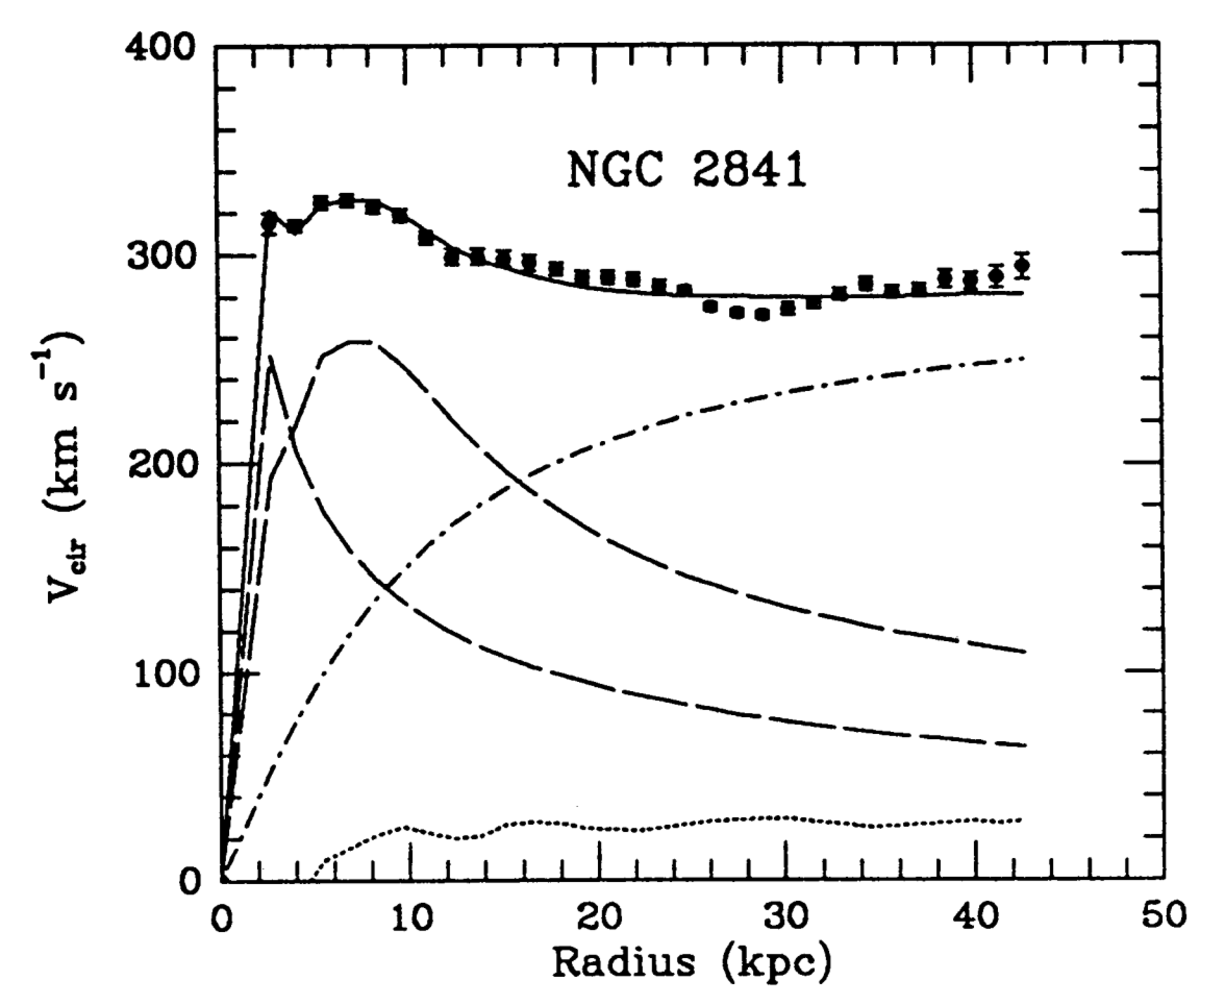
\includegraphics[width=\textwidth]{images/chapter_1/galacticCurve.pdf}
    \caption[Rotational curve of NGC 2841]{Rotational curve of NGC 2841  Predictions are shown for visible matter (dashed line), gas (dotted line), dark matter halo (dash-dot line) and total (solid line).  Data points show measurements. \cite{galacticCurve}}
    \label{fig:ch1_galacticCurve}
  \end{center}
\end{figure}

The radial velocity of a star is measured using the doppler shift and is plotted as a function of the distance from the centre of the galaxy, $r$.

\begin{eqnarray*}
  \textrm{Centripetal force} & = & \textrm{Gravitational force} \\
  \textrm{For } r<R : && \\
  \frac{\Delta m v^2(r)}{r} & = & \frac{G \Delta m M_{r<R}}{r^2} \\
  v^2(r) & = & \frac{GM_{r<R}}{r} \\
  & = & \frac{G}{r}M_s \left( \frac{r}{R} \right)^2 \\
  & = & \frac{GM_sr^2}{R^3} \\
  \textrm{So } v(r) & \propto & r \textrm{ for } r<R \\
  \textrm{For } r>R: && \\
  \frac{\Delta m v^2(r)}{r} & = & \frac{GM_s \Delta m}{r} \\
  v^2(2) & = & \frac{GM_s}{r} \\
  \textrm{So } v(r) & \propto & \frac{1}{\sqrt{r}} \textrm{ for } r>R
\end{eqnarray*}

\begin{figure}[!htb]
  \begin{center}
    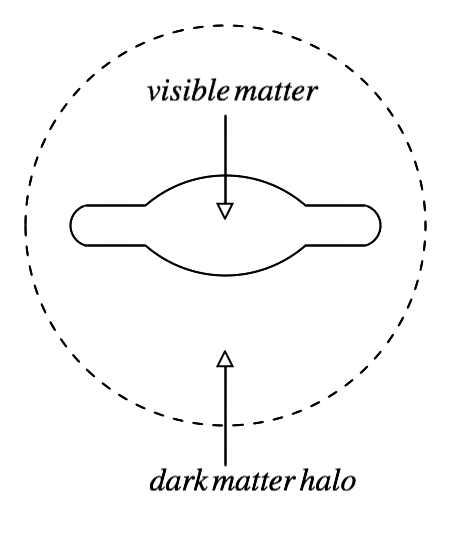
\includegraphics[width=0.8\textwidth]{images/web_feynman/image_88.png}
    \caption[Dark matter halo around a galaxy]{Dark matter halo around a galaxy.}
    \label{fig:ch1_darkMatterHalo}
  \end{center}
\end{figure}

The observed discrepency is hypothesised to be the result of dark matter.  It is thought that there is a halo of dark matter surrounding the galaxy with a matter distribution which yields the observed discrepency.

\subsection{Candidates for dark matter}

\begin{description}
  \item[Neutrinos]There is now evidence that neutrinos have mass.  However the masses are small and neutrinos are therefore relativistic particles, so this is hot dark matter which does not stay around long enough to provide gravitational binding.
  \item[Brown dwarves (Massive cool hadronic objects - MaCHOs)]Brown dwarves are like small stars which are not massive enough for nuclear burning so they appear dark.  There cannot be too many brown dwarves since there would then be too much baryonic matter which is incompatible with current understanding of the abundance of hydrogen, helium and deuterium in the early universe.  The elements were generated in the first $\simeq 900 s$.  To search for brown dwarves it is necessary to look at many stars in eg a large Magellic cloud.  If a brown dwarf passes across the line of sight of one of the stars then through gravitational lensing the light intensity from the star will increase and decrease in a characteristic way.  Brown dwarves have been observed but not in sufficient numbers to account for the amount of dark matter.
  \item[Supersymmetric particles]There are several names for such particles.  In the context of dark matter a common name is Weakly Interacting Massive Particles (WIMPs).  Alternatives include Lightest Symmetrical Particles (LSPs) and candidates thereof (neutralinos, gravitinos etc).
\end{description}

The current standard model of cosmology gives 5\% of the matter observed, 25\% dark matter and 70\% dark energy.  Where does this sub-division come from?

A survey of Type I supernovae (see figure \ref{fig:ch1_type1Supernovae}) indicates that the universe is accelerating for $z \ge 0.8 (z = \delta \lambda/\lambda)$.  The type I supernovae are like ``standard candles'' in a binary system in which matter flows from one of the stars to another and creates a thermonuclear explosion.  This constitutes the standard candle and therefore the distance can be determined.  The doppler shift gives the recessional velocity.

\begin{figure}[!htb]
  \begin{center}
    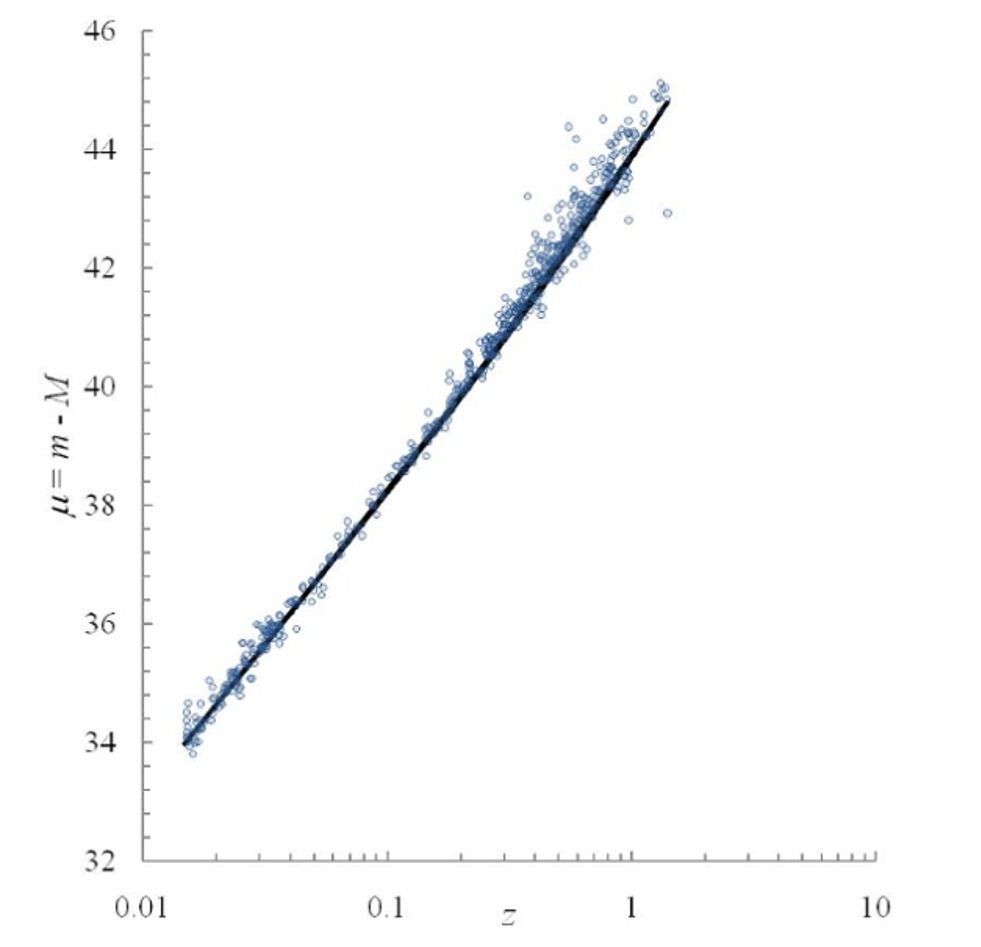
\includegraphics[width=0.5\textwidth]{images/chapter_1/type1Supernovae.pdf}
    \caption[Survey of type I supernovae]{Survey of type I supernovae. \cite{typeOneSupernovae}}
    \label{fig:ch1_type1Supernovae}
  \end{center}
\end{figure}

\subsection{Anisotropies in the cosmic microwave background and the history of the universe}

The universe is now thought to be $\sim 14 \times 10^9$ years old.  After about $350,000$ years the temperature had dropped to about $3000K$, at which point electrons and protons could combine to form hydrogen.  At this epoch, photons decoupled from matter.  Subsequently this black body spectrum cooled to $2.7K$, which is what is observed today.  This was first observed in 1965 by Perzies and Wilson, receiving the Nobel Prize in 1978.  The cosmic microwave background radiation is uniform tp $1$ part in $10^5$ in all directions.

Big bang nucleosynthesis occured in the first $900s$.  Electroweak symmetry breaking took place at $10^{-12}s$ or $E\sim 100\gev$.  The energy released by this symmetry breaking drives cosmic inflation which explains the flatness of the universe and the horizon problem.  Grand unified theory symmetry breaking occues at $10^{15} \gev$.

Anisotropies were originally measured by the COBE sattelite and by other experiments, most recently Planck (as shown in figure \ref{fig:ch1_powerSpectrum}), WMAP and Boomerang.

\begin{figure}[!htb]
  \begin{center}
    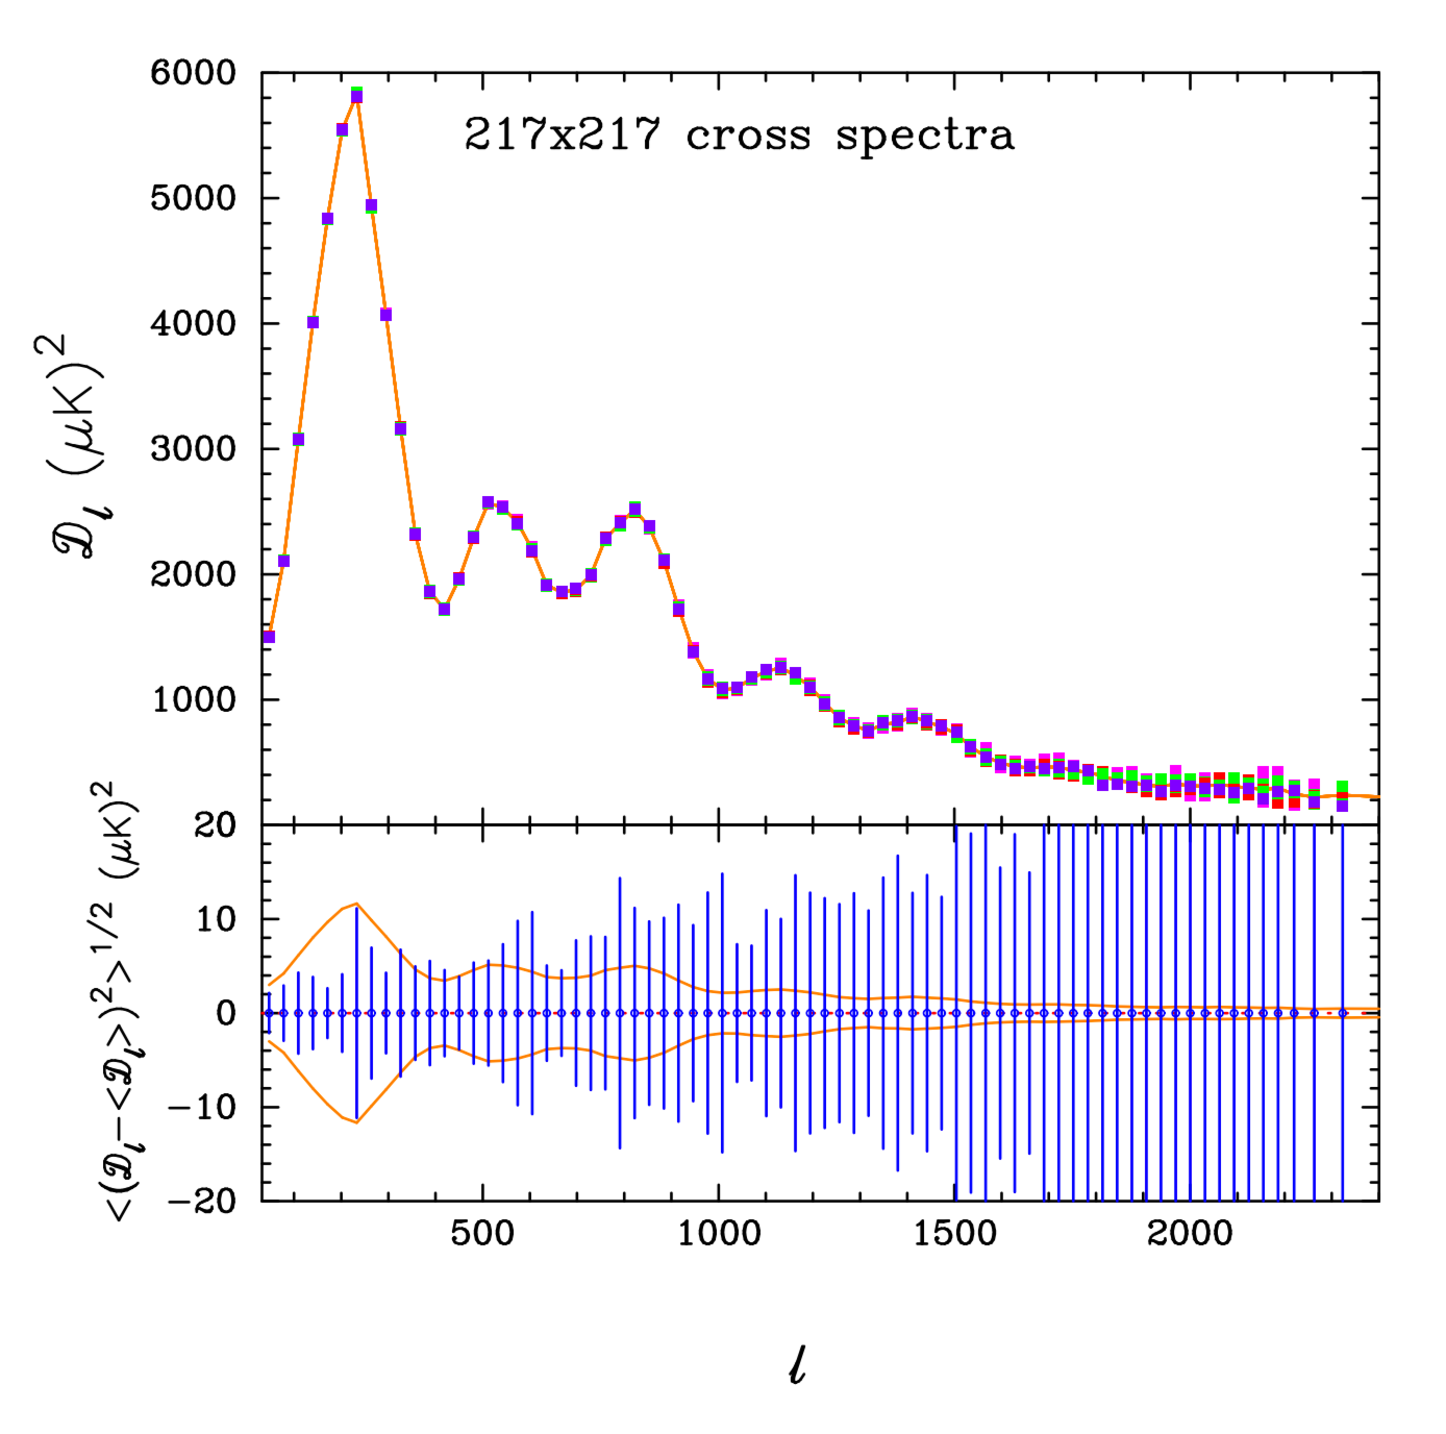
\includegraphics[width=\textwidth]{images/chapter_1/powerSpectrum.pdf}
    \caption[Cross spectra ``power spectrum'' plot (Planck)]{Cross spectra ``power spectrum'' plot (Planck). \cite{powerSpectrum}}
    \label{fig:ch1_powerSpectrum}
  \end{center}
\end{figure}

The power spectrum gives strong evidence for:
\begin{itemize}
  \item a flat universe
  \item inflation
  \item ratio of dark energy : dark matter of 70\% : 25\%
\end{itemize}

\section{The weak force}

The weak force is mediated by massive vector bosons:

\begin{eqnarray*}
  W^{\pm} & M_W & \sim 80.4 \gev \\
  Z^0     & M_Z & \sim 91.2 \gev
\end{eqnarray*}

The instrinsic strength of the force, $g_W$, is of the same order as the electromagnetic force, but the massive force carriers make it appear weak and short ranged.

For electromagnetism the strength is $\e^2/q^2$, where $q$ is the propagator momentum.  For the weak force the strength is $g^2_W/(q^2 + M^2_W)$.  Some examples of weak interactions include:

\begin{eqnarray*}
  n                   & \to & p \quad \e^- \quad \bar{\nu}_e \\
  \nu_e \quad n       & \to & p \quad \e^- \\
  \bar{\nu}_e \quad p & \to & n \quad \e^+ \\
  \bar{\nu}_e \quad u & \to & d \quad \e^+
\end{eqnarray*}

Figure \ref{fig:ch1_NToPENu} shows the Feynman diagram for a weak scattering process.

\begin{figure}[!htb]
  \begin{center}
    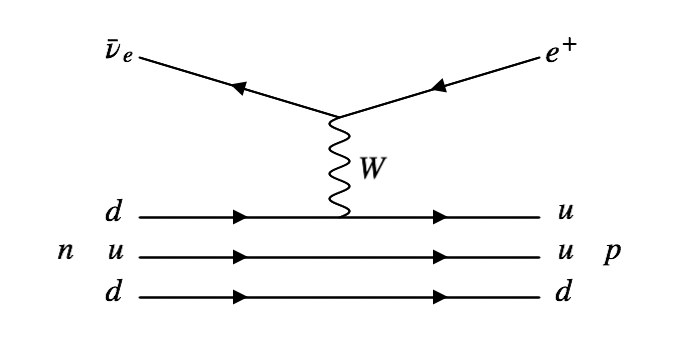
\includegraphics[width=0.8\textwidth]{images/web_feynman/image_1.png}
    \caption[Feynman diagram of proton-antineutrino scattering]{Feynman diagram showing the process $\bar{\nu}_e p \to e^+ n$.}
    \label{fig:ch1_NToPENu}
  \end{center}
\end{figure}

Some pure leptonic weak processes is shown in figures \ref{fig:ch1_NueEToNumMu} and \ref{fig:ch1_ENueToENue}.

\begin{figure}[!htb]
  \begin{center}
    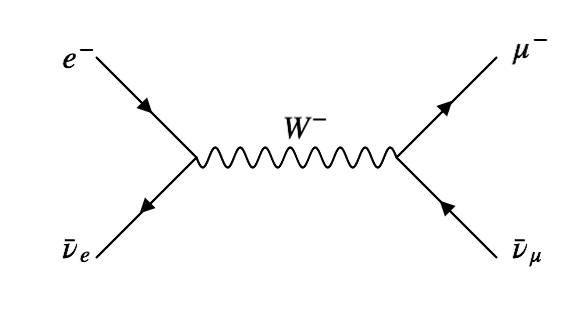
\includegraphics[width=0.8\textwidth]{images/web_feynman/image_2.png}
    \caption[Feynman diagram of lepton scattering]{Feynman diagram showing the process $\bar{\nu}_e e^- \to \bar{\nu}_\mu \mu^-$.}
    \label{fig:ch1_NueEToNumMu}
  \end{center}
\end{figure}

\begin{figure}[!htb]
  \begin{center}
    \begin{tabular}{cc}
      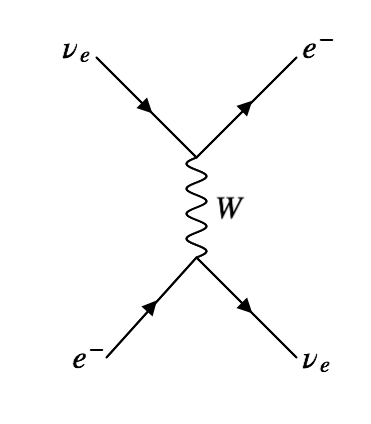
\includegraphics[width=0.4\textwidth]{images/web_feynman/image_3.png} &
      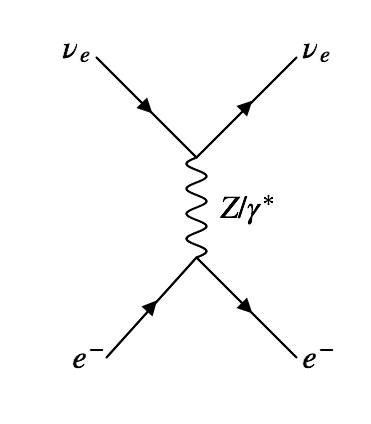
\includegraphics[width=0.4\textwidth]{images/web_feynman/image_4.png}
    \end{tabular}
    \caption[Feynman diagram of lepton scattering]{Feynman diagram showing the elastic scattering process $\nu_e e^- \to \nu_e e^-$.}
    \label{fig:ch1_ENueToENue}
  \end{center}
\end{figure}

\clearpage

\section{The electromagnetic interaction (QED)}

The electromagnetic force is mediated by the massless photon, which has an infinite range.  The coupling constant, $e$, is quantised $(0,\pm 1/3,\pm 2/3,\pm 1)$ and is not too strong, so perturbation theory works.

The strength of the force is characterised by $\alpha$:

\[
  \alpha = \frac{\e^2}{\hbar c} = \frac{\e^2_{Coulomb}}{4\pi \epsilon_0 \hbar c} = \frac{\e^2_{HL}}{4 \pi \hbar c}
\]

where $e_{Coulomb}$ is the Coulomb charge and $e_{HL}$ is the Heaviside-Lorentz charge.

In particle physics $e$ is measured in Heaviside-Lorentz units where $\hbar = c = 1$.

\[
  \textrm{Therefore } \alpha = \frac{\e^2}{4\pi} \simeq \frac{1}{137.04}
\]

\subsection{The physical meaning of \texorpdfstring{$\alpha$}{Alpha}}

$\alpha$ expresses the energy of an $\e^+ \e^- $ pair materialising for a short time in the vacuum as a fraction of the rest mass energy $m_e c^2$:

\begin{eqnarray*}
  \alpha & \sim & \frac{\e^2}{c \Delta t}\frac{1}{m_e c^2} \\
  \Delta t \Delta E & \sim & \hbar \\
  \Delta t & \sim & \frac{\hbar}{m_e c^2} \\
  \textrm{So } \alpha & \sim & \frac{\e^2}{c}\frac{m_e c^2}{\hbar}\frac{1}{m_e c^2} \\
  & = & \frac{\e^2}{\hbar c}
\end{eqnarray*}

\section{The strong force (QCD)}

Since the 1950s, it was knwon that the $\Delta^{++}(uuu)$ particle state existed at $1238 MeV$, formed in $\pi^+ p$ scattering:

\[
  \pi^+ \quad p \stackrel{\Delta^{++}}{\to} \pi^+ \quad p
\]

In the simple quark model there are 3 up quarks, each with psin$-1/2$ in the same direction.  Also in 1965 the $\Omega^-$ was discovered which consists of 3 strange quarks each with spin$-1/2$ in the same direction.  These appeared to violate the Pauli exclusion principle.

The solution was introduce 3 colour charges with the strong force mediated by massless gluons which carry colour.  The force is not of infinite rane because the strength increases with separation, leading to confinement.

\section{Local gauge invariance}

The weak, electromagnetic and strong forces all appear to arise from requiring local gauge invariance.  This means that the Lagrangians are invariant with respect to a local gauge transformation and equations of motion derived from the Lagrangian are invariant with respect to local gauge transformation.

Quantum states can be multiplied by a phase factor:

\[
  \psi'(x,t) \to \e^{iq \chi(x)}\psi(x,t)
\]

If $\chi(x,t)$ depends on space and time then the above expression is a local gauge transformation.  To allow this the electromagnetic field, $A_{\mu}$ must transform in a specific way.

In weak interactions this is not as simple.  The Lagrangian contains four massless bosons ($W^i,B$).  To allow for local gauge invariance, weak isospin and weak hypercharge matrices are required which combine with the massless vector fields to form the gauge transformation.  Symmetry breaking occurs such that $W^1_{\mu}$ and $W^2_{\mu}$ yield $W^{\pm}$ and $W^3_{\mu}$ and $B_{\mu}$ mix to yield $A_{\mu}$ and $Z^0$.  This then unifies the electromagnetic and weak interactions via the Higgs mechanism.

\section{Grand unification (GUTs)}

The GUT attemps to unify the electromagnetic, weak and strong forces.  The coupling constants evolve with energy due to loop processes, as indicated in figure \ref{fig:ch1_runningCoupling}.

\begin{figure}[!htb]
  \begin{center}
    \begin{tabular}{ccc}
      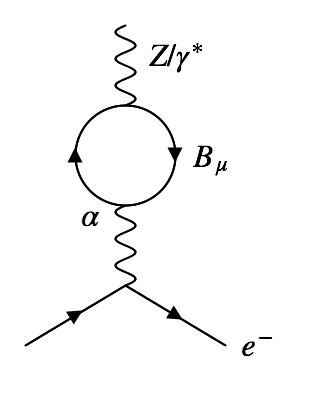
\includegraphics[width=0.3\textwidth]{images/web_feynman/image_5.png}
      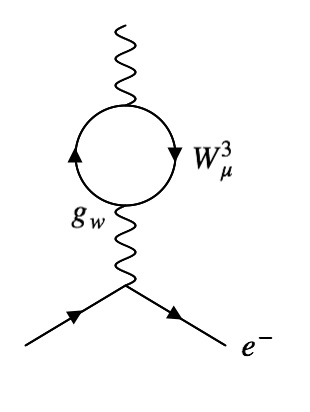
\includegraphics[width=0.3\textwidth]{images/web_feynman/image_6.png}
      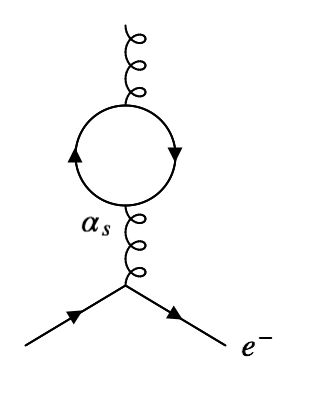
\includegraphics[width=0.3\textwidth]{images/web_feynman/image_7.png}
    \end{tabular}
    \caption[Loop processes affecting running couplings]{Typical loop processes affecting running couplings for the electromagnetic (left), weak (centre), and strong (right) processes.}
    \label{fig:ch1_runningCoupling}
  \end{center}
\end{figure}

The couplings are expected to merge at $\sim 10^{15}\gev$ according to some models, but the couplings do not come together at this energy.  The evolution of $g_1$, $g_2$, $g_3$ could coincide if supersymmetric particles exist, as shown in figure \ref{fig:ch1_SUSYUnification}.  This would then yield a grand unified group, $G$, or $SU(5)$ which is a combination of the three groups describing the three forces.  Here gauge bosons exist which would allow quarks to turn into leptons.  This would also allow protons to decay:

\[
  p \to \e^+ \quad \pi^0
\]

This decay has been extensively searched for but not observed.  This places a lower limit on the lifetime of the proton at $\tau_p > 10^{30}$ years.

\begin{figure}[!htb]
  \begin{center}
    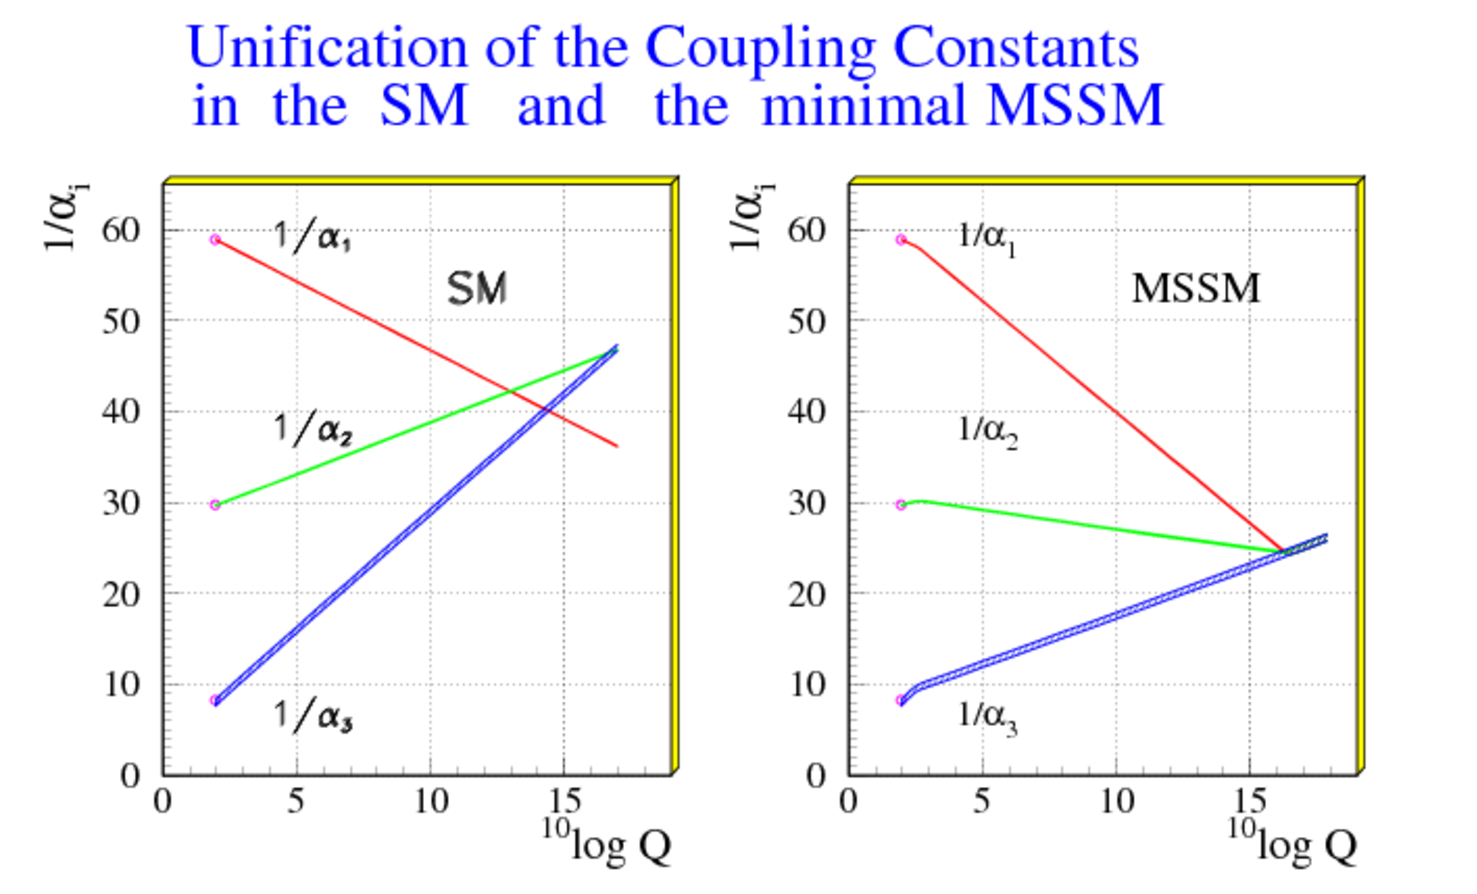
\includegraphics[width=\textwidth]{images/chapter_1/SUSYUnification.pdf}
    \caption[Running couplings and unification]{Running couplings and unification over a wide range of energies for the Standard Model (left) and with supersymmetric models (right). \cite{SUSYUnification}}
    \label{fig:ch1_SUSYUnification}
  \end{center}
\end{figure}

\cleardoublepage
% Copyright Aidan Randle-Conde 2007-2014
% http://www.aidansean.com/phd_notes
% Anyone is free to download, redistribute, edit and use these notes and the source tex files with the following restrictions:
% This 
%  This message is included in the tex source files.
%  Aidan Randle-Conde is credited as the author.
%  Images are correctly credited to their respective authors, as outlined in the references.
%  No part of these notes may be used for commercial purposes.

\chapter{Experimental concepts}

\section{Experimental possibilities}

In reality there are rather few experiemental possibilities:
\begin{itemize}
  \item Scatter one particle off another and observe the reaction
  \item Generate a particle and observe subsequent decay processes
  \item Observe neutrino oscillations
  \item Measure a particle's properties eg charge, lifetime
\end{itemize}

\section{Cross sections}

The cross section, $\sigma$, is an imaginary area surrounding a ``target'' particle through which an incident particle must pass for a particular interaction to take place.

To calculate a cross section:
\begin{itemize}
  \item Assume $N_B$ particles per incident beam bunch
  \item Assume the beam illuminates an area $A$ of the target which is of length $l$ and density $\rho$
\end{itemize}

The number of target particles that are illuminated is:

\[
  N_T = \frac{lA\rho N_A}{m}
\]

where $m$ is the molecular mass of the target nuclei and $N_A$ is Avagadro's constant.

Each of the particles is imagined to have an area $\sigma$ surrounding it.  The probability that one beam particle interacts in the area $A$ is:

\begin{eqnarray*}
  P(\textrm{Interaction}) & = & \frac{l A\rho N_A}{m}\frac{\sigma}{A} \\
  & = & \frac{l \rho \sigma N_A}{m}
\end{eqnarray*}

The total number of interactions is then:

\[
  N_I = \frac{l \rho N_A N_B \sigma}{m}
\]

To avoid shadowing $N_I$ and $l$ are replaced by $\mathrm{d}N_I$ and $\mathrm{d}l$ respectively.  In order to calculate the number of interactions per second in a general collider it is necessary to make the expression symmetrical with respect to the beam and target:
\begin{itemize}
  \item Assume the particle densities in the beam and target are $\rho_B$ and $\rho_T$ respectively
  \item Assume the interactions are occuring in a volume $V$ with a cross-sectional area A
  \item Assume the beam travels with a relative speed $u$
\end{itemize}

The number of target particles in the volume $V$ is $\rho_T V$, so the probability of one beam particle interacting in the area $A$ is $\rho_T V \sigma / A$.  In $1\units{s}$ there are $uA\rho_B$ particles.

\[
  \Rightarrow \frac{\mathrm{d}n}{\mathrm{d}t} = u\sigma V \rho_B \rho_T
\]

In a collider there are $n$ bunches containing $N_B$ particles rotating at $u \sim c$.  A second beam rotates in the opposite direction.  The probability of an interaction is $\sigma N_B / A$ in one bunch of the second beam where $A$ is the cross-section interaction region.  In $1s$ $f$ bunches (where $f$ is the rotation frequency) pass through the bunch in the second beam:

\begin{eqnarray*}
  \Rightarrow \frac{\mathrm{d}N_I}{\mathrm{d}t} & = & \frac{f N_B N_B n \sigma}{A} \\
  & = & L \sigma
\end{eqnarray*}
where the luminosity, $L$, is given by:

\begin{eqnarray}
  L & = & \frac{n N^2_B f}{A} \nonumber \\
  L & = & \frac{1}{\sigma}\frac{\mathrm{d}N_I}{\mathrm{d}t} \label{eq:luminosity}
\end{eqnarray}

(\ref{eq:luminosity}) is the formal definition of the luminosty.  The unit of cross-section is the barn, where $1 bn = 10^{-28}\units{m}^2$ and the units of $L$ are $\units{bn}^{-1}\units{s}^{-1}$.  The luminosity can be quoted in inverse picobarns per second and the integrated luminosity can be quoted in inverse picobarns.

\subsection{Scattering pions and nucleons}

Pions and nucleaons interact strongly, with cross sections shown in figure \ref{fig:ch2_pionNucleonScattering}.  According to the old understanding of the strong interaction two protons may exchange a $\pi^0$ to form a $\Delta^{++}$ which subsequently decays to a proton and $\pi^0$, as shown in figure \ref{fig:ch2_PPToPPPi0}.

\begin{figure}[!htb]
  \begin{center}
    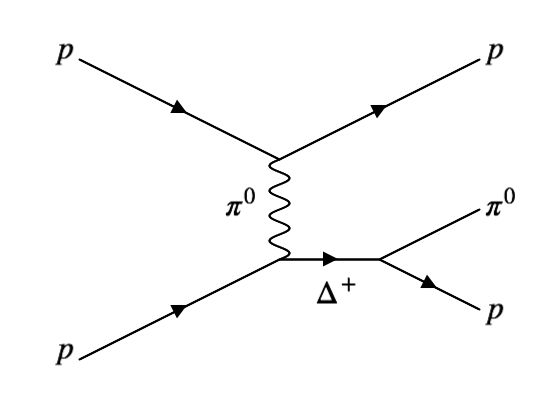
\includegraphics[width=0.8\textwidth]{images/web_feynman/image_8.png}
    \caption[Feynman diagram of proton-proton scattering]{Feynman diagram of proton-proton scattering, with the formation of the $\Delta^+$ resonance and emission of a $\pi^0$ meson.}
    \label{fig:ch2_PPToPPPi0}
  \end{center}
\end{figure}




\begin{figure}[!htb]
  \begin{center}
    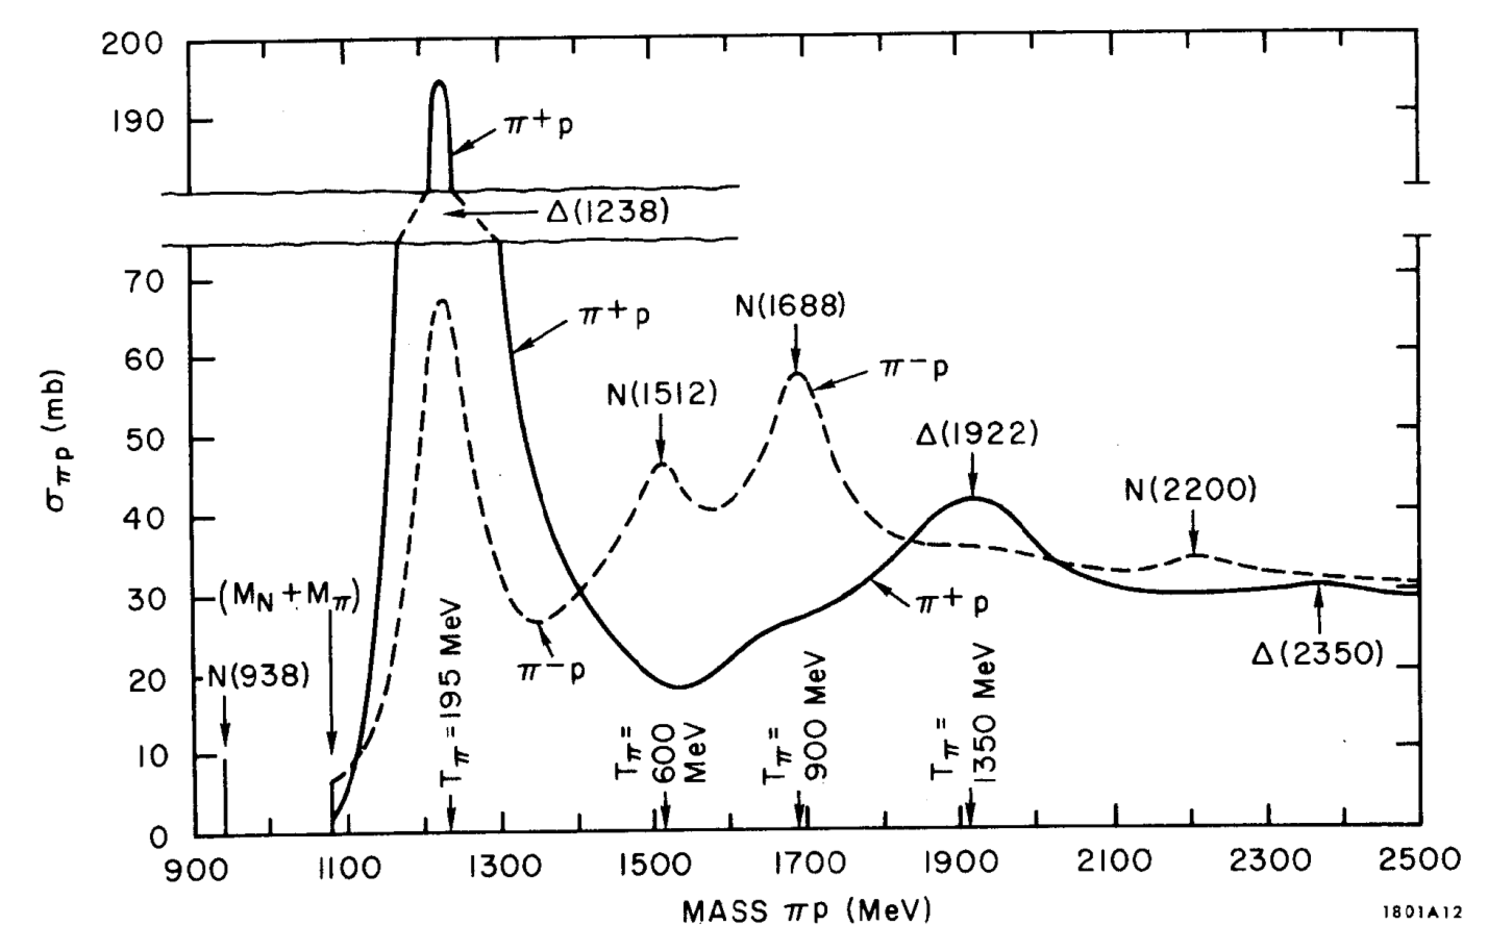
\includegraphics[width=\textwidth]{images/chapter_2/pionNucleonScattering.pdf}
    \caption[Pion-nucleon scattering cross section]{Pion-nucleon scattering cross section for positively and negatively charged pions incident on fixed targets. \cite{pionNucleonScattering}}
    \label{fig:ch2_pionNucleonScattering}
  \end{center}
\end{figure}

The cross sections for various interactions are:

\[
  \sigma_{pp} > \sigma_{np} \gg \sigma_{\gamma p} \gg \sigma_{\gamma \gamma}
\]

Detectors are based on such particle collisions and interactions and the radiation length is different for different materials eg high-energy electrons ($> \gev$) lose the same fraction of energy in $18 cm$ of water as in $2.8mm$ of lead.  In matter particles lose energy by ionisation, which is expressed as $\mathrm{d}E / \mathrm{d} x$, which is largely a function of the velocity of the particle, as shown in figure \ref{fig:ch2_energyLoss}.

\begin{figure}[!htb]
  \begin{center}
    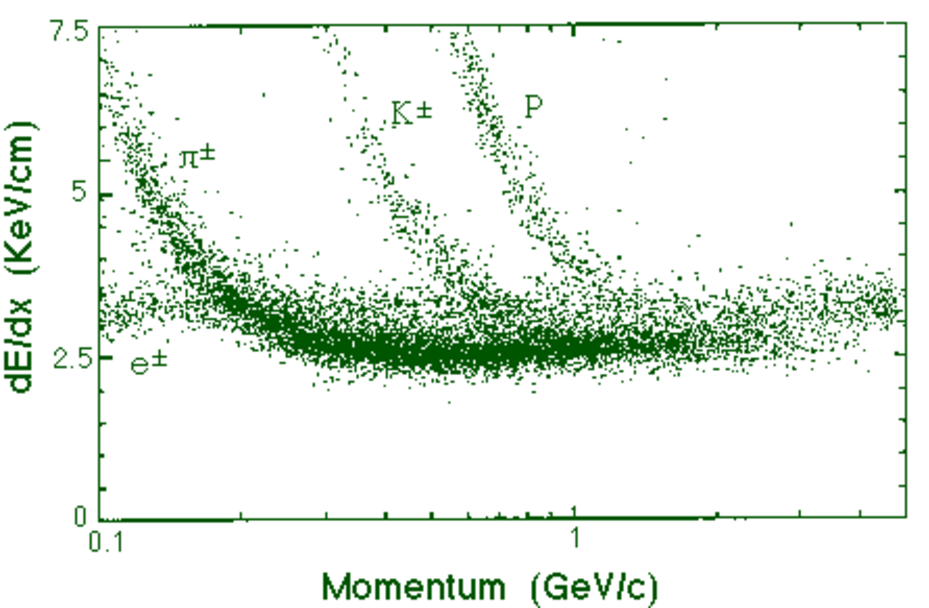
\includegraphics[width=0.5\textwidth]{images/chapter_2/Argus.pdf}
    \caption[Energy loss as a function of momentum]{Energy loss as a function of momentum, measured in the Argus drift chamber. \cite{energyLoss}}
    \label{fig:ch2_energyLoss}
  \end{center}
\end{figure}

\section{Natural units and conversion factors}

In quantum mechanics the expressions for energy and momentum can be expressed as:

\[
  \begin{array}{cccccl}
  E_{\nu} & = & hf & = & \hbar \omega    & \textrm{Planck's law} \\
  p_{\nu} & = & h/\lambda & = & \hbar k & \textrm{De Broglie's relation}
  \end{array}
\]

Travelling quantum waves are of the form:

\begin{eqnarray*}
  \psi & = & A \e^{i\left( kx - \omega t\right)} \\
  & = & A \e^{i/\hbar\left(px - Et\right)}
\end{eqnarray*}

And for light $c = f\lambda = \omega / k$.

It is conventient to set $\hbar = c = 1$.  Consider the units of $c\hbar$:

\begin{eqnarray*}
  [c\hbar] & = & [L] [T^{-1}] [E] [T] \\
  & = & [L] [E] \\
  c & = & 3 \times 10^8 \units{ms}^{-1} \\
  \hbar & = & 6 \times 10^{-25} \units{\gev s} \\
  c \hbar & = & 1.97 \times 10^{-16} \units{\gev m}
\end{eqnarray*}

Thus setting $c = \hbar = 1$ gives $1 = 1.97 \times 10^{-16} \gev\units{m}$.

Other useful conversion factors include:

\[
  \begin{array}{cccl}
  \frac{1}{\left( \gev \right)^2} & = & 3.89 \times 10^{-32}\units{m}^2 & = 0.389 \units{mb} \\
  \frac{1}{\gev} & = & 6.6 \times 10^{-5} \units{s} & 
  \end{array}
\]

\cleardoublepage
\chapter{Experiments of the past fifty years}

Until the 1950s particle physics was studied by observing cosmic rays in cloud chambers and nuclear emulsion.  After 1945 nucleon-nucleon scattering experiements were carried out at cyclotrons and energies became high enough for pions to be produced.  Then pion-nucleon scattering was studied.

\[
  \textrm{In 1952 } \pi^+ \quad p \stackrel{\Delta^{++}}{\to} \pi^+ \quad p
\]

Also, from electron beams photons could be produced:

\[
  \gamma \quad p \stackrel{\Delta^+}{\to} \gamma \quad \gamma \quad p \quad (\textrm{via } \Delta^+ \to p \quad \pi^0 )
\]

although the rate of production via $\gamma$ processes is much lower because of the strength of the electromagnetic coupling.

Other processes were also observed:
\begin{eqnarray*}
  \pi^+ & \to & \mu^+ \quad \nu_{\mu} \\
  \mu^+ & \to & \e^+ \quad \bar{\nu}_{\mu} \quad \nu_e
\end{eqnarray*}

where the latter process is a purely leptonic process and so provoked much theoretical interest.

In 1956 parity violation in the weak interaction was discovered (Lee and Young received the Nobel Prize.)  The experiement was studying the $\beta$ decay of polarised Cobalt $60$ nuclei.  An anistropy was discovered in the electron spectroscopy with respect to the $^{60}\textrm{Co}$ nuclear spin. The spins of the particles are shown in figure \ref{fig:ch3_CoNi}.

\begin{figure}
  \begin{center}
    \begin{tabular}{ccccccc}
      $\textrm{Co}$      &               & $\textrm{Ni}$      &     &            &               &                   \\
                         &               &                    &     & $\Uparrow$ & $\bar{\nu}_e$ & $\uparrow$        \\
      $\Big{\Uparrow}$   & $\rightarrow$ & $\Big{\Uparrow}$   & $+$ &            &               &                   \\
                         &               &                    &     & $\Uparrow$ & $e^-$         & $\downarrow$      \\
      $J=5$              &               & $J=4$              &     &            &               &                   \\
      &&&&&&\\
      $^{60}\textrm{Co}$ & $\rightarrow$ & $^{60}\textrm{Ni}$ & $+$ & $(e^-)_L$  & $+$           & $(\bar{\nu}_e)_R$ \\
    \end{tabular}
  \caption{Parity violating decay $^{60}\textrm{Co}\to ^{60}\textrm{Ni}\, e^- \,\bar{\nu}_e$}
  \label{fig:ch3_CoNi}
  \end{center}
\end{figure}

\[
  ^{60}\textrm{Co} \to ^{60}\textrm{Ni}* \Big(\e^-\Big)_L \Big(\bar{\nu}_e\Big)_R
\]

By the 1960s kaon beams were generated at synchotrons and this confirmed the discovery of strangeness that was observed in cosmic ray experiments.  It also established (in the experimentalists' eyes) the quark substructure of hadrons ie hadrons were made of $q\bar{q}$ pairs (mesons) and $qqq$ triplets (baryons) where $q$ is a $u$, $d$ or $s$ quark.  Theorists regarded the evidence for strangeness as establishing the $SU(3)$ flavour symmetry, which is now known to have been accidental.  This symmetry arises because the constituent masses of $u$ and $d$ quarks are about the same and the mass of the $s$ quark is somewhat heavier.

\section{Mesons and baryons}

Consider $q\bar{q}$ systems consisting of $u$ and $d$ quarks.  The strong isospin doublet is:

\[
  2 = 
  \left(
    \begin{array}{c}
    u \\
    d
    \end{array}
  \right)
    \begin{array}{ccc}
    I_3 & = & \pm \frac{1}{2} \\
    I & = & \frac{1}{2}
    \end{array}
\]

Assume that the strong isospin is conserved (which is accidental, but works as the $u$ and $d$ quarks have nearly the same mass.)  This doublet is combined with the antiquark doublet which is:

\[
  \bar{2} = 
  \left(
    \begin{array}{c}
    -\bar{d} \\
    \bar{u}
    \end{array}
  \right)
    \begin{array}{c}
    ^{ \frac{1}{2}} \\
    _{-\frac{1}{2}}
    \end{array}
\]

In this form the raising and lowering operators act on the $2$ doublet in the same way for the $\bar{2}$ antiquark doublet.  The minus sign on $\bar{d}$ arises because of a rotation in isospin space:

\begin{eqnarray*}
  \left(
    \begin{array}{c}
    u \\
    d
    \end{array}
  \right)'
  & = &
  \e^{-i \pi \tau_z/2}
  \left(
    \begin{array}{c}
    u \\
    d
    \end{array}
  \right)
  \\
  & = &
  I\left( \cos \frac{\pi}{2} -i\frac{\tau}{2} \sin \frac{\pi}{2} \right)
  \left(
    \begin{array}{c}
    u \\
    d
    \end{array}
  \right)
  \\
  \Rightarrow
  \left(
    \begin{array}{c}
    u \\
    d
    \end{array}
  \right)'
  & = &
  \left(
    \begin{array}{cc}
    0 & -1 \\
    1 & 0
    \end{array}
  \right)
  \left(
    \begin{array}{c}
    u \\
    d
    \end{array}
  \right)
  \\
  & = &
  \left(
    \begin{array}{c}
    -d \\
    u
    \end{array}
  \right)
  \\
  u' & \to & -d \\
  d' & \to & u
\end{eqnarray*}

Suppose $\bar{2}$ had been defined as:

\[
  \bar{2} = 
  \left(
    \begin{array}{c}
    \bar{d} \\
    \bar{u}
    \end{array}
   \right)
\]

Then the transformation would be:

\begin{eqnarray*}
  \bar{d}' & \to & -\bar{u} \\
  \bar{u}' & \to & \bar{d}
\end{eqnarray*}

The $\bar{2}$ system therefore transforms in the same way as a the $2$ system:

\begin{eqnarray*}
  \left(
    \begin{array}{c}
    -\bar{d} \\
    \bar{u}
    \end{array}
  \right)
  & = &
  \left(
    \begin{array}{cc}
    0 & -1 \\
    1 & 0
    \end{array}
  \right)
  \left(
    \begin{array}{c}
    -\bar{d} \\
    \bar{u}
    \end{array}
  \right)
  \\
  & = &
  \left(
    \begin{array}{c}
    -\bar{u} \\
    -\bar{d}
    \end{array}
  \right) \\
  -\bar{d}' & \to & -\bar{u} \\
  \bar{u}'  & \to & -\bar{d}
\end{eqnarray*}

Now $2$ and $\bar{2}$ can be combined to form a representation of the $\pi$ mesons:

\[
  \begin{array}{ccccc}
           & ( & u         & d         & ) \\
  \left( \begin{array}{c}-\bar{d} \\ \bar{u} \end{array} \right) & \Bigg( 
  & \begin{array}{c} -u\bar{d} \\ u\bar{u} \end{array}
  & \begin{array}{c} -d\bar{d} \\ d\bar{u} \end{array} & \Bigg) \\
  \end{array}
\]

\begin{eqnarray*}
  \pi^+ & = & -u\bar{d} \\
  \pi^- & = & d\bar{u} \\
  \pi^0 & = & \frac{1}{\sqrt{2}}\left( u\bar{u} - d\bar{d} \right)
\end{eqnarray*}

There is an isospin doublet to represent the antiquarks in $SU(2)$ and not in any other $SU(n)$.  In $SU(3)$ flavour symmetry:

\begin{eqnarray*}
  3 & = &
  \left(
    \begin{array}{c}
    u \\
    d \\
    s
    \end{array}
  \right)
  \\
  \bar{3} & = &
  \left(
    \begin{array}{c}
    \bar{u} \\
    \bar{d} \\
    \bar{s}
    \end{array}
  \right)
\end{eqnarray*}

To construct the $q\bar{q}$ states in $SU(3)$:

\[
  \begin{array}{cccccc}
    & ( & u & d & s & ) \\
    \left(
    \begin{array}{c}
      \bar{u} \\
      \bar{d} \\
      \bar{s}
    \end{array}
    \right)
    &
    \Bigg(
    &
    \begin{array}{c}
      u\bar{u} \\
      u\bar{d} \\
      u\bar{s}
    \end{array}
    &
    \begin{array}{c}
      d\bar{u} \\
      d\bar{d} \\
      d\bar{s}
    \end{array}
    &
    \begin{array}{c}
      s\bar{u} \\
      s\bar{d} \\
      s\bar{s}
    \end{array}
    &
    \Bigg)
  \end{array}
\]

The non diagonal elements are easily identified as the following particles:

\begin{eqnarray*}
  s\bar{u} = K^- & & u\bar{s} = K^+ \\
  d\bar{s} = \bar{K}^0 & & s\bar{d} = K^0 \\
  u\bar{d} = \pi^+ & & d\bar{u} = \pi^-
\end{eqnarray*}

There is also a symmetric state:

\[
  \eta_1: \quad \frac{1}{\sqrt{3}}\left( u\bar{u} + d\bar{d} + s\bar{s} \right)
\]

This is called the $SU(3)$ singlet state.  The final neutral state is:

\[
  \eta_8: \quad \frac{1}{\sqrt{6}}\left(u\bar{u} + d\bar{d} + 2s\bar{s} \right)
\]

This is constructed to be orthogonal to the $\pi^0$ and the singlet state.  The mesons are shown in figures \ref{fig:ch3_mesonNonetSpin0} and \ref{fig:ch3_mesonNonetSpin1}.

\begin{figure}[!htb]
  \begin{center}
    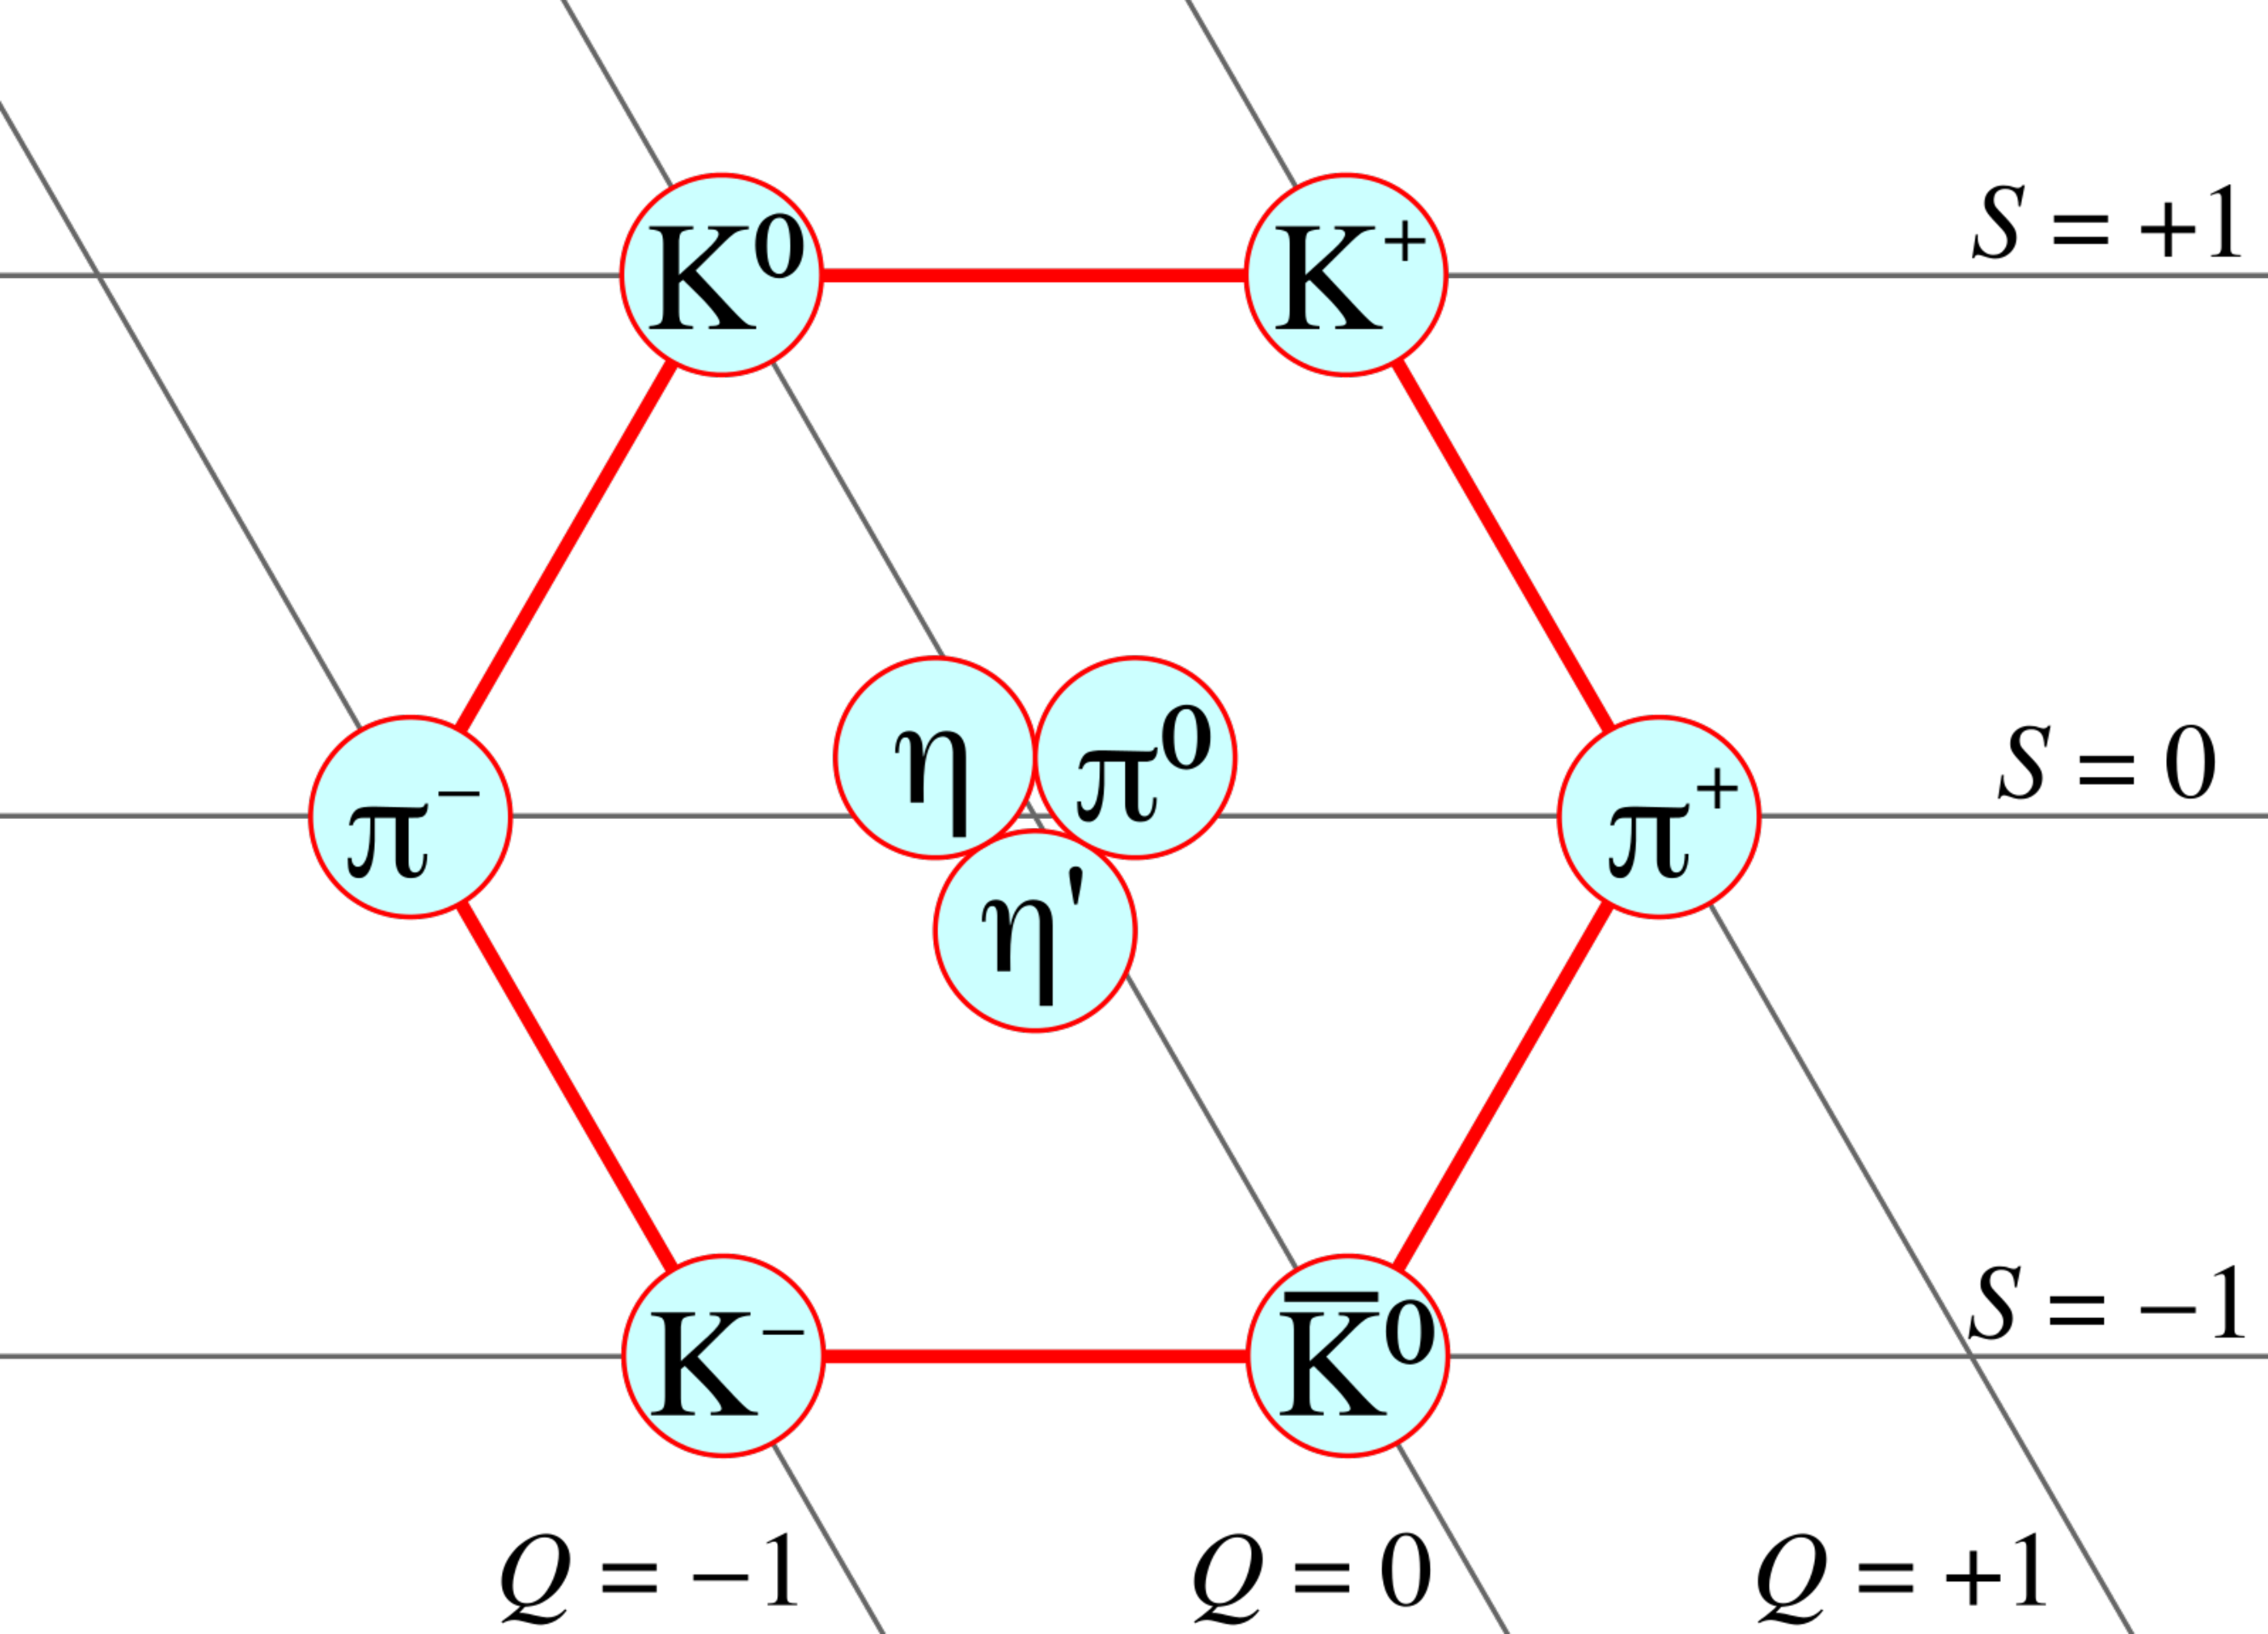
\includegraphics[width=0.5\textwidth]{images/chapter_3/MesonNonetSpin0.pdf}
    \caption[$J^{P}=0^-$ meson nonet]{The pseudoscalar $J^{P}=0^-$ meson nonet. \cite{mesonNonets}}
    \label{fig:ch3_mesonNonetSpin0}
  \end{center}
\end{figure}

\begin{figure}[!htb]
  \begin{center}
    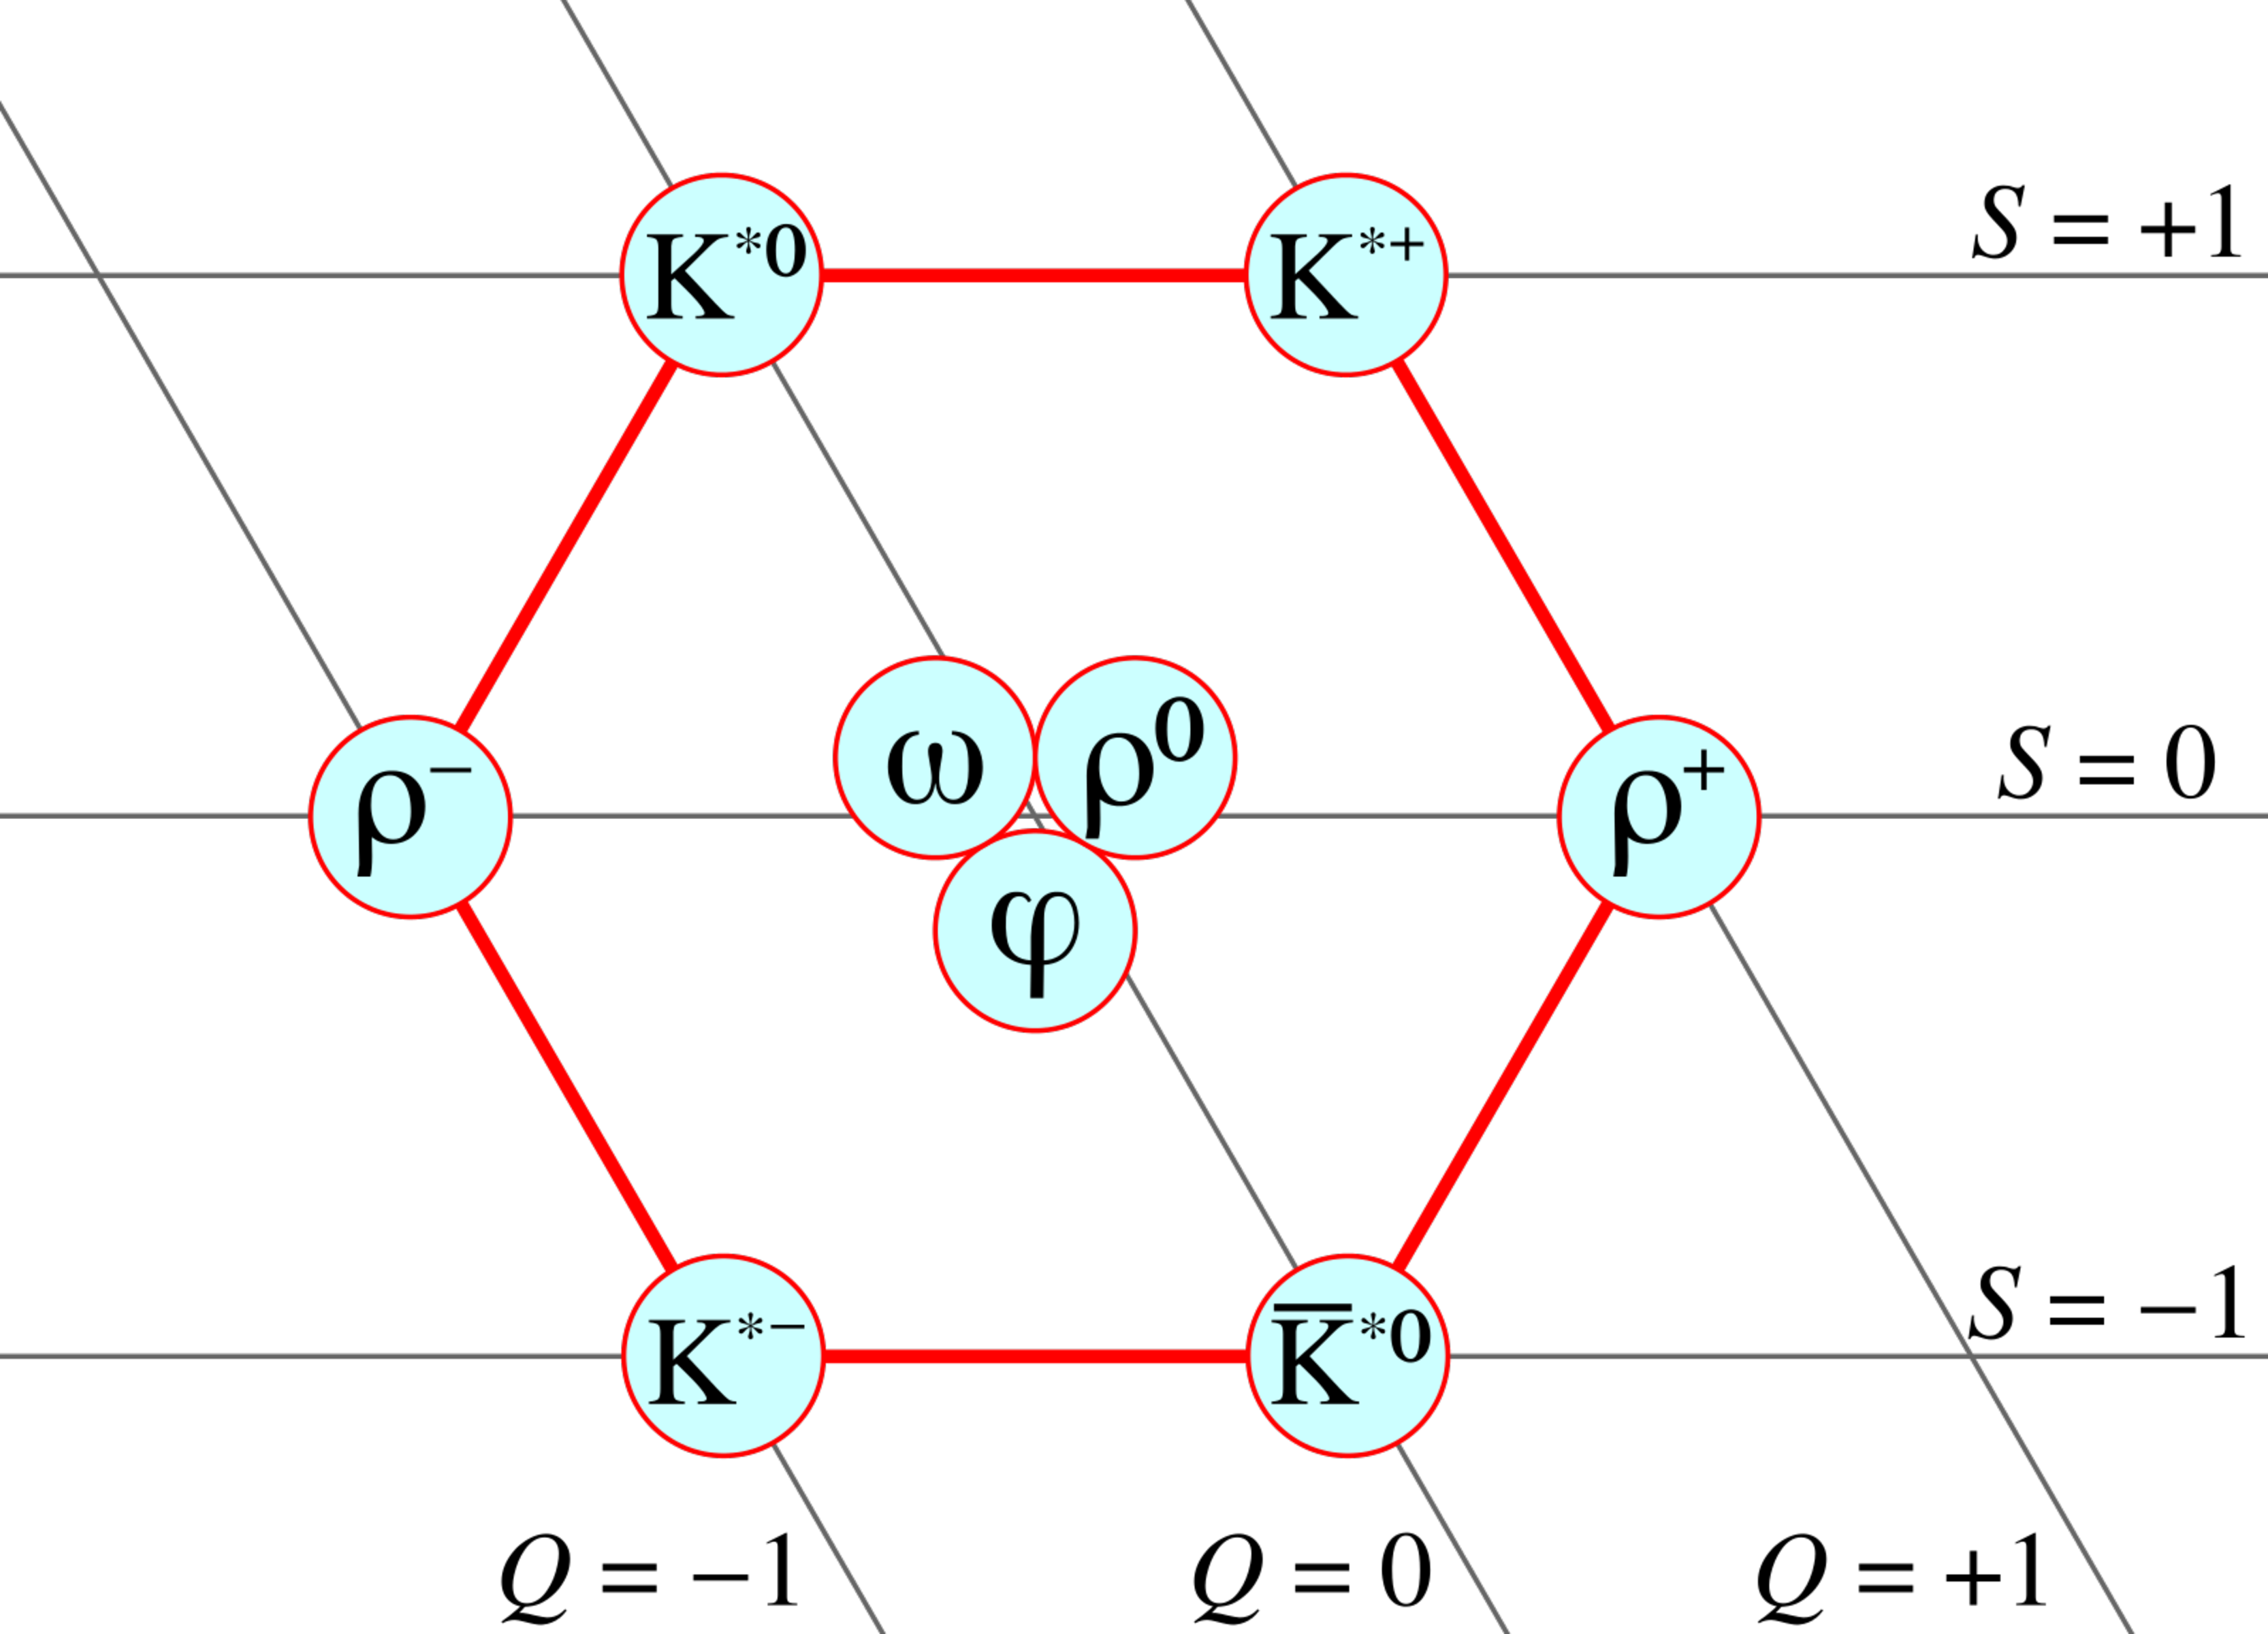
\includegraphics[width=0.5\textwidth]{images/chapter_3/MesonNonetSpin1.pdf}
    \caption[$J^{P}=1^-$ meson nonet]{The vector $J^{P}=1^-$ meson nonet. \cite{mesonNonets}}
    \label{fig:ch3_mesonNonetSpin1}
  \end{center}
\end{figure}

\clearpage

\section{Neutrino experiments}

\subsection{The Gargamelle experiment}

Using the CERN proton synchrotron, protons were extracted from the accelerator and impinged on a thin Beryllium target within a neutrino horn.  In the targets $\pi$s and $K$s were created and the horn partially selected either positive or negative charges.  The partially focussed $\pi^+$ beam decayed to $\mu^+ \nu_{\mu}$.  An iron shield filtered out the remaining hadrons and muons.  Measurements of the muon tracks enabled the neutrino spectrum to be determined.  The neutrios then passed into the large heavy liquid bubble chamber, Gargamelle.  Scattering via the exchange of the $W^{\pm}$ was expected, but scattering via the $Z^0$ was also observed, as shown in figure \ref{fig:ch3_NumPToMuHad}.

\begin{figure}[!htb]
  \begin{center}
    \begin{tabular}{cc}
      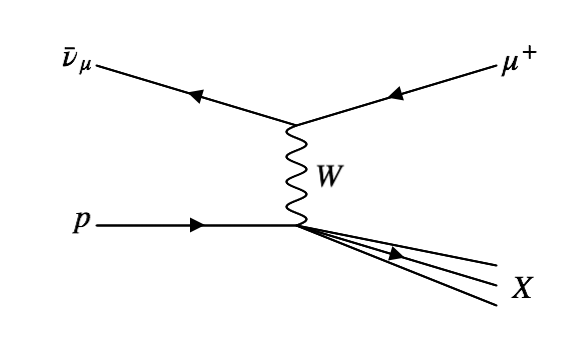
\includegraphics[width=0.45\textwidth]{images/web_feynman/image_9.png} &
      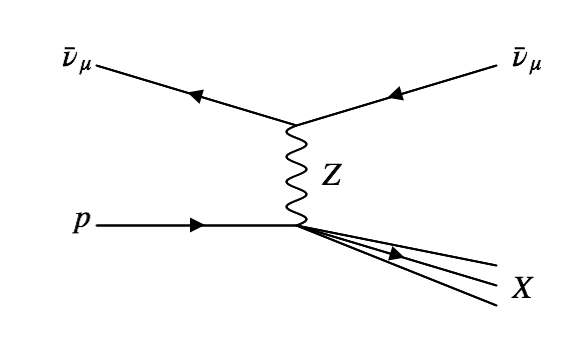
\includegraphics[width=0.45\textwidth]{images/web_feynman/image_10.png}
    \end{tabular}
    \caption[Neutrino-nucleon scattering at Gargamelle]{Neutrino-nucleon scattering at Gargamelle, with a charged current interaction (left), and neutral current interaction (right).}
    \label{fig:ch3_NumPToMuHad}
  \end{center}
\end{figure}

\subsection{Underground experiments}

Solar neutrinos are produced primarily by the following reaction:

\[
  p \quad p \to d \quad \e^+ \quad \nu_e
\]

Atmospheric neutrinos are produced primarily by proton bombardment of the upper atmosphere:

\[
  \begin{array}{ccccc}
  p \quad N & \to & \pi^+/K^+ \quad \textrm{H}      &                 & \\
      &     &  \hookrightarrow & \mu^+ \quad \nu_{\mu} & \\
      &     &                  & \hookrightarrow & \e^+ \quad \bar{\nu}_{\mu} \quad \nu_e
  \end{array}
\]

Naïvely, it is expected that the production rate would be:

\[
  \frac{\nu_e}{\nu_{\mu}} \sim \frac{1}{2}
\]

The ratio has been measured by Superkamikande to be closer to $1$, demonstrating that $\nu_{\mu}$ neutrinos were missing and also measured an azimuthal variation.  ie the experiment measured the number of neutrinos $N(\nu_{\mu})$ and $N(\nu_e)$ from the atmosphere (above) and the other side of the Earth (below.)  About half from the other side of the Earth were lost, suggesting that that neutrinos oscillated into $\nu_{\tau}$.  The oscillations imply that neurinos have mass and as such must have a velocity $\beta < 1$.

A large detector of water was used to look for the processes:

\begin{eqnarray*}
  \nu_{\mu} \quad N & \to & \mu^- \quad \textrm{H} \\
  \nu_e     \quad N & \to & \e^-  \quad \textrm{H}
\end{eqnarray*}

Both muons and electrons were detected by $\sim 5,000$ phototubes by considering their characteristic signals for Cerenkov light.  The muon signal rings are sharp whereas those for electrons are diffuse.

\subsection{Solar neutrinos}

In the experiment by Ray Davis mainly ``high'' energy ($14 \mev$) neutrinos were used from a process:

\[
  \begin{array}{cccc}
  p \quad ^7\textrm{Be} & \to & ^8\textrm{Be} \quad \gamma & \\
               &     & \hookrightarrow   & ^8\textrm{Be} \quad \e^+ \quad \nu_e
  \end{array}
\]

The group looked for the reaction:

\[
  \nu_e \, {}^{37}\textrm{Cl} \to \e^- \quad \phantom{}^{37}\textrm{Ar}
\]

The neutrinos were impinging on a tank of $C_2Cl_4$.  There were not as many such reactions as expected according to the Standard Model.

To detect low energy neutrinos, tanks of Galium were used:

\[
  \nu_e \quad \textrm{Ga} \to \textrm{Ge} \quad \e^-
\]

These processes were also observed at a lower than expected rate.

In the Sudbury Neutrino Observatory (SNO) a tank of heavy water ($\textrm{D}_2\textrm{O}$) was used.  The following reaction was detected:

\[
  \nu_e \quad n \to \e^- \quad p
\]

Again, a deficit of electron neutrinos was observed.  Around $1/3$ of the expected signal was observed.  Combined with the results from Superkamiokande this explains the solar neutrino problem where $\sim 1/3 \nu_e$ are observed and $\sim 2/3 \nu_e$ oscillate into $\nu_{\mu}$ and $\nu_{\tau}$.

The results at SNO were further confirmed when salt ($\textrm{NaCl}$) was added to the water, increasing the sensitivity to $\nu_{\mu}$ and $\nu_{\tau}$:

\begin{eqnarray*}
  \nu_{e/\mu/\tau} \quad n       & \to & \nu_{e/\mu/\tau} \quad n_{scattered} \\
  \textrm{Then } ^{37}\textrm{Cl} \quad n & \to & ^{38}\textrm{Be} \quad \gamma
\end{eqnarray*}

This was then consistent with the expected solar flux.

Further neutrino oscillation experiments are ongoing at reactors (a good source of copious low energy neutrinos from $b$ decay) and at accelerators such as MINOS.

\section{Colliding beam experiments (Some fixed target)}

There are various different types of colliding beams which have different properties and can probe different phenomena.  They can be classified into three types:

\begin{description}
  \item[$\e^+ \e^-$] Purely leptonic beams give rise to "clean" output and also have a controled centre of mass energy.  There is a large discovery potential, however there are limits due to synchrotron  radiation, so future developments will lead to linear colliders.
  \item[$NN(pp)$]   Purely hardonic beams are not as clean and do not have a well defined centre of mass energy.  However there is a large discovery potential due to the possibility of much higher energies.
  \item[$lN$]      A mixed pair of beams allows probing of the partons.
\end{description}

\subsection{Lepton-nucleon colliders}

In the late 1960s and the early 1970s deep inelastic scattering experiments using lepton beams of electrons, neutrinos and also muons were used to probe the structure of the proton and neutron.  It looked as if scattering occured on pointlike objects in the nucleon and around 50\% of the nucleon interacted in this way.  The remaining 50\% was made up of gluons.  This was the beginnings of quantum chromodynamics (QCD).

At HERA, this has been advanced further in $ep$ collisions.  Electrons (or positrons) of energies at $27.5 \gev$ collide with protons at $920 \gev$, yielding a centre of mass energy of around $320 \gev$.  There are two multipurpose colliding beam experiments which measure a wide range of phenomena such as proton and photon structure; many other aspects of QCD; electroweak physics and searches for effects beyond the Standard Model (eg leptoquarks).

The structure of the proton has been measured over a vast kinematic range compared to the first measurements in the 1960s, as shown in figure \ref{fig:ch3_F2}.  A typical deep inelastic scattering process is shown in figure \ref{fig:ch3_EPToEHad}.

\begin{figure}[!htb]
  \begin{center}
    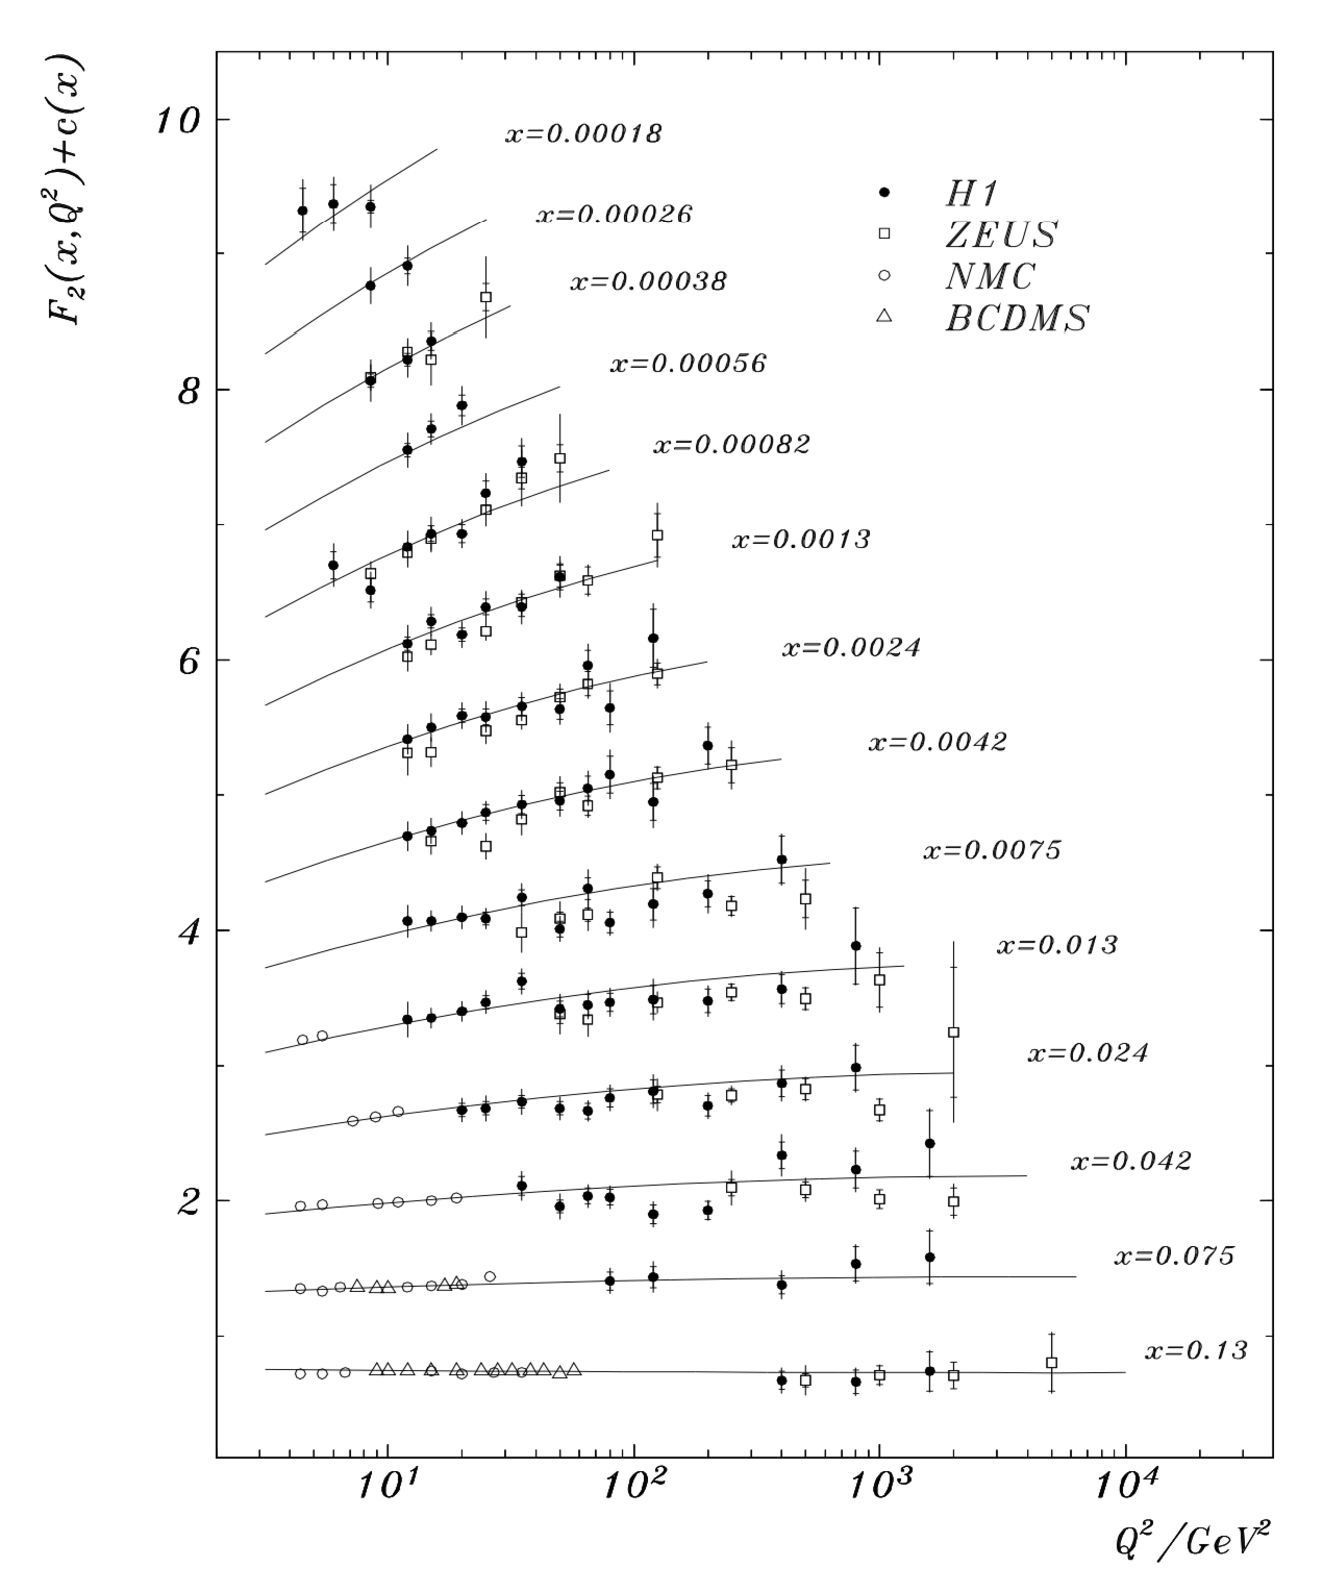
\includegraphics[width=0.7\textwidth]{images/chapter_3/F2.pdf}
    \caption[The structure of the proton]{The structure of the proton, $F_2$, as a function of $Q^2$. \cite{F2}}
    \label{fig:ch3_F2}
  \end{center}
\end{figure}

\begin{figure}[!htb]
  \begin{center}
    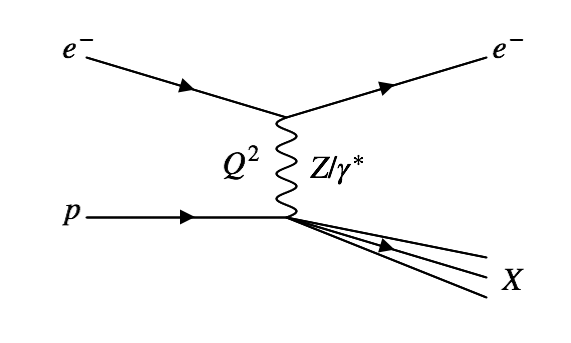
\includegraphics[width=0.8\textwidth]{images/web_feynman/image_11.png}
    \caption[Deep inelastic scattering process]{Deep inelastic scattering process for $e^-p\to e^-X$, where $X$ is any hadronic system allowed by conservation laws.}
    \label{fig:ch3_EPToEHad}
  \end{center}
\end{figure}

$x$ is the proton's momentum fraction carried by the struck quark.
$Q^2$ is the four momentum transfer, essentially related to the wavelength of the probing photon.  A high value for $Q^2$ implies a high resolving power.

This gives us precise knowledge of the structure of matter which is one of the fundamental goals of physics.  Also practically many colliders use protons (eg LHC) so it is useful for understand the structure of what is being collided.

Demonstration of the unification of the electroweak force is shown in figure \ref{fig:ch3_electroweakUnification}.  The processes became the ``same'' at $M^2_{W,Z} \sim 10^4 \gev^2$.

\begin{figure}[!htb]
  \begin{center}
    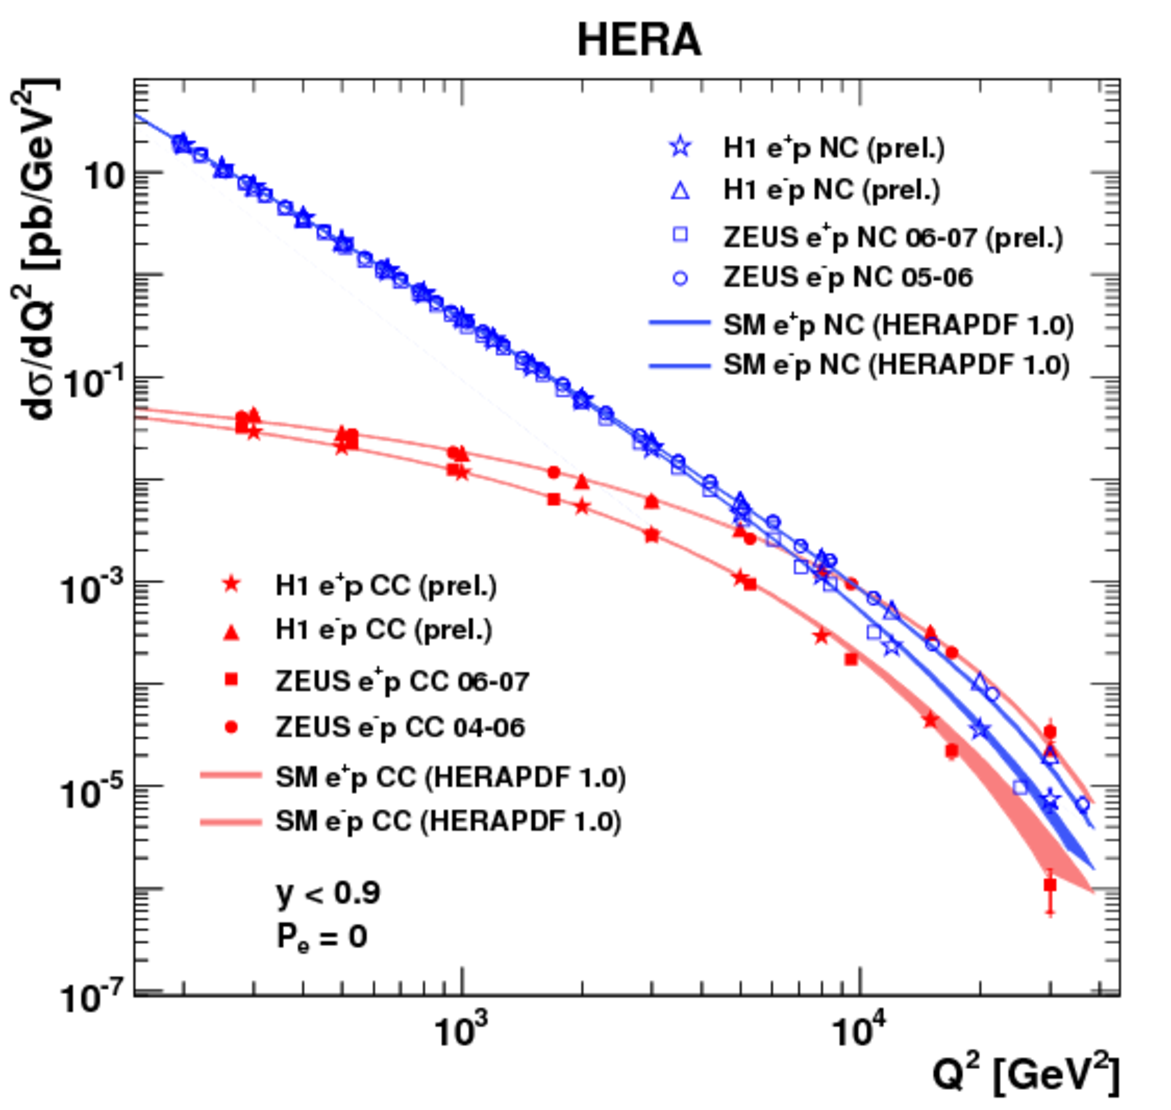
\includegraphics[width=\textwidth]{images/chapter_3/electroweakUnification.pdf}
    \caption[Electroweak unification measurements at HERA]{Neutral current (blue) and charged current (red) differential cross sections as a function of $Q^2$ in $e^\pm p$ collisions, indicating unification at large $Q^2$. \cite{SUSYUnification}}
    \label{fig:ch3_electroweakUnification}
  \end{center}
\end{figure}

\clearpage

\subsection{\texorpdfstring{$\e^+ \e^-$}{EE} colliders}

There have been a multitude of $\e^+ \e^-$ experiments with a centre of mass enery of a few $\gev$ to over $200 \gev$.  There is planning for a linear $\e^+ \e^-$ collider up to $1\tev$.

The charm quark was discovered in 1974 at SLAC (and in a $p \, \textrm{Be}$ experiment at BNL) via the detection of the decay of the bound state, the $J/\psi$ meson.  $m_{J/\psi} \simeq 3.1 \gev$.  A dimuon mass spectrum from the CMS experiment is shown in figure \ref{fig:ch3_mumuspectrumCMS}.

\begin{figure}[!htb]
  \begin{center}
    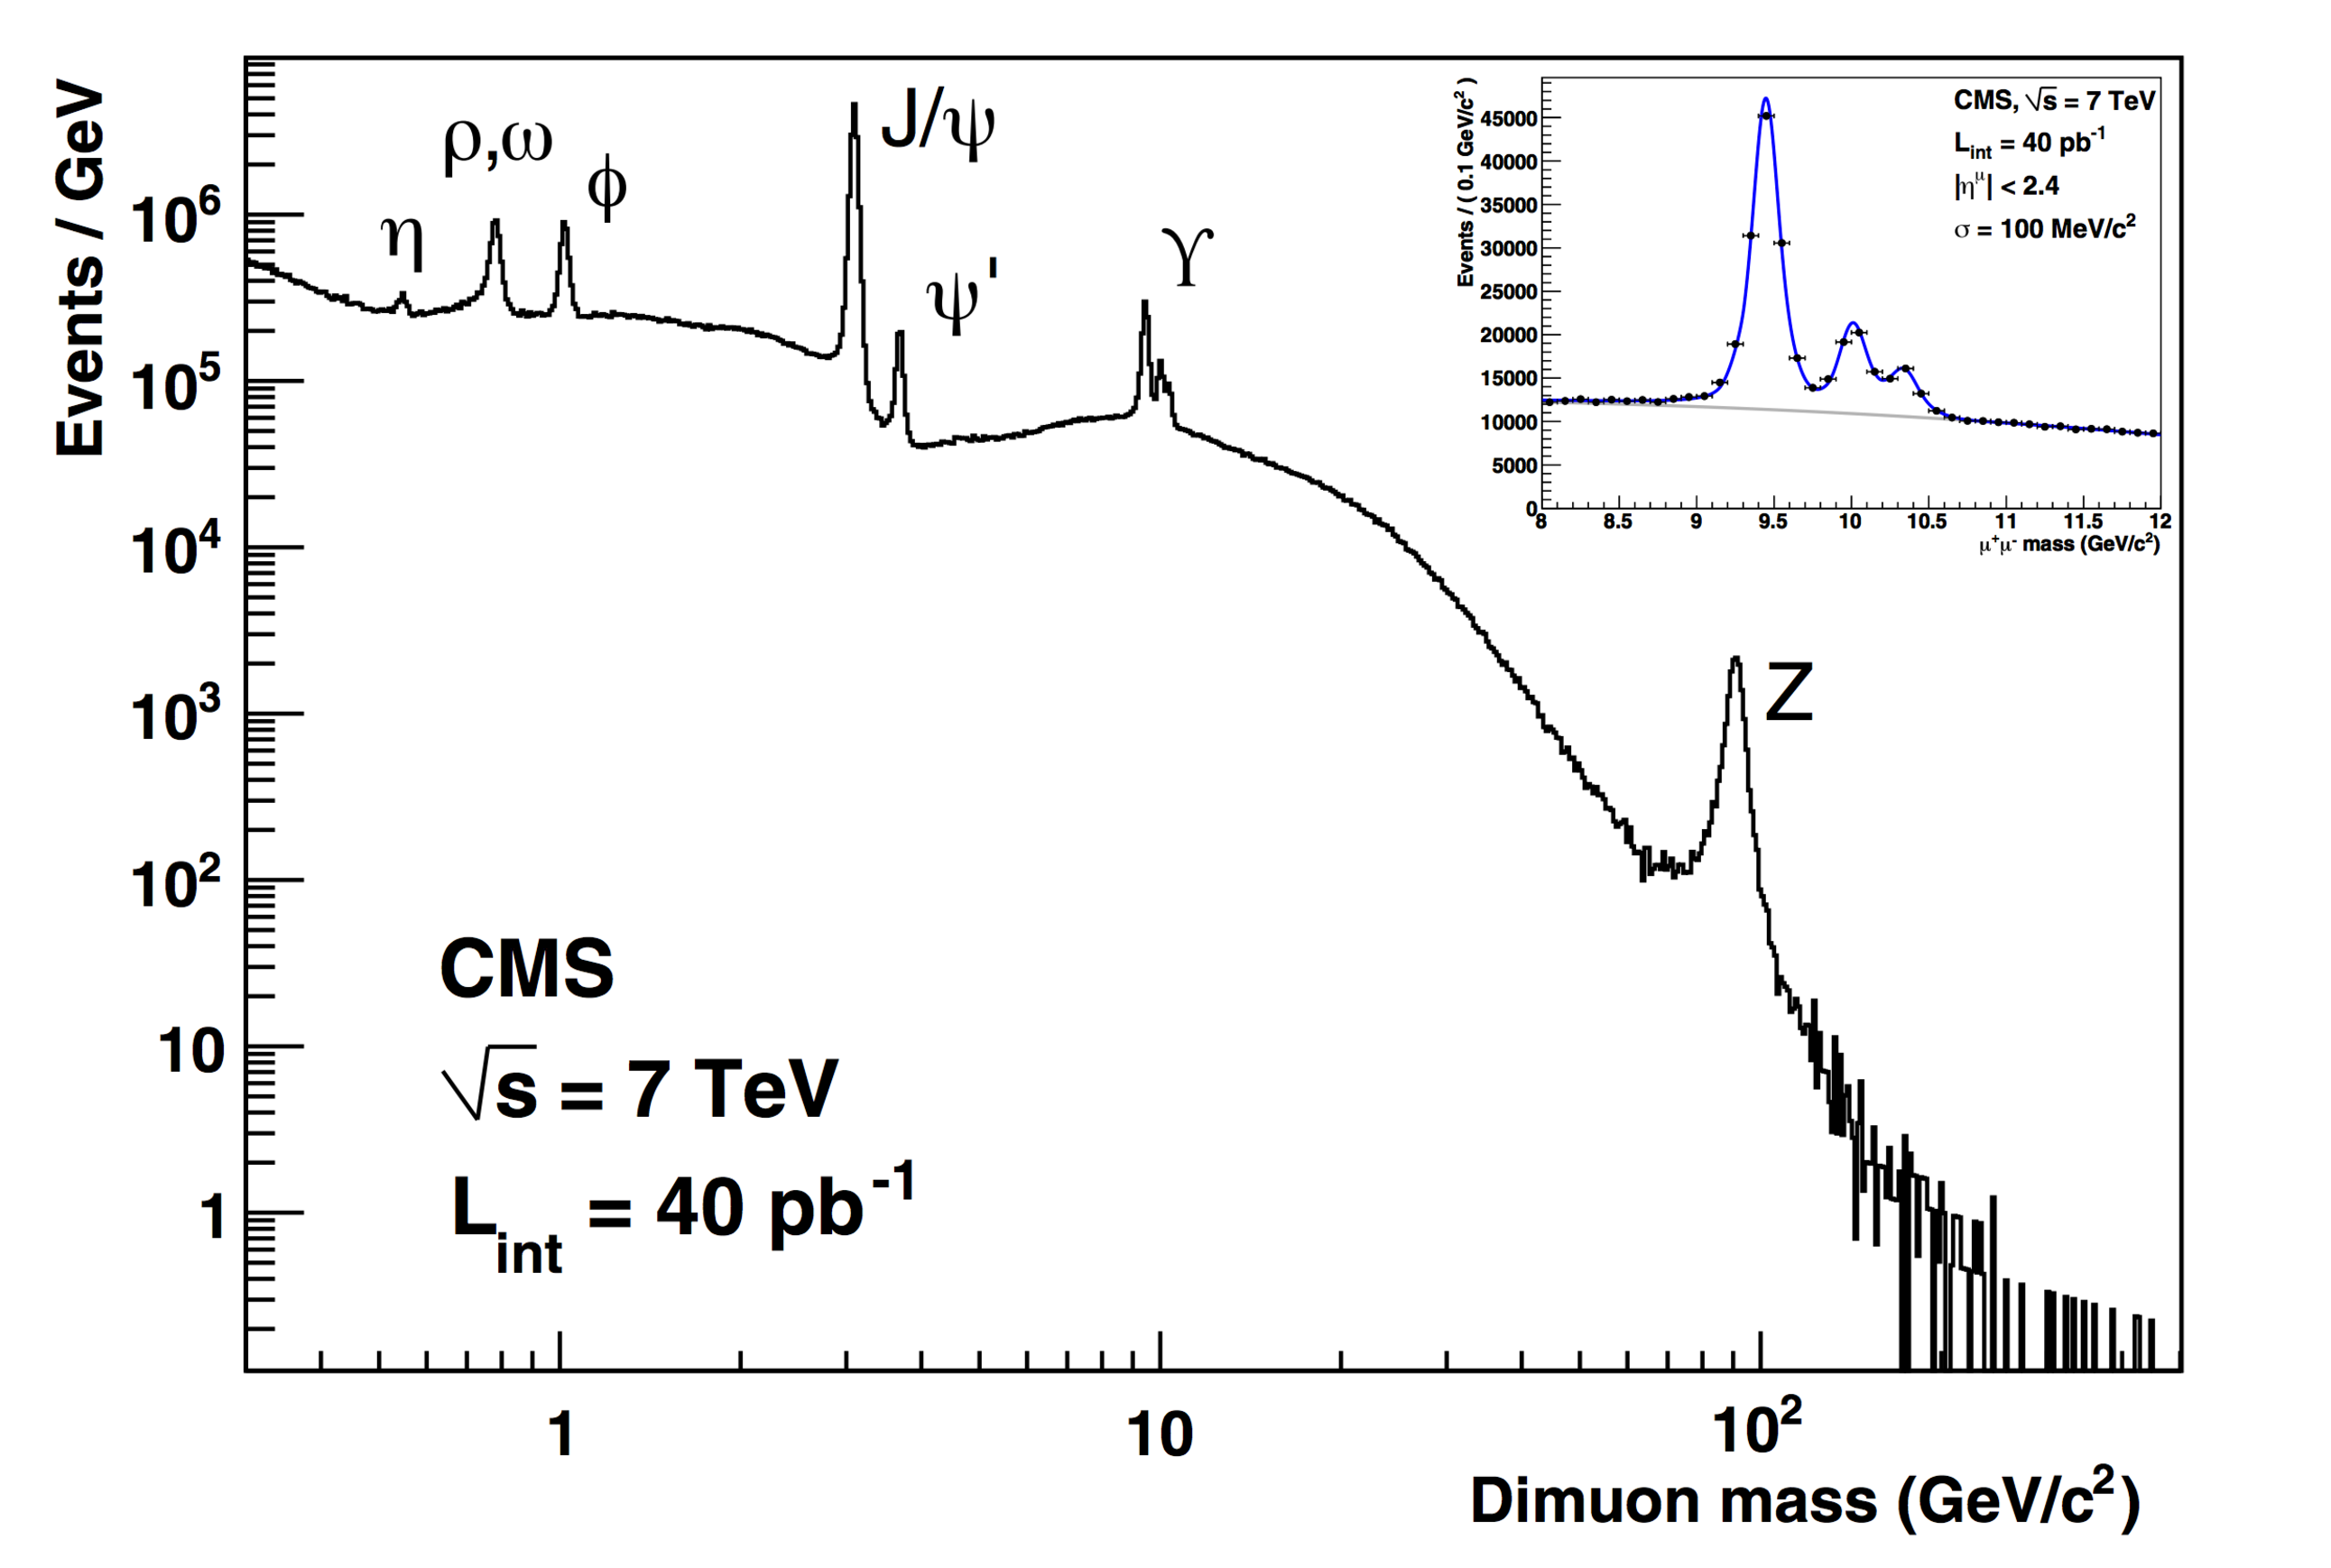
\includegraphics[width=0.9\textwidth]{images/chapter_3/mumuspectrumCMS.pdf}
    \caption[CMS dimuon mass spectrum]{CMS dimuon mass spectrum, over a wide range of masses. \cite{mumuspectrumCMS}}
    \label{fig:ch3_mumuspectrumCMS}
  \end{center}
\end{figure}

In 1979 the gluon was discovered by the experiments at the PETRA collider in DESY at $\sqrt{s} = 35\gev$.  Although $\e^+ \e^-$ is a clean leptonic enviornment, it can provide a powerful probe of QCD eg discovery of the gluon through the oserbvation of $3-$jet events.

Most simply one would expect a srtaightforward process with back to back jets of equal energy.  However, in the detector three jets were seen (one of the quarks radiated a gluon), as indicated in figure \ref{fig:ch3_TwoJetVsThreeJet}.

\begin{figure}[!htb]
  \begin{center}
    \begin{tabular}{c}
      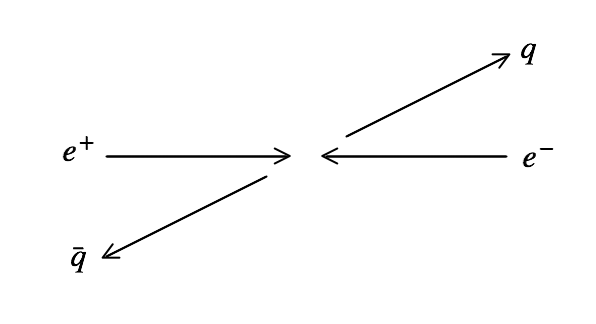
\includegraphics[width=0.6\textwidth]{images/web_feynman/image_14.png} \\
      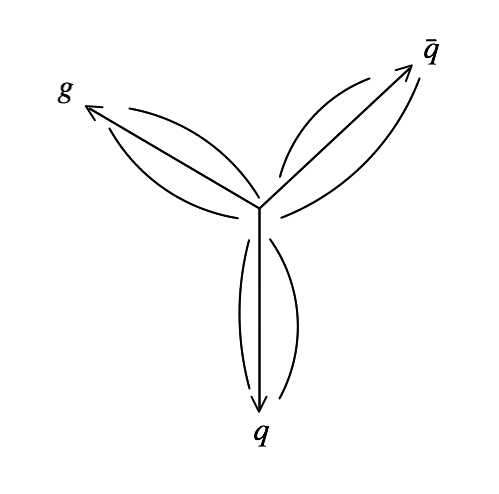
\includegraphics[width=0.6\textwidth]{images/web_feynman/image_15.png}
    \end{tabular}
    \caption[Two and three jet events]{Typical two and three jet events, which were seen at the LEP and HERA experiments.  The Feynman diagrams are shown in the top row and the jet topologies in the transverse plane are shown in the lower row.}
    \label{fig:ch3_TwoJetVsThreeJet}
  \end{center}
\end{figure}

In 1989 the Large Electron-Positron (LEP) collider turned on, embarking on a new era of precision physocs (running at the mass of the $Z^0$ boson.)  Initial LEP running was at the $Z^0$ peak $\simeq 91\gev$, and then moved through $2M_W \simeq 160\gev$ and finally to just over $200 \gev$, looking for the Higgs boson.  There were four multipurpose experiments.  The experiments were most famous for the precision measurements of electroweak parameters such as $M_Z$ and $M_W$.  The measurement of the cross-section as a function of $\sqrt{s}$ was fundamental in measuring $M_Z$ and constraining the number of light neutrinos, as shown in figure \ref{fig:ch3_neutrinos}.

\begin{figure}[!htb]
  \begin{center}
    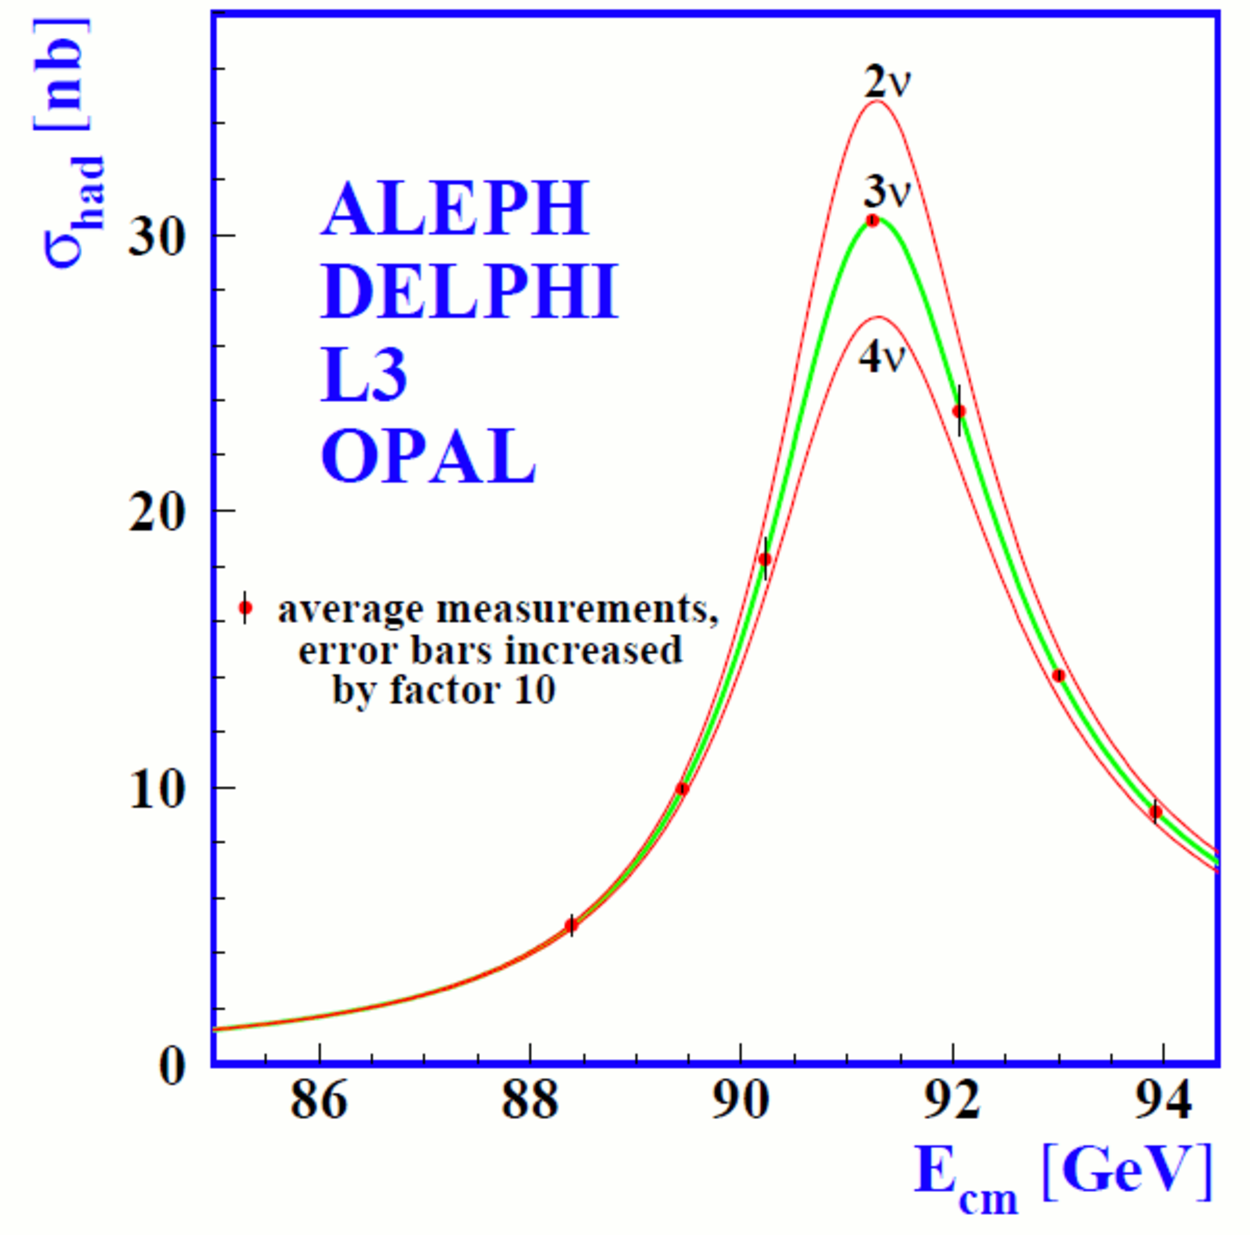
\includegraphics[width=0.8\textwidth]{images/chapter_3/zwidth.pdf}
    \caption[Fit to the number of neutrinos using LEP data]{Fit to the the width of the $Z$ boson to estimate the number of light neutrinos using data from the ALEPH, Delphi, L3 and Opal experiments at LEP. \cite{numberOfNeutrinos}}
    \label{fig:ch3_neutrinos}
  \end{center}
\end{figure}

\begin{eqnarray*}
  M_Z & = 91.1876 & \pm 0.0024 \gev \\
  M_W & = 80.403  & \pm 0.029  \gev
\end{eqnarray*}

In the absence of direct measurements, precise determination of known parameters constrain new physics phenomena eg Higgs boson.  In its final throws LEP also searched for the Higgs boson via Higgstrahlung, where a virtual $Z^0$ results in a real $Z^0$ and Higgs boson.  The process is shown in figure \ref{fig:ch3_EEToHZ}.

\begin{figure}[!htb]
  \begin{center}
    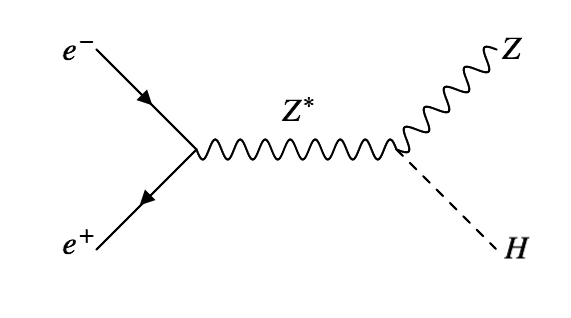
\includegraphics[width=0.8\textwidth]{images/web_feynman/image_16.png}
    \caption[Feynman diagram of $ee\to HZ$]{Feynman diagram showing the process of Higgstrahlung $ee\to HZ$.}
    \label{fig:ch3_EEToHZ}
  \end{center}
\end{figure}

The centre of mass energy was constantly increased as the necessary energy, $E$ had to satisfy $E > M_H + M_Z$, but the Higgs boson was not observed.

Limits of circular $\e^+ \e^-$ machines are being reached due to the rate of energy loss due to synchrotron radiation.

The next planned major collider is the International Linear Collider (ILC).  This would complement the LHC because of the cleanliness of the signal.  This can act as a ``factory'' for eg $t\bar{t}$ production, Higgstrahlung etc.

\subsection{Hadron-hadron colliders}

Due to the hadronic structure and multitude of final states, these colliders are generally more complicated than $\e^+ \e^-$ colliders.  However, they are usually the energy frontier and thereby produce discoveries and measurements of known phenomena over a large kinematic range.

The discovery of the $b$ quark took place in 1977 by obvserving the production and decay of the $\Upsilon$ mesons via $\mu^+ \mu^-$ in $p \quad \textrm{Be}$ collisions at Fermilab.

\begin{figure}[!htb]
  \begin{center}
    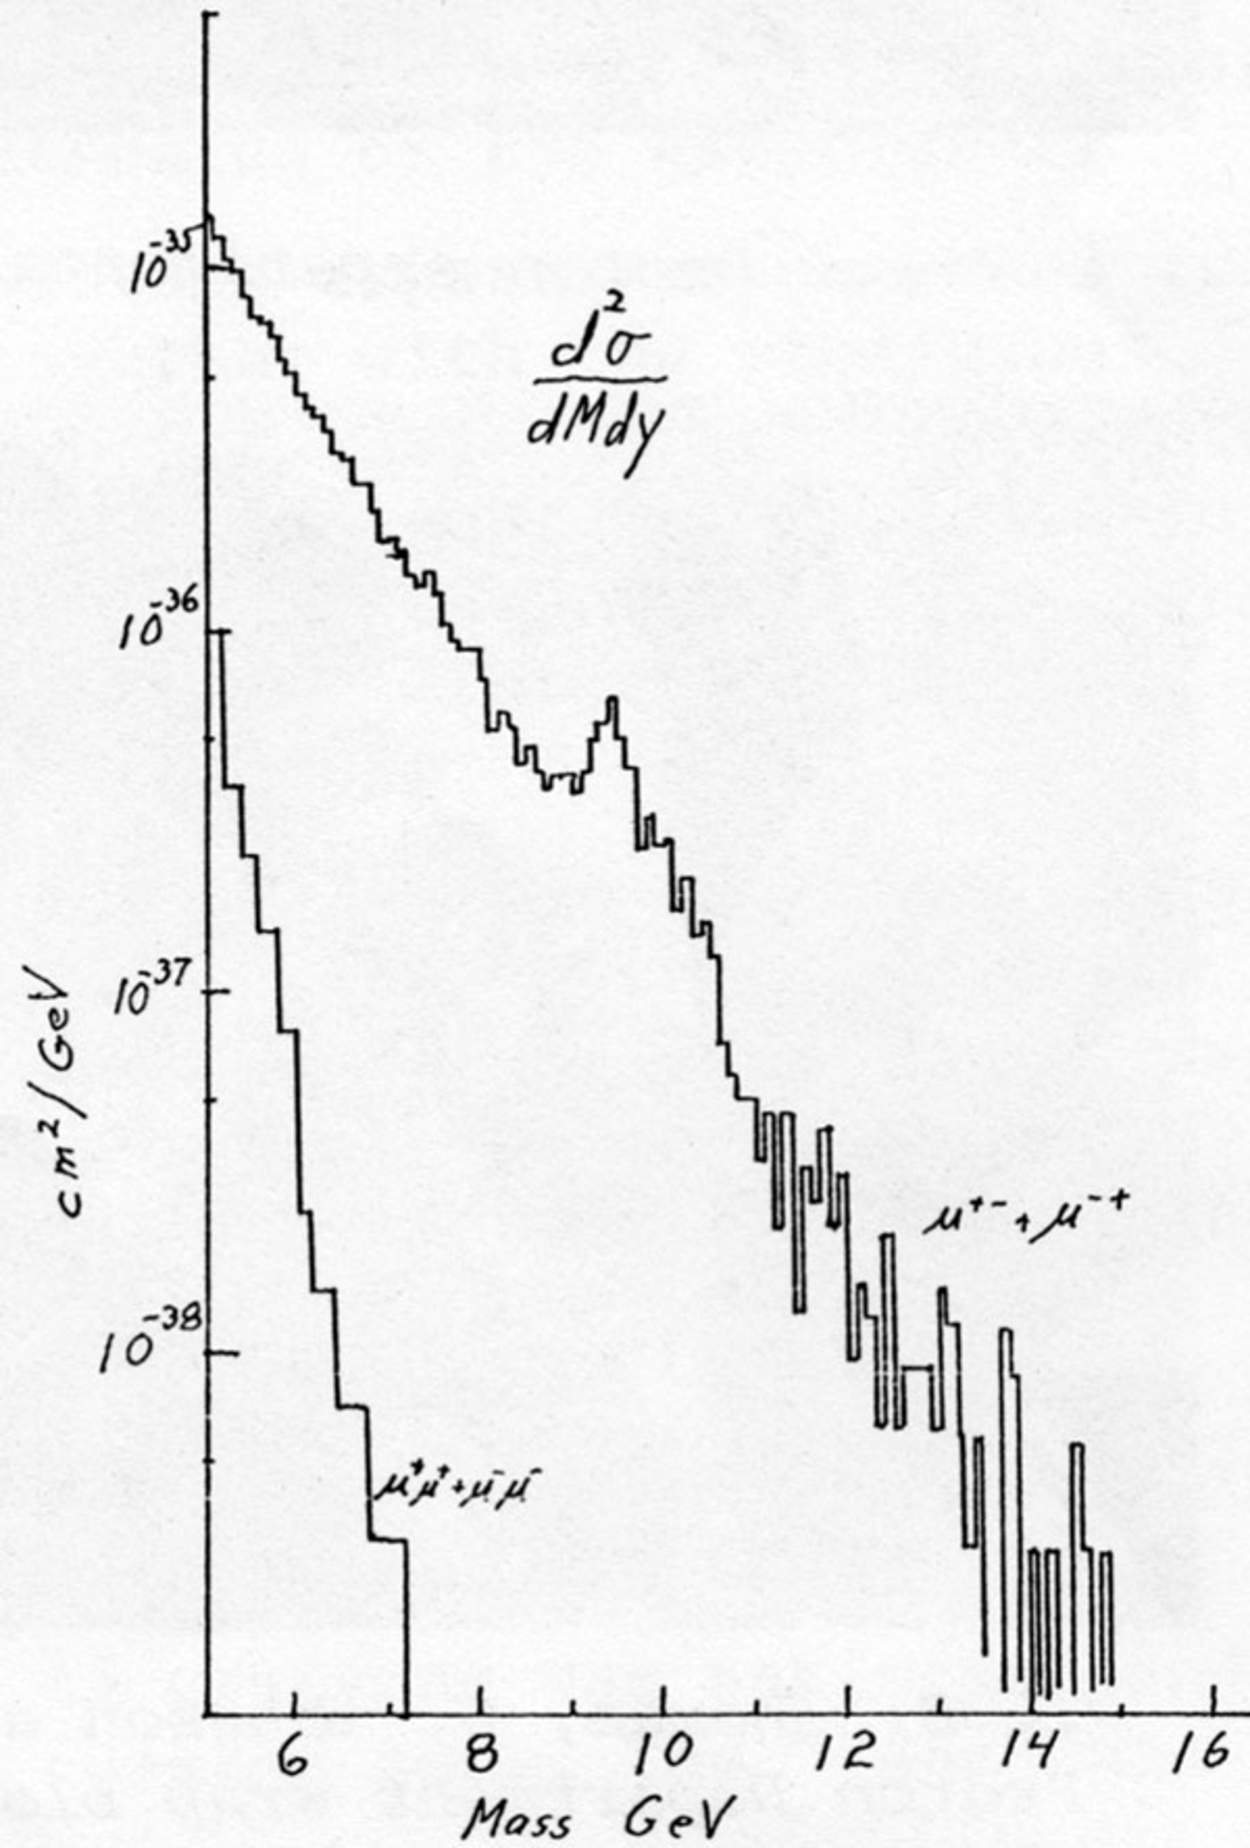
\includegraphics[width=0.75\textwidth]{images/chapter_3/Upsilon.pdf}
    \caption[Discovery of the $\Upsilon(1S)$]{Discovery of the $\Upsilon(1S)$ in the dimuon final state. \cite{Upsilon}}
    \label{fig:ch3_Upsilon}
  \end{center}
\end{figure}

The invariant mass of the $\mu^+ \mu^-$ pair was was observed and a resonance was apparent.

The $W^{\pm}$ and $Z^0$ bosons were discovered in 1984 at the SppS collider at CERN.  Leptonic decays of the $W^{\pm}$ and $Z^0$ were searched for, as they give a lower background relative to hadronic decays ($\sqrt{s} = 540 \gev$).  The top quark was discovered by CDF and D0 at $\sqrt{s} = 1800\gev$ in 1995.

\begin{figure}[!htb]
  \begin{center}
    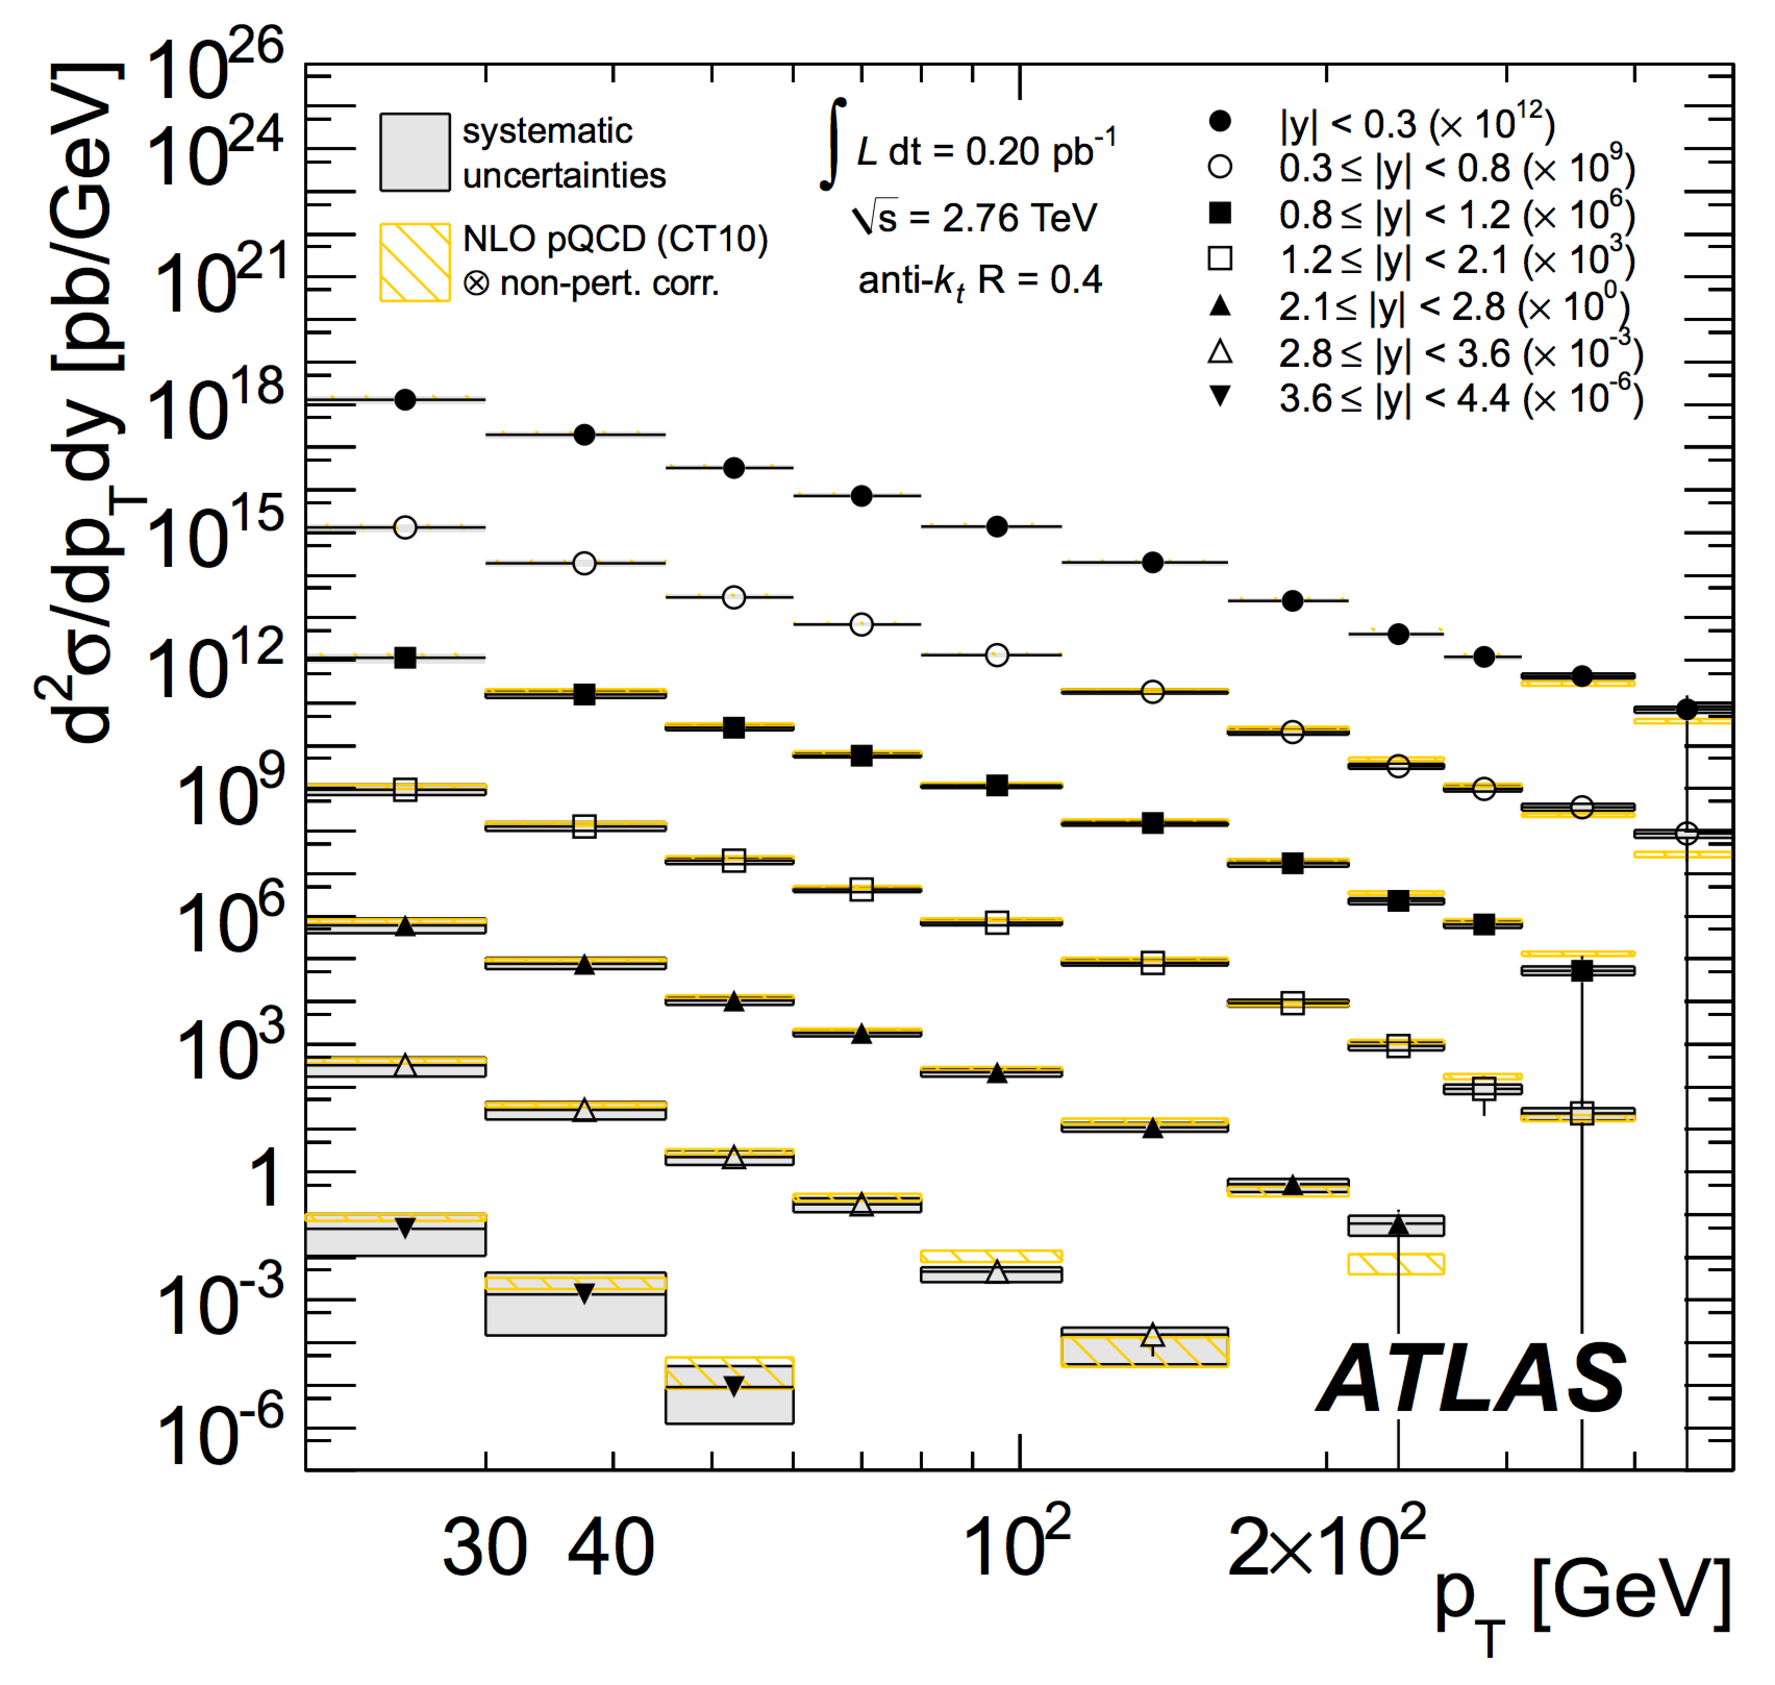
\includegraphics[width=\textwidth]{images/chapter_3/QCD_pt.pdf}
    \caption[Differential cross section of jets]{Differential cross section of jets as function of transverse momentum and pseudorapidity, using data from the ATLAS experiment. \cite{QCD_pt}}
    \label{fig:ch3_QCD_pt}
  \end{center}
\end{figure}

There are high jet energies measures over 24 orders of magnitude in the differential cross-section, as shown in figure \ref{fig:ch3_QCD_pt}.  This allows physicsts to
\begin{itemize}
  \item verify and understand QCD
  \item look for new physics at the highest energies (eg quark substructure)
\end{itemize}
\cleardoublepage
% Copyright Aidan Randle-Conde 2007-2014
% http://www.aidansean.com/phd_notes
% Anyone is free to download, redistribute, edit and use these notes and the source tex files with the following restrictions:
% This 
%  This message is included in the tex source files.
%  Aidan Randle-Conde is credited as the author.
%  Images are correctly credited to their respective authors, as outlined in the references.
%  No part of these notes may be used for commercial purposes.

\chapter{Review of non relativistic quantum mechanics}
\chaptermark{Non-relativistic quantum mechanics}

\section{Schroedinger picture and probability current}

For a free particle of mass $m$ the classical energy-momentum relation is:

\[
  E = \frac{p^2}{2m}
\]

In quantum mechanics, $p$ and $E$ become differential operators:

\begin{eqnarray*}
  E & \to & 1\frac{\partial}{\partial t} \\
  p & \to & -i \nabla \\
  ( \hbar & = & 1 )
\end{eqnarray*}

These operate on the wavefunction:

\begin{eqnarray}
  \frac{(-i)^2}{2m}\nabla^2 \psi & = & i \frac{\partial}{\partial t}\psi \nonumber \\
  \frac{-1}{2m}\nabla^2\psi & = & i\frac{\partial \psi}{\partial t} \label{eq:schroedinger1} \\
  \psi^{\star} \times (\ref{eq:schroedinger1}) :\quad \frac{-1}{2m} \psi^{\star}\nabla^2\psi & = & i\psi^{\star}\frac{\partial \psi}{\partial t} \label{eq:schroedinger2} \\
  \textrm{Complex conjugate of (\ref{eq:schroedinger1}): } \frac{-1}{2m}\nabla^2\psi^{\star} & = & -i\frac{\partial \psi^{\star}}{\partial t} \label{eq:schroedinger3} \\
  \psi \times (\ref{eq:schroedinger3}) :\quad \frac{-1}{2m}\psi\nabla^2\psi^{\star} & = & -i\psi\frac{\partial \psi^{\star}}{\partial t} \label{eq:schroedinger4} \\
  (\ref{eq:schroedinger2}) - (\ref{eq:schroedinger4}) & = & i\left( \psi^{\star}\frac{\partial \psi}{\partial t} + \psi\frac{\partial \psi^{\star}}{\partial t} \right) \nonumber \\
  & = & \frac{-1}{2m}\left(\psi^{\star}\nabla^2\psi - \psi\nabla^2\psi^{\star}\right) \nonumber \\
  \textrm{So } i\left(\psi^{\star}\frac{\partial \psi}{\partial t} + \psi\frac{\partial \psi^{\star}}{\partial t}\right) & = & \frac{-1}{2m}\left(\psi^{\star}\nabla^2\psi - \psi\nabla^2\psi^{\star}\right) \nonumber \\
  \textrm{or } \frac{\partial}{\partial t}\left(\psi^{\star}\psi\right) + \frac{i}{2m}\left(\psi\nabla^2\psi^{\star} - \psi^{\star}\nabla^2\psi \right) & = & 0 \nonumber \\
  \frac{\partial}{\partial t}\left(\psi^{\star}\psi\right) + \frac{i}{2m}\ul{\nabla}\cdot\left(\psi\ul{\nabla}\psi^{\star} - \psi^{\star}\ul{\nabla}\psi\right) & = & 0 \nonumber \\
  \frac{\partial}{\partial t}\int_V\left(\psi^{\star}\psi\right) \mathrm{d}V + \frac{i}{2m}\int_V \ul{\nabla}\cdot\left(\psi\ul{\nabla}\psi^{\star}-\psi\ul{\nabla}\psi\right) \mathrm{d}V & = & 0 \label{eq:schroedinger5}
\end{eqnarray}

(\ref{eq:schroedinger5}) resembles a conservation equation of the form:

\[
  \frac{\partial \rho}{\partial t} + \ul{\nabla}\cdot\ul{J} = 0
\]

where:

\begin{eqnarray*}
  \ul{J} & = & \frac{i}{2m}\left(\psi\ul{\psi}^{\star} - \psi^{\star}\ul{\nabla}\psi\right) \\
  \rho & = & |\psi|^2
\end{eqnarray*}

The divergence theorem then gives:

\[
  \frac{i}{2m}\int_S\left(\psi\ul{\nabla}\psi^{\star} - \psi^{\star}\ul{\nabla}\psi\right)\cdot\ul{\hat{n}}\mathrm{d}S = \frac{i}{2m}\int_V\left(\psi\ul{\nabla}\psi^{\star} - \psi^{\star}\ul{\nabla}\psi\right)\mathrm{d}V
\]

As an example, consider $\rho$ and $\ul{J}$ for a plane quantum wave:

\begin{eqnarray*}
  \psi & = & N\e^{i\left(px - Et\right)} \\
  \rho & = & |\psi|^2 \\
       & = & \psi^{\star}\psi \\
       & = & N\e^{i\left(px - Et\right)}N^{\star}\e^{-i\left(px - Et\right)} \\
       & = & NN^{\star} \\
       & = & |N|^2 \\
  \textrm{So: } \rho & = & |N|^2 \\
  \ul{J} & = & \frac{i}{2m}\left(\psi\ul{\nabla}\psi^{\star} - \psi\ul{\nabla}\psi\right) \\
       & = & \frac{i}{2m}\lbrace N \e^{i\left(px - Et\right)}\ul{\nabla}N^{\star}\e^{-i\left(px - Et\right)}\ul{\nabla}N\e^{i\left(px - Et\right)}\rbrace \\
       & = & \frac{i}{2m}\lbrace NN^{\star}\e^{i\left(px - Et\right)}\e^{iEt}\left(-ip\right)\e^{-ipx}
             - N^{\star}\e^{-i\left(px - Et\right)}N\e^{-iEt}\left(ip\right)\e^{ipx}\rbrace \\
       & = & \frac{i}{2m}\lbrace NN^{\star}\left(-ip\right) - N^{\star}N\left(ip\right)\rbrace \\
       & = & \frac{|N|^2}{2m}p\times 2 \\
       & = & \frac{p}{m}|N|^2
\end{eqnarray*}

In the Schroedinger picture the operators are time independent whereas the wavefunctions are time dependent.  In classical mechanics the ``operators'' (momentum and energy) are time dependent.  The Heisenberg picture gives a formulation which gives time dependent operators.

\section{The Heisenberg picture}

Starting from the Schroedinger equation:

\[
  i\frac{\partial}{\partial t}\psi(\ul{r},t) = H\psi(\ul{r},t)
\]

Also recall that the expectation of an observable, $A$, represented by the operator $\hat{A}$ is given by:

\[
  \langle \hat{A} \rangle = \int \psi^{\star}(\ul{r},t)A\psi(\ul{r},t)\mathrm{d}^3r
\]

Solving the Schroedinger equation:

\begin{eqnarray*}
  i\frac{\partial \psi(\ul{r},t)}{\partial t} & = & H\psi(\ul{r},t) \\
  i\frac{\partial \psi(\ul{r},t)}{\psi(\ul{r},t)} & = & H \partial t \\
  i\int_0^t \frac{\partial \psi(\ul{r},t)}{\psi(\ul{r},t)} & = & \int_0^t H \partial t' \\
  \Rightarrow \ln\lbrack\psi(\ul{r},t)\rbrack - \ln\lbrack\psi(\ul{r},0)\rbrack & = & -iHt \\
  \textrm{So } \frac{\psi(\ul{r},t)}{\psi(\ul{r},0)} & = & \e^{-iHt} \\
  \Rightarrow \psi(\ul{r},t) & = & \psi(\ul{r},0)\e^{-iHt}
\end{eqnarray*}

Condsider the expectation of $A$:

\begin{eqnarray*}
  \langle \hat{A} \rangle & = & \int\psi^{\star}(\ul{r},0)\e^{iHt}\hat{A}\psi(\ul{r},t)\e^{-iHt}\mathrm{d}^3r \\
  \textrm{Define }A_H & = & \e^{iHt}\hat{A}\e^{-iHt} \\
  \frac{\mathrm{d}A_H}{\mathrm{d}t} & = & iH\e^{iHt}\bar{A}\e^{-iHt} + \e^{iHt}\hat{A}(iH)\e^{-iHt} \\
  & = & i(H\hat{A} - \bar{A}H) \\
  & = & i\lbrack H , \hat{A} \rbrack
\end{eqnarray*}

In the interaction picture the time dependent perturbations are given by:

\[
  H = H_0 + H'
\]

where $H_0$ is unperturbed and $H'$ is an interaction perturbation.

\[
  \textrm{Define } H^0_I = \e^{iH_0t}H'\e^{-H_0t}
\]

This gives:

\[
  \frac{\mathrm{d}H'_I}{\mathrm{d}t} = i\lbrack H_0 , H' \rbrack
\]

\section{The harmonic oscillator}

This is a mechanical system which can be used to introduce the concept of creation annihilation operators.

\[
  H = \frac{p^2}{2m} + \frac{1}{2}m\omega^2q^2
\]

The potential energy arises because of a force proportonal to $q$:

\begin{eqnarray*}
  \textrm{Recall } F & = & -kq \\
  & = & m \frac{\mathrm{d}^2q}{\mathrm{d}t^2} \\
  \omega & = & \sqrt{\frac{k}{m}} \\
  V & = & -\int F \mathrm{d}q \\
  & = & \int kq \mathrm{d}q \\
  & = & \frac{kq^2}{2} \\
  k & = & m\omega^2 \\
  \textrm{So } V & = & \frac{m\omega^2q^2}{2}
\end{eqnarray*}

Consider the creation and annihilation operators:

\begin{eqnarray*}
  \textrm{Let } \hat{a} & = & \frac{1}{\sqrt{2}}\left(\sqrt{m\omega}\hat{q} + \frac{i}{\sqrt{m\omega}}\hat{p} \right) \\
  \hat{a}^{\dagger}     & = & \frac{1}{\sqrt{2}}\left(\sqrt{m\omega}\hat{q} - \frac{i}{\sqrt{m\omega}}\hat{p} \right)
\end{eqnarray*}

Consider the commutator given by $\lbrack \hat{q} , \hat{p} \rbrack = i$:

\begin{eqnarray*}
  \lbrack \hat{a} , \hat{a}^{\dagger} \rbrack
  & = & \frac{1}{\sqrt{2}\sqrt{2}}
        \left( m\omega \lbrack \hat{q},\hat{q} \rbrack
        + \frac{i}{\sqrt{m\omega}}\lbrack\hat{p},\hat{q}\rbrack\sqrt{m\omega} \right. \\
  &   & \left. - i\sqrt{m\omega}\lbrack\hat{q},\hat{p}\rbrack\frac{1}{\sqrt{m\omega}}
        + \frac{1}{m\omega}\lbrack\hat{p},\hat{p}\rbrack\right) \\
  & = & \frac{1}{2}\left(i(-i) - i (i) \right) \\
  & = & 1 \\
  \textrm{So } \lbrack \hat{a},\hat{a}^{\dagger}\rbrack & = & 1
\end{eqnarray*}

The Hamiltonian can be written as:

\begin{equation}
  H = \frac{\left(\hat{a}^{\dagger}\hat{a} + \bar{a}\bar{a}^{\dagger}\right)}{2}\omega \label{eq:hamiltonianSHO}
\end{equation}

To demonstrate (\ref{eq:hamiltonianSHO}):

\begin{eqnarray*}
  \hat{a}^{\dagger}\hat{a} & = & \frac{1}{\sqrt{2}}\left(\sqrt{m\omega}\hat{q} - \frac{i}{\sqrt{m\omega}}\hat{p}\right)\frac{1}{\sqrt{2}}\left(\sqrt{m\omega}\hat{q} + \frac{i}{\sqrt{m\omega}}\hat{p}\right) \\
  & = & \frac{1}{2}\left(m\omega\hat{q}^2 + \frac{\hat{p}^2}{m\omega} + 2i\left(\hat{q}\hat{p} - \hat{q}\hat{q}\right)\right) \\
  \hat{a}\hat{a}^{\dagger} & = & \frac{1}{2}\left(m\omega \hat{q}^2 + \frac{\hat{p}^2}{m\omega} + i\left(\hat{p}\hat{q} - \hat{q}\hat{p}\right)\right) \\
  \textrm{So } \hat{a}^{\dagger}\hat{a} + \hat{a}\hat{a}^{\dagger} & = & m\omega \hat{q}^2 + \frac{\hat{p}^2}{m\omega}
\end{eqnarray*}

\begin{eqnarray*}
  \textrm{Recall } H & = & \frac{p^2}{2m} + \frac{m\omega^2q^2}{2} \\
  \textrm{then } H & = & \left( \frac{p^2}{m\omega} + m\omega q^2 \right) \frac{\omega}{2}
\end{eqnarray*}

which leads to (\ref{eq:hamiltonianSHO}).

(\ref{eq:hamiltonianSHO}) may also be written as:

\begin{eqnarray*}
  H & = & \left( \hat{a}^{\dagger} \hat{a} + 1/2 \right)\omega \\
  \textrm{using } \lbrack \hat{a},\hat{a}^{\dagger} \rbrack & = & 1
\end{eqnarray*}

$\hat{a}^{\dagger}$ can be considered as a creation operator:

\begin{eqnarray*}
  \lbrack H,\hat{a} \rbrack & = & \lbrack \left(\hat{a}^{\dagger}\hat{a} + 1/2 \right)\omega , \hat{a} \rbrack \\
  & = & \left(\hat{a}^{\dagger}\hat{a}\hat{a} + \hat{a}\hat{a}^{\dagger}\hat{a} \right)\omega \\
  & = & \lbrack\hat{a}^{\dagger},\hat{a}\rbrack\hat{a}\omega \\
  & = & -\hat{a}\omega \\
  \textrm{Similarly } \lbrack H,\hat{a}^{\dagger}\rbrack & = & \hat{a}^{\dagger} \omega
\end{eqnarray*}

Consider a state $|n\rangle$ such that:

\[
  H|n\rangle = E_n |n\rangle
\]

The energy of $\hat{a}^{\dagger}|n\rangle$ is given by:

\begin{eqnarray*}
  H\hat{a}^{\dagger} |n\rangle & = & \left(\hat{a}^{\dagger}\omega + \hat{a}^{\dagger}H\right)|n\rangle \\
  & = & \left(\hat{a}^{\dagger}\omega + \hat{a}^{\dagger}E_n\right)|n\rangle \\
  & = & \left(E_n + \omega\right)\hat{a}^{\dagger}|n\rangle \\
  \textrm{Similarly } H\hat{a}|n\rangle & = & \left(E_n - \omega\right)\hat{a}|n\rangle
\end{eqnarray*}

So the energy of the state $\hat{a}^{\dagger}|n\rangle$ is $\omega$ greater then that of state $|n\rangle$.  Similarly, the energy of the state $\hat{a}|n\rangle$ is $\omega$ smaller than that of state $|n\rangle$.

There must be a state containing no quantum mechanical oscillations such that:

\[
  \hat{a}|0\rangle = 0
\]

Applying the creation and annihilation operators to the ground state gives:

\begin{eqnarray*}
  \hat{a}^{\dagger}|0\rangle & = & |1\rangle \\
  \frac{\left(\hat{a}^{\dagger}\right)^2}{\sqrt{2}}|0\rangle & = & |2\rangle \\
  \textrm{Generally } |n\rangle & = & \frac{\left(\hat{a}^{\dagger}\right)^n}{\sqrt{n!}}
\end{eqnarray*}

Applying the Hamiltonian operator to the ground state gives:

\begin{eqnarray*}
  H|0\rangle & = & \left(\hat{a}^{\dagger}\hat{a} + 1/2\right)\omega|0\rangle \\
  & = & \frac{\omega}{2}|0\rangle
\end{eqnarray*}

Applying $H$ to $\hat{a}^{\dagger}|0\rangle$ gives:

\begin{eqnarray*}
  H \hat{a}^{\dagger}|0\rangle & = & \left( \hat{a}^{\dagger}\omega + \hat{a}^{\dagger} H\right) |0\rangle \\
  & = & \hat{a}^{\dagger}\left( \omega + H \right) |0\rangle \\
  & = & \hat{a}^{\dagger} \left( \omega + \frac{\omega}{2}\right)|0\rangle \\
  & = & \left(1 + 1/2\right)\omega\hat{a}^{\dagger}|0\rangle
\end{eqnarray*}

Therefore the energy of the system is $\omega$ greater than that of the state $|0\rangle$.  In general:

\begin{eqnarray*}
  H_n\hat{a}^{\dagger}|0\rangle & = & \left(n + 1/2\right)\omega\hat{a}^{\dagger}|0\rangle \\
  \textrm{But }H & = & \left( \hat{a}^{\dagger}\hat{a} + 1/2\right)\omega \\
  \Rightarrow \hat{a}^{\dagger}\hat{a}|0\rangle & = & n|0\rangle
\end{eqnarray*}

So $\hat{a}^{\dagger}\hat{a}$ is the number operator and the energy is given by $E_n = (n + 1/2)\omega$.

The number operator then acts as:

\begin{eqnarray*}
  |n\rangle   & = & \frac{1}{\sqrt{n!}}\left(\hat{a}^{\dagger}\right)^n|0\rangle \\
  |n+1\rangle & = & \frac{1}{\sqrt{(n+1)!}}\left(\hat{a}^{\dagger}\right)^{n+1}|0\rangle \\
              & = & \frac{1}{\sqrt{(n+1)!}}\hat{a}^{\dagger}\left(\hat{a}\right)^n|0\rangle \\
              & = & \frac{1}{\sqrt{(n+1)!}}\hat{a}^{\dagger}\sqrt{n!}|n\rangle \\
  \Rightarrow \hat{a}^{\dagger}|n\rangle & = & \sqrt{n+1}|n+1\rangle \\
  \hat{a}|n\rangle & = & \sqrt{n}|n-1\rangle
\end{eqnarray*}

It is now possible to conceive of a primitive field theory which can create or annihilate quanta of the appropriate field eg electromagnetism.

\section{The anharmonic oscillator}

This model will describe how to put interactions into a field theory.  An interaction will move quanta from a state to higher or lower states.

For the anharmonic oscillator:

\begin{eqnarray*}
  H & = & \frac{p^2}{2m} + \frac{m\omega^2 x^2}{2} + \lambda x^3 \\
    & = & H_0 + \lambda H'
\end{eqnarray*}

\subsection{Rayleigh-Schroedinger perturbation theory}

\begin{eqnarray*}
  H & = & H_0 + \lambda H' \\
  \textrm{where } H_0 |n\rangle^0 & = & E^0_n|n\rangle^0 \\
  E_n & = & E^0_n + \lambda E^1_n + \lambda^2 E^2_n + \cdots \\
  \textrm{and } |n\rangle & = & |n\rangle^0 + \lambda|n\rangle^1 + \lambda|n\rangle^2 + \cdots
\end{eqnarray*}

Note that $|n\rangle^1$, $|n\rangle^2$ etc are orthogonal to $|n\rangle^0$.

\begin{eqnarray*}
  \textrm{Since } H & = & H_0 + \lambda H': \\
  H|n\rangle        & = & \left(H_0 + \lambda H_1\right)\left(|n\rangle^0 + \lambda|n\rangle^1 + \lambda^2|n\rangle^2\right) \\
                    & = & E|n\rangle \\
                    & = & \left(E^0_n + \lambda E^1_n + \lambda^2 E^2_n\right)\left( |n\rangle^0 + \lambda |n\rangle^1 + \lambda^2|n\rangle^2 \right) \\
\end{eqnarray*}

\begin{eqnarray*}
  \lambda^0 \textrm{ terms: } & H_0|n\rangle^0 & = E^0_n|n\rangle \\
  \lambda^1 \textrm{ terms: } & H_0|n\rangle^1 - E^0_n|n\rangle^1 + H_1|n\rangle^0 - E_n^1|n\rangle^0 & = 0 \\
\end{eqnarray*}
\[
  \textrm{ie } \left( H_0 -E^0_n \right) |n\rangle^1 + \left( H^1 - E^1_n \right) |n \rangle^0 = 0
\]

Premultiplying by $^0\langle n | :$

\begin{eqnarray*}
  ^0\langle n | H_0 - E_n^0 |n\rangle^1 + ^0\langle n | H^1 - E^1_n|n\rangle^0 & = & 0 \\
  \Rightarrow ^0\langle n|H^1 - E^1_n|n\rangle & = & 0 \\
  \Rightarrow \langle E^1_n\rangle & = & ^0\langle n | H^1 |n\rangle^0
\end{eqnarray*}

Premultiplying the expression for $\lambda^1$ terms by $^0\langle m|$ (orthogonal to $|n\rangle^0$):

\begin{eqnarray*}
  ^0\langle m|H_0|n\rangle^1 - ^0\langle m|E^0_n|n\rangle^1 + ^0\langle m|H^1|n\rangle^0 - ^0\langle m|E^1_n|n|\rangle^0 & = & 0 \\
  \Rightarrow ^0\langle m|E^0_m-E^1_n|n\rangle^1 + ^0\langle m|H^1|n\rangle^0 - {^0\langle m|n\rangle^0}E^1_n & = & 0 \\
  \textrm{So } ^0\langle m|E^0_m-E^0_n|n\rangle^1 + ^0\langle m|H^2|n\rangle^0 & = & 0 \\
  \textrm{So } ^0\langle n\rangle^1 & = & \frac{^0\langle m|H^1|n\rangle^0}{E^0_m - E^0_n}
\end{eqnarray*}

\begin{eqnarray*}
  \textrm{Therefore } |n\rangle & = & |n\rangle^0 + \lambda|n\rangle^1 + \cdots \\
  & = & |n\rangle^0 + \lambda \sum_m |m \rangle^0 \frac{^0\langle m|H^1|n\rangle^0}{E^0_m - E^0_n}
\end{eqnarray*}

using the identity:

\[
  |n\rangle^1 = \displaystyle\sum_m |m\rangle^0 {}^0\langle m|n\rangle^1
\]

Calculating the value of $\lambda x^3$:

\begin{eqnarray*}
  \hat{a} & = & \sqrt{\frac{m\omega}{2}}\hat{q} - \frac{i}{\sqrt{2m\omega}}\hat{p} \\
  \hat{a}^{\dagger} & = & \sqrt{\frac{m\omega}{2}}\hat{q} + \frac{i}{\sqrt{2m\omega}}\hat{p} \\
  \left(\hat{a} + \hat{a}^{\dagger}\right) & = & \sqrt{2m\omega}\hat{q} \\
  \textrm{So } \hat{q} & = & \frac{1}{\sqrt{2m\omega}}\left(\hat{a} + \hat{a}^{\dagger}\right) \\
  \hat{q}^3 & = & \frac{1}{\left(2m\omega\right)^{3/2}}\left(\hat{a} + \hat{a}^{\dagger}\right)^3
\end{eqnarray*}

So the term becomes:

\[
  \frac{\lambda}{\left(2m\omega\right)^{3/2}}\displaystyle\sum_m |m\rangle^0 \frac{^0\langle m|\left( \hat{a} + \hat{a}^{\dagger}\right)^3|n\rangle^0}{E^0_m - E^0_n}
\]

Looking at $^0\langle m|\left(\hat{a} + \hat{a}^{\dagger}\right)|n\rangle^0$:

\begin{eqnarray*}
  ^0\langle m|\left(\hat{a} + \hat{a}^{\dagger}\right)|n\rangle^0 & = & ^0\langle m|\left(\hat{a} + \hat{a}^{\dagger}\right)^2\left(\hat{a} + \hat{a}^{\dagger}\right)|n\rangle^0 \\
  & = & ^0\langle m|\left(\hat{a}^2 + \hat{a}\hat{a}^{\dagger} + \hat{a}^{\dagger}\hat{a}+\hat{a}^{\dagger 2}\right)\left(\hat{a} + \hat{a}^{\dagger}\right)|n\rangle^0
\end{eqnarray*}

using $\lbrack \bar{a},\bar{a}^{\dagger}\rbrack = 1$ and $\bar{a}^{\dagger}\bar{a} = n$

\begin{eqnarray*}
  \textrm{Also: }\hat{a}^{\dagger}|n\rangle & = & \sqrt{n + 1}|n + 1\rangle \\
  & = & \sqrt{n} |n - 1 \rangle
\end{eqnarray*}

\begin{eqnarray*}
  \lambda x^3 & = ^0\langle m| \lbrack & \sqrt{n(n-1)(n-2)}|n-3\rangle^0 \\
              &                        & + \sqrt{(n+1)(n+2)(n+3)}|n+3\rangle^0 \\
              &                        & + (3+2n)\sqrt{n}|n-1\rangle^0 \\
              &                        & + (1+3n)\sqrt{n+1}|n+1\rangle^0
                   \rbrack
\end{eqnarray*}

\section{The Lagrangian}

Physical systems evolve such that the action:

\[
  s = \int L(q,\dot{q})\mathrm{d}t
\]

is extremised (usually minimised.) ie the system follows a path from $t_1$ to $t_2$ such that the integral of the Lagrangian over $t$ is minimised, as shown in figure \ref{fig:ch4_action}.  This is an alternative formulation of classical mechanics eg Newton's law:

\[
  F = \frac{\mathrm{d}}{\mathrm{d}t}\left(mv\right)
\]

\begin{figure}[!htb]
  \begin{center}
    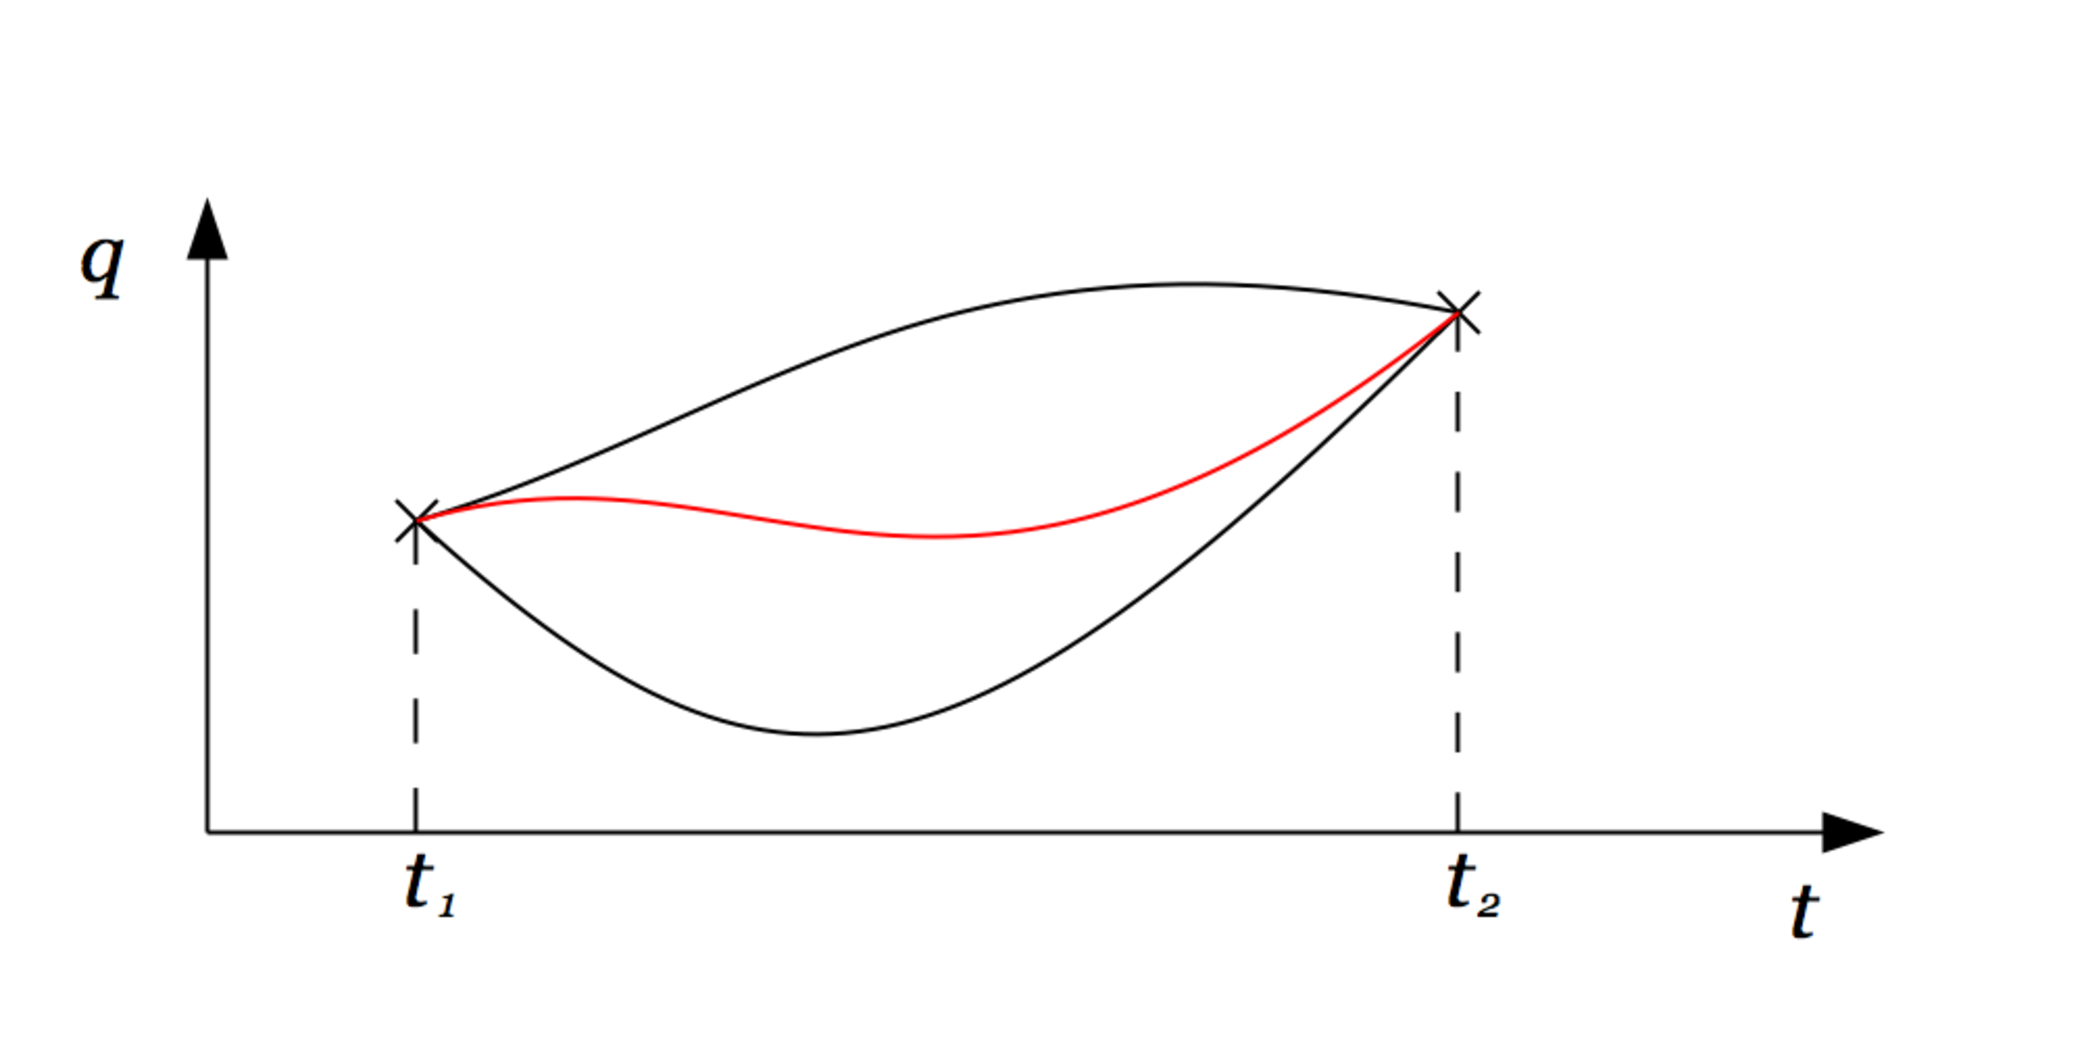
\includegraphics[width=\textwidth]{images/chapter_4/action2.pdf}
    \caption[Schematic diagram showing action]{In general several paths connect points $(x_1;t_1)$ and $(x_2;t_2)$, but the path which minimises the action is favoured.  The red path indicates the path which minimises action.}
    \label{fig:ch4_action}
  \end{center}
\end{figure}

\begin{eqnarray*}
  \textrm{If }                s & = & \int_{t_1}^{t_2}L(q,\dot{q})\mathrm{d}t \\
  \textrm{then }       \delta s & = & \int_{t_1}^{t_2}\left( \frac{\partial L}{\partial q}\delta q + \frac{\partial L}{\partial \dot{q}}\delta \dot{q}\right) \mathrm{d}t \\
  \textrm{Now }  \delta \dot{q} & = & \delta \frac{\mathrm{d}q}{\mathrm{d}t} = \frac{\mathrm{d}}{\mathrm{d}t}\left( \delta q \right) \\
  \textrm{So }         \delta s & = & \int_{t_1}^{t_2}\Bigg[ \frac{\partial L}{\partial q}\delta q + \frac{\partial L}{\partial \dot{q}}\frac{\mathrm{d}}{\mathrm{d}t}\left(\delta q \right)\Bigg] \mathrm{d}t
\end{eqnarray*}

Integration by parts gives:

\begin{eqnarray*}
  \delta s & = & \int_{t_1}^{t_2}\Bigg[ \frac{\partial L}{\partial q}\delta q + - \frac{\mathrm{d}}{\mathrm{d}t}\frac{\partial L}{\partial \dot{q}}\delta q \Bigg] \mathrm{d}t + \Bigg[ \frac{\partial L}{\partial \dot{q}}\Bigg]_{t_1}^{t_2} \\
  & = & 0 \\
  \textrm{But } \delta q(t_2) = \delta q(t_1) & = & 0 \\
  \Rightarrow \frac{\partial L}{\partial q} \delta q - \frac{\mathrm{d}}{\mathrm{d}t}\frac{\partial L}{\partial \dot{q}}\delta q & = & 0 \\
  \textrm{or } \frac{\partial L}{\partial q} - \frac{\mathrm{d}}{\mathrm{d}t}\frac{\partial L}{\partial \dot{q}} & = & \textrm{ (The Euler-Lagrange equation)}
\end{eqnarray*}

For the harmonic oscillator:

\begin{eqnarray*}
  L & = & \frac{m\dot{q}^2}{2} - \frac{m\omega^2q^2}{2} \\
  \frac{\partial L}{\partial \dot{q}} & = & m\dot{q} \\
  \frac{\partial L}{\partial q} & = & m\omega^2q \\
  \frac{\mathrm{d}}{\mathrm{d}t}\frac{\partial L}{\partial \dot{q}} = \frac{\partial L}{\partial q} \\
  \Rightarrow m\ddot{q} & = & m\omega^2q
\end{eqnarray*}

giving Newton's second law.

In quantum mechanics, dynamical variables (eg momentum) are operators, and in general do not commute.

\[
  \mathrm{Specifically}\quad \lbrack \hat{q},\hat{p} \rbrack = i
\]

where $\hat{p}$ is the generalisation:

\[
  \hat{p} = \frac{\partial L}{\partial \dot{q}}
\]

The Heisenberg equation of motion for an operator $\hat{A}$ is:

\[
  \frac{\mathrm{d}\hat{A}}{\mathrm{d}t} = i \lbrack H,\hat{A}\rbrack
\]

The Hamiltonian, defined in terms of the Lagrangian is:

\[
  H = \hat{p}\cdot\hat{\dot{q}} - L
\]

In the classical operator:

\begin{eqnarray*}
  L & = & \frac{m\hat{\dot{q}^2}}{2} - \frac{m\omega^2\hat{q}^2}{2} \\
  \frac{\partial L}{\partial \hat{\dot{q}}} & = & \hat{p} \\
  \textrm{So } H & = & \hat{p}\hat{q} - L \\
  & = & \hat{p}\hat{q} - \frac{m\hat{\dot{q}}^2}{2} + \frac{m\omega^2\hat{q}^2}{2} \\
  & = & \hat{p}\frac{\hat{p}}{m} - \frac{\hat{p}^2}{2m} + \frac{m\omega^2}{2}\hat{q}^2 \\
  \textrm{So } H & = & \frac{\hat{p}^2}{2m} + \frac{m\omega^2}{2}\hat{q}^2
\end{eqnarray*}

\subsection{The Dirac \texorpdfstring{$\delta$}{Delta} function}

The Dirac $\delta$ function may be thought of as a function of height $1/\Delta x$ and width $\Delta x$ around a value of $x = x_0$ in the limit $\Delta x \to 0$, as shown in figure \ref{fig:ch4_diracDelta}.

\begin{figure}[!htb]
  \begin{center}
    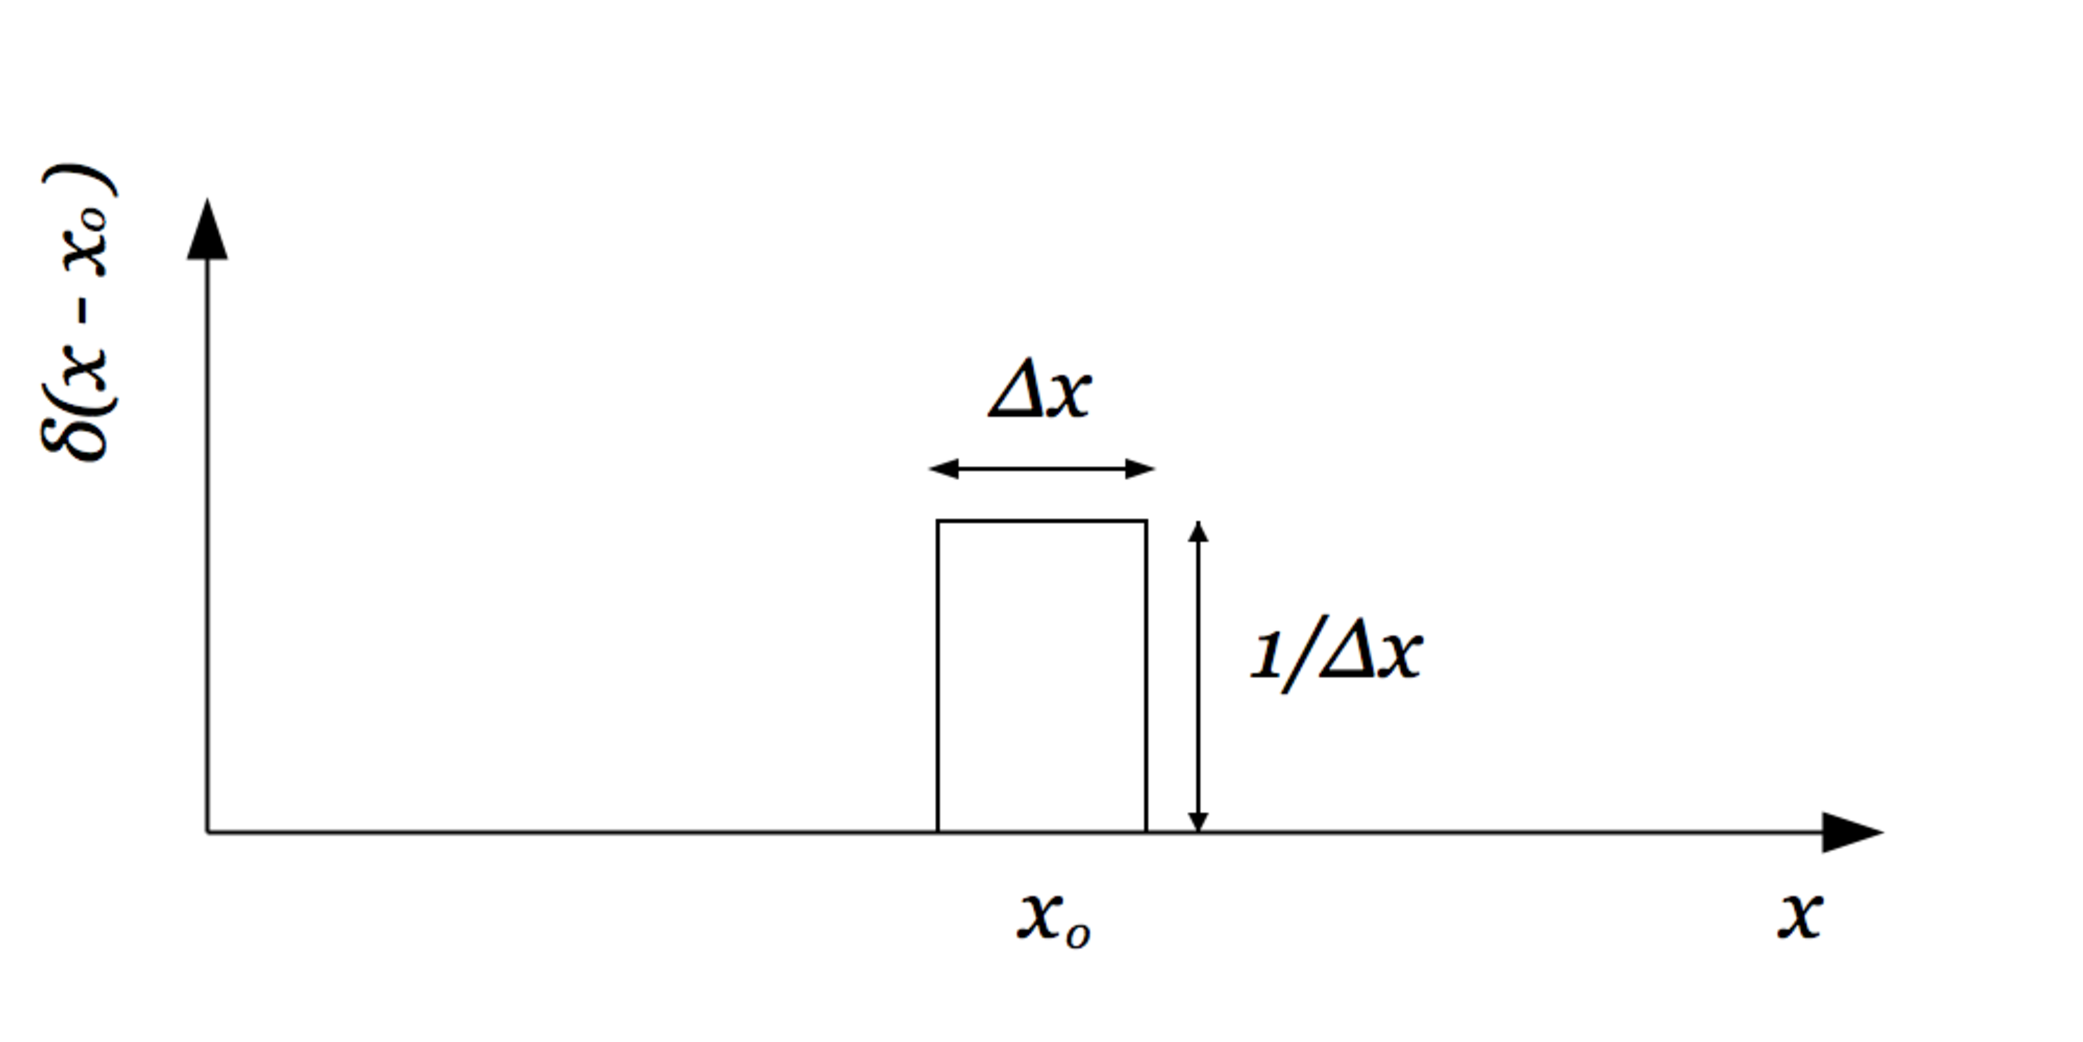
\includegraphics[width=\textwidth]{images/chapter_4/diracDelta.pdf}
    \caption[The Dirac $\delta$ function]{The Dirac $\delta$ function has width $\Delta x$ and height $1/\Delta x$ in the limit $\Delta x\to 0$.}
    \label{fig:ch4_diracDelta}
  \end{center}
\end{figure}

\[
  Area = \int \delta(x - x_0) \mathrm{d}x = 1 \\
\]

\[
  \delta(x-x_0) =
  \Bigg\{
    \begin{array}{cc}
    0 & x\neq x_0 \\
    1 & x = 0
    \end{array}{}
\]

Consider the function $f(x)$ to be split into elements $\Delta x$ wide:

\begin{eqnarray*}
  \int f(x) \mathrm{d}x & =  & \displaystyle\sum_i f(x_i) \Delta x \\
  \int f(x) \delta(x-x_0) \mathrm{d}x & = & \displaystyle\sum_i f(x_i)\delta(x_i - x_0)
\end{eqnarray*}

For the bin $x_i \neq x_0$ it is clear that $\delta(x_i - x_0) = 0$, but when $x_i = x_0$, $\delta(x_i - x_0) = 1/\Delta x$.

\begin{eqnarray*}
  \Rightarrow \int f(x)\delta(x-x_0)\mathrm{d}x & = & \lim_{x \to 0} f(x_0) \frac{1}{\Delta x}\Delta x \\
  \Rightarrow \int f(x)\delta(x-x_0)\mathrm{d}x & = & f(x_0)
\end{eqnarray*}

Some useful expressions and functions limit to the Dirac $\delta$ function:

\begin{eqnarray*}
  \delta(x) = & \displaystyle\lim_{\epsilon \to 0} \frac{1}{\epsilon} & \mathrm{ for } -\epsilon/2 < x < \epsilon/2 \\
  \delta(x) = & \displaystyle\lim_{\epsilon \to 0} \frac{1}{\pi}\frac{\epsilon}{x^2 + \epsilon^2} & \textrm{ (Breit-Wigner resonance)}
\end{eqnarray*}

Consider the Breit-Wigner resonance:

\begin{eqnarray*}
  I & = & \int_{-\infty}^{\infty} \frac{1}{\pi}\frac{\epsilon}{x^2 + \epsilon^2}\mathrm{d}x \\
  x & = & \epsilon \tan \theta \\
  \mathrm{d}x & = & \epsilon \sec^2\theta \\
  I & = & \frac{1}{\pi}\int_{\pi/2}^{\pi/2}\frac{\epsilon\epsilon\sec^2\theta}{\epsilon^2(1 + \tan^2\theta)}\mathrm{d}\theta \\
    & = & 1
\end{eqnarray*}

So it appears that the Breit-Wigner function approaches the Dirac $\delta$ function in the appropriate limit.  At $x=0$ the function has a value $1/\pi\epsilon$.  At $x=\pm\epsilon$ the function reaches the half maximum, $1/2\pi\epsilon$.  $\Gamma/2 = \epsilon$ where $\Gamma$ is the full width at half height and is more commonly used in the Breit-Wigner function.

Another form of the Dirac $\delta$ function is:

\[
  \delta(x-x_0) = \int_{-\infty}^{\infty} \frac{1}{2\pi} \e^{ik(x-x_0)} \mathrm{d}k
\]

Consider Fourier analysis of the above form.  Recall that for a well behaved function of $x$ between $-L/2$ and $L/2$ the function can be expressed as a Fourier series with wavelengths $\lambda = L$, $\frac{L}{2}$, $\frac{L}{3} \cdots$

\[
  f(x) = \displaystyle\sum^{\infty}_{x=-\infty}a_n\e^{i2\pi nx/L}
\]

To find $a_n$ integrate both sides:

\begin{eqnarray*}
  \int_{-L/2}^{L/2}\mathrm{d}xf(x)\e^{-12\pi nx/L} & = & \int_{L/2}^{L/2}a_n \mathrm{d}x \\
  \Rightarrow a_n & = & \frac{1}{L} \int_{-L/2}^{L/2}\mathrm{d}xf(x) \e^{-12\pi nx/L} \\
  \mathrm{Consider } \lim L\to \infty \\
  f(x) & = & \displaystyle\sum_{-\infty}^{\infty}a_n \e^{i2\pi nx/L}\Delta n \\
\end{eqnarray*}

where $\Delta n$ is the interval and $\Delta n = 1$

\begin{eqnarray*}
  \textrm{Define } k & = & \frac{2\pi n}{L} \\
  \mathrm{d}k & = & 2\pi \frac{\Delta n}{L} \\
  f(x) & = & \displaystyle\sum_{-\infty}^{\infty} a_n \e^{ikx} \frac{L}{2\pi} \mathrm{d}k \\
  & = & \frac{1}{2\pi} \int_{-\infty}^{\infty}\e^{ikx}g(k)\mathrm{d}k \\
  \textrm{where } g(k) & = & La_n \\
  g(k) & = & \int_{-\infty}^{\infty} f(x)\e^{-ikx} \mathrm{d}x \\
  f(x) & = & \frac{1}{2 \pi}\int_{-\infty}^{\infty} g(k)\e^{ikx}\mathrm{d}k
\end{eqnarray*}

Substituting $g(k)$ into the expression for $f(x)$:

\begin{eqnarray*}
  f(x) & = & \frac{1}{2 \pi} \int_{-\infty}^{\infty} \int_{-\infty}^{\infty}f(x')\e^{-ikx'}\e^{ikx}\mathrm{d}k\mathrm{d}x' \\
  & = & \int_{-\infty}^{\infty} f(x')\mathrm{d}x' \int_{-\infty}^{\infty} \frac{1}{2\pi} \e^{ik(x-x')}\mathrm{d}k \\
  \textrm{So } \delta(x-x') & = & \frac{1}{2 \pi} \int_{-\infty}^{\infty}\e^{ik(x-x')}\mathrm{d}k
\end{eqnarray*}

Some properties of the Dirac $\delta$ function: \nopagebreak

\begin{enumerate}
\item$\delta(ax) = \delta(x)/a$ Proof:

\begin{eqnarray*}
  \textrm{Let } ax & = & y \\
  \Rightarrow a\mathrm{d}x & = & \mathrm{d} y \\
  \textrm{So } \int_{-\infty}^{\infty}\delta(ax)\mathrm{d}x & = & \int_{-\infty}^{\infty} \delta(y)\frac{\mathrm{d}y}{a} \\
  & = & \frac{1}{a}
\end{eqnarray*}

\item $\delta(x) = \delta(-x) \Rightarrow \delta(x)$ is an even function.

\item$f(x)$ and $f'(x)$  For a function $f(x)$:

\[
  \delta(f(x)) = \displaystyle\sum_i \frac{\delta(x-a_i)}{\left(\frac{\mathrm{d}f}{\mathrm{d}x}\right)_{x=a_i}} \\
\]

where $a_i$ satisfy $f(a_i) = 0$
  
At each place where $f(x) = 0$, then:

\begin{eqnarray*}
  f(x) & = & f(a_i) + (x - a_i)\frac{\mathrm{d}f}{\mathrm{d}x} + \cdots \\
  f(a_i) & = & 0
\end{eqnarray*}

So the $\delta$ function has non-zero contributions from each of the roots $a_i$ of the form:

\begin{eqnarray*}
  \delta(f(x)) & = & \displaystyle\sum_i \delta \left( (x-a_i) \left(\frac{\mathrm{d}f}{\mathrm{d}x}\right)_{x=a_i}\right) \\
  & = & \displaystyle\sum_i \frac{\delta(x-a_i)}{\left(\frac{\mathrm{d}f}{\mathrm{d}x}\right)_{x=a_i}}
\end{eqnarray*}
\end{enumerate}

\subsection{The Heaviside step function}

The Heaviside step function is shown in figure \ref{fig:ch4_heaviside}.  It is defined as:

\begin{figure}[!htb]
  \begin{center}
    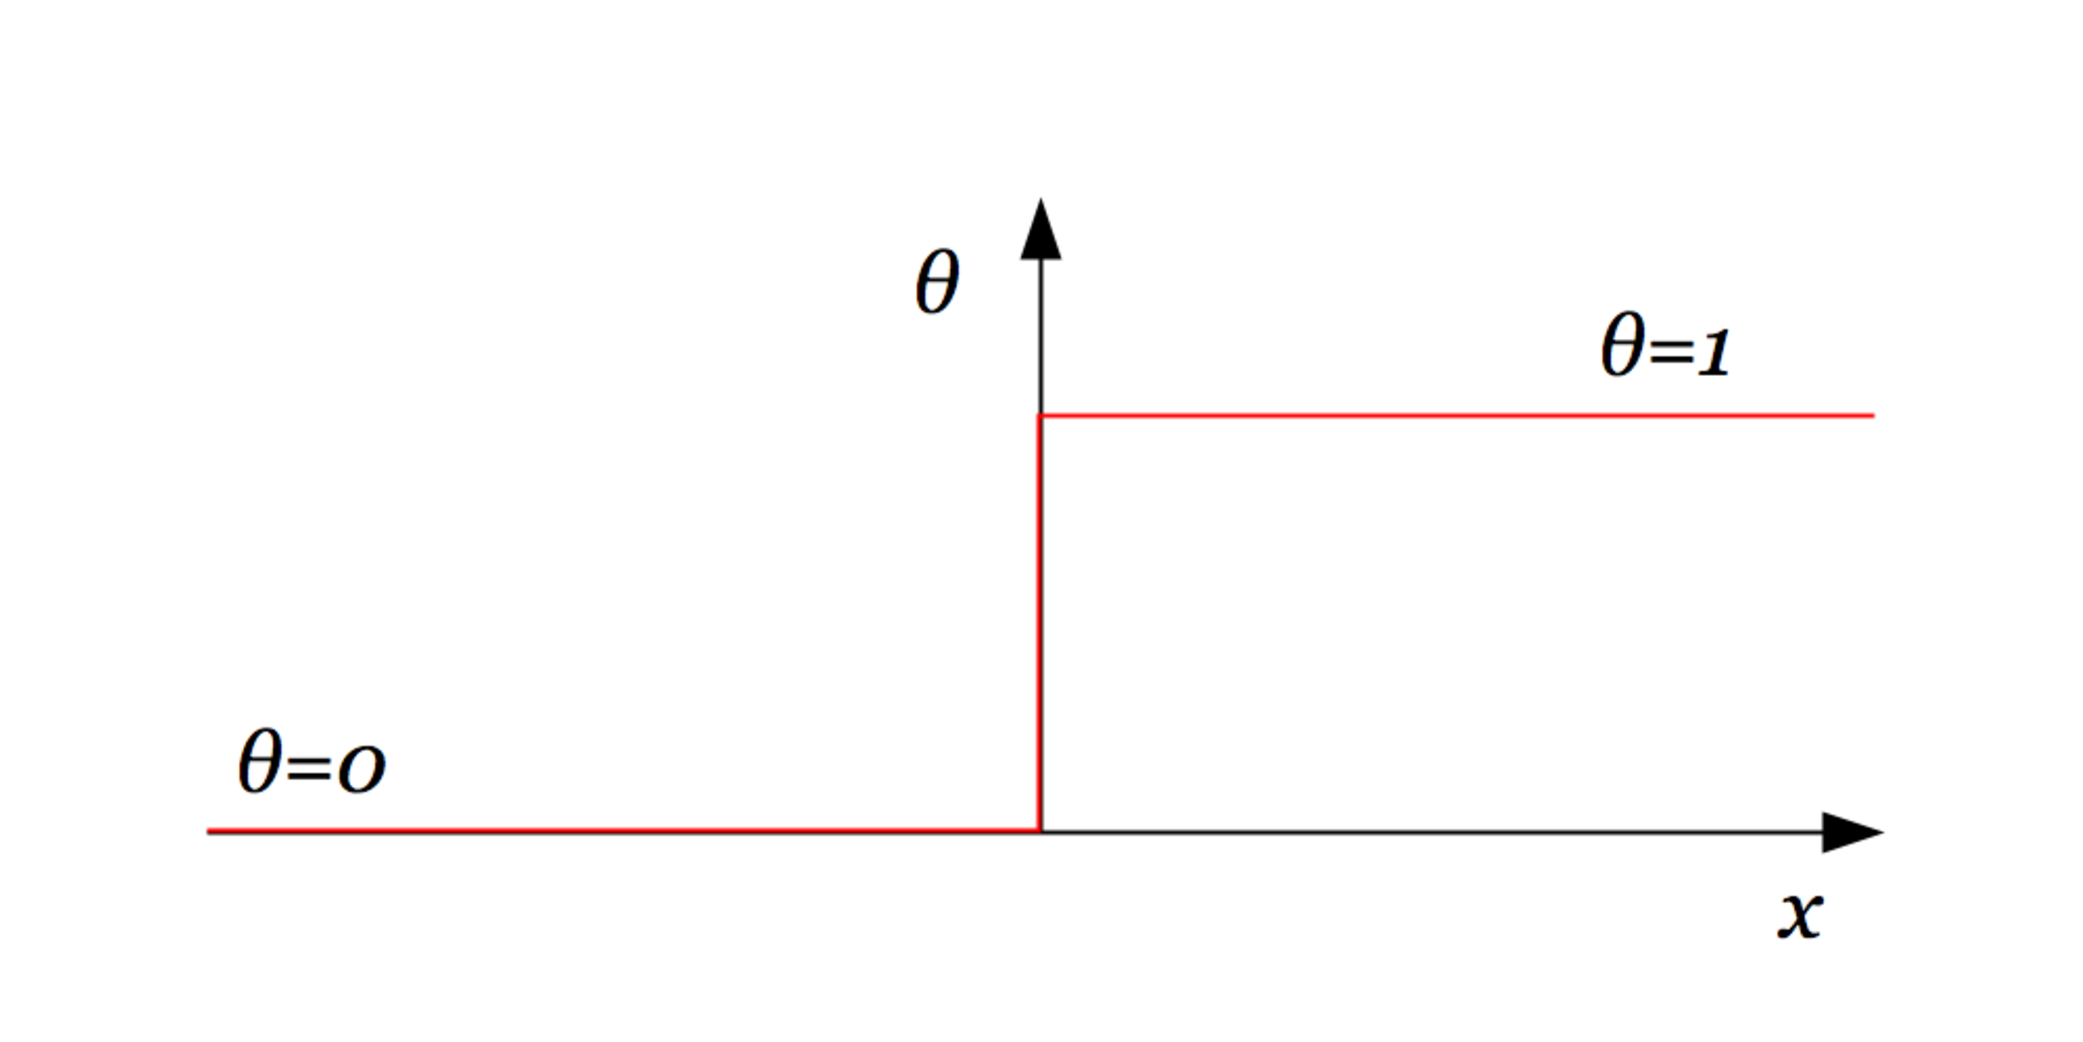
\includegraphics[width=\textwidth]{images/chapter_4/heaviside.pdf}
    \caption[The Heaviside step function]{The Heaviside step function is zero when $x<0$ and unity when $x\ge 0$.}
    \label{fig:ch4_heaviside}
  \end{center}
\end{figure}

\begin{eqnarray*}
  \theta(\tau) & = &
  \left\{
    \begin{array}{cc}
    1 & \tau>0 \\
    0 & \tau<0
    \end{array}
  \right.
  \\
  \frac{\mathrm{d}\theta}{\mathrm{d}\tau} & = & \delta (\tau) \\
  & = & \frac{1}{2\pi} \int_{-\infty}^{\infty}\e^{-i\omega\tau}\mathrm{d}\omega \\
  \Rightarrow \theta & = & \frac{1}{2\pi}\int_{-\infty}^{\infty}\int_{-\infty}{\infty}\e^{-i\omega\tau}\mathrm{d}\omega \mathrm{d}\tau \\
  & = & \frac{1}{2\pi} \int_{-\infty}^{\infty} \frac{\e^{-i\omega\tau}}{-i\omega}\mathrm{d}\omega \\
  \theta & = & \frac{-1}{2\pi i}\int_{-\infty}^{\infty} \frac{\e^{-\omega\tau}\mathrm{d}\omega}{\omega + i\epsilon} \\
\end{eqnarray*}

Using Cauchy's theorem gives:

\begin{eqnarray*}
  \oint_C \frac{f(z)\mathrm{d}z}{z-a} & = & 2\pi i f(a) \\
  \textrm{So } \theta & = & \frac{-1}{2\pi i} \left(-2ni\e^{(-i\tau)(-i\epsilon)}\right) \\
  & = & \e^{-\epsilon\tau} \\
  \textrm{For } \epsilon \to 0, \theta & = & 1
\end{eqnarray*}

\cleardoublepage
% Copyright Aidan Randle-Conde 2007-2014
% http://www.aidansean.com/phd_notes
% Anyone is free to download, redistribute, edit and use these notes and the source tex files with the following restrictions:
% This 
%  This message is included in the tex source files.
%  Aidan Randle-Conde is credited as the author.
%  Images are correctly credited to their respective authors, as outlined in the references.
%  No part of these notes may be used for commercial purposes.

\chapter{Relativity}

An understanding of special relativity is necessary to properly understand much of particle physics.  Four vectors are defined by:

\[
  \begin{array}{ccccccc}
  x^{\mu} & = & (t,\ul{r}) & \quad & x_{\mu} & = & (t,-\ul{r}) \\
  p^{\mu} & = & (E,\ul{p}) & \quad & p_{\mu} & = & (E,-\ul{p}) 
  \end{array}
\]

Scalar products are given by:

\[
  \begin{array}{ccccccc}
  \ul{x}\cdot\ul{x} & = & x^{\mu}x_{\mu} & = & t^2 - x^2 &   & \\
  \ul{p}\cdot\ul{p} & = & p^{\mu}p_{\mu} & = & E^2 - p^2 & = & m^2
  \end{array}
\]

Also $x_{\mu} = g_{\mu\nu}x^{\nu}$, $x^{\nu} = g^{\nu\mu}x_{\mu}$.

where:

\begin{eqnarray*}
  g_{\mu\nu} & = &
  \left(
    \begin{array}{cccc}
    1 &  0 &  0 & 0 \\
    0 & -1 &  0 & 0 \\
    0 &  0 & -1 & 0 \\
    0 &  0 &  0 & -1
    \end{array}
  \right)
  \\
  g_{\mu\nu}g^{\mu\nu} & = & \displaystyle\sum_{\mu} \displaystyle\sum_{\nu} g_{\mu\nu}g^{\mu\nu} \\
  & = & \displaystyle\sum_{\mu}g_{\mu\mu}g^{\mu\mu} \\
  & = & \displaystyle\sum_{\mu}g_{\mu\mu}^2 \\
  & = & 4
\end{eqnarray*}

Recall that from quantum mechanics:

\[
  \begin{array}{ccc}
  E = i\frac{\partial}{\partial t} & \quad & \ul{p} = -i \ul{\nabla}
  \end{array}
\]

\begin{eqnarray*}
  \textrm{But } p^{\mu} = (E,\ul{p}) \\
  & = & i\left( \frac{\partial}{\partial t},-\ul{\nabla}\right) \\
  \textrm{So } p^{\mu} & = & i\partial^{\mu} \\
  \textrm{where } \partial^{\mu} & = & \left(\frac{\partial}{\partial t},-\ul{\nabla}\right) \\
  & = & \frac{\partial}{\partial x_{\mu}} \\
  \textrm{and } \partial_{\mu} & = & \left( \frac{\partial}{\partial t}, \ul{\nabla}\right) \\
  & = & \frac{\partial}{\partial x^{\mu}}
\end{eqnarray*}

Forming the De L'ambertian operator:

\[
  \partial^{\mu}\partial_{\mu} = \Box^2 = \left(\frac{\partial^2}{\partial t^2}, -\nabla^2\right)
\]

\section{Lorentz transformations}

A Lorentz transformation relates the coordinates in one frame to the coordinates of another frame.  By convention the lorentz transformation takes place along the (mutually parallel) $x$ axis, with velocity $v$.  $x'$ tranforms as:

\begin{eqnarray*}
  t'   & = & \gamma (t - vx_1)  \\
  x'_1 & = & \gamma (-vt + x_1) \\
  x'_2 & = & x_2 \\
  x'_3 & = & x_3 \\
  \gamma & = & \frac{1}{\sqrt{1-v^2}}
\end{eqnarray*}

The product $p^{\mu}q_{\mu}$ is invariant under a Lorentz transformation.

\section{The light cone}

Let $x^{\mu}$ denote the four vector $(x^0,\ul{x})$ and suppose light is emitted at $y^{\mu} = (y^0,\ul{y})$.  Consider the difference between $x^{\mu}$ and $y^{\mu}$:

\[
  s^2 = (x^{\mu} - y^{\mu})^2 = (x_0 - y_0)^2 - (\ul{x} - \ul{y})^2
\]

If the above is zero then:

\[
  (x^0 - y^0) = (\ul{x} - \ul{y})^2
\]

This is the equation of a light beam and defines a light cone.  If $s^2>0$ then the separation is time-like and the events are in the forward light cone and causally related.  If $s^2<0$ then the separation is space-like and the events have no causal connection.  The light cone is shown in figure \ref{fig:ch5_lightcone}.

\begin{figure}[!htb]
  \begin{center}
    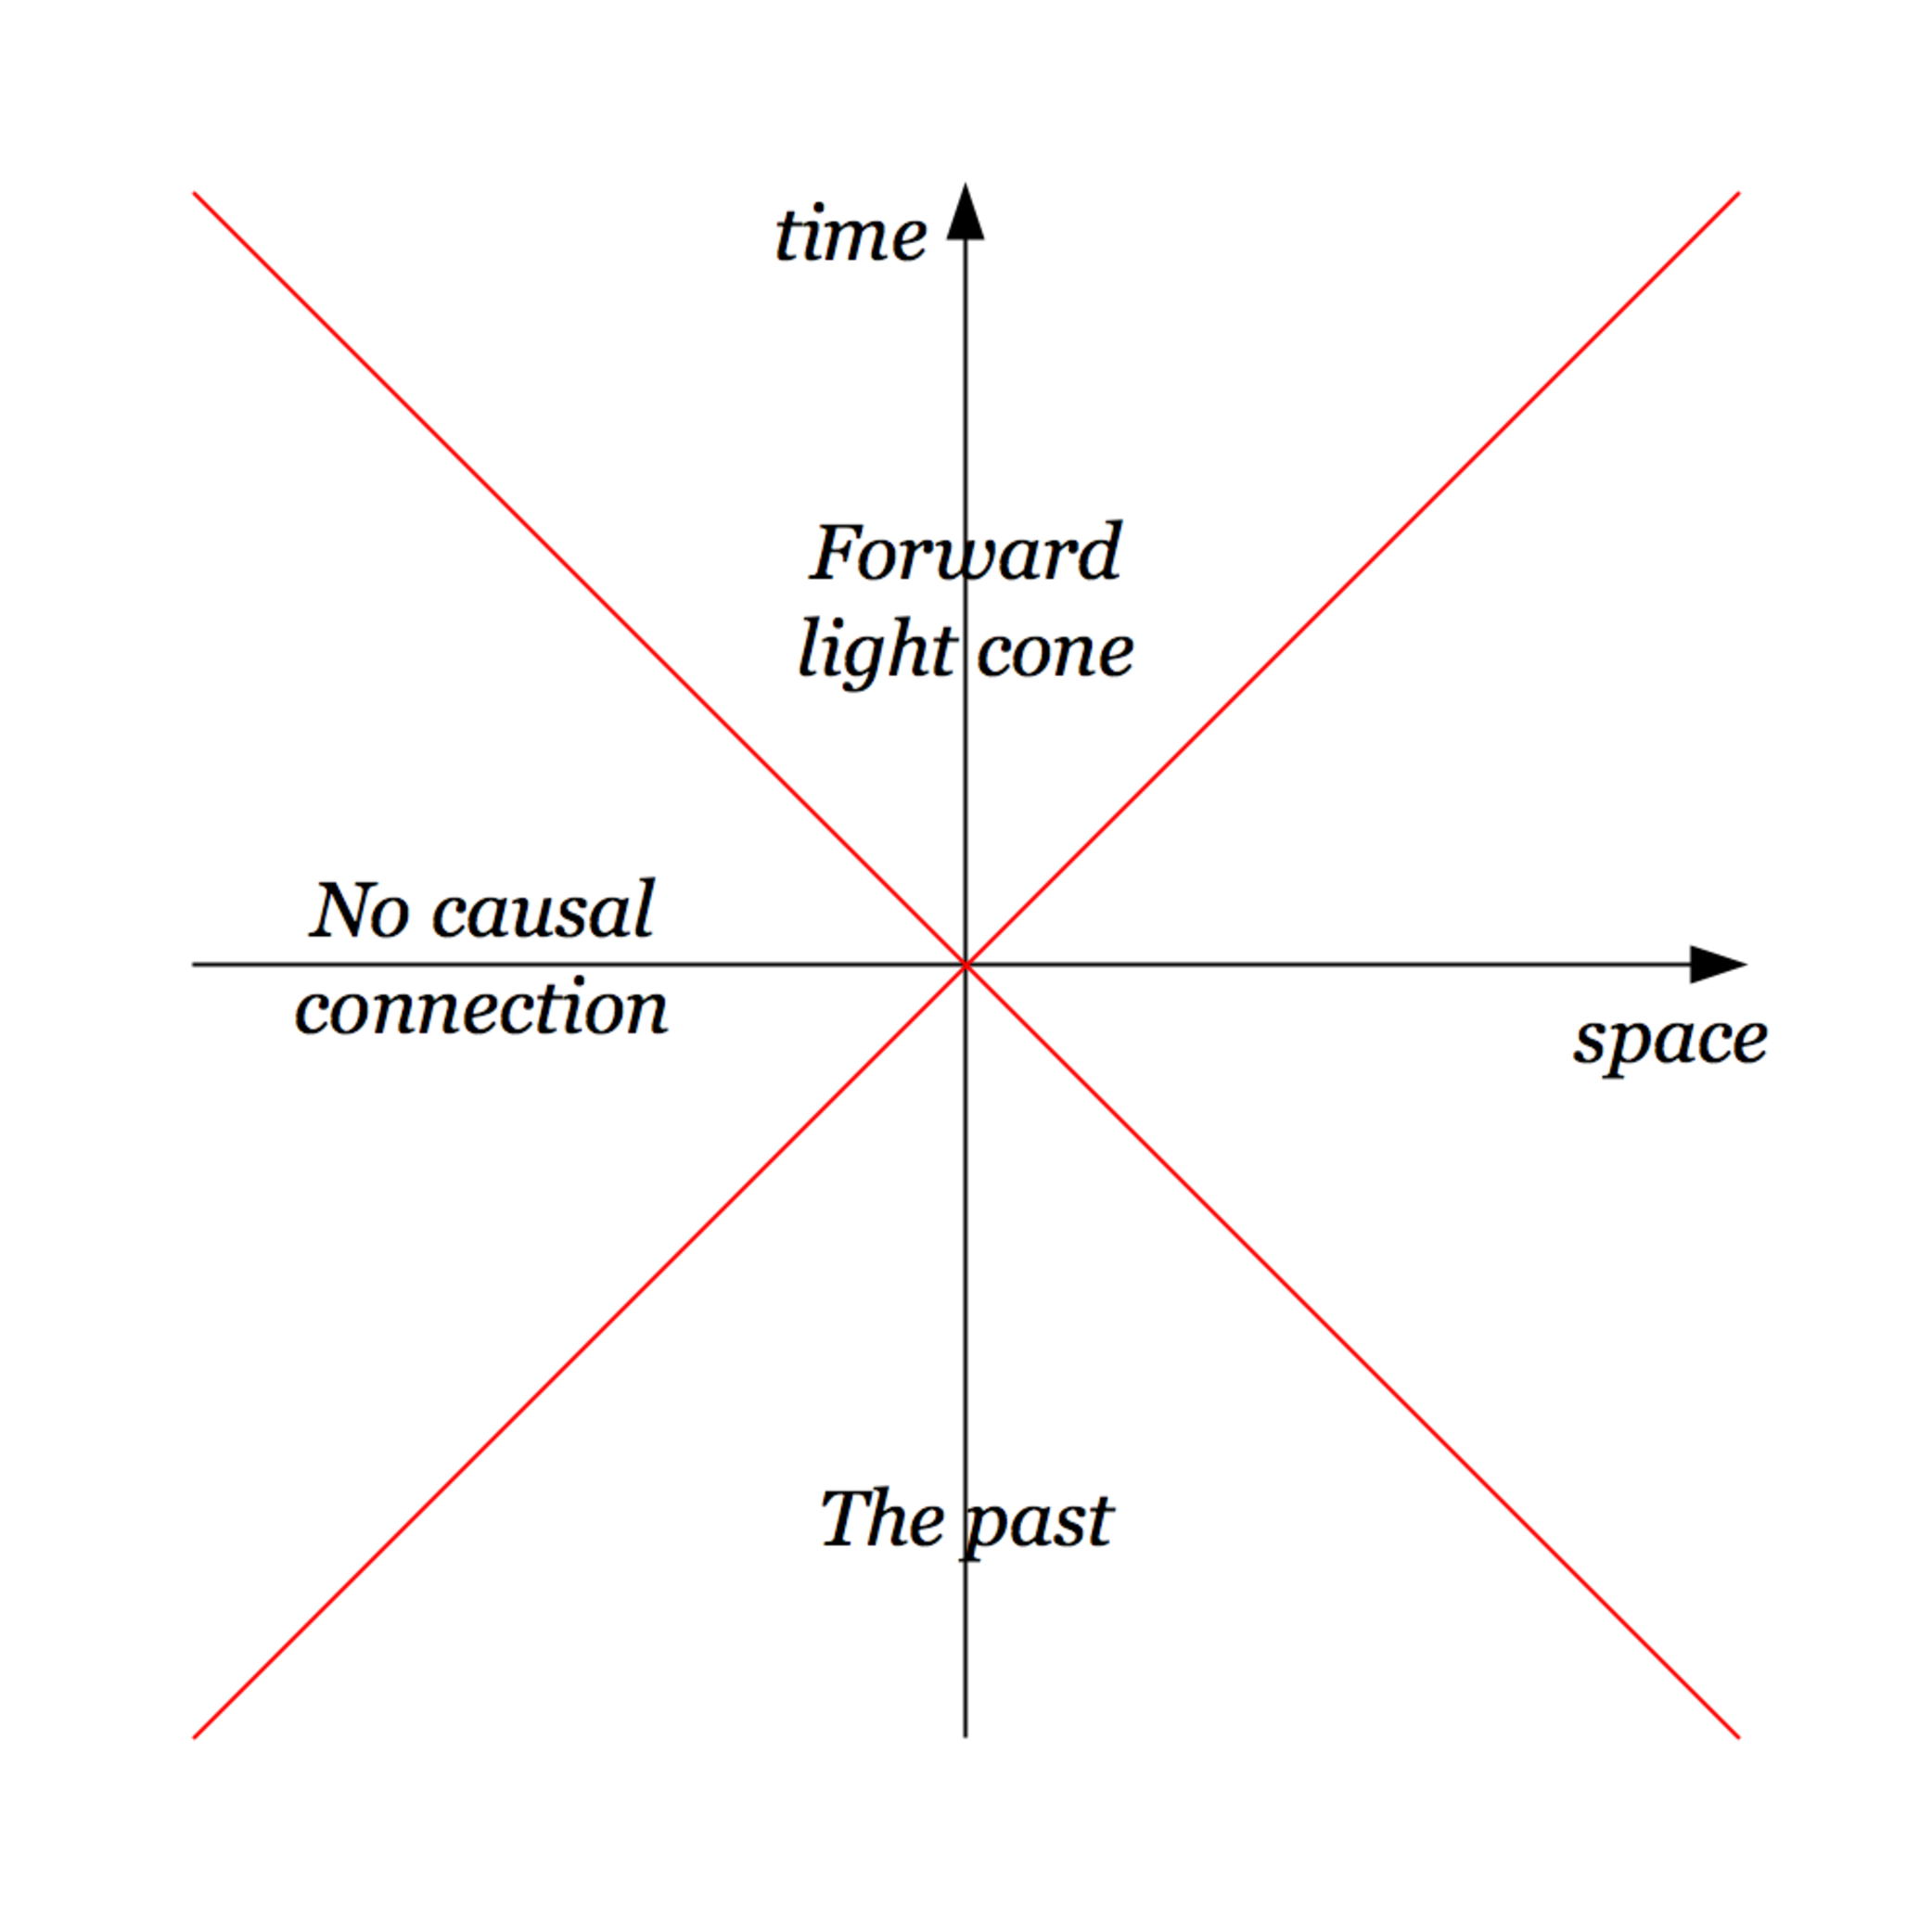
\includegraphics[width=0.75\textwidth]{images/chapter_5/lightcone.pdf}
    \caption[The light cone]{The light cone, showing distinct regions of spacetime which are and are not causally connected.  The red lines show the boundaries of these regions.}
    \label{fig:ch5_lightcone}
  \end{center}
\end{figure}

\section{Relativistic kinematics}

Usually, one of two processes is considered, either $A \to B + C$ (decay) or $A + B \to C + D$ (scattering).  For a decay the centre of mass energy is the mass of the particle $A$.  For scattering:

\[
  s = (p^{\mu}_A + p^{\mu}_B)^2 = (p^{\mu}_c + p^{\mu}_D)^2
\]

For a fixed target experiment $B$ is at rest:

\begin{eqnarray*}
  s & = & (E_A + E_B)^2 - (\ul{p}_A + \ul{p}_B)^2 \\
    & = & (E_A + m_B)^2 - P^2_A \\
    & = & m^2_A + m^2_B + 2m_BE_A \\
    \textrm{If } E_A & \gg & m_A, m_B \textrm{ then:} \\
    \sqrt{s} & \simeq & \sqrt{2E_A m_B}
\end{eqnarray*}

\subsection{Centre of mass frame}

\begin{eqnarray*}
  s & = & \left(p^{\mu}_A + p^{\mu}_B \right)^2 \\
    & = & \left(E^{CMS}_A + E^{CMS}_B\right)^2 - \left(p^{CMS}_A + p^{CMS}_B\right)^2 \\
    & = & \left(E^{CMS}_A\right)^2 + 2E^{CMS}_AE^{CMS}_B + \left(E^{CMS}_B\right)^2 \\
  \textrm{So } \sqrt{s} & = & E^{CMS}_A + E^{CMS}_B
\end{eqnarray*}

At Tevatron $E_P = E_{\bar{p}} = 980 GeV$, so $\sqrt{s} \simeq 2TeV$.

At HERA $E_p = 920GeV$, $E_e = 27.5GeV$, so $\sqrt{s} = 318GeV$.

To transform between the centre of mass frame and the laboratory frame it is necessary to determine $\beta$ and $\gamma$:

\begin{eqnarray*}
  \beta & = & \frac{\textrm{Three momentum part of four vector}}{\textrm{Energy part of four momentum}} \\
  & = & \frac{|\ul{p}_A| + |\ul{p}_B|}{E_A + E_B} \\
  \gamma & = & \frac{\textrm{Energy part of four momentum}}{\textrm{Centre of mass energy}} \\
  & = & \frac{|\ul{p}_A| + |\ul{p}_B|}{\sqrt{s}}
\end{eqnarray*}

The energy and momentum of a particle in the centre of mass frame can be determined using invariance rather than Lorentz transformations:

\begin{eqnarray*}
  p^{\mu}_A + p^{\mu}_B & = & \left(\sqrt{s},0\right) \textrm{ in the centre of mass frame} \\
  p_{A\mu}\left(p^{\mu}_A + p^{\mu}_B \right) & = & \left(E^{CMS}_A,\ul{p}^{CMS}_A\right) \cdot \left(\sqrt{s},0\right) \\
  \Rightarrow p_{A\mu} \left(p^{\mu}_A + p^{\mu}_B\right) & = & E^{CMS}_A \sqrt{s} \\
  m^2_a + p_{A\mu}p^{\mu}_B & = & E^{CMS}_A \sqrt{s} \\
  \textrm{Recall } s & = & \left( p^{\mu}_A + p^{\mu}_B\right)\left(p_{A\mu} + p_{B\mu}\right) \\
  & = & p_A \cdot p_A + p_B \cdot p_B + 2p^{\mu}_A\cdot p_{B\mu} \\
  \textrm{So } p_{A\mu}p^{\mu}_B & = & \frac{s - m^2_A - m^2_B}{2} \\
  \textrm{So } E^{CMS}_A & = & \frac{2m^2_A + s - m^2_A - m^2_B}{2\sqrt{s}} \\
  \Rightarrow E^{CMS}_A & = & \frac{s + m^2_A - m^2_B}{2\sqrt{s}}
\end{eqnarray*}

And similarly for the other energies.

\begin{eqnarray*}
  \left( p^{CMS}_A \right)^2 & = & \left( E^{CMS}_A \right)^2 - m^2_A \\
  \textrm{So } \left(p^{CMS}_A\right)^2 & = & \left( \frac{s + m^2_A - m^2_B}{2\sqrt{s}}\right)^2 - m^2_A \\
  & = & \frac{\left(s + m^2_A - m^2_B\right)^2}{4s}-m^2_A \\
  & = & \frac{s^2 + \left(m^2_A - m^2_B\right)^2 + 2sm^2_A - 2sm^2_B - 4sm^2_A}{4s} \\
  & = & \frac{s^2 + \left(m^2_A - m^2_B\right)^2 - 2s\left(m^2_A + m^2_B\right)}{4s} \\
  & = & \frac{\lbrack s - \left(m_A + m_B\right)^2\rbrack \lbrack s - \left(m_A - m_B\right)^2 \rbrack}{4s}
\end{eqnarray*}

\subsection{Mandelstan variables}

The Mandelstan variables are shown in figure \ref{fig:ch5_mandelstan}.

\begin{figure}[!htb]
  \begin{center}
    \begin{tabular}{ccc}
      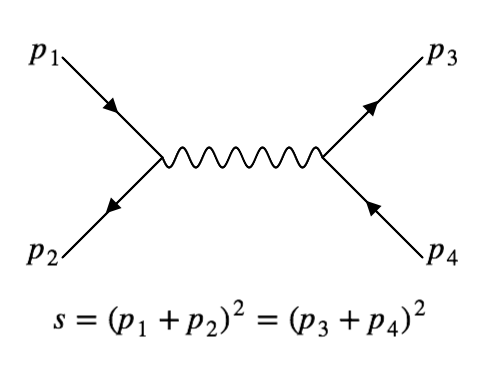
\includegraphics[width=0.4\textwidth]{images/web_feynman/image_17.png}
      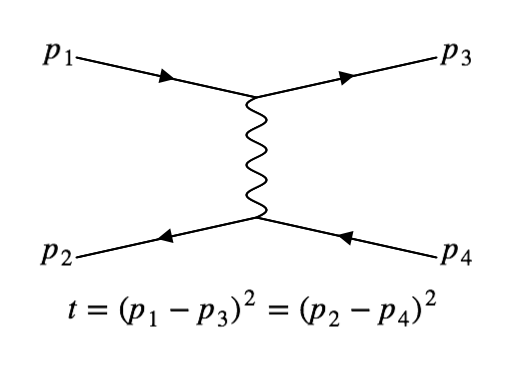
\includegraphics[width=0.4\textwidth]{images/web_feynman/image_18.png}
      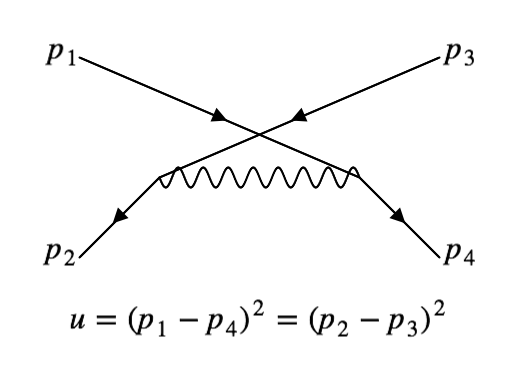
\includegraphics[width=0.4\textwidth]{images/web_feynman/image_19.png}
    \end{tabular}
    \caption[Mandelstan variables]{The Mandelstan variables are relativistically invariant kinematic quantities.}
    \label{fig:ch5_mandelstan}
  \end{center}
\end{figure}

\begin{eqnarray*}
  s & = & \left(p_A + p_B\right)^2 \\
  t & = & \left(p_A - p_C\right)^2 \\
    & = & \left(p_B - p_D\right)^2 \\
    & = & -Q^2 = q^2 \\
  u & = & \left(p_A - p_D\right)^2 \\
    & = & \left(p_C - p_B\right)^2 \\
    s + t + u & = & m^2_A + m^2_B + m^2_C + m^2_D \\
    \textrm{Proof: } s + t + u & = & \left(p_A + p_B\right)^2 + \left(p_A - p_C\right)^2 + \left(p_A - p_D\right)^2 \\
    & = & p^2_A + P^2_B + 2p_Bp_A + p^2_A + p^2_C - 2p_Ap_C + p^2_A + p^2_D - 2p_Ap_D \\
    & = & 3m^2_A + m^2_B + m^2_C + m^2_D + 2\left(p_Bp_A - p_Ap_C - p_Ap_B\right) \\
    & = & 3m^2_A + m^2_B + m^2_C + m^2_D + 2p_A\left(p_B - p_C - p_D\right) \\
    \textrm{But } p_A + p_B & = & p_C + p_D \\
    \Rightarrow p_B - p_C - p_D & = & -p_A \\
    \textrm{So } s + t + u & = & m^2_A + m^2_B + m^2_C + m^2_D
\end{eqnarray*}

\section{Relativistic spin\texorpdfstring{$-0$}{-0} particles}

\subsection{The Klein-Gordon equation}

The quantum wavefunction for a free scalar particle propagating in the $x-$direction is:

\begin{eqnarray*}
  \phi & \sim & \e^{i(px - Et)} \\
       & \sim & \e^{ip^{\mu}x_{\mu}}
\end{eqnarray*}

Repeating the procedure that yielded the Schroedinger equation, but using:

\begin{equation}
  E^2 = p^2 + m^2 \textrm{ (rather than }E = p^2/2m\textrm{)} \label{eq:relativisticmass}
\end{equation}

\begin{equation}
  \begin{array}{ccc}
  E & \to & i\frac{\partial}{\partial t} \\
  \ul{p} & \to & -i\ul{\nabla}
  \end{array}
  \Bigg\}
  \label{eq:relativisticep}
\end{equation}

Combining (\ref{eq:relativisticmass}) and (\ref{eq:relativisticep}) and transforming in an equation acting on $\phi$ gives:

\begin{eqnarray}
  \frac{\partial^2\phi}{\partial t^2} & = & -\nabla^2\phi + m^2\phi
  \label{eq:kleingordon} \\
  \textrm{Or } \Box^2\phi & = & m^2 \phi \nonumber
\end{eqnarray}

(\ref{eq:kleingordon}) is the Klein-Gordon equation (or the relativistic Schroedinger equation.  The complex conjugate of (\ref{eq:kleingordon}) is:

\begin{eqnarray}
  -\frac{\partial^2\phi^{\star}}{\partial t^2} = & -\nabla^2\phi^{\star} + m^2\phi^{\star} &\label{eq:kleingordonconjugate} \\
  \phi^{\star}\times(\ref{eq:kleingordon}) = & -\phi^{\star}\frac{\partial^2\phi}{\partial t^2} & = -\phi^{\star}\nabla^2\phi + m^2\phi^{\star}\phi \label{eq:phistarphi} \\
  \phi\times(\ref{eq:kleingordonconjugate}) = & -\phi\frac{\partial^2 \phi^{\star}}{\partial t^2} & = -\phi\nabla^2\phi^{\star} + m^2\phi\phi^{\star} \label{eq:phiphistar} \\
  -i\left( (\ref{eq:phistarphi}) - (\ref{eq:phiphistar}) \right) = & i\left( \phi^{\star}\frac{\partial^2\phi}{\partial t^2}- \phi\frac{\partial^2\phi}{\partial t^2}\right) & = i\left(\phi^{\star}\nabla^2\phi - \phi\nabla^2\phi^{\star} \right) \nonumber
\end{eqnarray}
\begin{eqnarray}
  \Rightarrow i \frac{\partial}{\partial t}\Bigg[ \phi^{\star}\frac{\partial \phi}{\partial t} - \phi\frac{\partial \phi^{\star}}{\partial t}\Bigg] - i\ul{\nabla}\lbrack \phi^{\star}\ul{\nabla}\phi - \phi\ul{\nabla}\phi_{\star}\rbrack & = 0 & \nonumber \\
  \textrm{or } \frac{\partial \rho}{\partial t} + \ul{\nabla}\cdot\ul{j} & = 0 & \nonumber
\end{eqnarray}

\begin{eqnarray*}
  \rho & = & i\left(\phi^{\star}\frac{\partial\phi}{\partial t} - \phi\frac{\partial \phi^{\star}}{\partial t} \right) \\
  \ul{J} & = & i\left( \phi^{\star}\ul{\nabla}\phi - \phi\ul{\nabla}\phi^{\star}\right) 
\end{eqnarray*}

Consider the form of $\rho$ for $\phi = N\e^{i\ul{p}\cdot{\ul{x}}}$:

\begin{eqnarray*}
  \phi & = & N\e^{i\left(px - Et\right)} \\
  \rho & = & i\left(\phi^{\star}\frac{\partial \phi}{\partial t} - \phi \frac{\partial \phi^{\star}}{\partial t}\right) \\
  & = & i \left( N^{\star}\e^{-i\left(px-Et\right)}\left(-iE\right)N\e^{i\left(px-Et\right)} - N\e^{i\left(px-Et\right)}\left(iE\right)N^{\star}\e^{-1\left(px-Et\right)}\right) \\
  & = & i\lbrack N^{\star}N\left(-iE\right) - NN^{\star}\left(ie\right) \rbrack \\
  & = & 2N^{\star}NE \\
  \textrm{So } \rho & = & 2EN^{\star}N
\end{eqnarray*}

Similarly $\ul{j} = 2N^{\star}N\ul{p}$.

This appeared disastrous because $E^2 = p^2 + m^2$ lead to negative energy solutions (ie $E_- = -\sqrt{p^2 + m^2}$) which lead to negative probability densities, $\rho<0$.  Note that $\rho$, being proportional to $E$ may have been antiticipated.  Under a Lorentz boost of speed $v$ the volume element undergoes a contraction:

\[
  \mathrm{d}^3r \to \gamma\mathrm{d}^3r
\]

Therefore to keep $\rho \mathrm{d}^3r$ invariant $\rho$ must transform as a time-like component:
\[
  \rho \to \gamma \rho
\]

\subsection{The perceived distaster of the Klein-Gordon equation}

The problem faced is that the Klein-Gordon equation can give $\rho<0$.  There are two steps to remove this problem which works for scalar particles.  In 1934 Pauli and Weisskopf derived the Klein-Gordon equation by multiplying $\ul{j} = \left(\rho, \ul{j}\right)$ by the charge of the particle, so $q\ul{j}^{\mu}$ becomes $\ul{j}^{\mu}_{em}$:

\[
  \ul{j}^{\mu}_{em} = -i\e\left(\phi^{\star}\partial^{\mu}\phi - \phi\partial^{\mu}\phi^{\star} \right)
\]

where $-\e$ is the charge on the scalar electron.  Now $\rho = j^0_{em}$ is a charge densiity and not a probability density, so $\rho$ can be negative.

\subsection{The Feynmann-Stueckelberg interpretation of \texorpdfstring{$E<0$}{ELO0} solutions}

The approach taken by Feynmann and Stueckelberg is that the negative energy solutions describe a negative energy particle propagating backwards in time or equivalently, a positive energy antiparticle propagating forwards in time.  Consider an electron of energy $E$, momentum $\ul{p}$ and charge $-\e$:

\[
  \ul{j}_{em}(\e^-) = -2eN^{\star}N(E,\ul{p})
\]

For a positron the charge is $\e$:

\[
  \ul{j}_{em}(\e^+) = 2\e N^{\star}N(E,\ul{p})
\]

which is equivalent to:

\[
  \ul{j}_{em}(\e^-) = -2\e N^{\star}N(-E,-\ul{p})
\]

which is the same as $\ul{j}_{em}$ but with $(-E,-\ul{p})$ so the emission of a positron of energy $E$ is the same as the absorption of an electron with energy $-E$.  These ideas can describe many particle interactions.  Consider a double scattering process in an interaction region, as shown in figure \ref{fig:ch5_paths}.

\begin{figure}[!htb]
  \begin{center}
    \begin{tabular}{cc}
      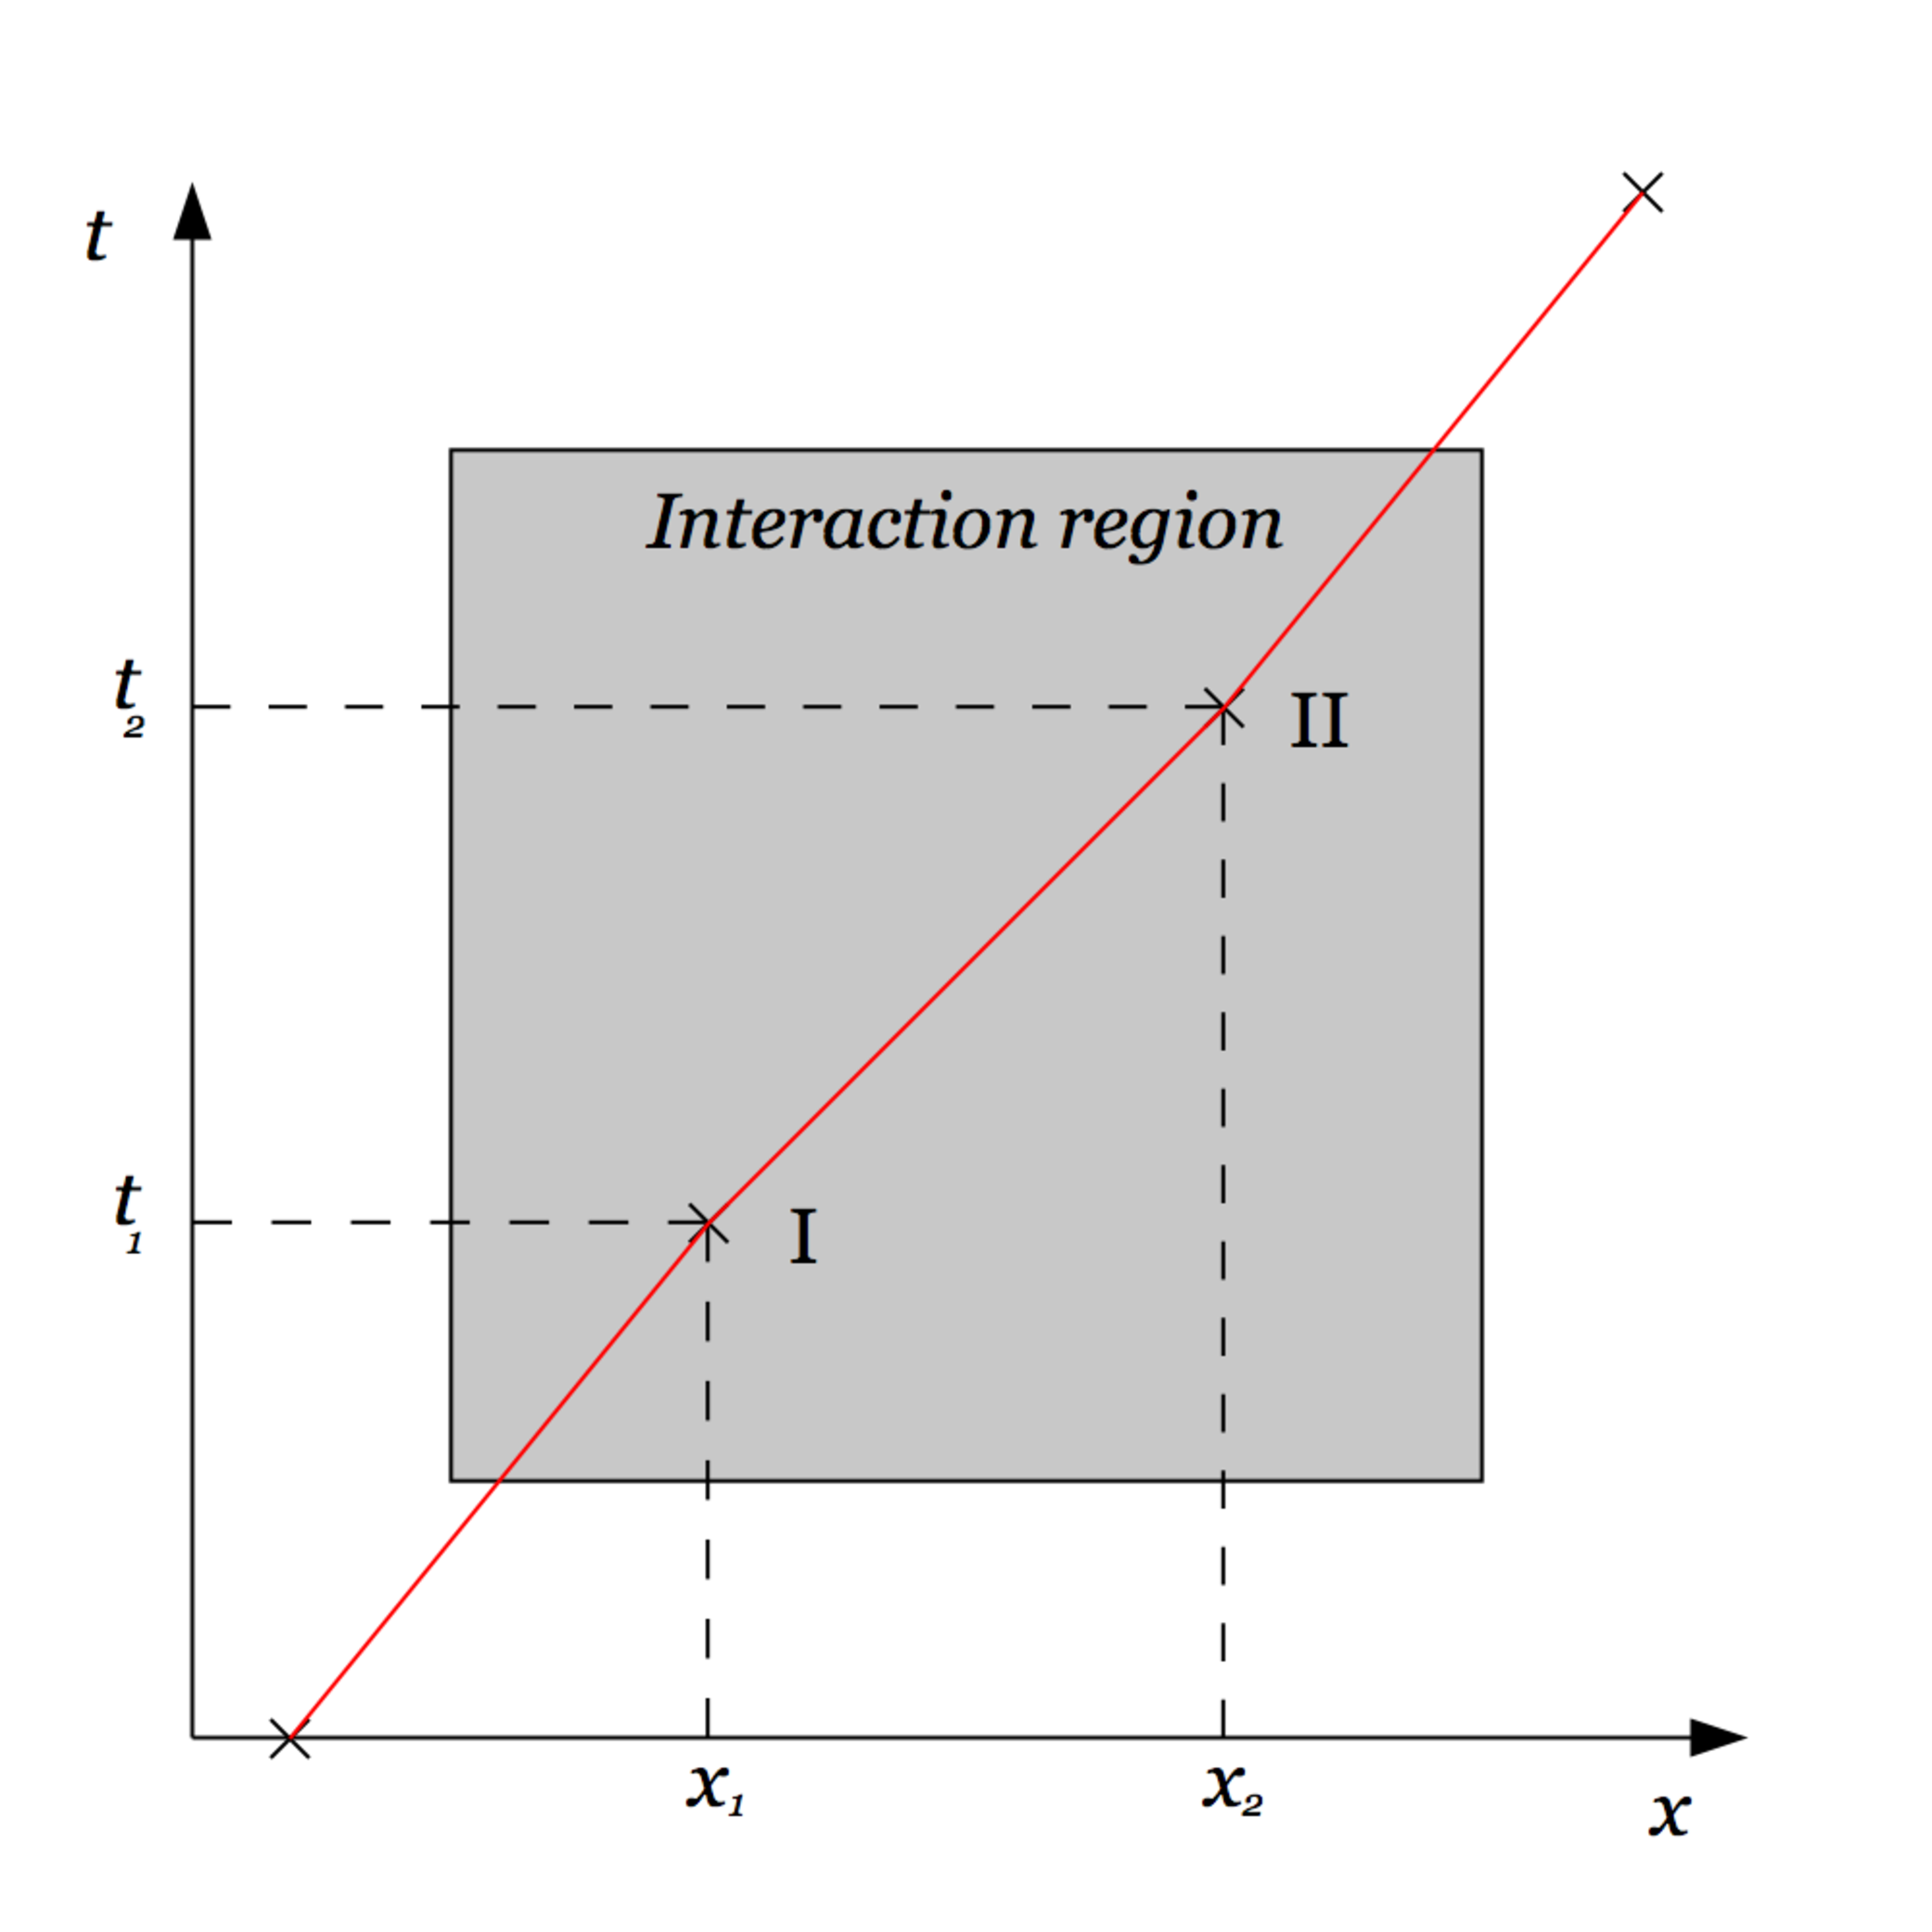
\includegraphics[width=0.5\textwidth]{images/chapter_5/path1.pdf} &
      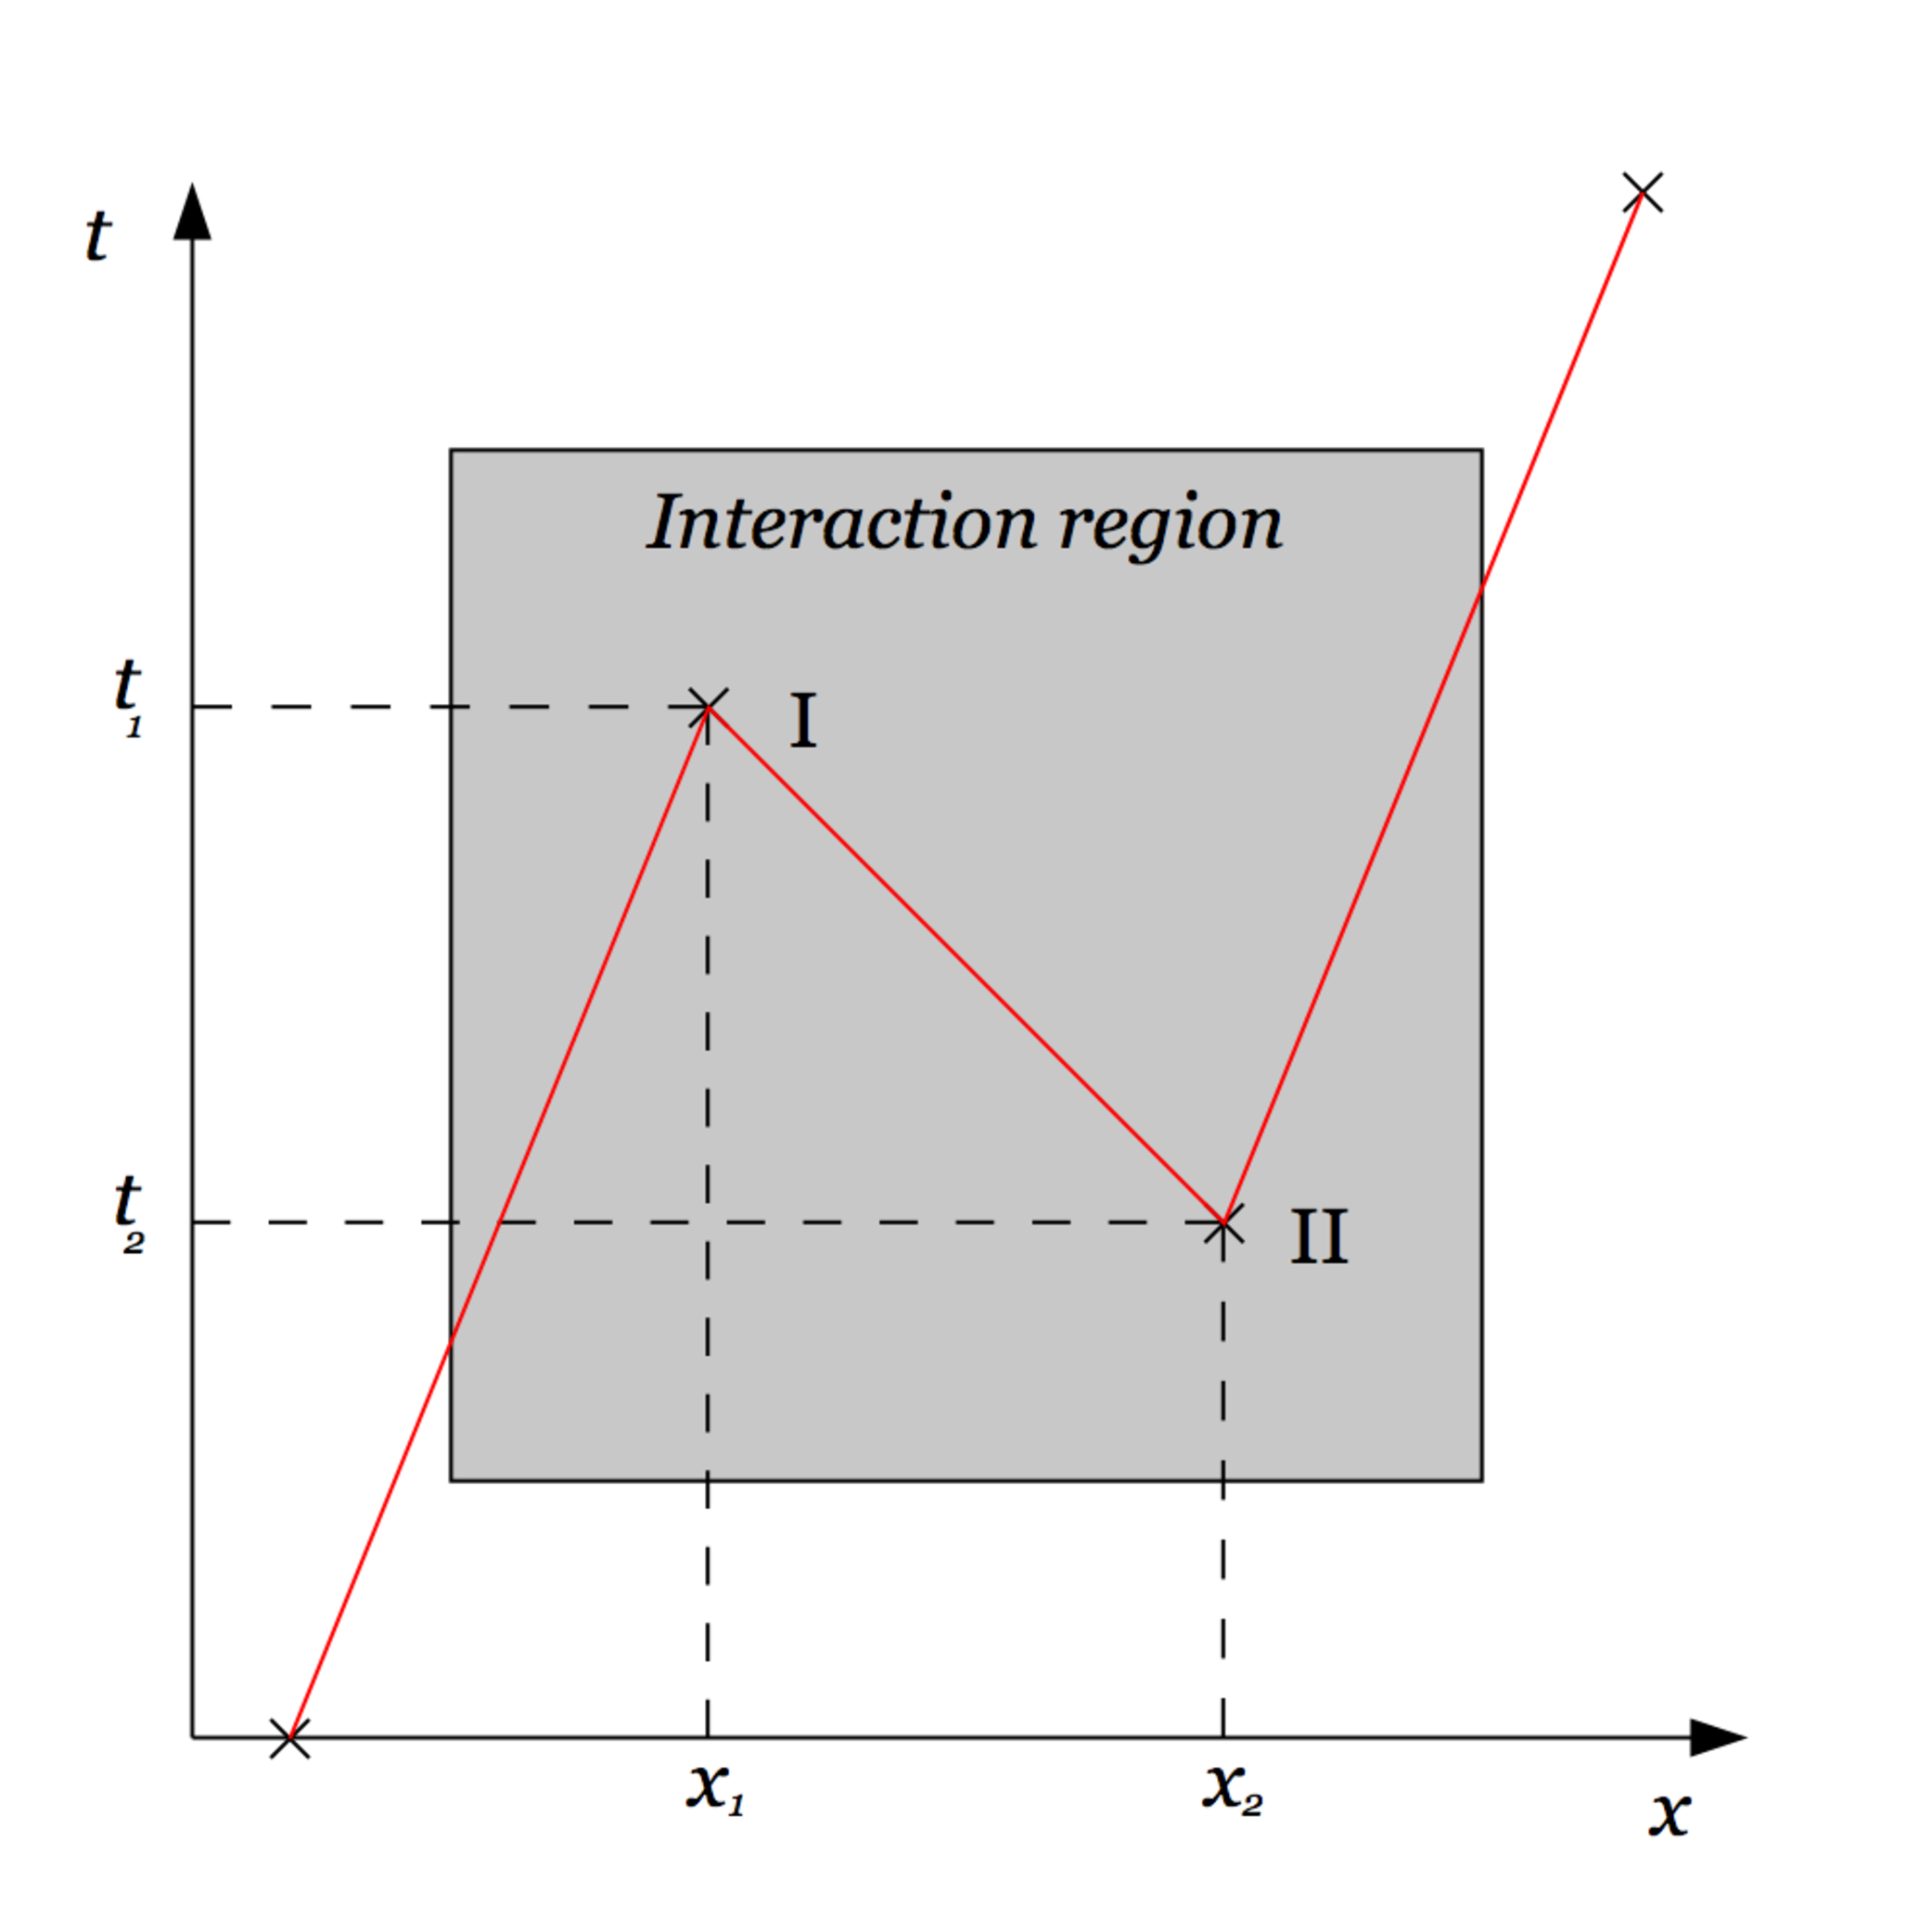
\includegraphics[width=0.5\textwidth]{images/chapter_5/path2.pdf} \\
    \end{tabular}
    \caption[A causal and a non-causal path of a particle]{Two paths of a particle, one of which respects causality (left), and one of which violates causality (right).}
    \label{fig:ch5_paths}
  \end{center}
\end{figure}

For the first diagram, at time $t_1$ and position $\ul{r}_1$ the electron scatters at $I$ and then at a later time $t_2$ and position $\ul{r}_2$ scatters at $II$.  All particles go forwards in time.  For the second diagram, at the earlier time $t_1$ and position $\ul{r}_1$ an electron-positron pair is created at $I$.  The electron leaves the volume and the positron propagates forwards in time to $t_2$ and $\ul{r}_1$ where it annihilates with an electron at $II$.

Both of the above diagrams have the same initial and final state, but the first involves just one electron while the second involves three particles.  They would both have to be included when calculating the probability of that process occuring.

\cleardoublepage
% Copyright Aidan Randle-Conde 2007-2014
% http://www.aidansean.com/phd_notes
% Anyone is free to download, redistribute, edit and use these notes and the source tex files with the following restrictions:
% This 
%  This message is included in the tex source files.
%  Aidan Randle-Conde is credited as the author.
%  Images are correctly credited to their respective authors, as outlined in the references.
%  No part of these notes may be used for commercial purposes.

\chapter{Calculating amplitudes}

\section{Possible approaches}

\begin{itemize}
  \item Make the Born approximation relativistic, which is the Feynmann-Stueckelberg approach.  This is not so easy to make systematic and is rather ad hoc.  This method motivates the propagator.
  \item Make non-relativistic perturbation theory relativistic, as in Halzen and Martin.  This is not systematic and does not motivate the propagator.
  \item Canonical field theory enables a more systematic approach, but it takes more time.
  \item The path integral approach is systematic but mathematically more challenging.
\end{itemize}

\section{Propagator approach}

The basic idea behind the propagator approach is to know the quantum wave (which is called $\psi(\ul{r}',t')$) given the wavefunction at initial coordinates $\psi(\ul{r},t)$.

\[
  \psi(\ul{r}',t') = i\int G(\ul{r}',t,\ul{r},t)\psi(\ul{r},t)\mathrm{d}^3r \textrm{ for } t' > t
\]

where $G$ is a Green's function.

The wave at $\ul{r}$ has been propagated by $G$ to $\ul{r}'$.  Consdier the scattering process.  An incident particle described by the plane quantum wave $\phi(\ul{r},t)$ is incident on a potential $V(\ul{r},t)$.  Schroedinger's equation should describe what happens.  Recall:

\begin{eqnarray*}
  \left(H_0 + V\right)\psi & = & i\frac{\partial \psi}{\partial t} \\
  i\partial\psi(\ul{r},t) - H_0\psi(\ul{r},t)\mathrm{d}t & = & V(\ul{r},t)\psi(\ul{r},t)\mathrm{d}t
\end{eqnarray*}

Suppose the potential acts at $\ul{r}_1$ and $t_1$ for a short time interval $\Delta t_1$:

\begin{eqnarray*}
  \Rightarrow i\int\partial\psi(\ul{r}_1,t_1) - \int_{t_1}^{t_1+\Delta t_1}H_0\psi(\ul{r},t_1)\mathrm{d}t_1 & = & \int_{t_1}^{t_1+\Delta t_1} V(\ul{r}_1,t_1)\psi(\ul{r}_1,t_1)\mathrm{d}t_1 \\
  \Delta\psi(\ul{r}_1,t_1) & = & -iV(\ul{r}_1,t_1)\psi(\ul{r}_1,t_1)\Delta t_1
\end{eqnarray*}

where $H_0$ does not contribute significantly.

\begin{eqnarray*}
  \Delta \psi(\ul{r}_1,t_1) & \sim & -iV(\ul{r}_1,t_1)\phi(\ul{r}_1,t_1)\Delta t_1 \\
  \textrm{where } \psi(\ul{r}_1,t_1) & = & \phi(\ul{r}_1,t_1) + \Delta \psi(\ul{r}_1,t_1) \\
  \Delta\psi(\ul{r}',t') & = & i \int \mathrm{d}^3r_1 G_0(\ul{r}',t';\ul{r}_1,t_1)\Delta\psi(\ul{r}_1,t_1) \\
  & = & i\int\mathrm{d}^3r_1 G_0(\ul{r}',t';\ul{r}_1,t_1)(-i)V(\ul{r}_1,t_1)\phi(\ul{r}_1,t_1)\Delta t_1 \\
  \textrm{ie } \psi(\ul{r}',t') & = & \phi(\ul{r}',t') + \int\mathrm{d}^3r_1 G_0(\ul{r}',t';\ul{r}_1,t_1)V(\ul{r}_1,t_1)\phi(\ul{r}_1,t_1)\Delta t_1 \\
  \psi(\ul{r}',t') & = & \phi(\ul{r}',t') + \int \mathrm{d}^4x_1 G_0(x';1)V(1)\phi(1) \\
  \textrm{where }V(1) & = & V(\ul{r}_1,t_1) \textrm{ etc and } x' \textrm{ is now a 4 vector.}
\end{eqnarray*}

Now applying a potential at $(\ul{r}_2,t_2)$ for $\Delta t_2$ generates the wavefunction:

\begin{eqnarray*}
  \psi(\ul{r}',t') & = & \phi(\ul{r}',t) + \int \mathrm{d}^3r_1G_0(x';1)V(1)\phi(1)\Delta t_1 \\
                          &   & + \int \mathrm{d}^3r_2 G_0(x';2)V(2)\phi(2)\Delta t_2 \\
                          &   & + \int\int \mathrm{d}^3r_1 \mathrm{d}^3r_2 G_0(x';2)V(2)G_0(2;1)V(1)\phi(1)\Delta t_1 \Delta t_2
\end{eqnarray*}

Integrating over $\Delta t_1$, $\Delta t_2$ gives:

\[
  \psi(\ul{r}',t') = \phi(\ul{r}',t') + \int\mathrm{d}^4x_1 G_0(x';1)V(1)\phi(1) + \int\int\mathrm{d}^4x_1 \mathrm{d}^4x_2 G_0(x';2)V(2)G_0(2;1)V(1)\phi(1)
\]

Now it is necessary to evaluate $G_0$.  In particular $G_0(2;1)$ ie the $G_0$ for the intermediate states:

\[
  \psi(\ul{r}',t') = i\int_{t'>t} \mathrm{d}^3r G(x';x)\psi(\ul{r},t)
\]

This can be written in a form valid for all times (using the Heaviside step function centred at $\tau = t'$):

\begin{eqnarray*}
  \theta(t'-t)\psi(x') & = & i\int \mathrm{d}^3r G(x';x)\psi(x) \\
  \theta(t'-t) = \Bigg\{
    \begin{array}{cc}
    1 & t'>t \\
    0 & \textrm{otherwise}
    \end{array}
\end{eqnarray*}

Applying the Schroedinger equation to both sides:

\begin{eqnarray*}
  LHS & : & \Bigg[ i\frac{\partial}{\partial t} - H(x')\Bigg] \theta(t'-t)\psi(x') \\
  & = & i\delta(t'-t)\psi(x') + \theta(t'-t)i\frac{\delta}{\delta t}\psi(x') -H(x')\theta(t'-t)\psi(x') \\
  & = & i\delta(t'-t)\psi(x') \\
  RHS & : & i\int\mathrm{d}^3r\Bigg[ i\frac{\partial}{\partial t'} - H(x')\Bigg] G(x';x)\psi(x)
\end{eqnarray*}

Consider a particle in the absence of a potential ie $V = 0$, then solve explicitly for the free particle propagator.

\[
  RHS : i\int\mathrm{d}^3r\Bigg[ E - \frac{p^2}{2m}\Bigg] G_0(x';x)\psi(x)
\]

Transforming to four-momentum space via a Fourier transform:

\begin{eqnarray*}
  RHS & : & i\int\frac{\mathrm{d}^3p}{(2 \pi)^3}\frac{\mathrm{d}E}{2\pi}\left(E - \frac{p^2}{2m}\right)G_0(E;\ul{p}) \e^{i\ul{p}(\ul{r'}-\ul{x})}\e^{-iE(t'-t)}\psi(x) \\
  LHS & : & i\delta(t'-t)\psi(x') \\
      & = & i\delta(t'-t)\int\mathrm{d}^3r\psi(x)\delta^3(\ul{r}' - \ul{r}) \\
      & = & i\delta^4(x'-x)\psi(x) \\
  LHS & = & RHS \textrm{ so:} \\
  i\delta^4(x'-x)\psi(x) & = & i\int\frac{\mathrm{d}^3p}{(2\pi)^3}\frac{\mathrm{d}E}{2\pi}\left(E - \frac{p^2}{2m}\right)G_0(E;p)\e^{ip(x'-x)}\e^{-E(t'-t)}\psi(x) \\
  \Rightarrow \delta^4(x'-x)\psi(x) & = & \int\frac{\mathrm{d}^4p}{(2\pi)^4}\e^{ip(x'-x)}\e^{-iE(t'-t)}\psi(x) \\
  \textrm{where } G_0 & = & \frac{1}{E - \frac{p^2}{2m}} \textrm{ for } E \neq \frac{p^2}{2m}
\end{eqnarray*}

As $E = p^2/2m$ the value of $G_0$ becomes undefined.  The simple model cannot account for the singularity, so a new term in introduced:

\[
  G_0 \to G_0 = \frac{1}{E - \frac{p^2}{2m} + i\epsilon}
\]

The free particle propagator for  real or virtual particle in momentum space is the inverse of the free particle Schroedinger equation.  Assume that in momentum space the free propagators of the Klein-Gordon equation, Dirac equation and Proca equation are all obtained by inverting the appropriate equation.

\cleardoublepage
% Copyright Aidan Randle-Conde 2007-2014
% http://www.aidansean.com/phd_notes
% Anyone is free to download, redistribute, edit and use these notes and the source tex files with the following restrictions:
% This 
%  This message is included in the tex source files.
%  Aidan Randle-Conde is credited as the author.
%  Images are correctly credited to their respective authors, as outlined in the references.
%  No part of these notes may be used for commercial purposes.

\chapter{Spinless \texorpdfstring{$\lowercase{e}^- \mu^-$}{EMu} scattering}

\section{Electrodynamics of spinless particles}

\begin{figure}[!htb]
  \begin{center}
    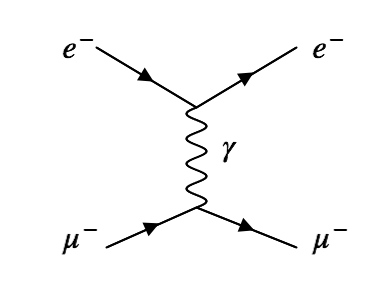
\includegraphics[width=0.5\textwidth]{images/web_feynman/image_20.png}
    \caption[Spinless $e-\mu$ scattering]{Feynman diagram showing spinless $e-\mu$ scattering.}
    \label{fig:ch7_EMuToEMu}
  \end{center}
\end{figure}

Consider spinless electrons scattering off spinless muons, as shown in figure \ref{fig:ch7_EMuToEMu}.  Starting with the Klein-Gordon equation and including the electromagnetic interaction will lead to a simple model of scattering.  In electrodynamics the motion of a particle of charge $-\e$ in an electromagnetic potential $A^{\mu} (= (A^0,\ul{A}))$ is obtained by the substitution:

\begin{eqnarray*}
  p^{\mu} & \to & p^{\mu} + \e A^{\mu} \\
  \textrm{So } p_{\mu}p^{\mu} = m^2 & \to & \left(p_{\mu} + \e A_{\mu} \right)\left(p^{\mu} + \e A^{\mu}\right) = m^2
\end{eqnarray*}

In quantum mechanics this is:

\begin{eqnarray*}
  \left(i\partial_{\mu} + \e A_{\mu}\right)\left(i\partial^{\mu} + \e A^{\mu}\right)\phi & = & m^2 \phi \\
  -\partial_{\mu}\partial^{\mu}\phi + i\e \partial_{\mu}A^{\mu}\phi + i\e A_{\mu}\partial^{\mu}\phi + \e^2A_{\mu}A^{\mu}\phi & = & m^2\phi \\
  \Rightarrow \partial_{\mu}\partial^{\mu} + m^2\partial & = & ie\partial_{\mu}A^{\mu}\phi + i\e A_{\mu}\partial^{\mu}\phi + \e^2A_{\mu}A^{\mu}\phi \\
  & = & -V\phi
\end{eqnarray*}

where $V$ is the electromagnetic perturbation and the minus sign is required to that there is the same relateive sign to the $p^2/2m$ term in the Schroedinger equation.

The transition amplitude is:

\begin{eqnarray*}
  T_{fi} & = & -i\int\mathrm{d}^4x\phi^{\star}_f(x)V(x)\phi_i(x) \\
         & = & -i\int\mathrm{d}^4x\phi^{\star}_f(x)(-i\e)(\partial_{\mu}A^{\mu} + A_{\mu}\partial^{\mu})\phi_2(x)
\end{eqnarray*}
where the second order term is neglected.

Transforming the first term so that the derivative acts on $\phi^{\star}_f$:

\begin{eqnarray*}
  T_{fi} & = & \int \phi^{\star}_f \partial_{\mu}\left(A^{\mu}\phi_2\right)\mathrm{d}^4x + \cdots \\
  I & = & \int \phi^{\star}_f\partial_{\mu}\left(A^{\mu}\phi_2\right)\mathrm{d}^4x \\
  \int u\frac{\mathrm{d}v}{\mathrm{d}x}\mathrm{d}x & = & uv - \int v \frac{\mathrm{d}u}{\mathrm{d}x}\mathrm{d}x \\
  \textrm{So let } u & = & \phi^{\star}_f \\
  \frac{\mathrm{d}v}{\mathrm{d}x} & = & \partial_{\mu}\left(A^{\mu}\phi_i\right) \\
  \textrm{So } I & = & \Bigg[ \phi^{\star}_fA^{\mu}\phi_i\Bigg]_{-\infty}^{\infty} - \int\mathrm{d}^4x\left(\partial_{\mu}\phi^{\star}_f\right)A^{\mu}\phi_i \\
  \textrm{So }T_{fi} & = & -\e\int\mathrm{d}^4x\left(\phi^{\star}_fA_{\mu}\partial^{\mu}\phi_i - \partial_{\mu}\phi^{\star}_fA^{\mu}\phi_i\right) \\
  & = & -i\int\mathrm{d}^4xA^{\mu}j^{fi}_{\mu} \\
  \textrm{where } j^{fi}_{\mu} & = & -ie\left(\phi^{\star}_f\left(\partial_{\mu}\phi_i\right) - \left(\partial_{\mu}\phi^{\star}_f\right)\phi_i\right)
\end{eqnarray*}

At the top vertex the particle $A$ is described by:

\[
  \phi_A(x) = N_A\e^{-ip_Ax}
\]

Similarly, particle $C$ is described by:

\begin{eqnarray*}
  \phi_C(x) & = & N_C\e^{-ip_Cx} \\
  \Rightarrow j^{CA}_{\mu}(x) & = & -i\e\Big[N^{\star}_C\e^{ip_Cx}N_A\e^{-ip_Ax}\left(-ip_A\right)_{\mu} - N^{\star}_C \e^{ip_Cx}\left(ip_C\right)_{\mu}N_A\e^{-ip_Ax}\Big] \\
  & = & -i\e N^{\star}_CN_A\e^{i\left(p_C-p_A\right)x}\left(-ip_A-ip_C\right)_{\mu} \\
  & = & -\e N^{\star}_CN_A\left(p_A+p_C\right)_{\mu}\e^{i\left(p_C-p_A\right)x}
\end{eqnarray*}

and similarly for $j^{BD}_{\mu}$

For $A^{\mu}$, using Maxwell's equations:

\begin{equation}
  \Box^2A^{\mu}(x) = j^{\mu}(x) \label{eq:boxaj}
\end{equation}

The solution is found by inspection and the field $A^{\mu}$ arises because of the field from the current at the lower vertex:

\[
  j^{\mu}_{DB} = -\e N^{\star}_DN_B\left(p_B + p_D\right)^{\mu}\e^{i\left(p_D-p_B\right)x}
\]

By inspection the substitution

\[
  A^{\mu} = \frac{-g^{\mu\nu}j^{DB}_{\nu}}{q^2}
\]

satisfies (\ref{eq:boxaj}) where $q = p_D - p_B$.

Substituting this into (\ref{eq:boxaj}) gives:

\begin{eqnarray*}
  \partial_{\mu}\partial^{\mu}\left(\frac{-1}{q^2}\right)j^{\mu}_{DB} & = & \frac{-1}{q^2}j^{\mu}_{DB}\Big[-i\left(p_D-p_B\right)\Big]^2 \\
  & = & \frac{1}{q^2}j^{\mu}_{DB}q^2
\end{eqnarray*}

So the expression for $A^{\mu}$ satisfies (\ref{eq:boxaj}).

\begin{eqnarray*}
  T_{fi} & = & -i\int\mathrm{d}^4xj^{CA}_{\mu}(x)A^{\mu} \\
  & = & -i\int\mathrm{d}^4x\left(-\e\right)N^{\star}_CN_A\left(p_A + p_C\right)_{\mu}\e^{i\left(p_C-p_A\right)x}\left(\frac{-1}{q^2}\right)\left(-\e\right)N^{\star}_DN_B\left(p_B + p_D\right)^{\mu}\e^{i\left(p_D-p_B\right)x} \\
  & = & \frac{i\e^2}{q^2}\int N^{\star}_CN_AN^{\star}_DN_B\left(p_A+p_C\right)_{\mu}\left(p_D+p_B\right)^{\mu}\e^{i\left(p_C+p_D-p_A-p_B\right)x}\mathrm{d}^4x
\end{eqnarray*}

\section{Definition of the cross section}

The cross section is imagined to take place in an intercation volume $V$ and the normalisation is such that there are $2E$ particles of each kind ($A$, $B$, $C$, $D$) in this volume.

\begin{eqnarray*}
  \textrm{If }\phi_A & = & N_A\e^{ip_Ax} \\
  \textrm{then }\int\rho\mathrm{d}^3r & = & \int 2E\phi^{\star}_A\phi_A\mathrm{d}^3r \\
  & = & 2EN^{\star}_AN_AV \\
  & = & 2E \\
  \textrm{where }N_A & = & \frac{1}{\sqrt{V}}
\end{eqnarray*}

$T_{fi}$ is the amplitude of transmission from an initial state $i$ to a final state $f$.  The number of transitions per unit time per unit volume, $W_{fi}$ is given by:

\[
  W_{fi} = \frac{T_{fi}T^{\star}_{fi}}{\textrm{Unit time and volume}}
\]

The cross section is then given by:

\begin{eqnarray*}
  \sigma & = & W_{fi}\left(\frac{\textrm{number of final states}}{\textrm{initial flux}}\right) \\
  T_{fi}T^{\star}_{fi} & = & \frac{\e^4}{q^4}\int\int \frac{1}{V^4}\Big[\left(p_A+p_C\right)_{\mu}\left(p_B+p_D\right)^{\mu}\Big]^2 \e^{i\left(p_C+p_D-p_A-p_B\right)x}\e^{-i\left(p_C+p_D-p_A-p_B\right)x'}\mathrm{d}^4x\mathrm{d}^4x' \\
  W_{fi} & = & \frac{\e^4}{q^4V^4}\Big[\left(p_A+p_C\right)_{\mu}\left(p_B+p_D\right)^{\mu}\Big]^2\delta^4\left(p_C+p_D-p_A-p_B\right)\frac{2\pi^4TV}{TV} \\
  & = & \frac{\e^4}{q^4V^4}\Big[\left(p_A+p_C\right)_{\mu}\left(p_B+p_D\right)^{\mu}\Big]^2\delta^4\left(p_C+p_D-p_A-p_B\right)2\pi^4 \\
  & = & \frac{\e^4}{q^4}\frac{2\pi^4}{V^4}\Big[\left(p_A+p_C\right)_{\mu}\left(p_B+p_D\right)^{\mu}\Big]^2\delta^4\left(p_C+p_D-p_A-p_B\right)
\end{eqnarray*}

Consider the number of final states.  Each particle in the final state has a three momentum between $\ul{p}_C$ and $\ul{p}_C + \mathrm{d}^3\ul{p}_C$, and $\ul{p}_D$ and $\ul{p}_D + \mathrm{d}^3\ul{p}_D$ and energies between $E_C$ and $E_C + \mathrm{d}E_C$, and $E_D$ and $E_D + \mathrm{d}E_D$.  The number of final states per unit volume is determined by constraints imposed by the $\delta$ function.  These particles are imagined to be travelling in waves, which enter and leave the interaction volume, $V$.  The propagator particle only exists within the interaction volume, so it must have the wavefunction of a particle in an infinite square well, leading to quantisation of the transfer momentum.

Suppose the entrance is at $x = 0$ and the exit is as $x = L_x$, then:

\[
  p_xL_x = 2\pi n_x \quad n_x \in N
\]

and similarly for $y$ and $z$.

The momentum separation, $\Delta p_x$ is given by:

\begin{eqnarray*}
  \left(p_x + \Delta p_x\right) L_x & = & 2\pi\left(n_x + 1\right) \\
  \Rightarrow \Delta p_x & = & \frac{2\pi}{L_x}
\end{eqnarray*}

Therefore the number of final states is:

\begin{eqnarray*}
  N_f & = & \frac{\mathrm{d}p_x}{2\pi}\frac{\mathrm{d}p_y}{2\pi}\frac{\mathrm{d}p_z}{2\pi}L_xL_yL_z \\
  & = & \frac{V}{\left(2\pi\right)^3}\mathrm{d}^3p
\end{eqnarray*}

There are $2E$ particles in $V$, so the normalised number of states is:

\[
  N_f = \frac{V}{\left(2\pi\right)^3}2E\mathrm{d}^3p
\]

Summing over states in $C$ and $D$:

\[
  N^{CD}_f = \frac{V\mathrm{d}^3p_C}{\left(2\pi\right)^3E_C}\frac{V\mathrm{d}^3p_D}{\left(2\pi\right)^2E_D}
\]

The flux factor is $\rho_A\rho_B u_{AB}$ where $\rho_i$ is the desnity of particles in $V$ and $u_{AB}$ is the relative velocity of particles $A$ and $B$.

\begin{eqnarray*}
  u_{AB} & = & u_A - u_B \\
  \Rightarrow flux & = & \frac{2E_A}{V}\frac{2E_B}{V}u_{AB} \\
  & = & \frac{2E_A}{V}\frac{2E_B}{V}\left(\frac{p_A}{E_A}-\frac{P_B}{E_B}\right) \\
  & = & \frac{4E_AE_B}{V^2}\left(\frac{p_AE_B-E_Ap_B}{E_AE_B}\right) \\
  & = & \frac{4}{V^2}\left(p_AE_B -p_BE_A\right)
\end{eqnarray*}

In the centre of mass system $p_A = p_B$, so:

\begin{eqnarray*}
  flux & = & \frac{4}{V^2}p_A\left(E_A + E_B\right) \\
  & = & \frac{4}{V^2}p_A\sqrt{s}
\end{eqnarray*}

Combining all the terms into the cross section formula gives:

\begin{eqnarray*}
  \mathrm{d}\sigma & = & \frac{\e^4}{q^4}\frac{\left(2\pi\right)^4}{V^4}\Big[\left(p_A+p_C\right)_{\mu}\left(p_B+p_D\right)^{\mu}\Big]^2\delta^4\left(p_C+p_D-p_A-p_B\right) \\ 
  & & \times\frac{V\mathrm{d}^3p_C}{2E_C}\frac{1}{\left(2\pi\right)^3}\frac{V\mathrm{d}^3p_D}{2E_D}\frac{1}{\left(2\pi\right)^3}\frac{V^2}{4p_A\sqrt{s}}
\end{eqnarray*}

The Lorentz invariant phase space, $\mathrm{d}Q$ is given by:

\[
  \mathrm{d}Q = \frac{V}{2E_C}\frac{\mathrm{d}^3p_C}{\left(2\pi\right)^3}\frac{V}{2E_D}\frac{\mathrm{d}^3p_D}{\left(2\pi\right)^3}\left(2\pi\right)^4\delta\left(p_C+P_D-p_A-p_B\right)
\]

In the centre of mass system:

\[
  \mathrm{d}Q  = \left(2\pi\right)^4\delta\left(\sqrt{s}-\left(E_C+E_D\right)\right)\delta^3\left(p_C+p_D\right)\frac{\mathrm{d}^3p_C}{2E_C}\frac{1}{\left(2\pi\right)^3}\frac{\mathrm{d}^3p_D}{2E_D}\frac{1}{\left(2\pi\right)^3}V^2
\]

The degree of the differential can be reduced by integrating over $\mathrm{d}^3p_D$:

\[
  \mathrm{d}Q = \left(2\pi\right)^4\delta\left(\sqrt{s}-\left(E_C+E_D\right)\right)\frac{\mathrm{d}^3p_C}{2E\left(2\pi\right)^3}\frac{1}{2E_D\left(2\pi\right)^3}V^2
\]

The integration over $\mathrm{d}^3p_C$, using the angle $\theta$ as defined in figure \ref{fig:ch7_EMuToEMuScatterAngle}, is given by:

\begin{eqnarray*}
  \int\mathrm{d}^3p_C & = & \int 2\pi p_C\sin\theta p_C\mathrm{d}\theta\mathrm{d}p_C \\
  & = & \int p_C^2\mathrm{d}p_C \left(2\pi\sin\theta\mathrm{d}\theta\right) \\
  & = & \int p_C^2 \mathrm{d}p_C \mathrm{d}\Omega \\
  \textrm{so } \mathrm{d}Q & = & \frac{V^2}{\left(4\pi\right)^2} \delta\left(\sqrt{s}-\left(E_C + E_D\right)\right)\frac{1}{4E_CE_D}p_C^2 \mathrm{d}p_C\mathrm{d}\Omega
\end{eqnarray*}

\begin{figure}[!htb]
  \begin{center}
    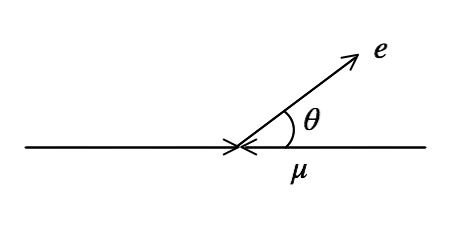
\includegraphics[width=0.75\textwidth]{images/web_feynman/image_21.png}
    \caption[Angle between $e$ and $\mu$ in $e-\mu$ scattering]{Definition of the angle between the electron and muon in the scattering process, $\theta$.}
    \label{fig:ch7_EMuToEMuScatterAngle}
  \end{center}
\end{figure}

In the centre of mass system:

\begin{eqnarray*}
  \sqrt{s} & = & \left(E_D + E_D\right) \\
  & = & \sqrt{p_C^2 + m_C^2} + \sqrt{p_D^2 + m_D^2} \\
  & = & \sqrt{p_C^2 + m_C^2} + \sqrt{p_C^2 + m_D^2} \\
  \Rightarrow \mathrm{d}\sqrt{s} & = & \frac{2p_C\mathrm{d}p_C}{2\sqrt{p_C^2 + m_C^2}} + \frac{2p_C\mathrm{d}p_C}{2\sqrt{p_C^2 + m_D^2}} \\
  & = & p_C \mathrm{d}p_C\left(\frac{1}{\sqrt{p_C^2 + m_C^2}} + \frac{1}{\sqrt{p_D^2 + m_D^2}}\right) \\
  & = & p_C\mathrm{d}p_C\left(\frac{1}{E_C} + \frac{1}{E_D}\right) \\
  & = & p_C\left(\frac{E_D + E_C}{E_DE_C}\right)\mathrm{d}p_C \\
  & = & \frac{p_C\sqrt{s}\mathrm{d}p_C}{E_CE_D} \\
  \Rightarrow \mathrm{d}Q & = & \frac{V^2}{4\pi^2}\delta(\sqrt{s}-\left(E_C + E_D\right))\frac{1}{4}\mathrm{d}\Omega\frac{1}{E_CE_D}p_C^2\mathrm{d}p_C \\
  & = & \frac{V^2}{4\pi^2}\delta\left(\sqrt{s}-\left(E_C+E_D\right)\right)\frac{1}{4}\mathrm{d}\Omega\frac{p_C}{\sqrt{s}}\sqrt{s} \\
  & = & \frac{V^2}{16\pi^2}\mathrm{d}\Omega\frac{\mathrm{d}p_C}{\sqrt{s}} \\
  \Rightarrow \mathrm{d}\sigma & = & \frac{\e^4}{q^4}\frac{1}{V^4}\Big[\left(p_A + p_C\right)_{\mu}\left(p_B + p_D\right)^{\mu}\Big]^2\mathrm{d}Q\frac{V^2}{4p_A\sqrt{s}} \\
  & = & \frac{\e^4}{q^4}\frac{1}{V^4}\Big[\left(p_A + p_C\right)_{\mu}\left(p_B + p_D\right)^{\mu}\Big]\frac{V^2}{4p_A\sqrt{s}}\frac{V^2}{16\pi^2}\mathrm{d}\Omega\frac{p_C}{\sqrt{s}} \\
  \frac{\mathrm{d}\sigma}{\mathrm{d}\Omega} & = & \frac{\e^4}{q^4}\frac{1}{64\pi^2}\frac{\Big[\left(p_A+p_C\right)_{\mu}\left(p_B+p_D\right)^{\mu}\Big]^2p_C}{p_As}
\end{eqnarray*}

The number of final states divided by the flux factor in two body processes is used in many calculations and is:

\[
  \frac{1}{64\pi^2s}\frac{p_C}{p_A}
\]

Consider the cross-section for the massless limit, $m_i \to 0$ or $E_i \gg m_i$, as shown in figure \ref{fig:ch7_particleScattering}, and the definition of $\theta$ shown in figure \ref{fig:ch7_genericScatterAngle}.

\begin{figure}[!htb]
  \begin{center}
    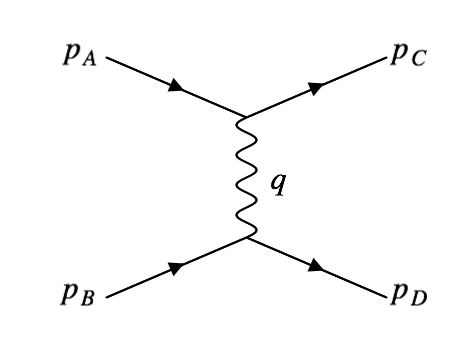
\includegraphics[width=0.5\textwidth]{images/web_feynman/image_22.png}
    \caption[Scattering of massless particles]{Scattering of massless particles.  The momenta are related by $p_A=p_C+q$ and $p_D=p_B+q$.}
    \label{fig:ch7_particleScattering}
  \end{center}
\end{figure}

\begin{figure}[!htb]
  \begin{center}
    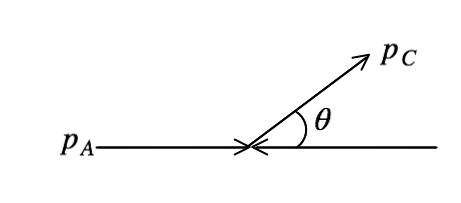
\includegraphics[width=0.75\textwidth]{images/web_feynman/image_23.png}
    \caption[Definition of $\theta$ for a scattering of massless particles]{Definition of $\theta$ for a generic scattering process.}
    \label{fig:ch7_genericScatterAngle}
  \end{center}
\end{figure}

\begin{eqnarray*}
  q^2 & = & \left(p_A - p_C\right)^2 \\
  & = & \left(E_A - E_C,\ul{p}_A - \ul{p}_C\right)^2 \\
  \textrm{For } m \to 0 \quad |\ul{p}_A| & \simeq & E_A \textrm{ etc} \\
  \Rightarrow q^2 & = & \left(E_A - E_C\right)^2 - \left(\ul{p}_A - \ul{p}_C\right)^2 \\
  & = & E_A^2 + E_C^2 - 2E_AE_C - \left(\ul{p}_A - \ul{p}_C\right)^2 \\
  & = & -2E_AE_C + 2\ul{p}_A\cdot\ul{p}_C \\
  & = & -2E_AE_C \left(1 - \cos \theta\right) \\
  \textrm{So } q^4 & = & 4E_A^2E_C^2\left(1 - \cos\theta\right)^2 \\
  \Big[\left(p_A + p_C\right)_{\mu}\left(p_B + p_D\right)^{\mu}\Big]^2 & = & \Big[p_A\cdot p_B + p_A\cdot p_D +p_B\cdot p_C + p_C\cdot p_D \Big]^2 \\
  \textrm{Using } p_A & = & \left(|\ul{p}|,\ul{p} \right) \\
  p_B & = & \left(|\ul{p}|,-\ul{p} \right) \\
  p_C & = & \left(|\ul{p}|,\ul{p}' \right) \\
  p_D & = & \left(|\ul{p}|,-\ul{p}' \right) \\
  \textrm{With } |\ul{p}| & = & |\ul{p}'| \\
  \Rightarrow \Big[\left(p_A + p_C\right)_{\mu}\left(p_B + p_D\right)^{\mu}\Big]^2 & = & \left(6p^2 + 2p^2\cos\theta\right)^2 \\
  \Rightarrow \left(\frac{\mathrm{d}\sigma}{\mathrm{d}\Omega}\right)_{e\mu} & = & \frac{\e^4}{64\pi^4s}\left(\frac{3 + \cos\theta}{1 - \cos\theta}\right)^2
\end{eqnarray*}

\subsection{Note on decay}

Consider the number of states per flux factor for the decay $A \to B \quad C$.

The number of states is as before:

\[
  \frac{1}{16\pi^2}\frac{p_CV^2}{m_A}\mathrm{d}\Omega
\]

Due to the choice of normalisation there are $2E_m$ particles per state in the centre of mass frame in a volume $V$:

\[
  \rho = \frac{2m_A}{V}
\]

The flux factor is:

\begin{eqnarray*}
  F & = & \frac{1}{16\pi^2}\frac{p_CV^2}{m_A}\mathrm{d}\Omega\frac{V}{2m_A} \\
    & = & \frac{1}{32\pi^2}\frac{p_C}{m_A^2}V^3\mathrm{d}\Omega
\end{eqnarray*}

The decay rate is:

\[
  \frac{\mathrm{d}\Gamma}{\mathrm{d}\Omega} = |T_{fi}|^2\frac{1}{32\pi^2}\frac{p_C}{m_A^2}V^3\mathrm{d}\Omega
\]


This factor is universal for decays if the decay is istropic:

\begin{eqnarray*}
  \mathrm{d}\Omega & \to & 4\pi \\
  \mathrm{d}\Gamma & \to & \Gamma
\end{eqnarray*}

For the decay of $A$:

\[
  \frac{\mathrm{d}N_A}{\mathrm{d}t} = \Gamma N_A
\]

ie $N_A(t) = N_A(0)e^{-\Gamma t}$ and $\Gamma^{-1}$ is the mean lifetime.

\cleardoublepage
\chapter{Relativistic spin\texorpdfstring{$-\frac{1}{2}$}{-1Over2} particles (Dirac equation)}
\chaptermark{Relativistic spin$-\frac{1}{2}$ particles}

\section{Non-relativistic description}

There are two spin states, up ($\frac{1}{2}$) and down ($-\frac{1}{2}$).  In spin space there are spin operators given by:

\[
  \bar{s} = \frac{\hbar}{2}\bar{\sigma}
\]

where $\bar{\sigma}$ are the so-called Pauli matrices.  The spin algebra is the same as that of orbital angular momentum.:

\[
  L^2 = l(l+1)\hbar^2
\]

In angular spin momentum:

\[
  S^2 = s(s+1)\hbar^2
\]

The Pauli matrices are:

\begin{eqnarray*}
  \bar{\sigma}_x & = &
  \left(
    \begin{array}{cc}
    0 & 1 \\
    1 & 0
    \end{array}
  \right)
  \\
  \bar{\sigma}_y & = &
  \left(
    \begin{array}{cc}
    0 & -i \\
    i & 0
    \end{array}
  \right)
  \\
  \bar{\sigma}_z & = &
  \left(
    \begin{array}{cc}
    1 & 0 \\
    0 & -1
    \end{array}
  \right)
  \\
  \textrm{where } \bar{I} & = & \bar{\sigma}_x^2 = \bar{\sigma}_y^2 = \bar{\sigma}_z^2
\end{eqnarray*}

The communtation relations are: \nopagebreak

\begin{eqnarray*}
  [\bar{s}_x,\bar{s}_y] & = & i\hbar \bar{s}_z \\
  \textrm{ie} \Bigg[ \frac{\hbar}{2}\bar{\sigma}_x,\frac{\hbar}{2}\bar{\sigma}_y \Bigg] & = & i\left(\frac{\hbar}{2}\right)^2\bar{\sigma}_z
\end{eqnarray*}

Or generally:

\[
  \Big[\bar{\sigma}_i,\bar{\sigma}_j\Big] = 2i\epsilon_{ijk}\bar{\sigma}_k
\]

where $\epsilon_{ijk}$ is the antisymmetric tensor.

\[
  \epsilon_{ijk} = 
  \Bigg\{
    \begin{array}{cc}
    0  & \textrm{if any index is repeated} \\
    1  & \textrm{for } 123, 231, 312 \\
    -1 & \textrm{for } 132, 321, 213
    \end{array}
\]

Also: $\bar{\sigma}_i\bar{\sigma}_j + \bar{\sigma}_j\bar{\sigma}_i = 2\delta_{ij}\bar{I}$.  This is the anticommutation relation.

\[
  \Rightarrow \bar{\sigma}_i\bar{\sigma}_j = \delta_{ij} \bar{I} + i\epsilon_{ijk}\bar{\sigma}_k
\]

\begin{eqnarray*}
  \textrm{Consider }\bar{\sigma}_i\ul{A}\bar{\sigma}_j\ul{B}_j & = & \ul{A}_i\ul{B}_j\delta_{ij} + i\epsilon_{ijk}\bar{\sigma}_k\ul{A}_i\ul{B}_j \\
  \textrm{then } \left(\bar{\sigma}\cdot\ul{A}\right)\left(\bar{\sigma}\cdot\ul{B}\right) & = & \ul{A}\cdot\ul{B} + i\bar{\sigma}\cdot\left(\ul{A}\times\ul{B}\right) \\
  & = & \ul{A}\cdot\ul{B} + i
  \Bigg|
    \begin{array}{ccc}
    \bar{\sigma}_x  & \bar{\sigma}_y  & \bar{\sigma}_z  \\
    \ul{A}_x & \ul{A}_y & \ul{A}_z \\
    \ul{B}_x & \ul{B}_y & \ul{B}_z
    \end{array}
  \Bigg|
\end{eqnarray*}

Suppose $\ul{A} = \ul{B} = \ul{p}$, then:

\[
  \left(\bar{\sigma}\cdot\ul{p}\right)\left(\bar{\sigma}\cdot\ul{p}\right) = |\ul{p}|^2
\]

The gyromagnetic ratio of a particle can be (correctly) determined if the expression for the energy is:

\[
  E = V + \frac{\left(\bar{\sigma}\cdot\ul{p}\right)\left(\bar{\sigma}\cdot\ul{p}\right)}{2m}
\]
as opposed to:
\[
  E = V + \frac{p^2}{2m}
\]
and the electromagnetic coupling is included.

Experimentally the gyromagnetically ratio is $g = 2.00232$ and the Dirac equation gives $g = 2$.

\section{The Dirac equation}

To avoid the problem of negative probability in the negative energy if the Klein-Gordon equation, Dirac proposed an equation linear in $\frac{\partial}{\partial t}$:

\[
  H\psi = \left(\bar{\alpha}\cdot\ul{p} + \beta m\right)\psi
\]

where $\bar{\alpha}$ and $\beta$ are $4\times 4$ matrices and solutions for $\psi$ are multi-component objects.  The formulation must be consistent with $E^2\psi = \left(p^2 + m^2\right)\psi$.

\begin{eqnarray*}
  \textrm{If } E\psi & = & \left(\alpha_ip_i + \beta m\right)\psi \\
  \textrm{then } E^2\psi & = & \left(\alpha_ip_i + \beta m\right)\left(\alpha_j p_j + \beta m\right)\psi \\
  & = & \left(\alpha_i\alpha_jp_ip_j + \left(\alpha_i\beta + \beta\alpha_j\right)p_im + \beta^2m^2\right)\psi \\
  & = & \left( \left(\frac{\alpha_i\alpha_j + \alpha_j\alpha_i}{2}p_ip_j + \alpha\left(\alpha_i\beta \beta\alpha_j\right)p_im + \beta^2m^2\right)\right)\psi \\
  \Rightarrow \bar{\alpha}_i\bar{\alpha}_j + \bar{\alpha}_j\bar{\alpha}_i & = & 2\delta_{ij}\bar{I} \\
  \bar{\alpha}\bar{\beta} + \bar{\beta}\bar{\alpha} & = & \bar{0} \\
  \bar{\beta}^2 & = & \bar{I}
\end{eqnarray*}

\begin{itemize}
  \item $\alpha$ and $\beta$ are Hermitian matrices: $\bar{\alpha} = \bar{\alpha}^{\dagger}$, $\bar{\beta} = \bar{\beta}^{\dagger}$.
  \item $\bar{\alpha}_i^2 = \bar{I}$
  \item $\alpha$ and $\beta$ are traceless
\end{itemize}

The proof that $\alpha$ and $\beta$ are traceless is as follows:

\[
  \bar{\alpha}_i\bar{\beta} = -\bar{\beta}\bar{\alpha}_i
\]

Postmultiplying by $\bar{\beta}$ gives:

\begin{eqnarray*}
  \bar{\alpha}_i\bar{\beta}^2 & = & -\bar{\beta}\bar{\alpha}_i\bar{\beta} \\
  \bar{\alpha}_i\bar{I} & = & -\bar{\beta}\bar{\alpha}_i\bar{\beta}
\end{eqnarray*}

Taking the trace:

\[
  Tr\left(\bar{\alpha}_i\right) = -Tr\left(\bar{\beta}\bar{\alpha}_i\bar{\beta}\right)
\]

Moving the elements cyclically:

\begin{eqnarray*}
  Tr\left(\bar{\alpha}_i\right) & = & - Tr\left(\bar{\beta}^2\bar{\alpha}_i\right) \\
  & = & - Tr\left(\bar{\alpha}_i\right) \\
  \textrm{So } Tr\left(\bar{\alpha}_i\right) & = & 0
\end{eqnarray*}

A common choice for $\bar{\alpha}$ and $\bar{\beta}$ is:

\begin{eqnarray*}
  \bar{\alpha}_i & = &
  \left(
    \begin{array}{cc}
    0 & \bar{\sigma}_i \\
    \bar{\sigma}_i & 0
    \end{array}
  \right)
  \\
  \bar{\beta} & = &
  \left(
    \begin{array}{cc}
    \bar{I} & 0 \\
    0 & -\bar{I}
    \end{array}
  \right)
\end{eqnarray*}

where $\bar{\sigma}_i$ are the Pauli matrices and $\bar{I}$ is the identity matrix.

\subsection{The covariant form of the Dirac equation}

\begin{eqnarray*}
  E\psi & = & \left(\bar{\alpha}_i\cdot\ul{p} + \beta m\right) \psi \\
  E & \to & i\frac{\partial}{\partial t} \\
  \ul{p} & \to & -i\ul{\nabla} \\
  \Rightarrow i\frac{\partial}{\partial t}\psi & = & -i \bar{\alpha}\cdot\ul{\nabla}\psi + \beta m\psi \\
\end{eqnarray*}

Premultiplying by $\beta$:

\begin{eqnarray*}
  i\beta \frac{\partial \psi}{\partial t} & = & -i\beta\bar{\alpha}\cdot\ul{\nabla}\psi + \beta^2 m \psi \\
  \textrm{So } i\beta\frac{\partial \psi}{\partial t} & = & -i\beta\bar{\alpha}\cdot\ul{\nabla}\psi + m\psi \\
  \textrm{Let } \gamma^0 & = & \beta \\
  \gamma^k & = & \beta\alpha \\
  i\gamma^0 \frac{\partial \psi}{\partial t} + i\gamma^k \ul{\nabla}\psi - m\psi & = & 0 \\
  \left( i\gamma^0 \frac{\partial}{\partial x^0} + i\gamma^k\frac{\partial}{\partial x^k} - m\right) & = & 0 \\
  \left( i\gamma^{\mu}\partial_{\mu} - m \right)\psi & = & 0 \\
  \textrm{where } \gamma^{\mu} & = & \left( \gamma^0,\ul{\gamma}^k\right) \\
  \partial_{\mu} & = & \left( \frac{\partial}{\partial x^0},\ul{\nabla}\right)
\end{eqnarray*}

$\gamma^0$ is Hermitian, since $\beta$ is Hermitian.  However, $\gamma^k$ is not Hermitian:

\begin{eqnarray*}
  \left(\gamma^k\right)^{\dagger} & = & -\gamma^k \\
  \gamma^k & = & \beta\alpha^k \\
  \left(\gamma\right)^{\dagger} & = & \left(\beta \alpha^k \right)^{\dagger} \\
  & = & \left(\alpha^k\right)^{\dagger}\beta^{\dagger} \\
  & = & \alpha^k\beta \\
  & = & -\beta\alpha^k \\
  & = & -\gamma^k
\end{eqnarray*}

\[
  \left(\gamma^0\right)^2 = \bar{I} \textrm{ as } \beta^2 = \bar{I}
\]

\begin{eqnarray*}
  \left(\gamma^k\right)^2 & = & \gamma^k\gamma^k \\
  & = & \beta\alpha^k\beta\alpha^k \\
  & = & -\beta\alpha^k\alpha^k\beta \\
  & = & -\beta\beta \\
  & = & -I
\end{eqnarray*}

\subsection{Adjoint Dirac equation and conserved current}

Since the Dirac equation is a matrix equation, to obtain the adjoint equation it is necessary to take the Hermitian conjugate and not the complex conjugate.

\begin{eqnarray}
  \left(i\gamma^{\mu}\partial_{\mu} -m \right)\psi & = & 0 \label{eq:dirac} \\
  \textrm{or } \left( i\gamma^0\frac{\partial}{\partial t} + i\gamma^k\frac{\partial}{\partial x^k} - m \right)\psi & = & 0 \nonumber
\end{eqnarray}

Taking the Hermitian conjugate:

\[
  -i\frac{\partial \psi^{\dagger}}{\partial t}\gamma^0 - i\frac{\partial \psi^{\dagger}}{\partial x^k}\left(-\gamma^k\right) - m\psi^{\dagger} = 0
\]

Postmultiply by $\gamma^0$:

\begin{eqnarray*}
  -i\frac{\partial \psi^{\dagger}}{\partial t} + i\frac{\partial \psi^{\dagger}}{\partial x^k}\gamma^k\gamma^0 - m\psi^{\dagger}\gamma^0 & = & 0 \\
  \gamma^0\gamma^k & = & -\gamma^k\gamma^0 \\
  \Rightarrow -i\frac{\partial \psi^{\dagger}}{\partial t} - i\frac{\partial \psi^{\dagger}}{\partial x^k}\gamma^0\gamma^k - m\psi^{\dagger}\gamma^0 & = & 0
\end{eqnarray*}

Defining the adjoint as:

\[
  \bar{\psi} = \psi^{\dagger}\gamma^0
\]

gives: \nopagebreak

\begin{eqnarray}
  -i \frac{\partial \bar{\psi}}{\partial t}\gamma^0 - i \frac{\partial \bar{\psi}}{\partial x^k}\gamma^k -m\bar{\psi} & = & 0 \nonumber \\
  \textrm{or } i\partial_{\mu}\bar{\psi}\gamma^{\mu} + m\bar{\psi} & = & 0 \label{eq:adjointdirac}
\end{eqnarray}
  
Consider $\bar{\psi}\times$(\ref{eq:dirac})$+$(\ref{eq:adjointdirac})$\times\psi$:

\begin{eqnarray*}
  \bar{\psi}\times(\ref{eq:dirac}) & = & \bar{\psi}i\gamma^{\mu}\partial_{\mu}\psi - \bar{\psi}m\psi = 0 \\
  (\ref{eq:adjointdirac})\times\psi & = & i\partial_{\mu}\bar{\psi}\gamma^{\mu}\psi + m\bar{\psi}\psi = 0 \\
  \textrm{So } i\bar{\psi}\gamma^{\mu}\partial_{\mu}\psi + i\partial_{\mu}\bar{\psi}\gamma^{\mu}\psi & = & 0 \\
  \Rightarrow \partial_{\mu} \left(\bar{\psi}\gamma^{\mu}\psi\right) & = & 0
\end{eqnarray*}

So the expression for $j^{\mu}$:

\[
  j^{\mu} = \bar{\psi}\gamma^{\mu}\psi
\]

satisfies the continuity equation.

$j^{\mu}$ is identified as the probability and flux densities $\rho$ and $\ul{j}$.

The probability density is:

\begin{eqnarray*}
  \rho & = & j^0 \\
  & = & \bar{\psi}\psi \\
  & = & \psi^{\dagger}\gamma^0\gamma^0\psi \\
  & = & \psi^{\dagger}\psi \\
  & = & |\psi|^2
\end{eqnarray*}

Hence $\rho$ is always positive.  For the electromagnetic interaction the charge current density is:

\[
  j^{\mu} = -\e\bar{\psi}\gamma^{\mu}\psi
\]

\subsection{Free particle solutions of the Dirac equation}

Consider solutions of the form:

\[
  \psi = u(p)\e^{-ipx}
\]

Substitute $\psi$ into the Dirac equation:

\begin{eqnarray*}
  \left(i\gamma^{\mu}\partial_{\mu} - m\right)u(p)\e^{-ipx} & = & 0 \\
  \left(i\gamma^{\mu}\left(-ip_{\mu}\right)-m\right)u(p)\e^{-ipx} & = & 0 \\
  \left(\gamma^{\mu}p_{\mu} - m\right)u(p)\e^{-ipx} & = & 0 \\
  \textrm{So } \left(\gamma^{\mu}p_{\mu}-m\right)u(p) & = & 0 \\
  \textrm{Define } \gamma^{\mu}p_{\mu} & = & \not{p} \\
  \textrm{So } \left(\not{p} - m\right)u(p) & = & 0
\end{eqnarray*}

To obtain solutions for $u(p)$, write the above in terms of the $\alpha$ and $\beta$ matrices:

\[
  \left(\gamma^0E - \gamma^kp_k - m\right)u(p) = 0
\]

Premultiplying by $\gamma^0$:

\begin{eqnarray*}
  \left(\left(\gamma^0\right)^2E - \gamma^0\gamma^kp_k - \gamma^0m\right)u(p) & = & 0 \\
  \left(IE - \alpha^kp_k -\beta m\right) u(p) & = & 0
\end{eqnarray*}

For a particle at rest, $\ul{p} = \ul{0}$:

\begin{eqnarray*}
  \left(IE - \beta m\right)u(p) & = & 0 \\
  \Rightarrow m
  \left(
    \begin{array}{cc}
    I & 0 \\
    0 & -I
    \end{array}
  \right)
  u(p)
  & = & 
  \left(
    \begin{array}{cc}
    I & 0 \\
    0 & I
    \end{array}
  \right)
  Eu(p)
\end{eqnarray*}

Solutions exist if:

\[
  \Bigg|
    \begin{array}{cc}
    (m - E)I & 0 \\
    0 & -(m + E)I
    \end{array}
  \Bigg|
  = 0
\]

or in longhand:

\begin{eqnarray*}
  \left|
    \begin{array}{cccc}
    m-E & 0 & 0 & 0  \\
    0 & m-E & 0 & 0  \\
    0 & 0 & -m-E & 0 \\
    0 & 0 & 0 & -m-e
    \end{array}
  \right|
  & = & 0 \\
  \Big[\left(m-E\right)\left(m+E\right)\Big]^2 & = & 0
\end{eqnarray*}

So there are four eigenvalues corresponding to $E = \pm m$ in two coincident pairs.  This means that negative energy solutions still exist.  $u_1, u_2$ are associated with positive energy solutions and $u_3, u_4$ are associated with negative energy solutions.

Consider the solutions when $\ul{p} \neq \ul{0}$.  From $\left(\bar{\alpha}\cdot\ul{p} + \beta m\right)u = 0$:

\[
  \Bigg[
  \left(
    \begin{array}{cc}
    0 & \sigma \\
    \sigma & 0
    \end{array}
  \right)
  \cdot \ul{p}
  +
  \left(
    \begin{array}{cc}
    I & 0 \\
    0 & -I
    \end{array}
  \right)
  m
  \Bigg]
  \left(
    \begin{array}{c}
    u_A \\
    u_B
    \end{array}
  \right)
  = E
  \left(
    \begin{array}{c}
    u_A \\
    u_B
    \end{array}
  \right)
\]

This yields:

\begin{eqnarray}
  \bar{\sigma}\cdot\ul{p} u_B + mu_A & = & Eu_A \label{eq:diracub} \\
  \bar{\sigma}\cdot\ul{p} u_A - mu_B & = & Eu_B \label{eq:diracua}
\end{eqnarray}

\begin{eqnarray*}
  \textrm{From (\ref{eq:diracub}) } & u_A & = \frac{\bar{\sigma}\cdot\ul{p}u_B}{E - m} \\
  \textrm{From (\ref{eq:diracua}) } & u_A & = \frac{\bar{\sigma}\cdot\ul{p}u_A}{E + m}
\end{eqnarray*}

\begin{eqnarray*}
  \textrm{For } E>0: && \\
  u_A & =
  \left(
    \begin{array}{c}
    1 \\
    0
    \end{array}
  \right)
  & \textrm{ (spin up)}
  \\
  \textrm{or} && \\
  u_A & =
  \left(
    \begin{array}{c}
    0 \\
    1
    \end{array}
  \right)
  & \textrm{ (spin down)}
\end{eqnarray*}

\begin{eqnarray*}
  \textrm{So } u_1 & = & N
  \left(
    \begin{array}{c}
    1 \\
    0 \\
    \frac{\bar{\sigma}\cdot\ul{p}}{E + m} \\
    0
    \end{array}
  \right)
  \\
  u_2 & = & N
  \left(
    \begin{array}{c}
    0 \\
    1 \\
    0 \\
    \frac{\bar{\sigma}\cdot\ul{p}}{E + m}
    \end{array}
  \right)
\end{eqnarray*}

where $N$ is a normalisation constant.

For $E<0$:

\begin{eqnarray*}
  u_A & = & \frac{\bar{\sigma}\cdot\ul{p}}{E - m}u_B \\
  & = & \frac{\bar{\sigma}\cdot\ul{p}}{-|E| - m}u_B \\
  & = & -\frac{\bar{\sigma}\cdot\ul{p}}{|E| + m}u_B
\end{eqnarray*}

\begin{eqnarray*}
  \textrm{So } u_3 & = & N
  \left(
    \begin{array}{c}
    -\frac{\bar{\sigma}\cdot\ul{p}}{|E| + m} \\
    0 \\
    1 \\
    0
    \end{array}
  \right)
  \\
  u_4 & = & N
  \left(
    \begin{array}{c}
    0 \\
    -\frac{\bar{\sigma}\cdot\ul{p}}{E + m} \\
    0 \\
    1
    \end{array}
  \right)
\end{eqnarray*}

In summary all the above comes from:

\[
  \left( \not{p} - m \right) = 0
\]

with the propagation factor $\e^{-ipx}$.

Now associate negative energy solutions ($u_3,u_4$) such that they describe positron solutions propagating backwards in time with the propagation factor $\e^{ipx}$:

\begin{eqnarray*}
  u^{(3,4)}(-p)\e^{-i(-p)x} & = v^{(2,1)}(p)\e^{ipx} \\
  \Rightarrow v_2 & =
  \left(
    \begin{array}{c}
    \frac{\bar{\sigma}\cdot\ul{p}}{E + m} \\
    0 \\
    1 \\
    0
    \end{array}
  \right)
  & \textrm{ (spin down)}
  \\
  v_1 & =
  \left(
    \begin{array}{c}
    0 \\
    \frac{\bar{\sigma}\cdot\ul{p}}{E + m} \\
    0 \\
    1
    \end{array}
  \right)
  & \textrm{ (spin up)}
\end{eqnarray*}

The original equation for an electron of energy $-E$ and momentum $-\ul{p}$ is:

\begin{eqnarray*}
  \left(-\not{p} - m\right)u(-p) & = & 0 \\
  \Rightarrow \left(\not{p} + m\right)v(p) & = & 0
\end{eqnarray*}

\subsection{Orthogonality and normalisation of spinors}

\begin{eqnarray*}
  \psi_1 & = & N
  \left(
    \begin{array}{c}
    1 \\
    0 \\
    \frac{\bar{\sigma}\cdot\ul{p}}{E + m} \\
    0
    \end{array}
  \right)
  \e^{-ipx}
  \\
  \psi_2 & = & N
  \left(
    \begin{array}{c}
    0 \\
    1 \\
    0 \\
    \frac{\bar{\sigma}\cdot\ul{p}}{E + m}
    \end{array}
  \right)
  \e^{-ipx}
\end{eqnarray*}

For orthogonality:

\begin{eqnarray*}
  \int \psi_1^{\dagger}\psi_2\mathrm{d}^3x & = & 0 \\
  \Rightarrow N^{\star}N\left(1 0 \frac{\left(\bar{\sigma}\cdot\ul{p}\right)^{\dagger}}{E + m} 0\right)
  \left(
    \begin{array}{c}
    0 \\
    1 \\
    0 \\
    \frac{\bar{\sigma}\cdot\ul{p}}{E + m} 
    \end{array}
  \right)
  & = & 0
\end{eqnarray*}

So $\psi_1$ and $\psi_2$ are orthogonal to each other.  Similarly $\psi_3$ and $\psi_4$ are orthogonal to each other.

In order to normalise to $2E$ particles in a volume $V$:

\begin{eqnarray*}
  \int \psi_1^{\dagger}\psi_1\mathrm{d}^3x & = & 2E \\
  \Rightarrow \int N^{\star}N\left( 1 \quad 0 \quad \left(\frac{\bar{\sigma}\cdot\ul{p}}{E + m}\right)^{\dagger} \quad 0 \right)
  \left(
    \begin{array}{c}
    1 \\
    0 \\
    \frac{\bar{\sigma}\cdot\ul{p}}{E + m} \\
    0
    \end{array}
  \right)
  \mathrm{d}^3x & = & 2E
  \\
  \Rightarrow \int N^{\star}N\Bigg[ 1 + \left( \frac{\bar{\sigma}\cdot\ul{p}}{E + m} \right)^2 \Bigg]\mathrm{d}^3x & = & 2E \\
  \textrm{where } \left(\bar{\sigma}\cdot\ul{p}\right)^{\dagger} & = & \bar{\sigma}\cdot\ul{p}
\end{eqnarray*}

\begin{eqnarray*}
  \bar{\sigma}_y & = &
  \left(
    \begin{array}{cc}
    0 & -i \\
    i & 0
    \end{array}
  \right)
  \\
  \Rightarrow
  \left(
  \bar{\sigma}_y\cdot\ul{p}_y\right)^2 & = &
  \left(
    \begin{array}{cc}
    0 & -ip_y \\
    ip_y & 0
    \end{array}
  \right)^2
  \\
  & = &
  \left(
    \begin{array}{cc}
    p_y^2 & 0 \\
    0 & p_y^2
    \end{array}
  \right)
  \\
  & = & p_y^2 \bar{I}
\end{eqnarray*}

\begin{eqnarray*}
  \textrm{So } \int N^{\star}N\left( 1 + \frac{p^2}{\left(E + m\right)^2}\right)\mathrm{d}^3x & = & 2E \\
  \Rightarrow N^{\star}N\left(\frac{\left(E + m\right)^2 + E^2 - m^2}{\left(E + m\right)^2}\right)\mathrm{d}^3x & = & 2E \\
  & = & \int N^{\star}N\frac{2E}{E + m}\mathrm{d}^3 x \\
  \textrm{So } \frac{N^{\star}NV}{E + m} & = & 1 \\
  \Rightarrow N & = & \sqrt{\frac{E + m}{V}}
\end{eqnarray*}

\subsection{Spin}

Neither the orbital angular momentum nor the spin angular momentum commute with the Dirac Hamiltonian, but $J = L + S$ does commute.  To find an operator other than $J$ that commutes with the Dirac Hamiltonian recall the Dirac equation:

\[
  H
  \left(
    \begin{array}{c}
    u_A \\
    u_B
    \end{array}
  \right)
  =
  \left(\bar{\alpha}\cdot\ul{p} + \beta m\right)
  \left(
    \begin{array}{c}
    u_A \\
    u_B
    \end{array}
  \right)
\]

$\bar{\alpha}\cdot\ul{p} + \beta m$ is the Dirac Hamiltonian.

\begin{eqnarray*}
  H
  \left(
    \begin{array}{c}
    u_A \\
    u_B
    \end{array}
  \right)
  & = &
  E
  \left(
    \begin{array}{c}
    u_A \\
    u_B
    \end{array}
  \right)
  \\
  & = &
  \left(
    \begin{array}{cc}
    m\bar{I} & \bar{\sigma}\cdot\ul{p}\bar{I} \\
    \bar{\sigma}\cdot\ul{p}\bar{I} & -m\bar{I}
    \end{array}
  \right)
  \left(
    \begin{array}{c}
    u_A \\
    u_B
    \end{array}
  \right)
\end{eqnarray*}

By inspection, the Dirac Hamiltonian commutes with $\bar{\sigma}\cdot\ul{p}\bar{I}$:

\[
\left(
  \begin{array}{cc}
  m\bar{I} & \bar{\sigma}\cdot\ul{p}\bar{I} \\
  \bar{\sigma}\cdot\ul{p}\bar{I} & -m\bar{I}
  \end{array}
\right)
\left(
  \begin{array}{cc}
  \bar{\sigma}\cdot\ul{p}\bar{I} & 0 \\
  0 & \bar{\sigma}\cdot\ul{p}\bar{I}
  \end{array}
\right)
  -
  \left(
    \begin{array}{cc}
    \bar{\sigma}\cdot\ul{p}\bar{I} & 0 \\
    0 & \bar{\sigma}\cdot\ul{p}\bar{I}
    \end{array}
  \right)
  \left(
    \begin{array}{cc}
    m\bar{I} & \bar{\sigma}\cdot\ul{p}\bar{I} \\
    \bar{\sigma}\cdot\ul{p}\bar{I} & m\bar{I}
    \end{array}
  \right)
  =
  \left(
    \begin{array}{cc}
    0 & 0 \\
    0 & 0
    \end{array}
  \right)
\]

Define the helicity operator as: 

\[
  H = \frac{1}{2}\bar{\sigma}\cdot\ul{\hat{p}} = \frac{1}{2} \frac{\bar{\sigma}\cdot\ul{p}}{|\ul{p}|}
\]

The helicity is the projection of the spin along the direction of motion and its eigenvalues are $\pm \frac{1}{2}$.  $H = \frac{1}{2}$ corresponds to positive helicity and $H = \frac{-1}{2}$ corresponds to negative helicity.

\begin{figure}[!htb]
  \begin{center}
    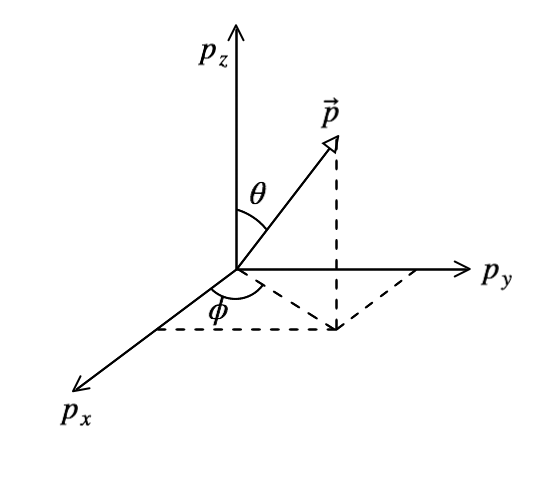
\includegraphics[width=0.75\textwidth]{images/web_feynman/image_24.png}
    \caption[Projection of momentum in three dimensions]{Projection of momentum in three dimensions.}
    \label{fig:ch8_momentum}
  \end{center}
\end{figure}

Suppose a particle has a momentum $\ul{p}$, with coordinates defined in figure \ref{fig:ch8_momentum}, where:

\begin{eqnarray*}
  \ul{\hat{p}} & = & \sin\theta\cos\phi\hat{\ul{i}} + \sin\theta\sin\phi\hat{\ul{j}} + \cos\theta\hat{\ul{k}} \\
  \bar{\sigma}\cdot\ul{\hat{p}} & = & \bar{\sigma}_x\cdot\ul{\hat{p}}_x + \bar{\sigma}_y\cdot\ul{\hat{p}}_y + \bar{\sigma}_z\cdot\ul{\hat{p}}_z \\
  & = &
  \left(
    \begin{array}{cc}
    0 & 1 \\
    1 & 0
    \end{array}
  \right)
  \sin\theta\cos\phi
  +
  \left(
    \begin{array}{cc}
    0 & -i \\
    i & 0
    \end{array}
  \right)
  \sin\theta\sin\phi
  +
  \left(
    \begin{array}{cc}
    1 & 0 \\
    0 & -1
    \end{array}
  \right)
  \cos\theta
  \\
  \textrm{So } \frac{1}{2}\bar{\sigma}\cdot\ul{\hat{p}}
  \left(
    \begin{array}{c}
    u_A \\
    u_B
    \end{array}
  \right)
  & = & \frac{1}{2}
  \left(
    \begin{array}{cc}
    \cos\theta & \sin\theta \e^{-i\phi} \\
    \sin\theta \e^{i\phi} & -\cos\theta
    \end{array}
  \right)
  \left(
    \begin{array}{c}
    u_A \\
    u_B
    \end{array}
  \right)
\end{eqnarray*}

So the eigenvalue equation is:

\begin{eqnarray*}
  \frac{1}{2}
  \left(
    \begin{array}{cc}
    \cos\theta & \sin\theta \e^{-i\phi} \\
    \sin\theta\e^{i\phi} & -\cos\theta
    \end{array}
  \right)
  \left(
    \begin{array}{c}
    u_A \\
    u_B
    \end{array}
  \right)
  & = & \lambda
  \left(
    \begin{array}{c}
    u_A \\
    u_B
    \end{array}
  \right)
  \\
  \Bigg|
    \begin{array}{cc}
    \cos\theta - 2\lambda & \sin\theta\e^{-i\phi} \\
    \sin\theta\e^{i\phi} & -\cos\theta - 2\lambda
    \end{array}
  \Bigg|
  & = & 0 \\
  \left(-\cos\theta-2\lambda\right)\left(\cos\theta+2\lambda\right) - \sin^2\theta & = & 0 \\
  -\cos^2\theta + 4\lambda^2 - \sin^2\theta & = & 0 \\
  \Rightarrow \lambda & = & \pm\frac{1}{2}
\end{eqnarray*}

\subsection{The \texorpdfstring{$\gamma^5$}{G5} matrix}

The $\gamma^5$ matrix is used to simplify notation:

\[
  \gamma^5 = i\gamma^0\gamma^1\gamma^2\gamma^3
\]

$\gamma^5$ has many properties:

\begin{eqnarray*}
  \left(\gamma^5\right)^{\dagger} & = & \gamma^5 \\
  \left(\gamma^5\right)^2 & = & \bar{I} \\
  \gamma^5\gamma^{\mu} + \gamma^{\mu}\gamma^5 & = & 0
\end{eqnarray*}

Ãn Dirac-Pauli representation:

\begin{eqnarray*}
  \gamma^0 & = &
  \left(
    \begin{array}{cc}
    \bar{I} & \bar{0} \\
    \bar{0} & \bar{I}
    \end{array}
  \right)
  \\
  \gamma^k & = &
  \left(
    \begin{array}{cc}
    \bar{0} & \bar{\sigma}_k \\
    \bar{\sigma}_k & \bar{0}
    \end{array}
  \right)
  \\
  \gamma^5 & = &
  \left(
    \begin{array}{cc}
    \bar{0} & \bar{I} \\
    \bar{I} & \bar{0}
    \end{array}
  \right)
\end{eqnarray*}

Consider the effect of $\gamma^5$ operating upon the Dirac equation (dropping the bars that signify matrices):

\begin{eqnarray*}
  \gamma^5
  \left(
    \begin{array}{c}
    u_A \\
    u_B
    \end{array}
  \right)
  & = &
  \left(
    \begin{array}{cc}
    0 & I \\
    I & 0
    \end{array}
  \right)
  \left(
    \begin{array}{c}
    \chi \\
    \left(\frac{\sigma\cdot p}{E + m}\right)\chi
    \end{array}
  \right)
  \\
  \textrm{where }\chi & = &
  \left(
    \begin{array}{c}
    1 \\
    0
    \end{array}
  \right)
  \\
  \gamma^5
  \left(
    \begin{array}{c}
    u_A \\
    u_B
    \end{array}
  \right)
  & = &
  \left(
    \begin{array}{c}
    \left(\frac{\sigma\cdot p}{E + m}\right)\chi \\
    \chi
    \end{array}
  \right)
\end{eqnarray*}

For high energies, or in the limit $m \to 0$, $E \sim p$:

\begin{eqnarray*}
  \gamma^5
  \left(
    \begin{array}{c}
    u_A \\
    u_B
    \end{array}
  \right)
  & \simeq &
  \left(
    \begin{array}{c}
    \sigma\cdot\hat{p} \chi \\
    \chi
    \end{array}
  \right)
  \\
  & = &
  \left(
    \begin{array}{c}
    \sigma\cdot\hat{p}\chi \\
    I\chi
    \end{array}
  \right)
  \\
  & = & 
  \left(
    \begin{array}{c}
    \sigma\cdot\hat{p}\chi \\
    \left(\sigma\cdot\hat{p}\right)^2\chi
    \end{array}
  \right)
  \\
  & = &
  \sigma\cdot\hat{p}
  \left(
    \begin{array}{c}
    \chi \\
    \sigma\cdot\hat{p}\chi
    \end{array}
  \right)
  \\
  & = &
  \sigma\cdot\hat{p}
  \left(
    \begin{array}{c}
      \chi \\
      \left(\frac{\sigma\cdot\ p}{E + m}\right)\chi
    \end{array}
  \right)
  \\
  & = &
  \sigma\cdot\hat{p}
  \left(
    \begin{array}{c}
    u_A \\
    u_B
    \end{array}
  \right)
  \\
  \textrm{So }\gamma^5
  \left(
    \begin{array}{c}
    u_A \\
    u_B
    \end{array}
  \right)
  & = &
  \left(
    \begin{array}{cc}
    \sigma\cdot\hat{p} & 0 \\
    0 & \sigma\cdot\hat{p}
    \end{array}
  \right)
  \left(
    \begin{array}{c}
    u_A \\
    u_B
    \end{array}
  \right)
\end{eqnarray*}

So in the limit $m \to 0$, $\gamma^5$ becomes the helicity operator.

Operators can then be defined as follows:

\begin{eqnarray*}
  P_R & = & \frac{1}{2}\left(1 + \gamma^5\right) \\
  P_L & = & \frac{1}{2}\left(1 - \gamma^5\right)
\end{eqnarray*}

These operators are then respectively the left and right-handed projection operators of helicity.

Where $m\neq 0$ (which is generally the case) the operator $\frac{1}{2}\left(1 + \gamma^5\right)$ is the right-handed chirality state and if $m$ is small then the state can be approximated as a right-handed helicity state, but will also contain a small fraction of the left-handed helicity component.

\subsection{Completeness relation}

The completeness relations are used extensively in the evaluation of Feynmann diagram calculations.

Consider the summation over all spin states:

\begin{eqnarray*}
  \sum_{S = 1,2} u_s(p)\bar{u}_s(p) & = &  \sum_{S = 1,2} N^{\star}N
  \left(
    \begin{array}{c}
    \chi_S \\
    \frac{\sigma \cdot p}{E + m}\chi_S
    \end{array}
  \right)
  \left( \chi_S^{\dagger} , -\frac{\sigma\cdot p}{E + m}\chi^{\dagger} \right) \\
  & = & \sum_{S = 1,2} N^{\star}N
  \left(
    \begin{array}{cc}
    \chi_S^{\dagger}\chi & -\frac{\left(\sigma\cdot p\right)^{\dagger}}{E + m}\chi_S^{\dagger}\chi_S \\
    \frac{\sigma\cdot p}{E + m}\chi_S^{\dagger}\chi_S & -\frac{E^2 - m^2}{\left(E + m\right)^2}\chi_S^{\dagger}\chi_S
    \end{array}
  \right)
  \\
  & = & \sum_{S = 1,2}N^{\star}N
  \left(
    \begin{array}{cc}
    I & -\frac{\left(\sigma\cdot p\right)^{\dagger}}{E + m} \\
    \frac{\sigma\cdot p}{E + m} & -\frac{E^2 - m^2}{\left(E + m\right)^2}
    \end{array}
  \right)
  \chi_S^{\dagger}\chi
\end{eqnarray*}

The summation over states is:

\begin{eqnarray*}
  \sum_{S = 1,2} \chi_S^{\dagger}\chi_S & = &
  \left(
    \begin{array}{c}
    1 \\
    0
    \end{array}
  \right)
  \left(1 0\right)
  +
  \left(
    \begin{array}{c}
    0 \\
    1
    \end{array}
  \right)
  \left(0 1\right)
  \\
  & = &
  \left(
    \begin{array}{cc}
    1 & 0 \\
    0 & 1
    \end{array}
  \right)
\end{eqnarray*}

\[
  N^{\star}N = E + m
\]

\begin{eqnarray}
  \sum_{S = 1,2} u_S\bar{u}_S & = &
  \left(
    \begin{array}{cc}
    I & -\frac{\sigma\cdot p}{E + m} \\
    \frac{\sigma \cdot p}{E + m} & -\frac{E^2 - m^2}{\left(E + m\right)^2}I
    \end{array}
  \right)
  \left(E + m\right)
  \nonumber
  \\
  & = &
  \left(
    \begin{array}{cc}
    \left(E + m\right)I & -\sigma\cdot p \\
    \sigma\cdot p & -I\left(E - m\right)
    \end{array}
  \right)
  \nonumber
  \\
  & = &
  \left(
    \begin{array}{cc}
    \left(E + m\right)I & -\sigma\cdot p \\
    \sigma\cdot p & \left(m - E\right)I
    \end{array}
  \right)
  \label{eq:completeness1}
  \\
  \textrm{However } \not{p} + m & = & \gamma^{\mu}p_{\mu} + mI \nonumber \\
  & = & \gamma^0E - \gamma^kp_k + mI \nonumber \\
  & = &
  \left(
    \begin{array}{cc}
    I & 0 \\
    0 & -I
    \end{array}
  \right)
  E -
  \left(
    \begin{array}{cc}
    0 & \sigma_k \\
    -\sigma_k & 0
    \end{array}
  \right)
  p_k +
  \left(
    \begin{array}{cc}
    I & 0 \\
    0 & I
    \end{array}
  \right)
  m
  \nonumber
  \\
  & = &
  \left(
    \begin{array}{cc}
    \left(E + m\right) I & -\sigma\cdot p \\
    \sigma\cdot p & \left(m - E\right) I
    \end{array}
  \right)
  \label{eq:completeness2}
\end{eqnarray}

So (\ref{eq:completeness1})$ = $(\ref{eq:completeness2}).

\begin{eqnarray*}
  \sum_{S = 1,2} u_S\bar{u}_S & = & \not{p} + m \\
  \sum_{S = 1,2} v_S\bar{v}_S & = & \not{p} - m
\end{eqnarray*}

\subsection{Possible forms of interaction}

An exhasutive set of possibilities of interaction is:

\paragraph*{Scalar interactions} $\bar{u}u$ (even parity)
\paragraph*{Vector interactions} $\bar{u}\gamma^{\mu}u$ (odd parity)  This interaction causes allowed Fermi transitions in $\beta$ decay and in $\mu$ decay.  
\paragraph*{Tensor interactions} $\bar{u}\sigma^{\mu\nu}u$  As far as has been confirmed by experiment this interaction does not exist, except for anomalous magnetic moments.
\paragraph*{Axial vector interactions} $\bar{u}\gamma^5\gamma^{\mu}u$ (even parity)  The weak interaction is a mixture of the vector and axial vector interactions.  In some nuclei, either the vector or axial vector process cannot take place.  In many $\beta$ decays of nuclei both of the processes take place.
\paragraph*{Pseudoscalar interactions} $\bar{u}\gamma^5u$ (odd parity)

\section{Trace theorems}

\subsection{\texorpdfstring{$Tr[I]$}{TrI}}

\[
  Tr[I] = 4
\]

\subsection{\texorpdfstring{$Tr[\not{a}\not{b}]$}{TrNotANotB}}

\begin{eqnarray*}
  Tr[\not{a}\not{b}] & = & Tr[\not{b}\not{a}] \\
  \textrm{So } Tr[\not{a}\not{b}] & = & \frac{1}{2}Tr[\not{a}\not{b} + \not{b}\not{a}] \\
  & = & \frac{1}{2} Tr[\gamma^{\mu}\gamma^{\nu}a_{\mu}b_{\nu} + \gamma^{\mu}\gamma^{\nu}b_{\mu}a_{\nu}] \\
  \gamma^{\mu}\gamma{^\nu} + \gamma^{\nu}\gamma^{\mu} & = & 2g^{\mu\nu}I \\
  & = & \frac{1}{2}a\cdot b 2 Tr[I] \\
  & = & 4a\cdot b
\end{eqnarray*}

\subsection{\texorpdfstring{$Tr[\not{a}\not{b}\not{c}\not{d}]$}{TrNotANotBNotCNotD}}

\begin{eqnarray*}
  Tr[\not{a}\not{b}\not{c}\not{d}] & = & Tr[\gamma^{\mu}\gamma^{\nu}\gamma^{\delta}\gamma^{\sigma}a_{\mu}b_{\nu}c_{\delta}d_{\sigma}] \\
  \textrm{But } Tr[\gamma^{\mu}\gamma{\nu}\gamma{\delta}\gamma^{\sigma}] & = & - Tr[\gamma^{\nu}\gamma^{\mu}\gamma^{\delta}\gamma^{\sigma}] + Tr[2g^{\mu\nu}\gamma{\delta}{\sigma}] \\
  & = & Tr[\gamma^{\nu}\gamma^{\delta}\gamma^{\mu}\gamma^{\sigma}] - Tr[2g^{\mu\delta}\gamma^{\nu}\gamma^{\sigma}] + Tr[2g^{\mu\nu}\gamma^{\delta}\gamma^{\sigma}] \\
  & = & -Tr[\gamma^{\nu}\gamma^{\delta}\gamma^{\sigma}\gamma^{\mu}] + Tr[2g^{\mu\sigma}\gamma^{\nu}\gamma^{\delta}] - Tr[2g^{\mu\delta}\gamma^{\nu}\gamma^{\sigma}] + Tr[2g^{\mu\nu}\gamma^{\delta}\gamma^{\sigma}] \\
  \Rightarrow Tr[\gamma^{\mu}\gamma^{\nu}\gamma^{\delta}\gamma^{\sigma}] & = & Tr[g^{\mu\sigma}\gamma^{\nu}\gamma^{\delta}] - Tr[g^{\mu\delta}\gamma^{\nu}\gamma^{\sigma}] + Tr[g^{\mu\nu}\gamma^{\delta}\gamma^{\sigma}] \\
  Tr[\gamma^{\mu}\gamma^{\nu}] & = & 4g^{\mu\nu} \\
  Tr[\gamma^{\mu}\gamma^{\nu}\gamma^{\delta}\gamma^{\sigma}] & = & 4\left(g^{\mu\sigma}g^{\nu\delta} - g^{\mu\delta}g^{\nu\sigma} + g^{\mu\nu}g^{\delta\sigma} \right) \\
  \Rightarrow Tr[\gamma^{\mu}\gamma^{\nu}\gamma^{\delta}\gamma^{\sigma}]a_{\mu}b_{\nu}c_{\delta}d_{\sigma} & = & 4\Big[ (a\cdot d)(b\cdot c) - (a\cdot c)(b\cdot d) + (a\cdot b)(c\cdot d)\Big]
\end{eqnarray*}

Some other identities, which shall be used in the calculation of the cross-section for Compton scattering include:

\subsection{\texorpdfstring{$\gamma_{\mu}\gamma^{\nu}\gamma^{\mu} = -2\gamma^{\nu}$}{GMuGNuGMu}}

\begin{eqnarray*}
  \gamma_{\mu}\gamma^{\nu}\gamma^{\mu} & = & -\gamma_{\mu}\gamma^{\mu}\gamma^{\nu} + 2g^{\mu\nu}\gamma_{\mu} \\
  & = & -4\gamma^{\nu} + 2\gamma^{\nu} \\
  & = & -2\gamma^{\nu} \\
  \textrm{or } \gamma_{\mu}\not{a}\gamma^{\mu} & = & -2\not{a}
\end{eqnarray*}

\subsection{\texorpdfstring{$\gamma_{\mu}\gamma^{\delta}\gamma^{\sigma}\gamma^{\mu} = 4 g^{\delta\sigma}$}{GMuGDeltaGSigmaGMu}}

\begin{eqnarray*}
  \gamma_{\mu}\gamma^{\delta}\gamma^{\sigma}\gamma^{\mu} & = & -\gamma{\delta}\gamma_{\mu}\gamma^{\sigma}\gamma^{\mu} + 2g_{\mu\delta}\gamma^{\sigma}\gamma^{\mu} \\
  & = & 2\gamma^{\delta}\gamma^{\sigma} + 2\gamma^{\sigma}\gamma^{\delta} \\
  & = & 4g^{\delta\sigma} \\
  \textrm{or } \gamma_{\mu}\not{a}\not{b}\gamma^{\mu} & = & 4 a\cdot b
\end{eqnarray*}

\subsection{\texorpdfstring{$\gamma_{\mu}\not{a}\not{b}\not{c}\gamma^{\mu} = -2\not{c}\not{b}\not{a}$}{GMuNotANotBNotCGMu}}

\begin{eqnarray*}
  \gamma_{\mu}\not{a}\not{b}\gamma^{\nu}\gamma^{\mu}c_{\nu} & = & -\gamma_{\mu}\not{a}\not{b}\gamma^{\mu}\gamma^{\nu}c_{\nu} + \gamma_{\mu}\not{a}\not{b}2g^{\nu\mu}c_{\nu} \\
  & = & -4(a\cdot b) \not{c} + 2\not{c}\not{a}\not{b} \\
  & = & -4(a\cdot b) \not{c} + 2\not{c}\gamma^{\alpha}\gamma^{\beta}a_{\alpha}b_{\beta} \\
  & = & -4(a\cdot b) \not{c} - 2\not{c}\gamma^{\beta}\gamma^{\alpha}a_{\alpha}b_{\beta} + 2\not{c}2g^{\alpha\beta}a_{\alpha}b_{\beta} \\
  & = & -2\not{c}\not{b}\not{a}
\end{eqnarray*}

\subsection{\texorpdfstring{$Tr[\gamma^5\gamma^{\mu}] = 0$}{TrG5GMu}}

\begin{eqnarray*}
  \gamma^5\gamma^{\mu} + \gamma^{\mu}\gamma^5 & = & 0 \\
  \Rightarrow Tr[\gamma^5\gamma^{\mu}] & = & -Tr[\gamma^{\mu}\gamma^5] \\
  & = & -Tr[\gamma^5\gamma^{\mu}] \\
  \textrm{So } Tr[\gamma^5\gamma^{\mu}] & = & 0
\end{eqnarray*}

\subsection{\texorpdfstring{$Tr[\gamma^{5}\gamma^{\mu}\gamma^{\nu}] = 0$}{TrG5GMuGNu}}

Assume that $\gamma^{\mu} = \gamma^{\nu}$

\begin{eqnarray*}
  Tr[\gamma^5\left(\gamma^{\mu}\right)^2] & = & Tr (\gamma^5 I) \\
  & = & Tr
  \Bigg[
  \left(
    \begin{array}{cc}
    0 & I \\
    I & 0
    \end{array}
  \right)
  \left(
    \begin{array}{cc}
    I & 0 \\
    0 & I
    \end{array}
  \right)
  \Bigg]
  \\
  & = & 0
\end{eqnarray*}

Now assume $\mu = 1$, $\nu = 2$

\begin{eqnarray*}
  Tr[i\gamma^0\gamma^1\gamma^2\gamma^3\gamma^1\gamma^2] & = & Tr[i\gamma^0\left(\gamma^1\right)^2\gamma^2\gamma^3\gamma^2 ] \\
  & = & -Tr[i\gamma^0\left(\gamma^2\right)^2\gamma^3] \\
  & = & -iTr[\gamma^0\gamma^3] \\
  & = & -iTr[\gamma^3\gamma^0] \\
  \textrm{and } Tr[\gamma^0\gamma^3 + \gamma^3\gamma^0] & = & 2Tr[g^{03}I] \\
  & = & 0 \\
  \Rightarrow Tr[\gamma^3\gamma^0] & = & 0 \\
  \textrm{So } Tr[\gamma^5\gamma^1\gamma^2] & = & 0
\end{eqnarray*}

\subsection{\texorpdfstring{$Tr[\gamma^5\gamma^{\nu}\gamma^{\mu}\gamma^{\delta}] = 0 $}{TrG5GNuGMuGDelta}}

The trace of an odd number of $\gamma$ matrices is zero:

\begin{eqnarray*}
  Tr[\not{a}_1\not{a}_2\cdots\not{a}_n] & = & Tr[\not{a}_a\not{a}_2\cdots\not{a}_n\gamma^5\gamma^5] \\
  \textrm{Back-propagate }\gamma^5: &&\\
  Tr[\not{a}_1\not{a}_2\cdots\not{a}_n] & = & \left(-1\right)^nTr[\gamma^5\not{a}_a\not{a}_2\cdots\not{a}_n\gamma^5] \\
  & = & \left(-1\right)^n Tr[\not{a}_1\not{a}_2\cdots\not{a}_n\gamma^5\gamma^5] \\
  \textrm{as traces are cyclic} &&\\
  \textrm{So } Tr[\not{a}_1\not{a}_2\cdots\not{a}_n & = & \left(-1\right)^nTr[\not{a}_1\not{a}_2\cdots\not{a}_n] \\
\end{eqnarray*}

So as $n$ is odd, the Trace is equal to zero.

\subsection{\texorpdfstring{$Tr[\gamma^5\gamma^{\mu}\gamma^{\nu}\gamma^{\delta}\gamma^{\sigma}]$}{TrG5GMuGNuGDeltaGSigma}}

First consider $Tr[\gamma^5\gamma^0\gamma^1\gamma^2\gamma^3]$:

\begin{eqnarray*}
  Tr[\gamma^5\gamma^0\gamma^1\gamma^2\gamma^3] & = & \frac{-1}{i}Tr\left[\left(\gamma^5\right)^2\right] \\
  & = & 4i
\end{eqnarray*}

\begin{eqnarray*}
  Tr[\gamma^5\gamma^{\mu}\gamma^{\nu}\gamma^{\delta}\gamma^{\sigma}] & = & 4i\epsilon_{\mu\nu\delta\sigma} \\
  \textrm{where } \epsilon_{\mu\nu\delta\sigma} & = &
  \Bigg\{
    \begin{array}{cc}
    1  & \textrm{even permutations} \\
    -1 & \textrm{odd permutations}  \\
    0  & \textrm{otherwise}
    \end{array}
  \Bigg.
\end{eqnarray*}

\section{Electron-muon scattering}

Consider electrons and muons scattering, taking spin into account.  The calculation of the cross-section can be used to predict the cross-section of other similar processes.

\subsection{An electron in an electromagnetic field}

The Dirac equation is:

\[
  \left(\alpha\cdot p + \beta m\right)\psi = E \psi
\]

Now substitute $p^{\mu} \to p^{\mu} + \e A^{\mu}$

\begin{eqnarray*}
  \textrm{then } E & \to & E + \e V \\
  p^k & \to & p^k + \e A^k
\end{eqnarray*}

\[
  \alpha_kp^k + \beta m + \e\left(\alpha_kA^k - VI\right) \psi = E\psi
\]

The amplitude for the scattering of an electron from a state $\psi_i$ to $\psi_f$ is:

\begin{eqnarray*}
  T_{fi} & = & -i\int \mathrm{d}^4x \psi_f^{\dagger}V_{DIRAC}\psi_i \\
  \textrm{where }V_{DIRAC} & = & \e\left(\alpha_kA^k -VI\right) \\
  T_fi & = & -i\e\int\mathrm{d}^4x\psi_{f}^{\dagger}\left(-A_0I + \alpha^kA_k\right)\psi_i \\
  & = & -i\e\int\mathrm{d}^4x\psi_{f}^{\dagger}\gamma^0\gamma^0\left(-A_0I + \alpha^kA_k\right)\psi_i \\
  & = & -i\e\int\mathrm{d}^4x\bar{\psi}_f\left(-\gamma^0A_0I + \gamma^kA_k\right)\psi_i \\
  & = & i\e\int\mathrm{d}^4x\bar{\psi}_f\gamma^{\mu}A_{\mu}\psi_i \\
  & = & -ie\int j^{\mu}_{fi}A_{\mu}\mathrm{d}^4x \\
  \textrm{where } j^{\mu}_{fi} & = & -\e\bar{\psi}_f\gamma^{\mu}\psi_i \\
  & = & -\e\bar{u}_f \gamma^{\mu}u_i\e^{i\left(p_f - p_i\right)x}
\end{eqnarray*}

This is the electromagnetic transition current between states $i$ and $f$.  Recall for a spinless electron:

\[
  j^{\mu}_{fi} = -\e\left(p_f + p_i\right)^{\mu}\e^{i\left(p_f - p_i\right)x}
\]

Consider the following diagram:

\begin{figure}[!htb]
  \begin{center}
    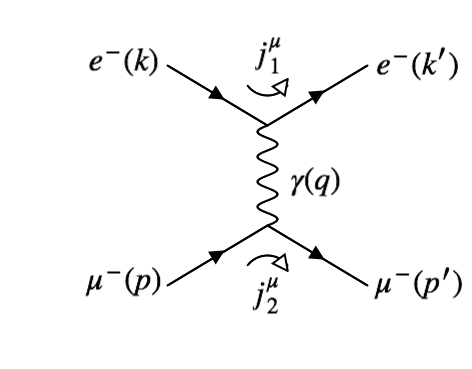
\includegraphics[width=0.5\textwidth]{images/web_feynman/image_87.png}
    \caption[Scattering of electrons and muons with momenta labels]{Scattering of electrons and muons with momenta labels.}
    \label{fig:ch8_EMuToEMuMomenta}
  \end{center}
\end{figure}

The transition amplitude is then:

\begin{eqnarray*}
  T_{fi} & = & -i\int j^{1}_{\mu}\left(\frac{-1}{q^2}\right)j^{\mu}_2 \mathrm{d}^4x \\
  & = & i\e\int\mathrm{d}^4x\bar{u}(k')\e^{ik'x}\gamma_{\mu}u(k)\e^{-ikx}\left(\frac{-1}{q^2}\right)\left(-\e\right)\bar{u}(p')e^{ip'x}\gamma^{\mu}u(p)\e^{-ipx} \\
  & = & \frac{i\e^2}{q^2}\int\mathrm{d}^4x\e^{i\left(k'+p'-k-p\right)}
        \Big[\bar{u}\left(k'\right)\gamma_{\mu}u\left(k\right)\Big]
        \Big[\bar{u}\left(p'\right)\gamma^{\mu}u\left(p\right)\Big]
\end{eqnarray*}

As before for $|T_{fi}|^2$, one exponential term becomes the phase-space factor and the second becomes the product of the volume and time.

\[
  |T_{fi}|^2 = \frac{\e^4}{q^4}
      \Big[\bar{u}\left(k'\right)\gamma_{\mu}u\left(k\right)\Big]
      \Big[\bar{u}\left(p'\right)\gamma^{\mu}u\left(p\right)\Big]
      \Big[\bar{u}\left(k'\right)\gamma_{\mu}u\left(k\right)\Big]^{\dagger}
      \Big[\bar{u}\left(p'\right)\gamma^{\mu}u\left(p\right)\Big]^{\dagger}
\]

The Hermitian conjugates are:

\begin{eqnarray*}
  \big(u^{\dagger}(p')\gamma^0\gamma^{\mu}u(p)\big)^{\dagger} & = & u^{\dagger}(p)\gamma^{\mu\dagger}\gamma^{0\dagger}u(p') \\
  & = & u^{\dagger}(p)\gamma^{\mu\dagger}\gamma^0u(p') \\
  & = & -u^{\dagger}(p)\gamma^{\mu}\gamma^0u(p') \\
  & = & u^{\dagger}(p)\gamma^0\gamma^{\mu}u(p') \\
  & = & \bar{u}(p)\gamma^{\mu}u(p')
\end{eqnarray*}

and similarly for the other term.

\[
  \Rightarrow |T_{fi}|^2 = \frac{\e^4}{q^4}
                           \Big[\bar{u}(k')\gamma_{\mu}u(k)\Big]
                           \Big[\bar{u}(k)\gamma_{\nu}u(k')\Big]
                           \Big[\bar{u}(p')\gamma^{\mu}u(p)\Big]
                           \Big[\bar{u}(p)\gamma^{\nu}u(p')\Big]
\]

\begin{eqnarray*}
  \Big[\bar{u}(k')\gamma_{\mu}u(k)\Big]
  \Big[\bar{u}(k)\gamma_{\nu}u(k')\Big]
  & \quad & \textrm{is the electron tensor} \\
  \Big[\bar{u}(p')\gamma_{\mu}u(p)\Big]
  \Big[\bar{u}(p)\gamma_{\nu}u(p')\Big]
  & \quad & \textrm{is the muon tensor}
\end{eqnarray*}

\[
  |T_{fi}|^2 = \frac{\e^4}{q^4} {}^{\e}L_{\mu\nu} {}^{\mu}L^{\mu\nu}
\]

In order to calculate the transition amplitude correctly the amplitude must be summed over all initial states, summed over all final spin states and averaged over all initial spin states:

\[
  ^{\e}L_{\mu\nu} = \frac{1}{2}\sum_{S}\sum_{S'} \bar{u}(k')\gamma_{\mu}u(k)\bar{u}(k)\gamma_{\nu}u(k')
\]

Writing this explicitly in terms of individual matrix elements, $\alpha$, $\beta$, $\gamma$, $\delta$:

\[
  ^{\e}L_{\mu\nu} = \frac{1}{2}\sum_{S}\sum_{S'}\bar{u}(k')_{\alpha}\gamma_{\mu}^{\alpha\beta}u(k)_{\beta}\bar{u}(k)_{\gamma}\gamma_{\nu}^{\gamma\delta}u(k')_{\delta}
\]

where the factor of $1/2$ is due to the averaging over initial spin states.

These values are all elements of tensors, so they can be reordered:

\begin{eqnarray*}
  ^{\e}L_{\mu\nu} & = & \frac{1}{2}\sum_{S}\sum_{S'}u(k')_{\delta}\bar{u}(k')_{\alpha} \left(\gamma_{\mu}^{\alpha\beta}\right)u(k)_{\beta}\bar{u}(k)_{\gamma}\gamma_{\nu}^{\gamma\delta} \\
  & = & \sum_{S}\sum_{S'}\left(\not{k}' + m\right)_{\delta\alpha} \left(\gamma_{\mu}^{\alpha\beta}\right) \left(\not{k} + m\right)_{\beta\gamma}
\end{eqnarray*}

So ${}^{\e}L_{\mu\nu}$ is reduced to the trace of the product of four $4 \times 4$ matrices:

\begin{eqnarray*}
  {}^{\e}L_{\mu\nu} & = & \frac{1}{2}Tr\Big[ \left(\not{k}' + m\right)\left(\gamma_{\mu}\right)\left(\not{k} + m\right)\left(\gamma_{\nu}\right) \Big] \\
  {}_{\mu}L_{\mu\nu} & = & \frac{1}{2}Tr\Big[ \left(\not{p}' + m\right)\left(\gamma_{\mu}\right)\left(\not{p} + m\right)\left(\gamma_{\nu}\right) \Big]
\end{eqnarray*}

Denoting the electron mass by $m$ and the muon mass by $M$ gives:

\begin{eqnarray*}
  |T_{fi}|^2 & = & \frac{\e^4}{q^4}\frac{1}{2}Tr\Big[\left(\not{k}' + m\right)\gamma_{\mu}\left(\not{k} + m\right)\gamma_{\nu}\Big]\frac{1}{2}Tr\Big[\left(\not{p}' + M\right)\gamma^{\mu}\left(\not{p} + M\right)\gamma^{\nu}\Big] \\
  & = & \frac{\e^4}{4q^4}Tr\Big[\left(\not{k}' + m\right)\gamma_{\mu}\left(\not{k}+m\right)\gamma_{\nu}\Big] Tr\Big[\left(\not{p}' + M\right)\gamma^{\mu}\left(\not{p} + M\right)\gamma^{\nu} \Big]
\end{eqnarray*}

The only non-zero terms are terms involving two or four $\gamma$ matrices.  eg $\left(\not{k}'\gamma_{\mu}m\gamma_{\nu}\right) = 0$.

\begin{eqnarray*}
  \textrm{So } |T_{fi}|^2 & = & \frac{\e^4}{4q^4} Tr[\gamma_{\delta}\gamma_{\mu}\gamma_{\sigma}\gamma_{\nu}k'^{\delta}k^{\sigma} + \gamma_{\mu}\gamma_{\nu}m^2]Tr[\gamma^{\delta}\gamma^{\mu}\gamma^{\sigma}\gamma^{\nu}p'_{\delta}p_{\sigma} + \gamma^{\mu}\gamma^{\nu}M^2] \\
  & = & \frac{\e^4}{q^4} \left( \left(g_{\delta\nu}g_{\nu\sigma} - g_{\delta\sigma}g_{\nu\mu} + g_{\delta\mu}g_{\sigma\nu}\right)k'^{\delta}k^{\sigma} + g^{\mu_\nu}m^2\right) \\
      && \times 4 \left( \left(g^{\delta\nu}g^{\nu\sigma} - g^{\delta\sigma}g^{\nu\mu} + g^{\delta\mu}g^{\sigma\nu}\right)p'_{\delta}p_{\sigma} + g_{\mu\nu}M^2\right) \\
  &&\textrm{Multiplying out: }\\
  |T_{fi}|^2 & = & \frac{8\e^4}{q^4}\left( \left(k'\cdot p'\right)\left(k\cdot p\right) + \left(k'\cdot p\right)\left(k\cdot p'\right) - m^2\left(p'\cdot p\right) - M^2\left(k'\cdot k\right) + m^2M^2\right)
\end{eqnarray*}

In the relativistic limit the $m^2$ and $M^2$ terms can be neglected.

\[
  \Rightarrow |T_{fi}|^2 = \frac{8\e^4}{q^4}\left(\left(k'\cdot p'\right)\left(k\cdot p\right) + \left(k'\cdot p\right)\left(k\cdot p\right)\right)
\]

Expressing this in terms of the Mandelstran variables gives:

\begin{eqnarray*}
  s   & =    & \left(k + p\right)^2 \\
      & \sim & 2k\cdot p \\
      & \sim & 2k'\cdot p' \\
  q^2 & =    & t \\
      & =    & \left(k - k'\right)^2 \\
      & =    & \left(p - p'\right)^2 \\
      & \sim & -2k\cdot k' \\
      & \sim &  2p\cdot p' \\
  u   & =    & \left(k - p'\right)^2 \\
      & \sim & -2p'\cdot k \\
      & \sim & -2k'\cdot p \\
  \textrm{So } |T_{fi}|^2 & = & \frac{8\e^4}{t^2}\left(\frac{s}{2}\frac{s}{2} + \left(\frac{-u}{2}\right)\left(\frac{-u}{2}\right)\right) \\
  & = & \frac{2\e^4}{t^2}\left(s^2 + u^2\right) \\
  & = & 2\e^4\left(\frac{s^2 + u^2}{t^2}\right) \\
  \Rightarrow \frac{\mathrm{d}\sigma}{\mathrm{d}\Omega} & = & \frac{1}{64\pi^2s}|T_{fi}|^2 \\
  & = & \frac{\e^4}{32\pi^2s}\left(\frac{s^2 + u^2}{t^2}\right)
\end{eqnarray*}

\section{Cross section for \texorpdfstring{$\e^+\e^- \to \mu^+\mu^-$}{EEToMuMu}}

This cross section can be easily derived from $e \mu \to e \mu$ scattering.  Compare the Feynmann diagrams shown in figure \ref{fig:ch8_EMuToEMuMomenta}.

\begin{figure}[!htb]
  \begin{center}
    \begin{tabular}{cc}
      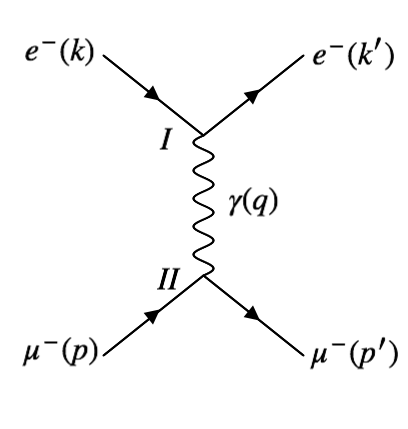
\includegraphics[width=0.4\textwidth]{images/web_feynman/image_25.png} &
      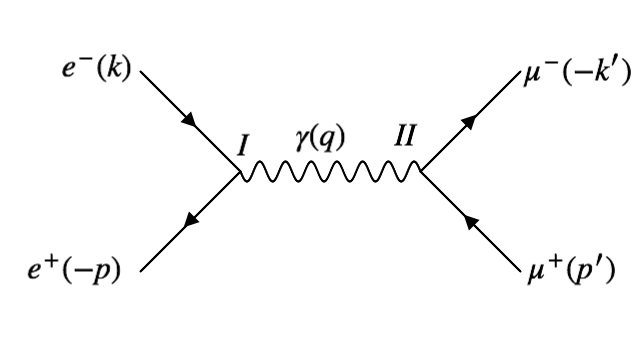
\includegraphics[width=0.6\textwidth]{images/web_feynman/image_26.png}
    \end{tabular}
    \caption[Scattering of electrons and muons with momenta in the $s$ and $t$ channels]{Scattering of electrons and muons with momenta in the $s$ and $t$ channels.}
    \label{fig:ch8_EMuToEMuMomentaSTChannels}
  \end{center}
\end{figure}

Comparing the vertices:

\[
\begin{array}{ccc}
  \textrm{For }I  & k \to k'  & \textrm{in } e\mu \to e\mu         \\
                  & k \to -p  & \textrm{in } e^+e^- \to \mu^+\mu^- \\
  \textrm{For }II & p \to p'  & \textrm{in } e\mu \to e\mu         \\
                  & -k'\to p' & \textrm{in } e^+e^- \to \mu^+\mu^-
\end{array}
\]

So between the two processes there is an interchange of $k'$ with $-p$ and $p$ with $-k'$.

Recall for $e^-\mu^-$ scattering:

\begin{eqnarray*}
  |T_{fi}|^2 & = & \frac{8\e^4}{q^4}\left(\left(k'\cdot p'\right)\left(k\cdot p\right) + \left(k'\cdot p\right)\left(k\cdot p'\right)\right) \\
  \textrm{and } q^4 & = & 4\left(k\cdot k\right)^2 \\
\end{eqnarray*}

So $|T_{fi}|^2$ for $e^+e^-$ is:

\begin{eqnarray*}
  |T_{fi}|^2 & = & \frac{8\e^4}{4\left(k\cdot p\right)^2}\left(\left(p\cdot p'\right)\left(k\cdot k'\right) + \left(p\cdot k'\right)\left(k\cdot p\right)\right) \\
  & = & \frac{2\e^4}{\left(k\cdot p\right)^2}\left(\left(p\cdot p'\right)\left(k\cdot k'\right) + \left(p\cdot k'\right)\left(k\cdot p'\right)\right) \\
  & = & \frac{2\e^4}{\left(\frac{s}{2}\right)^2}\left(\left(\frac{-t}{2}\right)\left(\frac{-t}{2}\right) + \left(\frac{-u}{2}\right)\left(\frac{-u}{2}\right)\right) \\
  \Rightarrow |T_{fi}|^2_{e^+e^-} & = & 2\e^4\left(\frac{t^2 + u^2}{s^2}\right) \\
  \Rightarrow \frac{\mathrm{d}\sigma}{\mathrm{d}\Omega}_{e^+e^-} & = & \frac{1}{64\pi^2}\times2\e^4\left(\frac{t^2 + u^2}{s^2}\right) \\
  & = & \frac{\e^4}{32\pi^2}\left(\frac{t^2 + u^2}{s^2}\right)
\end{eqnarray*}

In comparison with $e\mu \to e\mu$, the values of $s$ and $t$ are simply interchanged.

\subsection{Total cross-section}

To find the total cross-section, integrate with respect to $\Omega$ and evaluate $s$, $t$ and $u$ in terms of the energy and angle of scattering in the centre of mass frame:

\begin{eqnarray*}
  s   & \sim & 2k\cdot p \\
      & =    & 4E_{e^-}E_{e^+} \\
  t^2 & =    & 4\left(k\cdot k'\right)^2 \\
      & =    & 4\left(E_{e^-}E_{\mu^+} - p_{e^-}\cdot p_{\mu^+} \right)^2 \\
      & =    & 4E_{e^-}E_{\mu^+}\left(1 - \cos\theta\right)^2 \\
  u^2 & =    & 4\left(k\cdot p'\right)^2 \\
      & =    & 4E_{e^-}E_{\mu^-}\left(1 + \cos\theta\right)^2 \\
  \Rightarrow \frac{\mathrm{d}\sigma}{\mathrm{d}\Omega} & = & \frac{1}{64\pi^2s}2\e^4\frac{4\left(E_{e^-}E_{\mu^+}\left(1 - \cos\theta\right)^2 + E_{e^-}E_{\mu^-}\left(1 + \cos\theta\right)^2\right)}{16 E_{e^+}E_{e^-}}
\end{eqnarray*}

But in the centre of mass system:

\[
  E_{e^-} = E_{e^+} = E_{\mu^-} = E_{\mu^+}
\]

\begin{eqnarray*}
  \Rightarrow \frac{\mathrm{d}\sigma}{\mathrm{d}\Omega} & = & \frac{1}{64\pi^2s}\e^4\left(1 + \cos\theta\right)^2 \\
  \sigma & = & \int_{-\pi}^{\pi}\frac{\mathrm{d}\sigma}{\mathrm{d}\Omega}\mathrm{d}\Omega \\
  \mathrm{d}\Omega & = & 2\pi \mathrm{d}\left(\cos\theta\right) \\
  \alpha & = & \frac{\e^2}{4\pi} \\
  \Rightarrow \sigma & = & \int_0^{\pi}\frac{\alpha^2}{4s}\left(1 + \cos^2\theta\right) 2\pi\mathrm{d}\left(\cos\theta\right) \\
  & = & \frac{2\pi\alpha^2}{4s}\int_{1}^{-1}\left(1 + x^2\right)\mathrm{d}x \\
  \left(\textrm{as } x \right.& = &\left. \cos\theta\right) \\
  & = & \frac{2\pi\alpha^2}{4s}\Big[-\cos\theta - \frac{1}{3}\cos^3\theta\Big]_0^{\pi} \\
  & = & \frac{4\pi\alpha^2}{3s}
\end{eqnarray*}

The annihilation process falls off as a function of $1/s$.  Had it not been for $q\bar{q}$ resonances, eg $Z^0$, particle physics would have become rather uninteresting.

Note that using similar methods it is possible to calculate Bhabha scattering:

\begin{figure}[!htb]
  \begin{center}
    \begin{tabular}{cc}
      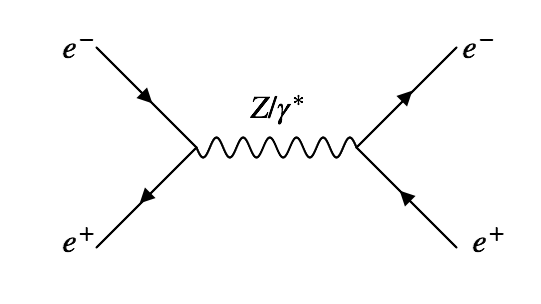
\includegraphics[width=0.5\textwidth]{images/web_feynman/image_28.png} &
      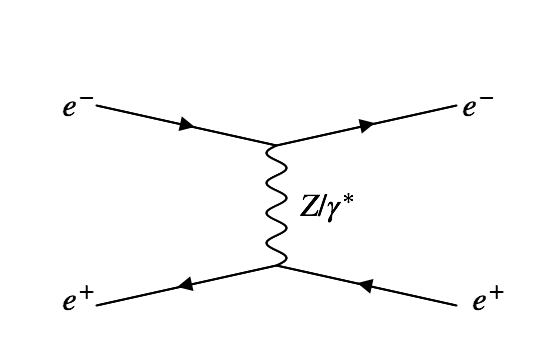
\includegraphics[width=0.5\textwidth]{images/web_feynman/image_29.png}
    \end{tabular}
    \caption[Lowest order Bhabha scattering processes]{Lowest order Bhabha scattering processes.}
    \label{fig:ch8_Bhabha}
  \end{center}
\end{figure}

There are higher order interactions which have not been taken into account, such as:

\begin{figure}[!htb]
  \begin{center}
    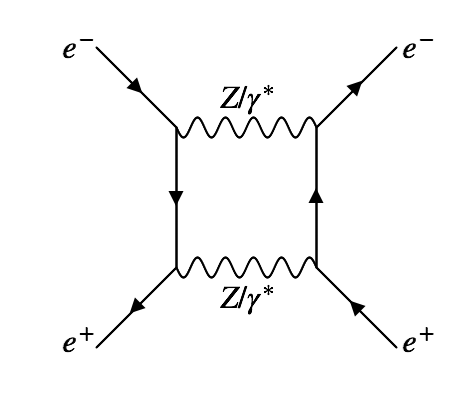
\includegraphics[width=0.5\textwidth]{images/web_feynman/image_30.png}
    \caption[Higher order Bhabha scattering processes]{Higher order Bhabha scattering processes.}
    \label{fig:ch8_Bhabha2}
  \end{center}
\end{figure}

\section{The ratio \texorpdfstring{$R$ at $\e^+\e^-$}{RAtEE} colliders}

\[
  R = \frac{\sigma(e^+e^- \to hadrons)}{\sigma(e^+e^- \to \mu^+\mu^-)}
\]

At low energies $e^+e^-$ can annihilate into systems containing $u$ or $d$ quarks with quarks subsequently hadronising.  They can annihilate through the virtual photon to make $q\bar{q}$ resonances such as the $\rho(770)$.  As the energy increases $s\bar{s}$, $c\bar{c}$ and $b\bar{b}$ states can be formed.  At very high energies $t\bar{t}$ states can be formed, although such $e^+e^-$ colliders have yet to be built.

Consider the contribution to $R$ from on generation of $q\bar{q}$ pairs:

\begin{eqnarray*}
  R & = & \frac{\left(\left(\frac{2}{3}\right)^2 + \left(\frac{-1}{3}\right)^2\right)\times\e^2\times 3}{\e^2} \\
  & = & \frac{15}{9} \textrm{ per generation}
\end{eqnarray*}

By the time the energy is $\sqrt{s}>2m_b$, $R$ should be be $\sim \frac{11}{3}$.

\diagram

Superimposed are the resonances, such as the $J/\psi$ and $\Upsilon$ family.  There are resonances at $\rho(770)$, $J/\psi(3088)$ and $\Upsilon(10588)$.  At Babar, the $e^+e^-$ collider runs at the $\Upsilon(4S)$ resonances, which decays almost exclusively to $b\bar{b}$ pairs.

\begin{figure}[!htb]
  \begin{center}
    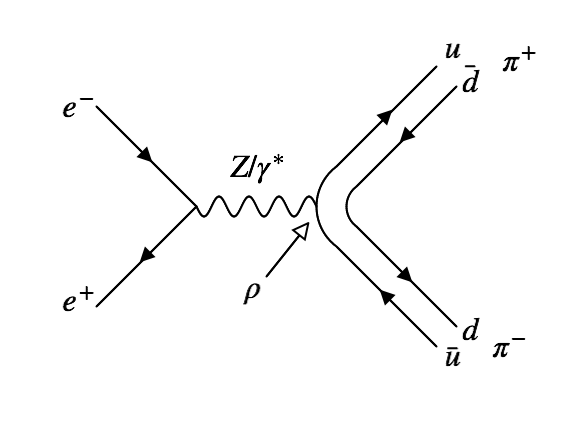
\includegraphics[width=0.5\textwidth]{images/web_feynman/image_31.png}
    \caption[Hadron production ($e^+e^-\to\pi\pi$)]{Hadron production, ($e^+e^-\to\pi\pi$), with a resonant contribution.}
    \label{fig:ch8_EpEmToPiPi}
  \end{center}
\end{figure}

Although the simple model predicting $\frac{11}{3}$ for $R$ for $\sqrt{s}>2m_b$ gives a reasonable description of the data, this is not the complete picture.  The actual value is somewhat higher due to gluon radiation in the final state of the hadronic system:

\begin{figure}[!htb]
  \begin{center}
    \includegraphics[width=0.5\textwidth]{images/web_feynman/image_32.png}
    \caption[Hadron production with gluon radiation]{Hadron production with gluon radiation.}
    \label{fig:ch8_EpEmToQQG}
  \end{center}
\end{figure}

So there is a higher order correction to $R\sim\frac{11}{3}$.

\begin{figure}[!htb]
  \begin{center}
    \includegraphics[width=0.5\textwidth]{images/web_feynman/image_34.png}
    \caption[Hadron production and $R$ for $\sqrt{s}>2m_b$]{Hadron production and $R$ for $\sqrt{s}>2m_b$.}
    \label{fig:ch8_EpEmR}
  \end{center}
\end{figure}

At the $Z^0$ mass resonance, an analogous quantity is the ratio of the partial decay widths:

\[
  R_Z = \frac{\Gamma(Z^0 \to hadrons)}{\Gamma(Z^0 \to \mu^+ \mu^-)}
\]

To lowest order, $R_Z = 20.09$, however the measured value is $20.79 \pm 0.04$.  This $3.5\%$ discrepency is due entirely to higher order QCD corrections and gives a good way to measure $\alpha_s$.

\section{Helicity conservation at high energies}

It is possible to gain further insight into cross-section calculations and their angular distributions by looking at the helicity of particles.  The states are:

\begin{eqnarray*}
  U_L & = & \frac{1}{2}\left(1 - \gamma^5\right)u \\
  U_R & = & \frac{1}{2}\left(1 + \gamma^5\right)u \\
  \bar{U}_L & = & U_L^{\dagger}\gamma^0 \\
  & = & \frac{1}{2}\left(U^{\dagger}\right)\left(1 - \gamma^5\right)^{\dagger}\gamma^0 \\
  & = & \frac{1}{2}U^{\dagger}\left(1 - \gamma^5\right)\gamma^0 \\
  & = & \frac{1}{2}U^{\dagger}\gamma^0\left(1 + \gamma^5\right) \\
  & = & \frac{1}{2}\bar{U}\left(1 + \gamma^5\right)
\end{eqnarray*}

At high energies the electromagnetic interaction conserves helicity.

Consider the electromagnetic current:

\begin{eqnarray*}
  \bar{u}\gamma^{\mu}u & = & \left(\bar{U}_L + \bar{U}_R\right)\gamma^{\mu}\left(U_L + U_R\right) \\
  \bar{U}_L\gamma^{\mu}U_R & = & \frac{1}{2}\bar{u}\left(1 + \gamma^5\right)\gamma^{\mu}\frac{1}{2}\left(1 + \gamma^5\right)u \\
  & = & \frac{1}{4}\bar{u}\gamma^{\mu}\left(1 - \gamma^5\right)\left(1 + \gamma^5\right)u \\
  & = & \frac{1}{4}\bar{u}\gamma^{\mu}\left(1 - \left(\gamma^5\right)^2\right)u \\
  & = & 0
\end{eqnarray*}

Helicity conservation requires that the incoming electron and positron have opposite helicities, as do the outgoing muons.

In the centre of mass system:

\begin{figure}[!htb]
  \begin{center}
    \includegraphics[width=0.75\textwidth]{images/web_feynman/image_33.png}
    \caption[Helicity conservation in a centre of mass system]{Helicity conservation in a centre of mass system.}
    \label{fig:ch8_helicityConservation}
  \end{center}
\end{figure}

The reaction proceeds via a photon of spin$-1$ so the amplitudes are proportional to the rotation matrices:

\[
  d^j_{\lambda\lambda'}(\theta) = \langle j\lambda'|e^{-i\theta J_y}|j \lambda\rangle
\]

where $y$ is perpendicular to the reaction plane.  The rotation matrices can be calculated using angular momentum theory.

\[
  \begin{array}{ccccccc}
  d^1_{1,1}  (\theta) & = & d^1_{-1,-1}(\theta) & = & \frac{1}{2}\left(1 + \cos\theta\right) & \sim & -\frac{u}{s} \\
  d^1_{1,-1} (\theta) & = & d^1_{-1,1} (\theta) & = & \frac{1}{2}\left(1 - \cos\theta\right) & \sim & -\frac{t}{s}
  \end{array}
\]

Squaring and adding the above:

\[
  \frac{\mathrm{d}\sigma}{\mathrm{d}\Omega} \propto \frac{t^2 + u^2}{s^2}
\]

\cleardoublepage
\chapter{Massless spin\texorpdfstring{$-1$}{1} particles (photons)}
\chaptermark{Massless spin\texorpdfstring{$-1$}{-1} particles}

\section{Maxwell's equations and the definition of classical potentials}

\[
  \begin{array}{ccccc}
  I   & \quad & \Div{E}  & = & \rho \\
  II  &       & \Div{B}  & = & 0 \\
  III &       & \Curl{E} & = & -\ul{\dot{B}} \\
  IV  &       & \Curl{B} & = & \ul{J} + \ul{\dot{E}}
  \end{array}
\]

The potentials are defined as:

\begin{eqnarray*}
  \ul{B} & = & \Curl{A} \\
  \Curl{E} & = & -\frac{\partial \Curl{A}}{\partial t} \\
  & = & -\ul{\nabla}\times{\left(\frac{\partial \ul{A}}{\partial t}\right)} \\
  \textrm{So } \ul{\nabla}\times{\left(\ul{E} + \frac{\partial\ul{A}}{\partial t}\right)} & = & \ul{0}
\end{eqnarray*}

The solution is:

\[
  \ul{E} + \frac{\partial \ul{A}}{\partial t} = -\Grad{\phi}
\]

as the gradient of a scalar function has zero curl everywhere.

$I$ and $IV$ give:

\begin{eqnarray}
  \Div{E} & = & \rho \nonumber \\
  \ul{E}  & = & -\Grad{\phi} - \frac{\partial \ul{A}}{\partial t} \nonumber \\
  \Rightarrow -\nabla^2\phi - \frac{\partial}{\partial t}\left(\Div{A}\right) & = & \rho \nonumber \\
  \textrm{So } \nabla^2\phi - \frac{\partial^2\phi}{\partial t^2} + \frac{\partial^2\phi}{\partial t^2} + \frac{\partial}{\partial t}\Div{A} & = & \rho \label{eq:maxwell1} \\
  \Curl{B} & = & \ul{J} + \frac{\partial \ul{E}}{\partial t} \nonumber \\
  \ul{\nabla}\times\Curl{A} & = & \ul{J} + \frac{\partial \ul{E}}{\partial t} \nonumber \\
  & = & \ul{J} + \frac{\partial}{\partial t}\left(-\Grad{\phi} - \frac{\partial \ul{A}}{\partial t}\right) \nonumber \\
  & = & \ul{J} - \Grad{\frac{\partial\phi}{\partial t}} - \frac{\partial^2\ul{A}}{\partial t^2} \nonumber \\
  \textrm{or } \Grad{\left(\Div{A}\right)} - \nabla^2\ul{A} & = & \ul{J} - \Grad{\frac{\partial \phi}{\partial t}} - \frac{\partial^2 \ul{A}}{\partial t^2} \nonumber \\
  \Rightarrow \nabla^2\ul{A} - \frac{\partial^2\ul{A}}{\partial t^2} - \Grad{\left(\Div{A}\right)} - \frac{\partial}{\partial t}\Grad{\phi} & = & \ul{J} \label{eq:maxwell2} \\
\end{eqnarray}

Equations (\ref{eq:maxwell1}) and (\ref{eq:maxwell2}) can be written as:

\begin{eqnarray*}
  \Box^2A^{\mu} - \partial^{\mu}\partial_{\nu}A^{\nu} & = & J^{\mu} \\
  \textrm{where } \Box^2 & = & \left(\frac{\partial^2}{\partial t^2},-\nabla^2\right) \\
  A^{\mu} & = & \left(\phi,\ul{A}\right) \\
  J^{\mu} & = & \left(\rho,\ul{J}\right)
\end{eqnarray*}

Therefore the electromagnetic field is given by the four-potential $A^{\mu}$ which satisfies the above equation.  For a free electromagnetic field $\left(\rho,\ul{J}\right) = 0$.

Consider the polarisation states for a free photon.  Since there is a four-potential there appears to be four polarisation states.  These states reduce to the well known two polarisations states of the free photon.  The four states for a photon travelling in the $z-$direction are:

\begin{eqnarray*}
  |1,0,0,0\rangle & \quad & \textrm{time-like polarisation} \\
  |0,1,0,0\rangle & \quad & \textrm{polarisation in the $x$ direction} \\
  |0,0,1,0\rangle & \quad & \textrm{polarisation in the $y$ direction} \\
  |0,0,0,1\rangle & \quad & \textrm{polarisation in the $z$ direction} \\
\end{eqnarray*}

For virtual photons all four polarisation states exist, whereas for real photons only tranverse polarisation states exist.

Applying the Lorentz condition:

\begin{eqnarray*}
  \partial_{\mu}A^{\mu} & = & 0 \\
  \Box^2A^{\mu} & = & J^{\mu}
\end{eqnarray*}

This makes the time-like component depend on the spatial components so that the time-like component is no longer independent.  For free photons $J^{\mu} = 0^{\mu}$, so $\Box^2A^{\mu} = 0^{\mu}$ and the solutions are plane waves:

\[
  A^{\mu} = \epsilon_i^{\mu}\e^{-iqx}
\]

where $\epsilon_i$ are the four polarisation states.

The Lorentz condition gives:

\begin{eqnarray*}
  \partial_{\mu}A^{\mu} & = & \partial_{\mu}\epsilon_i^{\mu}\e^{q_{\mu}x^{\mu}} \\
  & = & 0 \\
  \Rightarrow -iq_{\mu}\epsilon_i^{\mu}\e^{-q_{\mu}x^{\mu}} & = & 0
\end{eqnarray*}

So the Lorentz condition reduces to:

\begin{eqnarray*}
  q_{\mu}\epsilon_i^{\mu} & = & 0 \\
  \Rightarrow q_0\epsilon_i^0 & = & q_k\epsilon_i^k
\end{eqnarray*}

So the time-like component is dependent on the space-like components.  To reduce to two polarisation vector a gauge transformation is applied.  Recall that $\ul{E}$ and $\ul{B}$ in classic electromagnetism come from the field tensor:

\[
  F^{\mu\nu} = \partial^{\mu}A^{\nu} - \partial^{\nu}A^{\mu}
\]

$F^{\mu\nu}$ is unchanged and this $\ul{E}$ and $\ul{B}$ are unchanged under the gauge transformation:

\[
  A'^{\mu} \to A^{\mu} + \partial^{\mu}\Lambda
\]

where $\Lambda$ is a scalar field.  $\Lambda$ satisfies the Lorentz condition.

\begin{eqnarray*}
  \textrm{Let } \Lambda & = & ia\e^{-iq_{\mu}x^{\mu}} \\
  \partial_{\mu}\partial^{\mu}\Lambda & = & \left(-iq_{\mu}\right)\left(-iq^{\mu}\right)ia\e^{-iq_{\mu}x^{\mu}} \\
  & = & -iaq^2\e^{-iqx}
\end{eqnarray*}

But $q^2 = E^2 - p^2$ and is equal to zero for a real photon, so $\partial^{\mu}_{\mu} = 0$ and the Lorentz condition is satisfied.  Substituting $\Lambda$ and $A^{\mu} = \epsilon^{\mu}\e^{iq_{\mu}x^{\mu}}$ into the gauge tranformation gives:

\begin{eqnarray*}
  A'^{\mu} & \to & \epsilon^{\mu}\e^{-iqx} + \left(-iq^{\mu}\right)ia\e^{-iqx} \\
  & = & \epsilon^{\mu}\e^{-iqx} + aq^{\mu}\e^{-iqx}
\end{eqnarray*}

So the gauge transformation simplifies to:

\[
  \epsilon'^{\mu} \to \epsilon^{\mu} + aq^{\mu}
\]

So two polarisation vectors $\epsilon$ and $\epsilon'^{\mu}$ which differ by a multiple of $q^{\mu}$, describe the same photon.  This means the time component must be zero.  $\epsilon_0 = 0$.

So the Lorentz condition reduces to $\ul{\epsilon}\cdot\ul{q} = 0$.  From this only two independent polarisation vectors can exist and they must be perpendicular to $\ul{q}$.  So the states are:

\begin{eqnarray*}
  \ul{\epsilon}_1 & = & \left(1,0,0\right) \\
  \ul{\epsilon}_2 & = & \left(0,1,0\right)
\end{eqnarray*}

They can also be expressed as circular polarisation:

\begin{eqnarray*}
  \ul{\epsilon}_R & = & \frac{1}{\sqrt{2}}\left(\ul{\epsilon}_1 + i\ul{\epsilon}_2\right) \\
  \ul{\epsilon}_L & = & \frac{1}{\sqrt{2}}\left(\ul{\epsilon}_1 - i\ul{\epsilon}_2\right)
\end{eqnarray*}

\subsection{Virtual photons and the photon propagator}

For virtual photons, by imposing the Lorentz condition:

\begin{eqnarray*}
  \Box^2A^{\mu} & = & J^{\mu} \\
  & = & g^{\mu\nu}J_{\nu} \\
  \textrm{By inspection: } A^{\mu} & = & -\frac{g^{\mu\nu}}{q^2}J_{\nu}
\end{eqnarray*}

The solution can be derived by the propagator approach:

\begin{equation}
  A^{\mu}(x') = \int G(x';x)j^{\mu}(x)\mathrm{d}^4x \label{eq:propagator}
\end{equation}

From the Lorentz condition:

\begin{eqnarray*}
  \Box^2A^{\mu}(x') & = & j^{\mu}(x') \\
  & = & \int\mathrm{d}^4x \delta^4(x'-x)j^{\mu}(x) \\
  \textrm{Also from (\ref{eq:propagator}):} \Box^2A^{\mu}(x') & = & \int\Box^2G(x',x)j^{\mu}(x)\mathrm{d}^4x
\end{eqnarray*}

Comparing the expressions for $\Box^2A^{\mu}(x')$:

\[
  \Box^2G(x',x) = \delta^4(x' - x)
\]

Translating into four-momentum space via a Fourier transform:

\begin{eqnarray*}
  \frac{1}{\left(2\pi\right)^4} \int\mathrm{d}^4q\left(-iq\right)^2G(q)\e^{-iq\left(x - x'\right)} & = & \frac{1}{\left(2\pi\right)^4}\int\mathrm{d}^4q \e^{-iq\left(x' - x\right)} \\
  \Rightarrow G(q) & = & -\frac{1}{q^2} \\
  \textrm{So } A^{\mu}(x) & = & -\frac{j^{\mu}(x)}{q^2} \\
  & = & -\frac{-g^{\mu\nu}j_{\nu}(x)}{q^2}
\end{eqnarray*}

When considering the propagator approach theory it is found that the propagator in four-momentum space is the inverse of the equation describing the free propagation of virtual particles.  In four-momentum space the propagator for a Klein-Gordon particle is obtained by inverting the Klein-Gordon equation, multiplied by $i$.

\[
  i\left(\Box^2 + m^2\right)\phi = -iV\phi
\]

So the Klein-Gordon propagator is:

\begin{eqnarray*}
  \frac{1}{i\left(\Box^2 + m^2\right)} & = & \frac{-i}{\Box^2 + m^2} \\
  \Box^2 & = & \partial_{\mu}\partial^{\mu} \\
  & = & \frac{i\partial_{\mu}i\partial^{\mu}}{i^2} \\
  & = & -p^{\mu}p_{\mu} \\
  & = & -p^2
\end{eqnarray*}

So the propagator is $\displaystyle\frac{i}{p^2 - m^2}$.

Consider the Dirac equation:

\[
  \Big[\left(\alpha p + \beta m\right) + \e\left(\alpha A - A^0I\right)\Big] \psi = E\psi
\]

where the Dirac potential is $\alpha A - A^0I$.

Converting this equation to convariant form by premultiplying by $\beta$ gives:

\[
  \Big[\beta\alpha p + \beta^2m + \e\left(\beta\alpha A - \beta A^0I\right)\Big]\psi = \beta E\psi
\]

Rearranging:

\begin{eqnarray*}
  \left(\beta E - \beta \alpha p - \beta^2 m\right)\psi & = & \e\left( \beta\alpha A - \beta A^0\right)\psi \\
  \left(\gamma^0 E - \gamma^kp_k -Im\right)\psi & = & -\e\left(\beta A^0 - \beta\alpha A\right)\psi \\
  \left(\not{p} - m \right)\psi & = & -\e\not{A}\psi \\
  \Rightarrow -i\left(\not{p} - m\right)\psi & = & i\e\not{A}\psi \\
  & = & -iV\psi
\end{eqnarray*}

So the propagator is:

\begin{eqnarray*}
  \frac{1}{-i\left(\not{p} - m\right)} & = & \frac{i\left(\not{p} + m\right)}{\left(\not{p}-m\right)\left(\not{p} + m\right)} \\
  & = & \frac{i\left(\not{p} + m\right)}{\not{p}^2 - m^2} \\
  & = & \frac{i\left(\not{p} + m\right)}{p^2 - m^2} \\
  & = & \frac{i\sum_{spins}u\bar{u}}{p^2 - m^2} \textrm{via the completeness relation}
\end{eqnarray*}

This is the general form of the propagator of a virtual particle where the sum is over eg all spin states of the electron or polarisation states of the photon.

\subsection{Real and virtual photons and the significance of longitudinal and time-like polarisations}

Consdier a typical process involving photon exchange ie the photon is sandwiched between two currents:

\begin{eqnarray*}
  j^A_{\mu}(x)\left(\frac{-g^{\mu\nu}}{q^2}\right)j^B_{\nu}(x) & = & -j^A_{\mu}(x)\frac{1}{q^2}j^{B\mu}(x) \\
  & = & \frac{1}{q^2}\Big[j^A_1(x)j^{1B}(x) + j^A_2(x)j^{2B}(x) + j^A_3(x)j^{3B}(x) - j^A_0(x)j^{0B}(x) \Big]
\end{eqnarray*}

However, electromagnetic current is conserved:

\[
  \partial_{\mu}j^{\mu} = 0 \Rightarrow q_{\mu}j^{\mu} = 0
\]

\paragraph*{Proof} Consider $j^{\mu} = \bar{u}_f\e^{ip_fx}\gamma^{\mu}u_i\e^{-ip_ix}$.  Then if $q$ is the momentum of the exchanged photon and $q = p_f - p_i$ then:

\[
  \partial_{\mu}j^{\mu} \propto i\left(p_f - p_i\right)
\]

Therefore if $\partial_{\mu}j^{\mu} = 0$ then $q_{\mu}j^{\mu} = 0$.

Since $q$ can be taken to be parallel to the $x^3$ axis without loss of generality:

\[
  q_3j^1 = q_3j^2 = 0
\]

Applying the condition $q_{\mu}j^{\mu} = 0$ to the longitudinal and time-like components:

\begin{eqnarray*}
  q_{\mu}j^{\mu} & = & q_0j^0 - q_3j^3 \\
  \Rightarrow j^3 & =& \frac{q_0j^0}{q_3}
\end{eqnarray*}

Substituting this back into the amplitude:

\begin{eqnarray*}
  \frac{1}{q_3^2q^2}q_0^2j^A_0j^{0B} - \frac{1}{q^2}j^A_0j^{0B} & = & \frac{1}{q^2}j^A_0(x)j^{0B}(x)\left(\frac{q_0^2 - q_3^2}{q_3^2}\right) \\
  \textrm{but } q^2 & = & q_0^2 - q_3^2 \\
  \textrm{so } amplitude & = & \frac{j_0^A(x)j^{0B}(x)}{q_3^2}
\end{eqnarray*}

which is Coulomb's law in three-momentum space.

The completeness relation for real photons is:

\[
  \left(
    \begin{array}{c}
    1 \\
    0
    \end{array}
  \right)
  \left(1 0\right)
  +
  \left(
    \begin{array}{c}
    0 \\
    1
    \end{array}
  \right)
  \left(0 1\right)
  =
  \left(
    \begin{array}{cc}
    1 & 0 \\
    0 & 1
    \end{array}
  \right)
\]

However the same completeness relation can be used as for virtual photons.

\[
  \textrm{ie} -g^{\mu\nu} = 
  \left(
    \begin{array}{cccccc}
    -1 & & 0 & 0 & & 0 \\
      \begin{array}{c}
      0 \\
      0
      \end{array}
    &
    \Bigg\{
    &
      \begin{array}{c}
      1 \\
      0
      \end{array}
    &
      \begin{array}{c}
      0 \\
      1
      \end{array}
    &
    \Bigg\}
    &
      \begin{array}{c}
      0 \\
      0
      \end{array}
    \\
    0 & & 0 & 0 & & 1
    \end{array}
  \right)
\]

where the $\{ \cdots \}$ denotes the real parts of the polarisation.

The generalised form of virtual photons ($-g^{\mu\nu}$) is used for the completeness relation for virtual photons.

\cleardoublepage
% Copyright Aidan Randle-Conde 2007-2014
% http://www.aidansean.com/phd_notes
% Anyone is free to download, redistribute, edit and use these notes and the source tex files with the following restrictions:
% This 
%  This message is included in the tex source files.
%  Aidan Randle-Conde is credited as the author.
%  Images are correctly credited to their respective authors, as outlined in the references.
%  No part of these notes may be used for commercial purposes.

\chapter{Massive spin\texorpdfstring{$-1$}{1} particles}

For a massless photon the four-potential satisfies:

\[
  \Box^2A^{\mu} - \partial^{\mu}\partial_{\nu}A^{\nu} = j^{\mu}
\]

For a free particle $j^{\mu} = 0$

\begin{eqnarray*}
  \textrm{so }\Box^2A^{\mu} = \partial^{\mu}\partial_{\nu} & = & 0 \\
  \left( \frac{\partial^2}{\partial t^2}\right)A^{\mu} - \partial^{\mu}\partial_{\nu}A^{\nu} & = & 0 \\
  \left(E^2 + p^2\right)A^{\mu} - \partial^{\mu}\partial_{\nu}A^{\nu} & = & 0
\end{eqnarray*}

For masssive particles $E^2 = p^2 + m^2$, so a massive particle satisfies:

\[
  \Box^2A^{\mu} + m^2A^{\mu}-\partial^{\mu}\partial_{\nu} A^{\nu} = 
  \left\{
    \begin{array}{cc}
    0 & \quad\textrm{real} \\
    j^{\mu} & \quad\textrm{virtual}
    \end{array}
  \right.
\]

This the Proca equation.  Differentiating with respect to $\partial_{\mu}$:

\begin{eqnarray*}
  \partial_{\mu}\Box^2A^{\mu} + m^2\partial_{\mu}A^{\mu} - \partial_{\mu}\partial^{\mu}\partial_{\nu}A^{\nu} & = & \partial_{\mu}j^{\mu} \\
  & = & 0 \\
  \partial_{\mu}\partial_{\mu}\partial^{\mu}A^{\mu} + m^2 \partial_{\mu}A^{\mu} - \partial_{\mu}\partial^{\mu}\partial_{\nu}A^{\nu} \\
  \textrm{so } m^2\partial_{\mu}A^{\mu} & = & 0 \quad (m^2 \neq 0)
\end{eqnarray*}

Therefore the (free) Proca equation field satisfies the Lorentz condition.  The polarisation vectors for free massive vector bosons is:

\[
  A^{\mu} = \epsilon^{\mu}\e^{-ip_{\mu}x^{\mu}}
\]

As $\partial_{\mu}A^{\mu} = 0$, $ip_{\mu}\epsilon^{\mu} = 0$.

In the rest frame:

\begin{eqnarray*}
  p^{\mu}    & = & (m,0,0,0) \\
  \epsilon_1 & = & (0,1,0,0) \\
  \epsilon_2 & = & (0,0,1,0) \\
  \epsilon_3 & = & (0,0,0,1)
\end{eqnarray*}

then $p^{\mu}\epsilon_{\mu} = 0$.

Consider the polarisation states when $m$ is boosted along $z$.  $\epsilon_1$ and $\epsilon_2$ remain unchanged as they are perpendicular to the boost.  The particle is now described by the four-vector:

\[
  (E,0,0,-p_z)
\]

It is possible to determine $\epsilon_3$ by requiring the Lorentz condition.

\begin{eqnarray*}
  \Rightarrow (p_z,0,0,E)\times\frac{1}{m}(E,0,0,-p) & = & 0 \\
  \textrm{So } \epsilon_3 & = & \frac{1}{m}(p_z,0,0,E)
\end{eqnarray*}

Consider the completeness relation for massive vector bosons:

\begin{eqnarray*}
  \sum_i \epsilon_i\epsilon_i^{\star} & = &
  \left(
    \begin{array}{c}
    0 \\
    1 \\
    0 \\
    0
    \end{array}
  \right)
  (0 1 0 0)
  + 
  \left(
    \begin{array}{c}
    0 \\
    0 \\
    1 \\
    0
    \end{array}
  \right)
  (0 0 1 0)
  + \frac{1}{m^2}
  \left(
    \begin{array}{c}
    p_z \\
    0 \\
    0 \\
    E
    \end{array}
  \right)
  (p_z 0 0 E)
  \\
  & = &
  \left(
    \begin{array}{cccc}
    \frac{p_z^2}{m^2} & 0 & 0 & 0 \\
    0 & 1 & 0 & 0 \\
    0 & 0 & 1 & 0 \\
    0 & 0 & 0 & \frac{E^2}{m^2}
    \end{array}
  \right)
  \\
  & = & -g^{\mu\nu} + \frac{p^{\mu}p^{\nu}}{m}
\end{eqnarray*}

The $00$ term is:

\begin{eqnarray*}
  -g^{00} + \frac{p^0p^0}{m^2} & = & -1 + \frac{\epsilon^2}{m^2} \\
  & = & \frac{E^2 - m^2}{m^2} \\
  & = & \frac{p_z^2}{m^2}
\end{eqnarray*}

And the $33$ term is:

\begin{eqnarray*}
  -g^{33} + \frac{p^3p^3}{m^2} & = & 1 + \frac{p_z^2}{m^2} \\
  & = & \frac{p_z^2 + m^2}{m^2} \\
  & = & \frac{E^2}{m^2}
\end{eqnarray*}

Similarly it is possible to determine the polarisation vectors for virtual photons.  Imposing the Lorentz condition removes the time-like polarisation state.  For the virtual photon:

\begin{eqnarray*}
  q^{\mu} & = & (\nu,0,0,q_z) \\
  q^2 & = & q_{\mu}q^{\mu} \\
  & = & \nu^2 - q_z^2 \\
  \Rightarrow q_z^2 & = & \nu^2 - q^2 \\
  & = & \nu^2 + Q^2 \\
  \Rightarrow q_z & = & (\nu,0,0,\sqrt{\nu^2 + Q^2})
\end{eqnarray*}

In a deep elastic scattering experiment $Q^2$ and $\nu$ are known from the kinematics of the lepton vertex:

(Feynmann diagram of deep inelastic scattering)

Repearing the argument for the massive vector boson, the polarisation states for a virtual photon are:

\begin{eqnarray*}
  \epsilon_1 & = & (0,1,0,0) \\
  \epsilon_2 & = & (0,0,1,0) \\
  \epsilon_3 & = & \frac{1}{\sqrt{Q^4}}(\sqrt{\nu^2 + Q^2},0,0,\nu)
\end{eqnarray*}

\section{Massive virtual vector boson propagator}

\begin{eqnarray*}
  \left( \Box^2 + m^2\right) A^{\mu} - \partial^{\mu}\partial_{\nu}A^{\nu} & = & j^{\mu} \\
  \textrm{But }m^2\partial_{\nu}A^{\nu} & = & \partial_{\mu}j^{\mu} \\
  \Rightarrow \partial_{\nu}A^{\nu} & = & \frac{1}{m^2}\partial_{\mu}j^{\mu} \\
  \Rightarrow \left( \Box^2 + m^2\right)A^{\mu} - \frac{\partial^{\mu}}{m^2}\partial_{\mu}j^{\mu} & = & j^{\mu} \\
  \Rightarrow \left( \Box^2 + m^2\right)A^{\mu} & = & \frac{\partial^{\mu}}{m^2}\partial_{\nu}j^{\nu} + g^{\mu\nu}j_{\nu} \\
  & = & \frac{\partial^{\mu}}{m^2}\partial^{\nu}j_{\nu} + g^{\mu\nu}j_{\nu} \\
  & = & \left( g^{\mu\nu} - \frac{q^{\mu}q^{\nu}}{m^2}\right)j_{\nu} \\
  \textrm{using } \partial^{\nu}j_{\nu} & = & (-iq)j^{\nu}
\end{eqnarray*}

So the propagator is:

\[
  \frac{g^{\mu\nu}-\frac{q^{\mu}q^{\nu}}{m^2}}{-q^2 + m^2}
\]

The above expression is the propagator for the exchange of the massive soin$-1$ particle.  However if the particle is formed in an annihilation process then it is a real particle which can decay.  The propagator of the spin$-1$ particle in the s-channel is modified in the following manner:

\[
  \Gamma = \frac{1}{m^2}|T_{fi}|^2p_f\frac{1}{32\pi^2}4\pi
\]

The quantum state of a decaying particle in the rest frame must be of the form:

\[
  \psi = \e^{-iMt}\e^{-\frac{\Gamma t}{2}}
\]

such that:

\[
  \psi^{\star}\psi = \e^{-\Gamma t}
\]

This suggests that for a decaying particle $-iM$ should be replaced with $-iM -\Gamma/2$ in the propagator.

\begin{eqnarray*}
  \textrm{So } propagator & = & \frac{-g^{\mu\nu} + \frac{q^{\mu}q^{\nu}}{m^2}}{q^2 - \left(m - \frac{i\Gamma}{2}\right)^2} \\
  & \simeq & \frac{-g^{\mu\nu} + \frac{q^{\mu}q^{\nu}}{m}}{q^2 - m^2 + im\Gamma}
\end{eqnarray*}

\cleardoublepage
\chapter{Compton scattering}

Feynmann diagrams for the process $e\gamma \to e\gamma$ are:

\begin{figure}[!htb]
  \begin{center}
    \includegraphics[width=0.5\textwidth]{images/web_feynman/image_36.png}
    \caption[Compton scattering processes]{Compton scattering processes ($e\gamma\to e\gamma$).}
    \label{fig:ch11_Compton}
  \end{center}
\end{figure}

These processes are closely related to $e^+e^-$ annihilation:

\begin{figure}[!htb]
  \begin{center}
    \includegraphics[width=0.75\textwidth]{images/web_feynman/image_37.png}
    \caption[$e^+e^-$ annihilation processes]{$e^+e^-$ annihilation processes.}
    \label{fig:ch11_EpemToGGc}
  \end{center}
\end{figure}

Calculating the cross-section for Compton scattering is also useful for deriving the cross-section for the QCD Compton process.

\begin{figure}[!htb]
  \begin{center}
    \includegraphics[width=0.75\textwidth]{images/web_feynman/image_38.png}
    \caption[QCD Compton process]{QCD Compton process ($\gamma q \to qg$).}
    \label{fig:ch11_GammaQToGQ}
  \end{center}
\end{figure}

Boson-gluon fusion (BGF):

\begin{figure}[!htb]
  \begin{center}
    \includegraphics[width=0.75\textwidth]{images/web_feynman/image_39.png}
    \caption[Boson gluon fusion process]{Boson gluon fusion process ($\gamma q \to q\bar{q}$).}
    \label{fig:ch11_GammaQToQQ}
  \end{center}
\end{figure}

The above diagrams cause structure functions to evole with $Q^2$ of the probe (in this case the photon).

\begin{figure}[!htb]
  \begin{center}
    \includegraphics[width=0.75\textwidth]{images/web_feynman/image_40.png}
    \caption[$s$ channel Compton scattering]{$s$ channel Compton scattering.}
    \label{fig:ch11_ComptonSChannel}
  \end{center}
\end{figure}

\begin{eqnarray*}
  s & = & (k + p)^2  \\
  t & = & (k - k')^2 \\
  u & = & (k - p')^2
\end{eqnarray*}

This is a double scattering process.  Recall:

\begin{eqnarray*}
  T_{fi} & = & -i\int\mathrm{d}^4x_1\int\mathrm{d}^4x_2\phi^{\star}(2)V(2)G_0(2,1)V(1)\phi(1) \\
  & = & -i\int\mathrm{d}^4x_1\int\mathrm{d}^4x_2\left(\e\right)\bar{u}\e^{ip'x_2}\e^{ik'x_2}\epsilon^{\star}_{\nu}\gamma^{\nu}\frac{1}{\left(2\pi\right)^4}\e^{-i(p + k)(x_2 - x_1)}\\
  &   & \times i\frac{\not{p} + \not{k} + m}{(p + k)^2 - m^2}\left(-\e\right)\epsilon_{\mu}\e^{-ikx_2}\gamma^{\mu}u\e^{-ipx_1}
\end{eqnarray*}

In the above expression the integration $\int\mathrm{d}^4x\e^{-i(p + k)(x_2 - x_1)}$ gives $\delta^4(x_2 - x_1)$, so $x_2$ and $x_1$ can be replaced with a dummy variable $x$.  The exponential in terms of the four-momentum, combined with other terms gives the volume and time and the number of state vectors as before.  Therefore $T_{fi}$ can be more simply expressed as:

\[
  T_{fi} = -i\bar{u}(p')(-\e)\epsilon^{\star}_{\nu}\gamma^{\nu}
           \left(\frac{\not{p} + \not{k} + m}{(p + k)^2 - m^2}\right)
           (-\e)\epsilon_{\mu}\gamma^{\mu}u(p)
\]

Assume $m \to 0$, then:

\begin{eqnarray*}
  T_{fi}     & = & -\frac{i\e^2}{s}\bar{u}(p')\epsilon^{\star}_{\nu}\gamma^{\nu}\left(\not{p} + \not{k}\right)\epsilon_{\mu}\gamma^{\mu}u(p) \\
  |T_{fi}|^2 & = & \frac{\e^4}{s^2}\left(\epsilon^{\star}_{\mu'}\epsilon_{\nu'}\epsilon^{\star}_{\nu}\epsilon_{\mu}\bar{u}(p)\gamma^{\mu'}\left(\not{p} + \not{k}\right)\gamma^{\nu'}u(p')\bar{u}(p')\gamma^{\nu}\left(\not{p} + \not{k}\right)\gamma^{\mu}u(p)\right)
\end{eqnarray*}

This must be summed over initial and final spin states and averaged over the initial spin states, $1/4$.  For the sum over the initial photon polarisation states:

\[
  \sum\epsilon^{\star}_{\mu}\epsilon_{\mu'} = -g_{\mu\mu'}
\]

The sum over the initial and final electron states is again performed by using the completeness relation for $u\bar{u}$ as in $e\mu$ scattering:

\begin{eqnarray*}
  |T_{fi}|^2 & = & \frac{\e^4}{4s^2}g_{\mu\mu'}g_{\nu\nu'}Tr[\left(\not{p}' + m\right)\gamma^{\mu'}\left(\not{p} + \not{k}\right)\gamma^{\nu'}\left(\not{p} + m\right)\gamma^{\nu}\left(\not{p} + \not{k}\right)\gamma^{\mu}] \\
  & = & \frac{\e^4}{4s^2}Tr[\gamma^{\mu}\not{p}'\gamma_{\mu}\left(\not{p} + \not{k}\right)\gamma_{\nu}\not{p}\gamma^{\nu}\left(\not{p} + \not{k}\right)] \\
  & = & \frac{\e^4}{s^2}Tr[\not{p}'\left(\not{p} + \not{k}\right) \not{p}\left(\not{p} + \not{k}\right)] \\
  & = & \frac{\e^4}{s^2}Tr[\not{p}'\not{k}\not{p}\not{k}] \\
  \textrm{where } \not{p}'\not{p} & = & m^2_{e} \textrm{ terms have been neglected} \\
  |T_{fi}|^2 & = & \frac{4\e^4}{s^2}\left((p'\cdot k)(p\cdot k) - (p'\cdot p)(k\cdot k) + (p'\cdot k)(k\cdot P)\right) \\
  k\cdot k & = & 0 \textrm{ as the photon is massless} \\
  \textrm{So } |T_{fi}|^2 & = & \frac{2\e^4}{s^2}\left(2(p'\cdot k)2(p\cdot k)\right) \\
  & = & \frac{2\e^4}{s^2}(-us) \\
  & = & -2\e^4\left(\frac{u}{s}\right)
\end{eqnarray*}

For the second diagram:

\begin{figure}[!htb]
  \begin{center}
    \includegraphics[width=0.75\textwidth]{images/web_feynman/image_41.png}
    \caption[$u$ channel Compton scattering]{$u$ channel Compton scattering.}
    \label{fig:ch11_ComptonUChannel}
  \end{center}
\end{figure}

\[
  |T_{fi}|^2 = - 2\e^4\left(\frac{s}{u}\right)
\]

For the above expressions, the matrix element is needed for the calculation of the inteference between the two diagrams.

\begin{eqnarray*}
  T_{fi} & = & -i\frac{\e^2}{u}\bar{u}(p')\epsilon_{\mu}\gamma^{\mu}\left(\not{p} - \not{k}\right)\epsilon^{\star}_{\nu}\gamma^{\nu}u(p) \\
  |T_{fi}^{I} + T_{fi}^{II}|^2 & = & |T_{fi}^{I}|^2 + |T_{fi}^{II}|^2 + T_{fi}^{\star I}T_{fi}^{II} + T_{fi}^{\star II}T_{fi}^{I} \\
  T_{fi}^{\star II}T_{fi}^{I} & = & T_{fi}^{\dagger II}T_{fi}^{I} \\
  & = & \frac{\e^2}{u}\epsilon_{\nu}\epsilon^{\star}_{\mu'}\bar{u}(p)\gamma^{\nu'}\left(\not{p} - \not{k}'\right)\gamma^{\mu'}u(p')\times\frac{\e^2}{s}\epsilon^{\star}_{\nu}\epsilon_{\mu}\bar{u}(p')\gamma^{\nu}\left(\not{p} + \not{k}\right)\gamma^{\mu}u(p) \\
  & = & \frac{\e^4}{us}\frac{1}{4}g_{\mu\mu'}g_{\nu\nu'}\stackrel{\sum\sum}{\e \textrm{ spins}}\bar{u}(p)\gamma^{\nu'}\left(\not{p} - \not{k}'\right)\gamma^{\mu'}u(p')\bar{u}(p')\gamma^{\nu}\left(\not{p} + \not{k}\right)\gamma^{\mu}u(p) \\
  & = & \frac{\e^4}{4us}Tr[\not{p}\gamma_{\nu}\left(\not{p} - \not{k}'\right)\gamma_{\mu}\not{p}'\gamma^{\nu}\left(\not{p} + \not{k}\right)\gamma^{\mu}] \\
  & = & \frac{\e^4}{4us}Tr[-2\left(\not{p} - \not{k}'\right)\gamma_{\nu}\not{p}\not{p}'\gamma^{\nu}\left(\not{p} + \not{k}\right)] \\
  \textrm{(using } \gamma_{\mu}\not{a}\not{b}\not{c}\gamma^{\mu} & = & -2\not{c}\not{b}\not{a} \textrm{)} \\
  & = & -\frac{\e^4}{2us}Tr[\not{p}\not{p'}4(p + k)(p - k')] \\
  & = & -\frac{2\e^4}{us}(p\cdot p')(p + k)(p - k') \\
  & = & 4\e^4\frac{t}{su}(p\cdot p + k\cdot p - p\cdot k' -k\cdot k') \\
  & = & 4\e^4\frac{t}{su}\left(0 + \frac{1}{2}s + \frac{1}{2}u + \frac{1}{2}t \right) \\
  & = & 2\e^4\frac{t}{su}\left(s + t + u\right) \\
  \textrm{But } s + t + u & = & 2(m_e^2 + m_{\gamma}^2) \simeq 0
\end{eqnarray*}

Thus the inteference terms for real photons scattering off nearly massless electrons does not contribute to the cross-section.  However, if the incoming photon is virtual then $s + t + u = Q^2$ and for a photon of mass $k^2 = Q^2$.

So for a real photon:

\begin{eqnarray*}
  \frac{\mathrm{d}\sigma}{\mathrm{d}\Omega} & = & \frac{1}{64\pi^2 s}2\e^4\left(\frac{-u}{s} + \frac{-s}{u}\right) \\
  & = & \frac{\alpha^2}{2s}\left(\frac{-u}{s} + \frac{-s}{u}\right) \\
  && \textrm{and for a virtual photon:} \\
  \frac{\mathrm{d}\sigma}{\mathrm{d}\Omega} & = & \frac{1}{64\pi^2s}2\e^4\left(\frac{-u}{s} + \frac{-s}{u} + \frac{2tQ^2}{su}\right)
\end{eqnarray*}

The cross-section and $|T_{fi}|^2$ for $e^+e^-$ annihilation are the same as for the above except that $s$, $t$ and $u$ are permutated.  The Compton scattering cross-section in the limits $m_e \to 0$ and $s \to \infty$ is:

\begin{eqnarray*}
  \frac{\mathrm{d}\sigma}{\mathrm{d}\Omega} & = & \frac{1}{64\pi^2s}2\e^4\left(\frac{-u}{s} + \frac{-s}{u}\right) \\
  \lim_{s\to\infty} \frac{\mathrm{d}\sigma}{\mathrm{d}\Omega} & = & \frac{1}{64\pi^2}2\e^4\left(\frac{-1}{u}\right) \\
  u & \simeq & -2p\cdot k' \\
  \frac{\mathrm{d}\sigma}{\mathrm{d}\Omega} & = & \frac{1}{64\pi^2}2\e^4\frac{-1}{-2p\cdot k'} \\
  & = & \frac{1}{64\pi^2}\frac{\e^4}{p\cdot k'}
\end{eqnarray*}

$p\cdot k'$ can be evaluated in the centre of mass system and using $E_e = \sqrt{p_e^2 + m_e^2}$:

\begin{eqnarray*}
  p\cdot k' & = & p_eE_{\gamma}\left(1 + \cos\theta + \frac{1}{2}\frac{m_e^2}{p_e^2} + \cdots \right) \\
  \Rightarrow \frac{\mathrm{d}\sigma}{\mathrm{d}\Omega} & = & \frac{1}{64\pi^2}\frac{\e^4}{\frac{s}{4}\left(1 + \cos\theta + \frac{2m_e^2}{s}\right)} \\
  \mathrm{d}\sigma & = & \frac{\alpha^2}{s}2\pi\frac{\mathrm{d}\cos\theta}{1 + \cos\theta + \frac{2m_e^2}{s}} \\
  \Rightarrow \sigma & = & \frac{2\pi\alpha^2}{s}\int\frac{\mathrm{d}l}{l} \\
  \textrm{(using } l & = & 1 + \cos\theta + \frac{2m_e^2}{s} \textrm{)} \\
  \sigma & = & \frac{2\pi\alpha^2}{s}\ln\Bigg[1 + \cos\theta + \frac{2m_e^2}{s}\Bigg]_{-1}^{1} \\
  & = & \frac{2\pi\alpha^2}{s}\ln\left(\frac{2\left(1 + \frac{m_e^2}{s}\right)}{2\frac{m_e^2}{s}}\right) \\
  & \simeq & \frac{2\pi\alpha^2}{s}\ln\left(\frac{s}{m_e}\right)
\end{eqnarray*}

\cleardoublepage
% Copyright Aidan Randle-Conde 2007-2014
% http://www.aidansean.com/phd_notes
% Anyone is free to download, redistribute, edit and use these notes and the source tex files with the following restrictions:
% This 
%  This message is included in the tex source files.
%  Aidan Randle-Conde is credited as the author.
%  Images are correctly credited to their respective authors, as outlined in the references.
%  No part of these notes may be used for commercial purposes.

\chapter{Charged current weak interactions}

The theory was originally developed by Fermi in the 1930s and his coupling constant $G_F$, from 1934, described weak interactions.  This developed from a pointlike theory to being mediated via a vector boson with coupling constant $g_{\mu\nu}$.

Consider the leptonic processes:

\begin{eqnarray*}
  \mu^+ & \to & e^+ \quad \nu_e \quad \bar{\nu}_{\mu} \\
  \nu_{\mu} \quad \e & \to & \mu^- \nu_e
\end{eqnarray*}

Fermi would have considered these reactions to be pointlike interactions between vector currents.

\begin{figure}[!htb]
  \begin{center}
    \includegraphics[width=0.5\textwidth]{images/web_feynman/image_42.png}
    \caption[Fermi picture of scattering]{Fermi picture of scattering.}
    \label{fig:ch12_FermiScattering}
  \end{center}
\end{figure}

This theory was modelled on the electromagnetic interaction but without the exchanged particle because the range of the weak force was known to be small.

Fermi suggested the following:

\[
  T_{fi} = G_F\bar{u}_{\mu^-}\gamma^{\mu}u_{\nu_{\mu}}\bar{u}_{\nu_{e}}\gamma_{\mu}u_{e^-}
\]

Now $G_F$ can be determined by experiment eg by measuring the muon (or some nuclear beta) decay rate.

\[
  Rate = |T_{fi}|^2 \times \textrm{ external factors}
\]

Parity violation was discovered in 1956, which meant that the weak current had to be modified from vector to vector-axial vector currents.

The transition probability reads:

\[
  T_{fi} = \frac{G_F}{\sqrt{2}}\bar{u}_{\mu^-}\gamma^{\mu}(1 - \gamma^5)u_{\nu_{\mu}}\bar{u}_{\nu_e}\gamma_{\mu}(1 - \gamma^5)u_{e^-}
\]

Presently the known form of the charged current weak interaction is different to the diagram given above.

\begin{figure}[!htb]
  \begin{center}
    \includegraphics[width=0.5\textwidth]{images/web_feynman/image_43.png}
    \caption[Charged current scattering]{Charged current scattering.}
    \label{fig:ch12_chargedCurrentScattering}
  \end{center}
\end{figure}

\begin{eqnarray*}
  T_{fi} & = & \bar{u}_{\mu^-}\frac{\gamma^{\mu}}{2}(1 - \gamma^5)u_{\nu_{\mu}}\left(\frac{-g_W}{\sqrt{2}}\right)\frac{-g_{\mu\nu} + \frac{q_{\mu}q_{\nu}}{M_W^2}}{q^2 - M_W^2}\left(\frac{g_W}{\sqrt{2}}\right)\bar{u}_{\nu_e}\frac{\gamma_{\mu}}{2}(1 - \gamma^5)u_{e^-} \\
  & = & \bar{u}_{\mu^-}\gamma^{\mu}(1 - \gamma^5)u_{\nu_{\mu}}\frac{g_W^2}{4}\left(\frac{-g_{\mu\nu} + \frac{q_{\mu}q_{\nu}}{M_W^2}}{q^2 - M_W^2}\right)\bar{u}_{\nu_e}\gamma_{\mu}(1 - \gamma^5)u_{e^-}
\end{eqnarray*}

Comparing the old and new description for $|T_{fi}|^2$ in the limit $q^2/M_W^2 \to 0$:

\begin{eqnarray*}
  \frac{G_F^2}{2} & = & \left(\frac{1}{2}\frac{g_W}{\sqrt{2}}\frac{1}{M_W^2}\frac{g_W}{\sqrt{2}}\frac{1}{2}\right)^2 \\
  & = & \frac{g_W^4}{64M_W^4} \\
  \Rightarrow \frac{G_F}{\sqrt{2}} & = & \frac{g_W^2}{8M_W^2}
\end{eqnarray*}

The chiral doublet is:

\[
  \left(
    \begin{array}{c}
    \nu_{e} \\
    e^-
    \end{array}
  \right)_L
  = \frac{1}{2}\left(1 - \gamma_5\right)
  \left(
    \begin{array}{c}
    \nu_{e} \\
    e^-
    \end{array}
  \right)
\]

The right-handed singlet is:

\[
  e^-_R = \frac{1}{2}\left(1 + \gamma_5\right)e^-
\]

In $SU(2)\otimes U(1)$ electroweak unification fundamental entities are left-handed chiral doublets and right-handed singlets in weak isospin space.  The charged current weak interaction is of the form $\bar{u}_L\gamma^{\mu}u_L$:

\begin{eqnarray*}
  \left(\frac{1}{2}\left(1 - \gamma^5\right)\right)^2 & = & \frac{1}{4}\left(1 - 2\gamma^5 + \left(\gamma^5\right)^2\right) \\
  & = & \frac{1}{2}\left(1 - \gamma^5\right) \\
  \Rightarrow \bar{U}_e \frac{1}{2}\gamma^{\mu}\left(1 - \gamma^5\right)U_{\nu_e} & = & \bar{U}_e \gamma^{\mu}\left(\frac{1 - \gamma^5}{2}\right)^2U_{\nu_e} \\
  & = & \bar{U}_e \left(\frac{1 + \gamma^5}{2}\right)\gamma^{\mu}\left(\frac{1 - \gamma^5}{2}\right)U_{\nu_e} \\
  \Rightarrow \bar{U}_{eL} & = & \bar{U}_e\left(\frac{1 + \gamma^5}{2}\right) \\
  U_{\nu_eL} & = & \left(\frac{1 - \gamma^5}{2}\right)U_{\nu_e}
\end{eqnarray*}

So the charged current can be written as $\bar{U}_L \gamma^{\mu}U_L$.  By convention, $U_L$ will be taken to mean $\left(\begin{array}{c}\nu_e\\ \e^-\end{array}\right)_L$.

\section{Leptonic charge current process}

\begin{itemize}
  \item Muon decay has been exhaustively studied theoretically and experimentally since the late 1940s.
  \item It is possible to calculate the charged current weak interaction contribution to $\nu_e e$ scattering.  With small modifications this will apply to $\nu_e / \bar{\nu}_e q$ scattering.  The calculation is given here for $q^2 \ll M_W^2$ ie $W$ propagator effects can be neglected.  In fact $\nu$ experiments have not been in a high enough energy range to see any $W$ propagator effects.  However, the processes have been observed at HERA through the process $e^- q \to \nu q'$.  Effects have been seen for $M_W^2 \simeq 10^4 \gev^2$
\end{itemize}

\begin{figure}[!htb]
  \begin{center}
    \includegraphics[width=0.8\textwidth]{images/web_feynman/image_44.png}
    \caption[Charged current interaction]{Charged current interaction.}
    \label{fig:ch12_chargedCurrentInteraction}
  \end{center}
\end{figure}

\begin{figure}[!htb]
  \begin{center}
    \includegraphics[width=0.6\textwidth]{images/web_feynman/image_45.png}
    \caption[Neutral current interaction]{Neutral current interaction.}
    \label{fig:ch12_neutralCurrentInteraction}
  \end{center}
\end{figure}

In the point-like limit:

\begin{figure}[!htb]
  \begin{center}
    \includegraphics[width=0.5\textwidth]{images/web_feynman/image_46.png}
    \caption[Point-like charged current interaction]{Point-like charged current interaction.}
    \label{fig:ch12_chargedCurrentInteractionPointlike}
  \end{center}
\end{figure}

\[
  T_{fi} = \frac{G_F}{\sqrt{2}}\bar{u}(p')\gamma^{\mu}\left(1 - \gamma^5\right)u(k)\bar{u}(k')\gamma_{\gamma}\left(1 - \gamma^{\mu}\right)u(p)
\]

As usual it is necessary to find $T_{fi}^* T_{fi} = T_{fi}^{\dagger}T_{fi}$ summed over all spins and averaged over initial spins.

For the Hermitian conjugate consider one term:

\begin{eqnarray*}
  \Big[ \bar{u}(k')\gamma_{\mu}\left(1 - \gamma_5\right) u(p)\Big]^{\dagger} & = & u^{\dagger}(p)\left(1 - \gamma^5\right)^{\dagger}\gamma_{\mu}^{\dagger}\gamma_0^{\dagger}u(k') \\
  \textrm{as } \bar{u}(k') & = & u(k)\gamma_0
\end{eqnarray*}

Take $\gamma_{\mu} = \gamma_0$ or $\gamma_{\mu} = \gamma_k$.

Recall $\left(\gamma^0\right)^{\dagger} = \gamma^0 \quad \left(\gamma^5\right)^{\dagger} = \gamma^5 \quad \left(\gamma^k\right)^{\dagger} = -\gamma^k$

\paragraph{i} For $\gamma^{\mu} = \gamma^0$ the expression now reads:

\begin{eqnarray*}
  && u^{\dagger}(p)\left(1 - \gamma^5\right)\gamma_0\gamma_0u(k') \\
  & = & -u^{\dagger}(p)\gamma_0\left(1 - \gamma^5\right)\gamma_0u(k') \\
  & = & u^{\dagger}(p)\gamma_0\gamma_0\left(1 - \gamma^5\right)u(k') \\
  & = & \bar{u}(p)\gamma_0\left(1 - \gamma^5\right)u(k')
\end{eqnarray*}

\paragraph{ii} For $\gamma^{\mu} = \gamma^{k}$ the expression now reads:

\begin{eqnarray*}
  && u^{\dagger}(p)\left(1 - \gamma^5\right)\left(-\gamma_k\right)\gamma_0u(k') \\
  & = & -u^{\dagger}(p)(-\gamma_k)\left(1 + \gamma^5\right)\gamma_0 u(k') \\
  & = & u^{\dagger}(p)(-\gamma_k)\gamma_0\left(1 - \gamma^5\right)u(k') \\
  & = & u^{\dagger}(p)\gamma_0\gamma_k\left(1 - \gamma^5\right)u(k') \\
  & = & \bar{u}(p)\gamma_k\left(1 - \gamma^5\right)u(k')
\end{eqnarray*}

Therefore the Hermitian element has the same order for $\gamma_{\mu}\left(1 - \gamma^5\right)$.

\begin{eqnarray*}
  \Rightarrow T_{fi}^{\dagger}T_{fi} & = & \frac{G_F^2}{2}\Big[\bar{u}(k)\gamma^{\nu}\left(1 - \gamma^5\right)u(p')\Big]\Big[\bar{u}(p)\gamma_{\nu}\left(1 - \gamma^5\right)u(k')\Big] \\
  & & \times \Big[u(p')\gamma^{\mu}\left(1 - \gamma^5\right)u(k)\Big]\Big[u(k')\gamma_{\mu}\left(1 - \gamma^5\right)u(p)\Big]
\end{eqnarray*}

\[
  |T_{fi}|^2 = \frac{G_F^2}{2}\frac{1}{2}Tr\Big[\gamma^{\nu}\left(1 - \gamma^5\right)\not{p'}\gamma^{\mu}\left(1 - \gamma^5\right)\not{k}\Big]\times Tr\Big[\gamma_{\nu}\left(1 - \gamma^5\right)\not{k'}\gamma_{\mu}\left(1 - \gamma^5\right)\not{p}\Big]
\]

where the terms have been collected together and completeness relations have been formed, and the approximation $m_{\e} \simeq m_{\nu} = 0$ has been made.  The factor of $1/2$ is due to the average over spins.

Using the identity:

\begin{eqnarray*}
  Tr\Big[\gamma^{\mu}\left(1 - \gamma^5\right)\not{p_1}\gamma^{\nu}\left(1 - \gamma^5\right)\not{p_2}\Big] \times Tr\Big[\gamma_{\mu}\left(1 - \gamma^5\right)\not{p_3}\gamma_{\nu}\left(1 - \gamma^5\right)\not{p_4}\Big] & = & 256\left(p_1\cdot p_2\right)\left(p_3 \cdot p_4\right)
\end{eqnarray*}
gives:
\begin{eqnarray*}
  |T_{fi}|^2 & = & \frac{G_F^2}{4}256\left(p' \cdot k'\right)(p \cdot k) \\
  s & = & |k + p|^2 \\
  & \simeq & 2k \cdot p = 2 k' \cdot p' \\
  \Rightarrow |T_{fi}|^2 & = & 64 G_F^2 \frac{s}{2}\frac{s}{2} \\
  & = & 16G_F^2 s^2 \\
  \Rightarrow \frac{\mathrm{d}\sigma}{\mathrm{d}\Omega} & = & \frac{1}{64\pi^2 s}\times 16G_F^2s^2 \\
  & = & \frac{G_F^2s}{4\pi^2} \\
  \sigma\left(\nu_e e^-\right) & = & \frac{G_F^2s}{\pi}
\end{eqnarray*}

\section{\texorpdfstring{$O(n)$, $U(n)$ and $SU(n)$}{ONUONSUN} groups}
\subsection{Orthogonal transformations}

Orthogonal transformations preserve the normalisation of a vector in $n-$dimensional space.  The requirement on these matrices is:

\[
  OO^{-1} = I = OO^T
\]

ie the inverse matrix is the transposed matrix- these are called orthogonal matrices.

For a transformation preserving the normalisation:

\begin{eqnarray*}
  x'_i x'_i & = & x_i x_i \\
  & = & a_{ij}x_ja_{ik}x_k \\
  & = & x_j x_j \\
  \Rightarrow \delta_{jk} & = &a_{ij} a_{ik} \\
  x_k & = & a'_{kl}x'_l \\
  x'_j & = & a_{jk}x_k \\
  & = & a_{jk}a'_{kl}x'_l \\
  \textrm{or } \delta_{jl}x'_l & = & a_{jk}a'_{kl}x'_l \\
  \Rightarrow \delta_{jl} & = & a_{jk}a'_{kl} \\
  \textrm{consider } \left(a_{jm}a_{jk}\right)a'_{kl} & = & a_{jm}\left(a_{jk}a'_{kl}\right) \\
  \Rightarrow \delta_{mk}a'_{kl} & = & a_{jm}\delta_{jl} \\
  \Rightarrow a'_{ml} & = & a_{lm} \\
  & = & a^{\dagger}_{ml}
\end{eqnarray*}

In an $n\times n$ matrix there are $n^2$ elements.

From the diagonal there are $n$ equations equal to $1$, because $OO^T = I$.  So off diagnonal elements have $n^2 - n$ equations which yield $0$, but this is divided by $2$ to get the number of independent equations, giving $\frac{n(n-1)}{2}$ independent equations.

eg for $n = 3$ there are $3$ equations.  If $O$ is expressed as $\e^{iG}$ then $G$ satisfy the algebra of orbital angular momentum.

Examples of orthogonal matrices in $3-D$ are:

\begin{eqnarray*}
  R_z(\gamma) & = &
  \left(
  \begin{array}{ccc}
    \cos\gamma  & \sin\gamma & 0 \\
    -\sin\gamma & \cos\gamma & 0 \\
    0 & 0 & 1
  \end{array}
  \right)
  \\
  R_y(\beta) & = &
  \left(
  \begin{array}{ccc}
    \cos\beta  & 0 & -\sin\beta \\
    0 & 1 & 0 \\
    \sin\beta  & 0 & \cos\gamma
  \end{array}
  \right)
  \\
  R_x(\alpha) & = &
  \left(
  \begin{array}{ccc}
    1 & 0 & 0 \\
    0 & \cos\alpha  & \sin\alpha \\
    0 & -\sin\alpha & \cos\alpha
  \end{array}
  \right)
\end{eqnarray*}

\subsection{The \texorpdfstring{$SU(n)$}{SUN} group of transformations}

$SU(n)$ transformations preserve the normalisation of quantum states subject to the condition that $|U(n)| = 1$.

For a state $\psi:$

\begin{eqnarray*}
  \psi' & = & U\psi \\
  \textrm{then } \psi'^{\dagger} & = & \psi^{\dagger}U^{\dagger} \\
  \textrm{and }  \psi'^{\dagger}\psi' & = & \psi^{\dagger}U^{\dagger}U\psi \\
  \Rightarrow U^{\dagger}U & = & I = U^{-1}U
\end{eqnarray*}

So the Hermitian conjugate of $U$ is equal to the inverse of $U$ and $U$ is a unitary matrix.

There are $2n^2$ elements in $U$ in principle as each element is, in general, complex.  Multiplying $U^{\dagger}U = I$ gives $n$ equations yielding $1$ from the diagonal.  From non-diagonal elements in the product matrix there are $\frac{2n(n-1)}{2}$ equations.

So the number of parameters is $n^2$.

Since the group is special there is one additional constraint in the form $|U(n)| = 1$, so there are $n^2-1$ parameters.  So in $SU(2)$ there are $3$ parameters.  A common choice of transformation is:

\[
  \left(
  \begin{array}{cc}
    \cos\theta\e^{i\alpha} & \sin\theta\e^{i\gamma} \\
    -\sin\theta\e^{i(\beta - \gamma)} & \cos\theta\e^{i(\beta - \alpha)}
  \end{array}
  \right)
\]

There is a generator for each parameter of the group:

\begin{eqnarray*}
  U & = & \e^{i\left(\sum_j \theta_j H\right)} \\
  \theta_j & & \textrm{is a parameter} \\
  H & & \textrm{is an }n\times n\textrm{ Hermitian matrix} \\
  U^{\dagger}U & = & I \\
  \Rightarrow \e^{-iH^{\dagger}}\e^{iH} & = & I \\
  \textrm{So } H^{\dagger} & = & H
\end{eqnarray*}

For $SU(n)$ groups the generators $G$ are also traceless.

\[
  \textrm{So } |U(n)| = 1 \textrm{ ie } |\e^{iH}| = 1
\]

For $H$ in diagonal form:

\begin{eqnarray*}
  |\e^{iH}| & =&  \left|
  \begin{array}{cccc}
  \e^{i\lambda_1} & 0 & \ldots & 0 \\
  0 & \e^{i\lambda_2} & \ldots & 0 \\
  \vdots & \vdots & \ddots & \vdots \\
  0 & 0 & \ldots & \e^{i\lambda_n}
  \end{array}
  \right| \\
  & = & \e^{i(\lambda_1 + \lambda2 + \cdots \lambda_n)} \\
  & = & \e^{iTr(H)} \\
  \Rightarrow \textrm{if } e^{iTr(H)} & = & 1 \\
  \textrm{then } Tr(H) & = & 0
\end{eqnarray*}

So $H$ is traceless as long as $H$ is diagonalisable.  This is also the case for generators which are not diagonalisable, but this is difficult to demonstrate.

In summary, for an $SU(n)$ transformation there are $n^2-1$ parameters and $N^2-1$ generators, which are traceless Hermitian matrices.

For $SU(2)$ the generators are the Pauli matrices:

\begin{eqnarray*}
  \sigma_1 & = &
  \left(
  \begin{array}{cc}
    0 & 1 \\
    1 & 0
  \end{array}
  \right)
  \\
  \sigma_2 & = &
  \left(
  \begin{array}{cc}
    0 & -i \\
    i & 0
  \end{array}
  \right)
  \\
  \sigma_3 & = &
  \left(
  \begin{array}{cc}
    1 & 0 \\
    0 & -1
  \end{array}
  \right)
  \\
  \lbrack \sigma_i , \sigma_j \rbrack & = & \sigma_i \sigma_j - \sigma_j \sigma_i \\
  & = & 2i\epsilon_{ijk}\sigma_k \\
  \{ \sigma_i , \sigma_j \} & = & \sigma_i \sigma_j + \sigma_j \sigma_i \\
  & = & 2\delta_{ij}I
\end{eqnarray*}

The Pauli matrices can be regarded as 

\begin{enumerate}
\item giving eigenvalues
\item using combinations of them to give raising and lowering operators.  ie $\frac{\sigma_x \pm 2\sigma_y}{2}$ is the spin$-1/2$ lowering and raising operator.
\end{enumerate}

In $SU(n)$ there are two objects $(\pm 1/2)$ which generators rotate in $3$-D space is the operators give eigenvalues and lowering and raising operators.

In $SU(3)$ the fundamental entity is made up of $3$ objects, the colour charge ($r,g,b$).  There are $8$ generators which are represented as $3\times 3$ matrices, denoted by $\lambda_i$ and these are called the Gell-Mann matrices:

\begin{eqnarray*}
  \lambda_1 = \left(
  \begin{array}{ccc}
    0 & 1 & 0 \\
    1 & 0 & 0 \\
    0 & 0 & 0
  \end{array}
  \right)
  &
  \lambda_2 = \left(
  \begin{array}{ccc}
    0 & -i & 0 \\
    i & 0 & 0 \\
    0 & 0 & 0
  \end{array}
  \right)
  &
  \lambda_3 = \left(
  \begin{array}{ccc}
    1 & 0 & 0 \\
    0 & -1 & 0 \\
    0 & 0 & 0
  \end{array}
  \right)
  \\
  \lambda_4 = \left(
  \begin{array}{ccc}
    0 & 0 & 1 \\
    0 & 0 & 0 \\
    1 & 0 & 0
  \end{array}
  \right)
  &
  &
  \lambda_5 = \left(
  \begin{array}{ccc}
    0 & 0 & -i \\
    0 & 0 & 0 \\
    i & 0 & 0
  \end{array}
  \right)
  \\
  \lambda_6 = \left(
  \begin{array}{ccc}
    0 & 0 & 0 \\
    0 & 0 & 1 \\
    0 & 1 & 0
  \end{array}
  \right)
  &
  \lambda_7 = \left(
  \begin{array}{ccc}
    0 & 0 & 0 \\
    0 & 0 & -i \\
    0 & i & 0
  \end{array}
  \right)
  &
  \lambda_8 = \frac{1}{\sqrt{3}}\left(
  \begin{array}{ccc}
    1 & 0 & 0 \\
    0 & 1 & 0 \\
    0 & 0 & -2
  \end{array}
  \right)
\end{eqnarray*}

These matrices have the following properties:
\begin{enumerate}
\item $\lambda_1$, $\lambda_2$ and $\lambda_3$ correspond to the Pauli matrices, so $SU(2)$ is a subgroup if $SU(3)$.
\item The matrices are all traceless.
\item The normalisation is $Tr(\lambda_i,\lambda_j)N^2 = 2\delta_{ij}$.  eg for $\lambda_8$, $Tr(\lambda_8, \lambda_8) = 6$, so $N_8 = \frac{1}{\sqrt{3}}$.
\item Using $u$, $d$, $s$ quarks this gives a triangle in $I-Y$ space, where $I$ is the isospin and $Y$ is the hypercharge:
\[
  Y = \frac{2F_8}{\sqrt{3}}
\]
\item The two diagonal matrices give the eigenvalues of isospin and hypercharge.
\item Commutation relations for the $\lambda$ matrices satisfy:
\[
  \Big[ \frac{1}{2}\lambda_i, \frac{1}{2}\lambda_j \Big] = if_{ijk}\frac{\lambda_k}{2}
\]

\begin{figure}[!htb]
  \begin{center}
    \includegraphics[width=0.5\textwidth]{images/web_feynman/image_47.png}
    \caption[Isospin and weak hypercharge of the $u$, $d$, and $s$ quarks]{Isospin and weak hypercharge of the $u$, $d$, and $s$ quarks.}
    \label{fig:ch12_IY_uds}
  \end{center}
\end{figure}

$f_{ijk}$ is an object with $8 \times 8 \times 8 = 512$ elements.  However there are only $9$ non-zero indepdendent values:

\begin{eqnarray*}
  f_{123} & = 1 & \\
  f_{132} & = -1 & \textrm{ etc} \\
  f_{458} & = f_{678} & = \frac{\sqrt{3}}{2} \\
  f_{147} & = f_{165} & = f_{246} \\
  & = f_{257} & = f_{345} \\
  & = f_{376} & = \frac{1}{2}
\end{eqnarray*}
\end{enumerate}

\section{Charged current interactions}

The theory concerning couplings and cross-sections of the charged current weak interactions can be extended to apply to quarks.

\begin{figure}[!htb]
  \begin{center}
    \includegraphics[width=0.75\textwidth]{images/web_feynman/image_48.png}
    \caption[Charged current interactions with quarks]{Charged current interactions with quarks.}
    \label{fig:ch12_chargedCurrentQuarks}
  \end{center}
\end{figure}

Going back to to when only $u$, $d$ and $s$ quarks were known it had already become apparent that the weak eigenstates are not the same as the mass eigenstates.  Cabibbo in 1963 proposed the following theory:

\[
  \left(
  \begin{array}{c}
    d' \\
    s'
  \end{array}
  \right)
  =
  \left(
  \begin{array}{cc}
    \cos\theta_c  & \sin\theta_c \\
    -\sin\theta_c & \cos\theta_c
  \end{array}
  \right)
  \left(
  \begin{array}{c}
    d \\
    s
  \end{array}
  \right)
\]

where the weak eigenstates are $d'$, $s'$ and the mass eigenstates are $d$, $s$.

For this theory to make sense the $d$ and $s$ masses have to be different.  $\theta_c$ is the Cabibbo angle and is $\sim 17^{\circ}$ and its origin is still a mystery, although there is some insight from the Higgs mechanism.

There must be a weak current which couples eg a $u$ quark to an $\bar{s}$ quark.  Instead of introducing a new coupling, it is assumed that the charged current couples rotated quark states.

It is now known that the form of the charged current weak interaction for two generations is of the form:

\[
  \left(\bar{u} \quad \bar{c}\right)\gamma_{\mu}\left(1 - \gamma^5\right)
  \left(
  \begin{array}{cc}
    \cos\theta_c  & \sin\theta_c \\
    -\sin\theta_c & \cos\theta_c
  \end{array}
  \right)
  \left(
  \begin{array}{c}
    d \\
    s
  \end{array}
  \right)
\]

The Cabibbo theory with one angle would have been valid had their only been four quarks.  However it is now known that there is another generation so the theory needs to be extended:

\[
  \left(\bar{u}\quad\bar{c}\quad\bar{t}\right)\gamma_{\mu}\left(1 - \gamma^5\right)V
  \left(
  \begin{array}{c}
    d \\
    s \\
    b
  \end{array}
  \right)
\]

where $V$ is the CKM matrix and is unitary.

This is now the form of the charged current interaction for quarks.

$V$ is generally seen written as:

\[
  V =
  \left(
  \begin{array}{ccc}
    V_{ud} & V_{us} & V_{ub} \\
    V_{cd} & V_{cs} & V_{cb} \\
    V_{td} & V_{ts} & V_{tb}
  \end{array}
  \right)
\]

where $V_{ud} \sim V_{cs} \sim V_{tb} \sim 1$ and the other values are small ($< 0.2$).

For this matrix there are $n^2 = 9$ elements, but since a unitary matrix is an orthogonal matrix there are $\frac{n(n-1)}{2}=3$ independent elements (or mixing angles).  Of the remaining $6$ parameterers, $5$ can be absorbed into arbitrary phase rotations of the quark fields, so there is $1$ independent phase.

The standard parameterisation is:

\[
  V = 
  \left(
  \begin{array}{ccc}
    \cos\theta_{12}\cos\theta_{13} & \sin\theta_{12}\cos\theta_{13} & \sin\theta_{13}\e^{-i\delta} \\
    &&\\
    -\sin\theta_{12}\cos\theta_{23} -  & \cos\theta_{12}\cos\theta_{23} - & \sin\theta_{23}\cos\theta_{13} \\
    \cos\theta_{12}\sin\theta_{23}\sin\theta_{13}\e^{i\delta} & \sin\theta_{12}\sin\theta_{13}\sin\theta_{23}\e^{i\delta} & \\
    &&\\
    \sin\theta_{12}\sin\theta_{23} - & -\cos\theta_{12}\cos\theta_{23} - & \cos\theta_{23}\cos\theta_{13} \\
    \cos\theta_{12}\sin\theta_{23}\sin\theta_{13}\e^{i\delta} & \sin\theta_{12}\sin\theta_{13}\sin\theta_{23}\e^{i\delta} &\\
  \end{array}
  \right)
\]

The phase $\e^{i\delta}$ is responsible for $CP$ violation.  However, even if $\delta$ was at its maximum possible value this would not be enough to explain why matter dominates over antimatter in the universe.

In the early 1970s, before charm quarks had been discovered the form of the charged current was expressed as:

\[
  \left(\bar{u} \quad \bar{c}\right)
  \left(
  \begin{array}{cc}
    \cos\theta_c  & \sin\theta_c \\
    -\sin\theta_c & \cos\theta_c
  \end{array}
  \right)
  \left(
  \begin{array}{c}
    d \\
    s
  \end{array}
  \right)
\]

Glashow, Iliopoulos and Maiani (GIM) proposed the existence of the $c$ quark before its discovery.  The existence and mass were predicted by using measurements of the weak decay of the $K^0 \to \mu^+ \mu^-$.

\begin{figure}[!htb]
  \begin{center}
    \includegraphics[width=0.75\textwidth]{images/web_feynman/image_49.png}
    \caption[$K^0\to\mu\mu$ decay]{$K^0\to\mu\mu$ decay.  Rate $\propto \cos\theta_c\sin\theta_c$}
    \label{fig:ch12_K0ToMuMu}
  \end{center}
\end{figure}

The predicted rate of the $K_0$ decay is $R$:

\[
  R = \frac{K^0 \to \mu^+\mu^-}{K^0 \to \textrm{all modes}}
\]

was higher than that observed.  This was solved by GIM, where they predicted an additional diagram.

The rate via the $c$ quark is: $Rate \propto -\cos\theta_c\sin\theta_c$

If the $u$ and $c$ masses had been the same then the two diagrams would have cancelled, so using the measured rate, the $c$ quark's existence could be postulated and its mass also predicted.  The $c$ quark was discovered soon after.

A classic example of a preferential is the decay of the $D^+$ which is $c\bar{d}$.  The favoured decay is $c \to s \quad u \quad \bar{d}$

\begin{figure}[!htb]
  \begin{center}
    \includegraphics[width=0.75\textwidth]{images/web_feynman/image_50.png}
    \caption[$D^+\to\bar{K}^0\pi^+$ decay]{$D^+\to\bar{K}^0\pi^+$ decay.}
    \label{fig:ch12_DToK0Pi}
  \end{center}
\end{figure}

\[
  Rate \propto \cos^2\theta_c
\]

So a $\bar{K}$ meson is produced.  However for $D^+ \to K$, the rate is $R \propto \sin\theta_c$ and as $\cos^2\theta_c >> \sin^2\theta_c$ the mode $K^- \pi^+ \pi^+$ is highly favoured over $K^+ \pi^+ \pi^-$.

\clearpage

\section{Neutrino quark scattering}

Having previously calculated the weak current and cross-section for $\nu_{\e} \quad \e^-$, these results can be used to state the neutrino-quark cross-section.  Of course there are no colliders with a $\nu$ beam and lone quarks.  Quarks are always confined to hadrons and these experiments are known as deep inelastic scattering experiments.

The diagram for deep inelsatic scatting is:

\begin{figure}[!htb]
  \begin{center}
    \includegraphics[width=0.4\textwidth]{images/web_feynman/image_51.png}
    \caption[Deep inelastic scattering]{Deep inelastic scattering.}
    \label{fig:ch12_DIS}
  \end{center}
\end{figure}

The weak current is constructed for quarks just as it is for leptons.

So the process goes from that shown in figure \ref{fig:ch12_WENu} to that shown in figure \ref{fig:ch12_WQQ}.

\begin{figure}[!htb]
  \begin{center}
    \includegraphics[width=0.4\textwidth]{images/web_feynman/image_52.png}
    \caption[Born level $W\to e\nu_e$]{Born level $W\to e\nu_e$.}
    \label{fig:ch12_WENu}
  \end{center}
\end{figure}

\begin{figure}[!htb]
  \begin{center}
    \includegraphics[width=0.4\textwidth]{images/web_feynman/image_53.png}
    \caption[Born level $W\to q\bar{q'}$]{Born level $W\to q\bar{q'}$.}
    \label{fig:ch12_WQQ}
  \end{center}
\end{figure}

Therefore the same procedure as before leads to:

\[
  \frac{\mathrm{d}\sigma}{\mathrm{d}\Omega}\left(\nu_{\e} \quad d \to \e^- \quad u\right) = \frac{G_F^2s}{4\pi^2} = \frac{\mathrm{d}\sigma}{\mathrm{d}\Omega}\left(\bar{\nu}_{\e}\bar{d}\right)
\]

and

\[
  \frac{\mathrm{d}\sigma}{\mathrm{d}\Omega}\left(\bar{\nu}_{\e}\quad u \to \e^+\quad d\right) = \frac{G_F^2s}{16\pi^2}\left(1 + \cos\theta\right)^2 = \frac{\mathrm{d}\sigma}{\mathrm{d}\Omega}\left(\nu_{\e}\bar{u}\right)
\]

where $\theta$ is the centre of mass system scattering angle.

The form of the cross-section is also often written as:

\begin{eqnarray*}
  \frac{\mathrm{d}\sigma}{\mathrm{d}\Omega}\left(\bar{\nu}_{\e} u\right) & = & \frac{G_F^2s}{4\pi^2}\left(1 - y\right)^2 \\
  \textrm{where } 1 - y & \simeq & \frac{1}{2}\left(1 + \cos\theta\right)
\end{eqnarray*}

$y$ is one of the DIS variables called the inelasticity.

\section{\texorpdfstring{$\pi/K$}{PiK} decays}

Consider the decays of the charged pions and kaons:

\[
  \pi^- / K^- \to \e^-/\mu^- \quad \bar{\nu}_{\e} / \bar{\nu}_{\mu}
\]

There are four possible combinations, as shown in figure \ref{fig:ch12_PiKToENuMuNu}:

\begin{figure}[!htb]
  \begin{center}
    \includegraphics[width=0.8\textwidth]{images/web_feynman/image_54.png}
    \caption[Decay of $K/\pi\to e\nu_e/\mu\nu_\mu$]{Decay of $K/\pi\to e\nu_e/\mu\nu_\mu$.}
    \label{fig:ch12_PiKToENuMuNu}
  \end{center}
\end{figure}

For $\pi^- \to \mu^- \quad \bar{\nu}_{\mu}$ the four-momenta are:

\begin{eqnarray*}
  \pi^-(q) & \to & \mu^-(p) \quad \bar{\nu}_{\mu}(k) \\
  q & = & p + k \\
  \Rightarrow T_{fi} & = & \frac{G_F}{\sqrt{2}}f_{\pi}\cos\theta_c q_{\mu}\bar{u}(p)\gamma^{\mu}\left(1 - \gamma^5\right)v(k)
\end{eqnarray*}

There are many terms in this transition amplitude.  In a naive treatment it could be thought that the $W-$quark vertex could be written as $\bar{u_d}\gamma^{\mu}\left(1 - \gamma^5\right)\nu_{\bar{u}}$, but this is incorrect as the quarks are in bound states and not free.  The mesnon's four-momentum $q^{\mu}$ us the only four-vector available and $f_{\pi}$ is a function of $q^2$, but $q^2 = m^2_{\pi}$, so $f_{\pi}$ is a constant.  This pion decay constant characterises the strong interaction probability of the $d \bar{u}$ process and should in principle be calculable in QCD.

To calculate $T_{fi}^{\star} = T_{fi}^{\dagger}$:

\begin{eqnarray*}
  T_{fi} & = & \frac{G_F}{\sqrt{2}}f_{\pi}\cos\theta_c\Big[\bar{u}(p)\left(p_{\mu}\gamma^{\mu} + k_{\mu}\gamma^{\mu}\right)\left(1 - \gamma^5\right)v(k)\Big] \\
  \textrm{Recall } \not{p}\bar{u} & = & m_{\mu}\bar{u} \\
  \textrm{and }\left(\not{k} + m\right) v & \simeq & \not{k}v = 0 \\
  \Rightarrow T_{fi} & = & \frac{G_F}{\sqrt{2}}f_{\pi}\cos\theta_c m_{\mu}\Big[\bar{u}(p)\left(1 - \gamma^5\right)v(k)\Big] \\
  \Rightarrow |T_{fi}|^2 & = & \frac{G_F^2}{2}\left(f_{\pi}\right)^2\cos^2\theta_c m^2_{\mu}Tr\Big[\left(\not{p} + m_{\mu}\right)\left(1 - \gamma^5\right)\not{k}\left(1 + \gamma^5\right)\Big] \\
  & = & 4G_F^2\left(f_{\pi}\right)^2\cos^2\theta_c m^2_{\mu}\left(p \cdot k \right)
\end{eqnarray*}

In the $\pi$ rest frame $\ul{k} = -\ul{p}$:

\begin{eqnarray*}
  \textrm{So } p \cdot k & = & EE' - \ul{k}\cdot\ul{p} \\
  & = & EE' + k^2 \\
  & = & EE' + \left(E'\right)^2
\end{eqnarray*}

The decay rate is given by:

\begin{eqnarray*}
  \mathrm{d}\Gamma & = & \frac{1}{2m_{\pi}}|T_{fi}|^2\frac{\mathrm{d}^3p}{\left(2\pi\right)^2}\frac{1}{2E} \frac{\mathrm{d}^3k}{\left(2\pi\right)^2}\frac{1}{2E'}\left(2\pi\right)^4\delta^4\left(q - p - k\right) \\
  \Rightarrow \Gamma & = & \frac{G_F^2\left(f_{\pi}\right)^2\cos^2\theta_cm^2_{\mu}}{\left(2\pi\right)^2 2m_{\pi}}\int\frac{\mathrm{d}^3p\mathrm{d}^3k}{EE'}\delta\left(m_{\pi} - E - E'\right)\delta^3\left(\ul{k} + \ul{p}\right)E'\left(E + E'\right)
\end{eqnarray*}

$\mathrm{d}^3p$ integration acts on the $\delta^3$ function.  As there is no angular dependence, $\mathrm{d}\Omega \to 4\pi$ and the integration is over $E'$.

\begin{eqnarray*}
  \Rightarrow \Gamma & = & \frac{G_F^2\left(f_{\pi}\right)^2\cos^2\theta_c m^2_{\mu}}{\left(2\pi\right)^2 2m_{\pi}}4\pi\int\mathrm{d}E' E'^{2}\left(1 + \frac{E'}{E}\right)\delta\left(m_{\pi} - E - E'\right) \\
  \textrm{but } \delta\Big[f\left(E'\right)\Big] & = & \frac{\delta\left(E' - E'_0\right)}{\left.\frac{\partial f}{\partial E}\right|_{E' - E'_0}} \\
  & = & \frac{\delta\left(E' - E'_0\right)}{1 + \frac{E'_0}{E}} \\
  \textrm{and } E & = & \sqrt{m^2_{\mu} + E'^2} \\
  \textrm{where } E'_0 & = & \frac{m^2_{\pi} - m^2_{\mu}}{2m_{\pi}}
\end{eqnarray*}

The result of the integration over $E_0^2$ is:

\[
  \Gamma = \frac{G_F^2}{8\pi^2}\left(f_{\pi}\right)^2\cos^2\theta_c m^2_{\mu}m_{\pi}\left(1 - \frac{m^2_{\mu}}{m^2_{\pi}}\right)^2
\]

For the decay to an electron substitute $m_{\mu} \to m_{\e}$ and for the decay of kaons use the substitutions $\cos^2\theta_c \to \sin^2\theta_c$ and $m_{\pi} \to m_K$.

The ratio of $\mu/\e$ decay rates is:

\begin{eqnarray*}
  R & = & \frac{\Gamma\left(\pi^- \to \e^- \quad \bar{\nu}_{\e}\right)}{\Gamma\left(\pi^- \to \mu^- \quad \bar{\nu}_{\mu}\right)} \\
  & = &
  \left(\frac{m_{\e}}{m_{\mu}}\right)^2\left(\frac{m^2_{\pi} - m^2_{\e}}{m^2_{\pi} - m^2_{\mu}}\right)^2 \\
  & = & 1.28 \times 10^{-4}
\end{eqnarray*}

Therefore the decay to muons is strongly favoured over the decay to electrons.  This is understood by considering angular momentum.  In the decay the antineutrino is expected to have helicity $+1$ and as the $\pi$ has helicity $0$, then the helicity of the electron is also $1$.  However, as $m_{\e}\to 0$ the helicity of the electron should tend to $-1$.  So the electron is forced into a non-preferential helicity state, hence the suppression is related to the ratio of the masses squared.

\section{Width of the \texorpdfstring{$W^{\pm}$}{Wpm}}

An ``exact'' first order calculation , assuming the masses of the neutrinos and $\bar{s}/\bar{d}$ quarks are zero gives the possible decay channels of the $W$ as:

\begin{eqnarray*}
  W^{\pm} & \to & \e^+ \quad \nu_{\e} \\
  & \to & \mu^+ \quad \nu_{\mu} \\
  & \to & \tau^+ \quad \nu_{\tau} \\
  & \to & u \quad \bar{d}/\bar{s} \\
  & \to & c \quad \bar{d}/\bar{s} \\
  & \to & \left( t \quad \bar{b}\right)
\end{eqnarray*}

\begin{figure}[!htb]
  \begin{center}
    \includegraphics[width=0.8\textwidth]{images/web_feynman/image_55.png}
    \caption[Decay of $W\to\mu\nu_\mu$]{Decay of $W\to\mu\nu_\mu$.}
    \label{fig:ch12_WMuNu}
  \end{center}
\end{figure}

\begin{eqnarray*}
  T_{fi} & = & \frac{g_W}{\sqrt{2}}\epsilon^{\mu}\bar{u}(k)\gamma_{\mu}\frac{1}{2}\left(1 - \gamma^5\right)v(p) \\
  |T_{fi}|^2 & = & \frac{1}{3}\frac{g_W^2}{2}\sum\epsilon^{\mu}\epsilon^{\nu \star}\Big[\bar{v}(p)\gamma^{\nu}\frac{1}{2}\left(1 - \gamma^5\right)u(k)\Big]\Big[\bar{u}(k)\gamma^{\mu}\frac{1}{2}\left(1 - \gamma^5\right)v(p)\Big] \\
  & = & \frac{1}{3}\frac{g_W^2}{2}\Big[ -g^{\mu\nu} + \frac{q^{\mu}q^{\nu}}{M^2_W}\Big]Tr\Big[\left(\not{p} - \not{m_{\mu}}\right)\gamma^{\nu}\frac{1}{2}\left(1 - \gamma^5\right)\not{k}\gamma^{\mu}\frac{1}{2}\left(1 - \gamma^5\right)\Big]
\end{eqnarray*}

$m_{\mu}$ does not contribute as it multiplies $3\gamma$ matrices.  The factor of $\frac{1}{3}$ is due to the $3$ polarisation states of the $W$ boson.

\begin{eqnarray*}
  |T_{fi}|^2 & = & \frac{1}{3}\frac{g^2_W}{2\times 2}\left(-g^{\mu\nu} + \frac{q^{\mu}q^{\nu}}{M^2_W}\right) Tr\Big[(\not{p}\gamma^{\nu}\not{k}\gamma^{\mu}\left(1 - \gamma^5\right)\Big] \\
  & = & \frac{g^2_W}{3}\left(-g^{\mu\nu} + \frac{q^{\mu}q^{\nu}}{M^2_W}\right)\left(p_{\mu}k_{\nu} + p_{\nu}k_{\mu} - g_{\mu\nu}p\cdot k\right)
\end{eqnarray*}

The $\gamma^5$ term gives an antisymmetric tensor which gives zero contribution when summed with the symmetric term.

\[
  |T_{fi}|^2 = \frac{g^2_W}{3}\left(p\cdot k + \frac{2\left(q\cdot k\right)\left(q\cdot p\right)}{M^2_W}\right)
\]

In the $W$ rest frame:

\begin{eqnarray*}
  q\cdot k & = & \frac{M^2_W}{2}\left(1 - \frac{m^2_{\mu}}{M^2_W}\right) \\
  q\cdot p & = & \frac{M^2_W}{2}\left(1 + \frac{m^2_{\mu}}{M^2_W}\right) \\
  |T_{fi}|^2 & = & \frac{g^2_W}{3}M^2_W\left(1 - \frac{m^2_{\mu}}{M^2_W}\right)\left(1 + \frac{m^2_{\mu}}{M^2_W}\right) \\
  \Rightarrow \Gamma & = & \frac{g^2_W}{48\pi}M_W \left(1 - \frac{m^2_{\mu}}{M^2_W}\right)\left(1 + \frac{m^2_{\mu}}{M^2_W}\right) \\
  & = & 0.227 \gev \\
  \Rightarrow \Gamma_T & = & N_l \Gamma_{l\nu} + N_{colour}N_q\Gamma_{l\nu} \\
  & = & \left(3 + 3\times2\right)\Gamma \\
  & = & 9\Gamma \\
  & = & 2.05 \gev
\end{eqnarray*}

The measured value (from the PDG) is $2.141 \pm 0.041 \gev$ which is in good agreement to the first order.

\cleardoublepage
\chapter{Neutral current interactions}

\section{Weinberg-Salam model}

The Weinberg-Salam model makes it possible to find the neutral current (NC) couping to the $Z^0$ to the fundamental particles.  The couplings described here survive symmetry breaking.  A certain structure was perceived in the charged current weak process and certain similarities were seen between the weak interaction and the electromagnetic interaction.

The charged current weak interaction operates between left-handed lepton and quark doublets (the quark doublets are modified by the CKM matrix).

The left-handed doublets are:

\[
  \chi_L = \frac{1}{2}\left(1 - \gamma^5\right)
  \left(
  \begin{array}{c}
    \nu_l \\
    l^-
  \end{array}
  \right)
\]

and when a $W^+$ is absorbed (as shown in figure \ref{fig:ch13_WENu}) the matrix element is:

\begin{figure}[!htb]
  \begin{center}
    \includegraphics[width=0.4\textwidth]{images/web_feynman/image_56.png}
    \caption[Decay of $W\to e\nu_e$]{Decay of $W\to e\nu_e$.}
    \label{fig:ch13_WENu}
  \end{center}
\end{figure}

\begin{eqnarray*}
  \bar{u}_{\nu}\gamma^{\mu}\frac{1}{2}\left(1 - \gamma^5\right)u_{\e} & = & \bar{u}_{\nu}\gamma^{\mu}\left(\frac{1}{2}\right)^2\left(1 - \gamma^5\right)^2u_{\e} \\
  & = & \bar{u}_{\nu}\frac{1}{2}\left(1 + \gamma^5\right)\gamma^{\mu}\frac{1}{2}\left(1 - \gamma^5\right)u_{\e}
\end{eqnarray*}

Using the two component weak iso-spinors it can be written:

\[
  \bar{\chi}_L \gamma^{\mu}\tau^+\chi_L
\]

where $\tau$ is the raising operator in weak isospin space (with ordinary spin, $\sigma^+$ is used rather than $\tau^+$).

The electromagnetic current is:

\begin{eqnarray*}
  j^{\mu}_{em} & = & -\e \bar{u}\gamma^{\mu}\e \\
  \textrm{or } j^{\mu}_{em} & = & -\e\left(\bar{u}_L\gamma^{\mu}u_L + \bar{u}_R\gamma^{\mu}r_R\right)
\end{eqnarray*}

Going back to the charged current interaction:

\begin{eqnarray*}
  \tau^+ & = & \frac{\tau_x + i\tau_y}{2} \\
  & = &
  \left(
  \begin{array}{cc}
    0 & 1 \\
    0 & 0
  \end{array}
  \right)
  \\
  \bar{\chi}_L\gamma^{\mu}\tau^+\chi_L & = & \left(\bar{\nu}_{\e}\bar{\e}^-\right)_L\gamma^{\mu}
  \left(
  \begin{array}{cc}
    0 & 1 \\
    0 & 0
  \end{array}
  \right)
  \left(
  \begin{array}{c}
    \nu_{\e} \\
    \e^-
  \end{array}
  \right)_L \\
  & = & \bar{\nu}_{\e}\gamma^{\mu}\e^-_L
\end{eqnarray*}

If the symmetry were exact then the following interaction would be expected:

\begin{eqnarray*}
  \left( \bar{\nu}_{\e} \quad \bar{\e}^-\right)_L \gamma^{\mu}\frac{1}{2}
  \left(
    \begin{array}{cc}
      1 & 0 \\
      0 & -1
    \end{array}
    \right)
    \left(
    \begin{array}{c}
      \nu_{\e} \\
      \e^-
    \end{array}
    \right)_L
    = \frac{1}{2}\bar{\nu}\gamma^{\mu}\nu - \frac{1}{2}\bar{\e}^-_L\gamma^{\mu}\e^-_L
\end{eqnarray*}

However this neutral current does not exist.  This theory was proposed before the discovery of neutral currents.  When it was observed, it was not compatible with the above form.

There was another entity which is the right-handed electron.  Since this object is not involved in charged current weak interactions it must be a singlet in weak isospin space.  So a new quantity must be invented which differentiates between the states in the $\left( \begin{array}{cc}\nu_{\e}\\\e^-\end{array}\right)_L$ doublet and the singlet $\left(\e^-\right)_R$ ie the members of the doublet must have the same value of this new quantum number.

This quantum numbers is the weak hypercharge:

\[
  Y = 2Q - 2I^3
\]

For some typical particles:

\[
  \begin{array}{c|c|c|c}
             & I_3  & Q    & Y    \\
    \hline
    \nu_{\e} & 1/2  & 0    & -1   \\
    \e^-_L   & -1/2 & -1   & -1   \\
    \e^-_R   & 0    & -1   & -2   \\
    u_L      & 1/2  & 2/3  & -1/3 \\
    d_L      & -1/2 & -1/3 & 1/3  \\
    u_R      & 0    & 2/3  & 4/3  \\
    d_R      & 0    & -1/3 & -2/3
  \end{array}
\]

In the internal space of electroweak interactions the hypercharge resembles ordinary charge.

For the electromagnetic interaction the wavefunctions can be multiplied by phase factors ie $\psi' = \e^{iq\chi}\psi$.  If $\chi$ is just a number such a transformation is called a global gauge transformation.  However if $\chi = \chi(\ul{r},t)$ then there is a local gauge transformation and the electromagnetic field $A^{\mu}$ had to be introduced so that the gauge invariance of the Lagrangian (or equations of motion, eg Dirac equation) is preserved.

If the new theory is required to be invariant with respect to local gauge transformations, and is of the form:

\[
  \e^{iY\chi(\ul{r},t)} \quad Y = \textrm{hypercharge}
\]

then a massless $B^{\mu}$ field has to be introduced.

The weak left-handed isospinor is transformed by a (special) unitary transformation involving $3$ parameters.  Alternatively the $SU(2)$ spinor is in an $O(3)$ space which requires $3$ axes.  These axes can be defined locally under a gauge transformation and $3$ weak massless fields must be introduced if the system is to be invariant with respect to these local gaue transformations.

The fields are going to interact with the currents in the theory.  These fields also interact with themselves which gives rise to the trilinear and quadrilinear couplings.

The interaction will be of the form:

\begin{eqnarray*}
  && g_W\bar{\chi}_L\gamma^{\mu}\frac{\tau^i}{2}\chi_L W^i_{\mu} + \frac{g'}{2}j^Y_{\mu}B^{\mu} \\
  & \textrm{or } & g_W\bar{\chi}_L\gamma^{\mu}\frac{\tau^i}{2}\chi_L W^i_{\mu} + g'\left(j^{em}_{\mu} - j^{I^3}_{\mu}\right)B^{\mu}
\end{eqnarray*}

So the electromagnetic current is a combination of the hypercharge and isospin.

Considering the first term on the left, when the symmetry breaks, the massless $W^1$ and $W^2$ fields combine to give massive $W^+$ and $W^-$ vector bosons.  When symmetry breaking occurs the $W^3_{\mu}$ and $B_{\mu}$ fields mix to give a massless photon, $A_{\mu}$, and the massive $Z^0_{\mu}$.

\begin{eqnarray*}
  \textrm{ie } &
  \left(
  \begin{array}{c}
    A_{\mu} \\
    Z^0_{\mu}
  \end{array}
  \right)
  & =
  \left(
  \begin{array}{cc}
     \cos\theta_W & \sin\theta_W \\
    -\sin\theta_W & \cos\theta_W
  \end{array}
  \right)
  \left(
  \begin{array}{c}
    B_{\mu} \\
    W^3_{\mu}
  \end{array}
  \right)
  \\
  \textrm{or } &
  \left(
  \begin{array}{c}
    B_{\mu} \\
    W^3_{\mu}
  \end{array}
  \right)
  & =
  \left(
  \begin{array}{cc}
    \cos\theta_W & -\sin\theta_W \\
    \sin\theta_W &  \cos\theta_W
  \end{array}
  \right)
  \left(
  \begin{array}{c}
    A_{\mu} \\
    Z^0_{\mu}
  \end{array}
  \right)
\end{eqnarray*}

$\theta_W$ is the Weinberg, or weak, mixing angle.

$g_W j^3_{\mu} W^{\mu}_3 + g'\left(j^{\mu}_{em} - j^{\mu}_3\right)B_{\mu}$ can be expressed in terms of $A_{\mu}$ and $Z^0_{\mu}$:

\begin{eqnarray*}
  \textrm{using } & B_{\mu}   & = A_{\mu}\cos\theta_W - Z^0_{\mu}\sin\theta_W \\
  \textrm{and }   & W^3_{\mu} & = A_{\mu}\sin\theta_W + Z^0_{\mu}\cos\theta_W
\end{eqnarray*}

\begin{eqnarray*}
  g_W j^3_{\mu} W^{\mu}_3 + g'\left(j^{\mu}_{em} - j^{\mu}_3\right)B_{\mu} & = & \left(g_W j^3_{\mu} \sin\theta_W + g'j^{em}_{\mu}\cos\theta_W - g'j^3_{\mu}\cos\theta_W\right)A^{\mu} \\
  & & + \left(g_W j^3_{\mu} \cos\theta_W - g'j^{em}_{\mu}\sin\theta_W + g'j^3_{\mu}\sin\theta_W\right)Z^0
\end{eqnarray*}

But the $A^{\mu}$ field couples only to the electromagnetic interaction so the first and third terms sum to zero:

\begin{eqnarray*}
  \Rightarrow g_W j^3_{\mu}\sin\theta_W & = & g' j^3_{\mu}\cos\theta_W \\
  \Rightarrow g' & = & g_W \tan\theta_W
\end{eqnarray*}

and from the second term:

\begin{eqnarray*}
  g_W\tan\theta_W\cos\theta_W & = & \e \\
  \Rightarrow g_W\sin\theta_W & = & \e \\
  \textrm{or } g'\cos\theta_W & = & \e
\end{eqnarray*}

So the two couplings $g_W$ and $g'$ can be replaced by $\e$ and $\theta_W$ where $\theta_W$ is determined by experiment.

From the $Z^0_{\mu}$ terms it is possible to get the coupling of the $Z^0$ to the leptons and quarks.

\[
  \Big[g_Wj^3_{\mu}\cos\theta_W - g_W\tan\theta_Wj^{em}_{\mu}\sin\theta_W + g_W\tan\theta_W j^3_{\mu}\sin\theta_W\Big] Z^{\mu}
\]

\begin{eqnarray*}
  & = & \Bigg[ g_Wj^3_{\mu}\cos\theta_W - g_W\frac{\sin^2\theta_W}{\cos\theta_W}j^{em}_{\mu} + g_W\frac{\sin^2\theta_W}{\cos\theta_W}j^3_{\mu}\Bigg]Z^{\mu} \\
  & = & \frac{g_W}{\cos\theta_W}\Big[j^3_{\mu}\cos^2\theta_W - j^{em}_{\mu}\sin^2\theta_W + j^3_{\mu}\sin^2\theta_W\Big]Z^{\mu} \\
  & = & \frac{g_W}{\cos\theta_W}\Big[j^3_{\mu} - j^{em}_{\mu}\sin^2\theta_W\Big]Z^{\mu} \\
  \Rightarrow j^{NC}_{\mu} & = & j^3_{\mu} - j^{em}_{\mu}\sin^2\theta_W
\end{eqnarray*}

Inserting the forms of the currents gives:

\begin{eqnarray*}
  j^{NC}_{\mu} & = & \bar{\psi}_f \gamma^{\mu}\left( \frac{1}{2}\left(1 - \gamma^5\right)I^3 - \sin^2\theta_W Q\right) \psi_f \\
  \textrm{so } j^{NC}_{\mu} & = & \bar{\psi}_f \gamma^{\mu}\frac{1}{2}\left(c^f_V - c^f_A \gamma^5\right)\psi_f \\
\end{eqnarray*}

where $c^f_V$ is the vector coupling and $c^f_A$ is the axial coupling, and both are determined by $\theta_W$ in the standard model:

\begin{eqnarray*}
  c^f_V & = & I^3_f - 2 \sin^2\theta_W Q_f \\
  c^f_A & = & I^3_f
\end{eqnarray*}

where $I^3_f$ and $Q_f$ are the third component of isospin and charge of the fermion $f$.

\[
  \begin{array}{c|c|c}
                                            & c_V                      & c_A  \\
  \hline
  \nu_{\e} \quad \nu_{\mu} \quad \nu_{\tau} & 1/2                      &  1/2 \\
  \e^- \mu^- \tau^-                         & -1/2 + 2\sin^2\theta_W   & -1/2 \\
  u \quad c \quad t                         & 1/2  - 4/3\sin^2\theta_W &  1/2 \\
  d \quad s \quad b                         & -1/2 + 2/3\sin^2\theta_W & -1/2
  \end{array}
\]

\section{Width of the \texorpdfstring{$Z^0$}{Z0}}

\begin{figure}[!htb]
  \begin{center}
    \includegraphics[width=0.6\textwidth]{images/web_feynman/image_57.png}
    \caption[Decay of $Z$ boson]{Decay of the $Z$ boson}
    \label{fig:ch13_ZToFF}
  \end{center}
\end{figure}

\[
  Z^0 \to f \quad \bar{f}
\]

where $f$ is any fermion, except the top quark.

\begin{eqnarray*}
  T_{fi} & = & \frac{g_W}{\cos\theta_W}\epsilon_{\mu}\bar{u}(p')\gamma^{\mu}\frac{1}{2}\left(c^f_V - c^f_A\gamma^5\right)v(p)\\
  \Rightarrow \Gamma & = & \frac{G_F M^3_Z}{6\sqrt{2}}\sqrt{1 - 4\eta}\Bigg[\left(1 - \eta\right)\Big[\left(c^f_V\right)^2 + \left(c^f_A\right)^2\Big] + 3\eta\Big[\left(c^f_V\right)^2 + \left(c^f_A\right)^2\Big]\Bigg] \\
  \textrm{where } \eta & = & \frac{m_f^2}{M^2_Z}
\end{eqnarray*}

Cross-section for $\e^+\e^- \stackrel{Z^0}{\to} f\bar{f}$:

\begin{figure}[!htb]
  \begin{center}
    \includegraphics[width=0.8\textwidth]{images/web_feynman/image_58.png}
    \caption[Difermion production via the $Z$ boson]{Difermion production via the $e^+e^-\to Z\to f\bar{f}$ boson.}
    \label{fig:ch13_EEToZToFF}
  \end{center}
\end{figure}

\begin{eqnarray*}
  T_{fi} & = & \frac{g_W^2}{\cos\theta_W}\bar{v}(p_2)\gamma^{\mu}\left(\frac{c^{\e}_V - c^{\e}_A\gamma^5}{2}\right)u(p_1) \\
  & & \times \left(\frac{-g^{\mu\nu} + \frac{q^{\mu}q^{\nu}}{M^2_Z}}{s - M^2_Z - iM_Z\Gamma}\right)\bar{u}(p_4)\gamma_{\nu}\left(\frac{c^f_V - c^f_A\gamma^5}{2}\right)v(p_3)
\end{eqnarray*}

Then for unpolarised $\e^+\e^- \to \mu^+\mu^-$:

\[
  \frac{\mathrm{d}\sigma}{\mathrm{d}\Omega} = \frac{\alpha^2}{4s}\Big[A_0\left(1 + \cos^2\theta\right) + A_1\cos\theta\Big]
\]

where $\theta$ is the scattering angle.

$A_0$ and $A_1$ are functions of $c_V$ and $c_A$ and

\[
  \Gamma = \frac{\sqrt{2}G_FM_Z^2}{s - M_Z^2 - iM_Z\Gamma_Z}\left(\frac{s}{\e^2}\right)
\]

For lowest order QED $A_0 = 1$ and $A_1 = 0$ so the symmetric distribution is predicted.  The weak interaction introduces a forward-backward asymmetry.

Measurements at the $\e^+\e^-$ PETRA collider confirmed these interference effects at $\sqrt{s} = 34GeV$ of the virtual $Z/\gamma$ contributions by measuring the cross-section versus $\cos\theta$ and comparing with pure QED.

The cross-section at the $Z^0$ peak for $\e^+\e^- \to f\bar{f}$ is $\sim 30 nb$, however the resonance curve is strongly modified by radiative processes.

\begin{figure}[!htb]
  \begin{center}
    \includegraphics[width=0.8\textwidth]{images/web_feynman/image_59.png}
    \caption[Difermion production via the $Z$ boson with initial state radiation]{Difermion production via the $e^+e^-\to Z\to f\bar{f}\gamma$ boson with initial state radiation.}
    \label{fig:ch13_ZToFFGamma}
  \end{center}
\end{figure}


The matrix element of the above can be calculated.  This leads to a shift in the peak and a reduction of the peak cross-section.

\cleardoublepage
\chapter{Quantum chromodynamics (QCD)}
\chaptermark{Quantum chromodynamics}

\section{Deep inelastic scattering}

Quantum chromodynamics gives rise to gluons with trilinear and quadrilinear couplings.

\begin{figure}[!htb]
  \begin{center}
    \includegraphics[width=0.8\textwidth]{images/web_feynman/image_60.png}
    \caption[Deep inelastic scattering]{Deep inelastic scattering.}
    \label{fig:ch14_DIS}
  \end{center}
\end{figure}

For such a process the following dimensionless variables are defined:

\begin{eqnarray*}
  x & = & \frac{-q}{2p \cdot q} \\
  & = & \frac{Q^2}{2p \cdot q} \\
  y & = & \frac{q \cdot p}{k \cdot p}
\end{eqnarray*}

At the proton vertex:

\begin{eqnarray*}
  q + p & = & p_H \\
  \Rightarrow p_H^2 & = & q^2 + p^2 + 2p \cdot q \\
  m_H^2 & = & q^2 + 2p \cdot q + m_p^2
\end{eqnarray*}

So $m_H$ is a function of the invariant $Q^2$ and $2p \cdot q$ and $x$ is the ratio of the invariants, characterising the hadronic vertex.

Historically the ignorance of the hadron vertex was/is described by structure functions which multiply all the invariant kinematic quantities.

It is known that the probes, $\gamma$, $W^{\pm}$, $Z^0$, interact with quarks and antiquarks in the proton and neutron.  The quarks and antiquarks interact with gluons, which carry around $50\%$ of the four-momentum.  The nucleon is a QCD system of quarks, antiquarks and gluons interacting with each other.  So the DIS cross-sections are calculated, using the scattering of leptonic probes by the quark antiquark constituents and later modify results to take into account the quark gluon interaction.

\section{The quark-parton model}

$x$ in the quark-parton model:

\begin{figure}[!htb]
  \begin{center}
    \includegraphics[width=0.8\textwidth]{images/web_feynman/image_61.png}
    \caption[Quark-parton scattering]{Quark-parton scattering.}
    \label{fig:ch14_quarkPartonScattering}
  \end{center}
\end{figure}

The incoming quark carries a fraction $x$ of the proton's four-momentum $p$:

\begin{eqnarray*}
  p' & = & q + xp \\
  \Rightarrow p'^2 & = & q^2 + 2xpq + x^2p^2 \\
  \textrm{for } q & >> & xp \\
  q^2 & >> & m_H^2 \\
  0 & = & q^2 + 2xq \cdot p \\
  \Rightarrow x & = & \frac{-q^2}{2q \cdot p}
\end{eqnarray*}

The centre of mass energy in the centre of mass system, $\sqrt{\hat{s}}$, is:

\begin{figure}[!htb]
  \begin{center}
    \includegraphics[width=0.5\textwidth]{images/web_feynman/image_62.png}
    \caption[CM deep inelastic scattering]{Deep inelastic scattering in the centre of mass frame.}
    \label{fig:ch14_DISCM}
  \end{center}
\end{figure}

\begin{eqnarray*}
  s & = & \left(k + p\right)^2 \\
  & \simeq & 2k \cdot p \\
  \textrm{for } s & >> & \left(m_p\right)^2 \\
  \hat{s} & = & \left(k + xp\right)^2 \\
  & \simeq & 2xk \cdot p \\
  & = & xs \\
  y & = & \frac{q \cdot p}{k \cdot p} \\
  & = & \frac{\left(k - k'\right) \cdot px}{k \cdot xp} \\
  & = & 1 - \frac{k' \cdot xp}{k \cdot xp} \\
  & = & \frac{1 - E'Eq - |E'||E|\left(-\cos\theta\right)}{E'Eq - |E'||Eq|\left(-1\right)} \\
  & = & 1 - \left(\frac{1 + \cos\theta}{2}\right) \\
  & = & \frac{1 - \cos\theta}{2}
\end{eqnarray*}

\begin{figure}[!htb]
  \begin{center}
    \includegraphics[width=0.75\textwidth]{images/web_feynman/image_63.png}
    \caption[Deep inelastic scattering variables]{Definitions of deep inelastic scattering variables $k$, $k'$, $p$, and $p'$.}
    \label{fig:ch14_DISVariables}
  \end{center}
\end{figure}

$y = 1$ signifies a very deeply inelastic collision and occurs when $\cos\theta = -1$.

The expression for $\e^+\e^-$ scattering off a nucleon via photon can be determined by analogy with $\e\mu$ scattering:

\[
  \left.\frac{\mathrm{d}\sigma}{\mathrm{d}\Omega}\right|_{\e\mu} = \frac{1}{64\pi^2\hat{s}}2\e^4\left(\frac{\hat{s}^2 + \hat{u}^2}{\hat{t}^2}\right)
\]

For quarks, replace $\e^4$ by $\e^4\left(q_i\right)^2$ where $q_i = -1/3$, $2/3$.

\begin{eqnarray*}
  y & = & \frac{1 - \cos\theta}{2} \\
  \Rightarrow \mathrm{d}y & = & \frac{-\mathrm{d}\cos\theta}{2} \\
  \textrm{so } \frac{\mathrm{d}\sigma}{\mathrm{d}\Omega} & = & \frac{\mathrm{d}\sigma}{2\pi\mathrm{d}\left(\cos\theta\right)} \\
  & = & \frac{1}{64\pi\hat{s}}2\e^4q_i^2\Bigg[ \frac{\hat{s}^2 + \hat{u}^2}{\hat{t}^2}\Bigg] \\
  \Rightarrow \frac{\mathrm{d}\sigma}{4\pi\mathrm{d}y} & = & \frac{1}{64\pi^2\hat{s}Q^2}2\e^4q_i^2\hat{s}^2\Bigg[ 1 + \frac{\hat{u}^2}{\hat{s}^2}\Bigg] \\ 
  \textrm{so } \frac{\mathrm{d}\sigma}{\mathrm{d}y} & = & \frac{1}{8\pi}\frac{\e^4q_i^2}{Q^2}\hat{s}\left(1 + \left(1 - y\right)^2\right) \\
  & = & \frac{2\pi\alpha^2q_i^2}{Q^4}\hat{s}\left(1 + \left(1 - y\right)^2\right) \\
  & = & \frac{2\pi\alpha^2 q_i^2}{Q^4}\hat{s}\left(2 - 2y + y^2\right)
\end{eqnarray*}

In the nucleon the fraction of quarks having $x$ between $x'$ and $x' + \delta x'$ is $Q_i(x',Q^2) \mathrm{d}x'$ where $Q_i$ is the parton distribution function for the quark concerned.  These cannot be calculated in QCD but their evolution with $x$ and $Q^2$ can be.  The aim of DIS experiments is to measure $Q_i(x,Q^2)$ and to compare their evolution with theory:  Doshsitzer-Gribov-Lipatov-Attareli-Parisi (DGLAP) equation.

This gives:

\begin{eqnarray*}
  \left.\frac{\mathrm{d}\sigma}{\mathrm{d}y}\right|_{x'<x<x' + \delta x'} & = & \frac{2\pi\alpha^2}{Q^4}q_i^2\left(1 + \left(1 - y\right)^2\right)x'sQ(x')\mathrm{d}x' \\
  \textrm{so } \frac{\mathrm{d}\sigma}{\mathrm{d}x\mathrm{d}y} & = & \frac{2\pi\alpha^2}{Q^4}\sum_i q_i^2\left(1 + \left(1 - y\right)^2\right)s\left(xQ_i(x) + x\bar{Q}_i(x)\right)
\end{eqnarray*}

The photon interacts equally with quarks and antiquarks.  In the absence of QCD effects the $Q_i$ are functions of $x$ (known as scaling).  However QCD effects make the $Q_i$ become functions of $x$ and $Q^2$.  There is also a gluon distribution in the proton.  It is a triumph of QCD to predict this evolution.

For a neutrino beam the cross-section was calculated as:

\[
  \left.\frac{\mathrm{d}^2\sigma}{\mathrm{d}x\mathrm{d}y}\right|_{\nu} \propto \Big[xQ_d(x) + x\bar{Q}_u(x)\left(1 - y\right)^2\Big]
\]

as this is a charged current interaction with $W$ exchange.  Here particular quarks are ``picked out'' and the specific densities can be measured.

To encompass the quark densities they are written in terms of a structure function:

\[
  \frac{F_2}{x} = \sum_i Q_i(x,Q^2) + \bar{Q}_i(x,Q^2)
\]

At fixed $Q^2$ experiments determine $xQ(x)$ and $x\bar{Q}(x)$ which contain combinations of $u$, $d$, $s \cdots$ quarks.  These can be from collisions such as $\e^{\pm}p \quad \nu n$ and then all experimental points can be fed into a fit to determine $u(x)$, $d(x)$ etc.

\subsection{Drell-Yan process}

The Drell-Yan process is a quark in a proton colliding with an antiquark in an anti-proton (or proton).  In the centre of mass frame the kinematics are:

\begin{figure}[!htb]
  \begin{center}
    \includegraphics[width=0.75\textwidth]{images/web_feynman/image_64.png}
    \caption[Drell-Yan process]{Drell-Yan process in $p\bar{p}$ collisions.}
    \label{fig:ch14_DrellYan}
  \end{center}
\end{figure}

\begin{eqnarray*}
  x_1p_1 & = & x_1(p_1,0,0,p_1) \\
  x_2p_2 & = & x_2(p_2,0,0,-p_2) \\
  \Rightarrow q^{\mu} & = & \left(\left(x_1 + x_2\right)p,0,0,\left(x_1 - x_2\right)p\right) \\
  \textrm{Assuming } p & = & p_1 = p_2 \\
  \Rightarrow q^2 & = & \left( \left(x_1 + x_2\right)^2 - \left(x_1 - x_2\right)^2\right)p^2 \\
  & = & 4x_1x_2p^2 \\
  & = & x_1x_2s \textrm{ or } \hat{s} \\
  \textrm{Since } \sigma(\e^+\e^-\to\mu^+\mu^-) & = & \frac{4\pi\alpha^2}{3\hat{s}} \\
  \frac{\mathrm{d}^2\sigma}{\mathrm{d}x_1\mathrm{d}x_2} & = & \frac{1}{3}\frac{4\pi\alpha^2}{3\hat{s}}q_i^2\Big[Q_i(x_1)\bar{Q}_i(x_2) + \bar{Q}_i(x_1)Q_i(x_2)\Big]
\end{eqnarray*}

Many processes at colliders are Drell-Yann processes such as:

\begin{figure}[!htb]
  \begin{center}
    \includegraphics[width=0.75\textwidth]{images/web_feynman/image_65.png}
    \caption[Drell-Yan process $u\bar{d}\to e^+\nu_e$]{Drell-Yan process $u\bar{d}\to e^+\nu_e$.}
    \label{fig:ch14_DrellYanUDToENu}
  \end{center}
\end{figure}

The gluon distribution can be important for predicting exotic processes at the LHC, such as Higgs production:

\begin{figure}[!htb]
  \begin{center}
    \includegraphics[width=0.75\textwidth]{images/web_feynman/image_66.png}
    \caption[$ttH$ production]{$ttH$ production at a $pp$ collider.}
    \label{fig:ch14_DrellYanUDToENu}
  \end{center}
\end{figure}

Colour interactions are assumed to be analogous to the electromagnetic interaction, so the rules of QED are used with the substitution $\alpha \to \alpha_s$.

So for $q_1 q_2 \to q_1 q_2$, $|T_{fi}|^2 = \frac{4}{9}\left(\frac{s^2 + u^2}{t^2}\right)$, which is similar to $\e\mu \to \e\mu$.

For $q_1 \bar{q}_1 \to q_1 \bar{q}_1$, $|T_{fi}|^2 = \frac{4}{9}\left(\frac{s^2 + u^2}{t^2} + \frac{t^2 + u^2}{s^2}\right) - \frac{8}{27}\frac{u^2}{st}$, which is similar to $\e^+\e^- \to \e^+\e^-$.

\subsection{The evolution of the structure function (DGLAP equations)}

The simple quark-parton model is modified by QCD Compton processes.

\begin{figure}[!htb]
  \begin{center}
    \includegraphics[width=0.75\textwidth]{images/web_feynman/image_67.png}
    \caption[Simple parton model scattering]{Simple parton model scattering.}
    \label{fig:ch14_simplePartonDIS}
  \end{center}
\end{figure}

\begin{figure}[!htb]
  \begin{center}
    \includegraphics[width=0.5\textwidth]{images/web_feynman/image_68.png}
    \caption[$eq$ scattering in the centre of mass frame]{$eq$ scattering in the centre of mass frame.}
    \label{fig:ch14_simplePartonDISCM}
  \end{center}
\end{figure}

\begin{figure}[!htb]
  \begin{center}
    \includegraphics[width=0.5\textwidth]{images/web_feynman/image_69.png}
    \caption[Electromagnetic quark production]{Electromagnetic quark production, $\gamma\to q\bar{q}$.}
    \label{fig:ch14_simplePartonDISGammaQQ}
  \end{center}
\end{figure}

The kinematics are described by:

\begin{figure}[!htb]
  \begin{center}
    \includegraphics[width=0.5\textwidth]{images/web_feynman/image_70.png}
    \caption[Quark photon fusion process]{Quark photon fusion process, $\gamma^*q\to gq'$.}
    \label{fig:ch14_QGammaToQG}
  \end{center}
\end{figure}

\begin{eqnarray*}
  z & = & \frac{Q^2}{2q_1 \cdot q} \\
  & = & \frac{x}{y} \\
  \hat{s} & = & \left(yp + q\right)^2 \\
  & = & y^2p^2 + q^2 = 2yp \cdot q \\
  z & = & \frac{Q^2}{2y p \cdot q} \\
  \Rightarrow p \cdot q & = & \frac{Q^2}{2yz} \\
  \Rightarrow \hat{s} & = & 0 - Q^2 + \frac{Q^2}{z} \\
  & = & \frac{Q^2\left(1 - z\right)}{z}
\end{eqnarray*}

In the $\gamma^{\star}q_1$ frame:

\begin{figure}[!htb]
  \begin{center}
    \includegraphics[width=0.5\textwidth]{images/web_feynman/image_71.png}
    \caption[CM quark photon fusion process]{Quark photon fusion process in the CM frame.}
    \label{fig:ch14_QGammaToQGCM}
  \end{center}
\end{figure}

$\ul{k}$ and $\ul{k}'$ are the $3-$momenta of the initial and final states.

\begin{eqnarray*}
  \hat{s} & = & \left(g + q_2\right)^2 \\
  & \simeq & 2g \cdot q_2 \\
  & = & 2k'k' - 2k'k'\cos(180^{\circ}) \\
  & = & 4k'^2 \\
  \hat{t} & = & \left(g - q_1\right)^2 \\
  & = & -2kk'\left(1 - \cos\theta\right) \\
  \hat{u} & = & \left(q_1 - q_2\right) \\
  & = & -2kk'\left(1 + \cos\theta\right) \\
  \textrm{Also } -\hat{u} - \hat{t} & = & 4kk' \\
  \textrm{Recall } \hat{s} + \hat{u} + \hat{t} & = & \sum p_i^2 \\
  & = & -Q^2 \\
  \Rightarrow - \hat{t} - \hat{u} & = & \hat{s} + Q^2 \\
  \Rightarrow \hat{s} + Q^2 & = & 4kk'
\end{eqnarray*}

For the virtual QED Compton process:

\begin{eqnarray*}
  \frac{\mathrm{d}\sigma}{\mathrm{d}\Omega} & = & \frac{1}{64\pi^2\hat{s}}2\e^4\Bigg[ -\frac{u}{s} - \frac{s}{u} + \frac{2tQ}{su} \Bigg] \\
  \frac{\alpha^2}{2s} & = & \frac{1}{64\pi^2\hat{s}}2\e^4
\end{eqnarray*}

Now convert this to QCD.  ie one $\gamma$ and one $g$ interchange $u$ and $t$:

\[
  \left.\frac{\mathrm{d}\sigma}{\mathrm{d}\Omega}\right|_{QCDC} = C_F\frac{\alpha\alpha_s}{2\hat{s}}\e_1^2\Bigg[ -\frac{\hat{t}}{\hat{s}} - \frac{\hat{s}}{\hat{u}} + \frac{2\hat{u}Q}{\hat{s}\hat{t}} \Bigg] 
\]

where $C_F$ is the colour factor $= 4/3$.

\begin{figure}[!htb]
  \begin{center}
    \includegraphics[width=0.5\textwidth]{images/web_feynman/image_72.png}
    \caption[Colour factor in quark photon fusion]{Colour factor in quark photon fusion.}
    \label{fig:ch14_QGammaToQGColour}
  \end{center}
\end{figure}

There are $3\times3-1$ possible colour configurations, then averaging over the number of quark colours gives a factor of $8/3$, and dividing by $2$ gives $4/3$ (due to the historical definition of $\alpha_s$).

An intersting quantity is the transverse momentum of the outgoing quark:

\begin{eqnarray*}
  p_T & = & k'\sin\theta \\
  \hat{s}\hat{t}\hat{u} & = & 4k'^2\left(-2kk'\right)\left(1 - \cos\theta\right)\left(-2kk'\right)\left(1 + \cos\theta\right) \\
  & = & 16k'^2\left(kk'\right)^2\sin^2\theta \\
  & = & 16k^2k'^2p_T^2 \\
  \textrm{Recall } s + Q^2 & = & 4kk' \\
  \Rightarrow \hat{s}\hat{t}\hat{u} & = & \left(s + Q^2\right)^2p_T^2 \\
  \textrm{So } p_T^2 & = & \frac{\hat{s}\hat{t}\hat{u}}{\left(\hat{s} + Q^2\right)^2}
\end{eqnarray*}

For small scattering angles $\cos\theta\sim 1$.

\begin{eqnarray*}
  \mathrm{d}\left(p_T^2\right) & = & k'^2\mathrm{d}\left(\sin^2\theta\right) \\
  & = & 2k'^2\sin\theta\cos\theta\mathrm{d}\theta \\
  & = & \frac{\hat{s}}{2}\sin\theta\mathrm{d}\theta \\
  \textrm{And } \mathrm{d}\Omega & = & 2\pi\sin\theta\mathrm{d}\theta \\
  \Rightarrow \mathrm{d}p_T^2 & = & \frac{\hat{s}}{2}\frac{\mathrm{d}\Omega}{2\pi} \\
  \textrm{or } \mathrm{d}\Omega & = & \frac{4\pi}{\hat{s}}\mathrm{d}p_T^2 \\
  \textrm{For } \theta \to , 0 \quad  -\hat{t} & << & \hat{s} \\
  \textrm{So } p_T^2 & = & \frac{\hat{s}\hat{t}\left(-\hat{s}-Q^2\right)}{\left(s + Q^2\right)^2} \\
  \Rightarrow \frac{\mathrm{d}\sigma}{\mathrm{d}p_T^2} & = & \frac{4\pi}{\hat{s}}\frac{4}{3}\frac{\alpha\alpha_s}{2\hat{s}}\e_i^2\Bigg[\frac{-\hat{s}}{\hat{t}} + \frac{2\hat{u}Q^2}{\hat{s}\hat{t}}\Bigg] \\
  & = & \frac{8\pi}{3}\frac{\alpha\alpha_s\e_i^2}{\hat{s}^2}\left(\frac{-1}{\hat{t}}\right)\Bigg[\hat{s} + \frac{2\left(\hat{s} + Q^2\right)Q^2}{\hat{s}}\Bigg] \\
  & = & \frac{4\pi^2\alpha}{\hat{s}}\frac{2\alpha_s}{3\pi}\frac{\e_i^2}{\hat{s}}\frac{\hat{s}}{p_T^2\left(\hat{s} + Q^2\right)}\Bigg[ \hat{s} + \frac{2\left(\hat{s} + Q^2\right)Q^2}{\hat{s}}\Bigg] \\
  & = & \sigma_0 \frac{2\alpha_s}{3\pi}\e_i^2\frac{1}{p_T^2}\Bigg[\frac{\hat{s}}{\hat{s}+Q^2} + \frac{2Q^2}{\hat{s}} \Bigg] \\
  & = & \sigma_0\frac{2\alpha_s}{3\pi}\e_i^2\frac{1}{p_T^2}\Bigg[\frac{\hat{s}^2 + 2Q^2\left(\hat{s} + Q^2\right)}{\left(\hat{s} + Q^2\right)\hat{s}}\Bigg] \\
  & = & \e_i^2\sigma_0\frac{1}{p_T^2}\frac{\alpha_s}{2\pi}p_{qq}(z)
\end{eqnarray*}

where $\sigma_0 = \frac{4\pi^2\alpha}{\hat{s}}$ is the $\gamma^{\star} p$ total cross-section and $p_{qq}(z) = \frac{4}{3}\left(\frac{1 + z^2}{1 - z}\right)$ which is the probability of a quark emitting a gluon and so becoming a quark with momentum reduced by a fraction $z$.

\begin{eqnarray*}
  \Rightarrow \hat{\sigma}(\gamma q \to gq) & = & \int_{\mu^2}^{\frac{\hat{s}}{4}}\mathrm{d}p_T^2\frac{\mathrm{d}\hat{\sigma}}{\mathrm{d}p_T^2} \\
  & = & \e_i^2 \int_{\mu^2}^{\frac{\hat{s}}{4}}\frac{\mathrm{d}p_T^2}{p_T^2}\frac{\alpha_s}{2\pi}P_{qq}(z)
\end{eqnarray*}

where $\mu^2$ is a cut-off so that the integral is not divergent as $p_T^2 \to 0$.

\begin{eqnarray*}
  \sigma & = & \e_i^2\hat{\sigma}_0\frac{\alpha_s}{2\pi}p_{qq}(z)\ln\left(\frac{Q^2}{\mu^2}\right) \\
\textrm{where  }\left.p_T^2\right|_{max} & = & \frac{\hat{s}}{4} = \frac{Q^2(1 - z)}{4z}
\end{eqnarray*}

At large $Q^2$: $\ln Q^2 + \ln\left(\frac{1-z}{4z}\right) \sim \ln Q^2$.

\begin{figure}[!htb]
  \begin{center}
    \begin{tabular}{rl}
      \includegraphics[width=0.5\textwidth]{images/web_feynman/image_73a.png} &
      \includegraphics[width=0.5\textwidth]{images/web_feynman/image_73b.png}
    \end{tabular}
    \caption[Structure function for large $Q^2$]{Structure function, $F_2$, for large $Q^2$.}
    \label{fig:ch14_F2}
  \end{center}
\end{figure}

\[
  \Rightarrow \frac{F_2}{x} = \sum_q \e_q^2 \int_x^1 \frac{\mathrm{d}y}{y}Q(y)\Bigg[ \delta\left(1 - \frac{x}{y}\right) + \frac{\alpha_s}{2\pi}P_{qq}\left(\frac{x}{y}\right)\ln\left(\frac{Q^2}{\mu^2}\right)\Bigg]
\]

where $Q(y)$ is the probability that there is a quark of a certain momentum.  The presence of $Q^2$ means that the parton model scaling no longer holds and $F_2$ is a function of $Q^2$ as well as $x$.  This equation can be thought of as the start of a power series in $\alpha_s$.

\begin{eqnarray*}
  \frac{F_2(x,Q^2)}{x} & = & \sum_q \e_q^2 \left(Q(x) + \Delta Q(x,Q^2)\right) \\
  \textrm{and } \frac{\mathrm{d}}{\mathrm{d}\ln Q^2}\left(Q(x,Q^2)\right) & = & \frac{\alpha_s}{2\pi}\int_x^1\frac{\mathrm{d}y}{y}Q(y,Q^2)P_{qq}\left(\frac{x}{y}\right)
\end{eqnarray*}

As $Q^2$ increases the probe gains a higher resolution and can observe softer quarks in the structure $Q(x)$.

\begin{figure}[!htb]
  \begin{center}
    \begin{tabular}{rl}
      \includegraphics[width=0.5\textwidth]{images/web_feynman/image_74.png} &
      \includegraphics[width=0.5\textwidth]{images/web_feynman/image_75.png}
    \end{tabular}
    \caption[Change of resolution with $Q^2$]{Change of resolution with $Q^2$.}
    \label{fig:ch14_resolution}
  \end{center}
\end{figure}

\subsection{Boson-gluon fusion (BGF)}

$\left.\frac{F_2(x,Q^2)}{x}\right|_{\gamma^{\star}g \to q\bar{q}}$ has two intefering components:

\begin{figure}[!htb]
  \begin{center}
    \includegraphics[width=\textwidth]{images/web_feynman/image_76.png}
    \caption[Boson-gluon fusions processes]{Boson-gluon fusions processes.}
    \label{fig:ch14_BGF}
  \end{center}
\end{figure}

\begin{eqnarray*}
  \left.\frac{\mathrm{d}\sigma}{\mathrm{d}\Omega}\right|_{BGF} & = & \frac{1}{4}\frac{\e_i^2\alpha\alpha_s}{s}\Bigg[\frac{u}{t} + \frac{t}{u} - \frac{2sQ^2}{tu}\Bigg] \\
  \left.\frac{F_2(x,Q^2)}{x}\right|_{\gamma^{\star}g \to q\bar{q}} & = & \sum_q \e_q^2 \int_x^1 \frac{\mathrm{d}y}{y}G(y)\frac{\alpha_s}{2\pi}P_{qg}\left(\frac{x}{y}\right)\ln\left(\frac{Q^2}{\mu^2}\right)
\end{eqnarray*}

where $G(y)$ is the gluon density in the proton and

\[
  P_{qg} = \frac{1}{2}\left(z^2 + (1 - z)^2\right)
\]

is the probability that a gluon annihilates into a $q\bar{q}$ pair.

\begin{eqnarray*}
  \textrm{So } \frac{\mathrm{d}Q_i(x,Q^2)}{\mathrm{d}\ln Q^2} & = & \frac{\alpha_s}{2 \pi}\int_x^1 \frac{\mathrm{d}y}{y}\left(Q_i(y,Q^2)P_{qq}\left(\frac{x}{y}\right) + G(y,Q^2)P_{qg}\left(\frac{x}{y}\right)\right) \\
  \frac{\mathrm{d}G(x,Q^2)}{\mathrm{d}\ln Q^2} & = & \frac{\alpha_s}{2\pi}\int_x^1\frac{\mathrm{d}y}{y}\left(Q_i(y,Q^2)P_{gq}\left(\frac{x}{y}\right) + G(y,Q^2)P_{gg}\left(\frac{x}{y}\right)\right)
\end{eqnarray*}

These are leading order in $\alpha_s$ functions and there are, of course, higher orders.

Although this has been derived for, and confirmed in DIS experiments, this is simply the parton structure of the proton.  It should be universal and for a given $x$ and $Q^2$ of a proton in any collision, $F_2$ has a specific value.

\cleardoublepage
% Copyright Aidan Randle-Conde 2007-2014
% http://www.aidansean.com/phd_notes
% Anyone is free to download, redistribute, edit and use these notes and the source tex files with the following restrictions:
% This 
%  This message is included in the tex source files.
%  Aidan Randle-Conde is credited as the author.
%  Images are correctly credited to their respective authors, as outlined in the references.
%  No part of these notes may be used for commercial purposes.

\chapter[{Local gauge invariance and the form of interaction}]{Local gauge invariance and determination of the form of interaction}
\chaptermark{Local gauge invariance}

\section{Local gauge invariance of the electromagnetic field}

The Dirac equation is required to be covariant (of the same form) if the wavefunction undergoes a local phase transformation:

\[
  \psi \to \psi' = \e^{iq\alpha(\ul{r})}\psi
\]

Note that $\alpha$, the phase, is a function of the coordinates and not a simple constant.

The Dirac equation is:

\[
  \left(i\gamma_{\mu}\partial^{\mu} - q\gamma_{\mu}A^{\mu} - m\right) = 0
\]

Under a local gauge transformation:

\begin{eqnarray*}
  \left(i\gamma_{\mu}\partial^{\mu} - q\gamma_{\mu}A'^{\mu} - m\right)\e^{iq\alpha(\ul{r})}\psi & = & 0 \\
  \Rightarrow \e^{iq\alpha(\ul{r})}\left(i\gamma_{\mu}\partial^{\mu} + i \gamma_{\mu}iq\partial^{\mu}\alpha - q\gamma_{\mu}A'^{\mu} - m\right)\psi & = & 0 \\
  \textrm{But } A'^{\mu} & = & A^{\mu} - \partial^{\alpha} \\
  \Rightarrow \e^{iq\alpha(\ul{r})}\left(i\gamma_{\mu}\partial^{\mu} - \gamma_{\mu}q\partial^{\mu}\alpha - q\gamma_{\mu}A^{\mu} + q\gamma_{\mu}\partial^{\mu}\alpha - m\right) & = & 0
\end{eqnarray*}

If the Dirac equation is required to be covariant under local gauge transformations then the massless electromagnetic field must be introduced where $A^{\mu}$ is invariant under the gauge transformation $A'^{\mu} = A^{\mu} - \partial^{\mu}\alpha(\ul{r})$.  This involves replacing $i\partial^{\mu}$ in the Dirac equation by $\partial^{\mu} - qA^{\mu}$ or $\partial^{\mu}$ by $\partial^{\mu} + iqA^{\mu} = D^{\mu}$.  So it is necessary to demonstrate that$D^{\mu}\psi$ transforms the same was as $\psi$.  ie:

\[
  \left(D^{\mu}\psi\right)' = \e^{iq\alpha(\ul{r})}D^{\mu}\psi
\]

\begin{eqnarray*}
  \left( D^{\mu}\psi\right)' & = & \left(\partial^{\mu} + iqA'^{\mu}\right)\e^{iq\alpha(\ul{r})}\psi \\
  & = & \e^{iq\alpha(\ul{r})}\left( \partial^{\mu} + iq\partial^{\mu}\alpha + iqA^{\mu} - iq\partial^{\mu}\alpha\right)\psi \\
  & = & \e^{iq\alpha(\ul{r})}\left(\partial^{\mu} + iqA^{\mu}\right)\psi \\
   & = & \e^{iq\alpha(\ul{r})}D^{\mu}\psi
\end{eqnarray*}

Consider the Lagrangian field theory formalism.  For the free Dirac equations, a Lagrangian can be constructed such that a simple operation yields the Dirac equation.

\[
  L = i\bar{\psi}\gamma_{\mu}\partial^{\mu}\psi - m\bar{\psi}\psi
\]

Applying the Euler-Lagrange equation yields:

\[
  \left(i\gamma_{\mu}\partial^{\mu} - m\right)\psi = 0
\]

There is also a Lagrangian for the Klein-Gordon equation:

\[
  L = \frac{1}{2}\partial_{\mu}\phi\partial^{\mu}\phi - \frac{1}{2}m^2\phi^2
\]

Introducing the massless field modifies the Lagrangian to:

\begin{eqnarray*}
  L & = & i\bar{\psi}\gamma_{\mu}D^{\mu}\psi - m\bar{\psi}\psi \\
    & = & \bar{\psi}\left(i\gamma_{\mu}\partial^{\mu} - m\right)\psi - q\bar{\psi}\gamma_{\mu}\psi A^{\mu}
\end{eqnarray*}

Hence, by demanding local gauge invariance it is necessary to introduce a vector field.  $A_{\mu}$ is called the gauge field, which couples to the Dirac particle (charge $q$) in exactly  the same way as the photon field.  Indeed the new interaction term may be written as $-j_{\mu}A^{\mu}$ where $j_{\mu} = -\e\bar{\psi}\gamma_{\mu}\psi$ is the current density.

If this new field is considered as a physical photon field then a term corresponding to its kinetic energy must be added.  As the kinematic term must be invariant it can only involve the gauge invariant field tensor.

\[
  F_{\mu\nu} = \partial_{\mu}A_{\nu} - \partial_{\nu}A_{\mu}
\]

So the Lagrangian of QED is:

\[
  L_{QED} = \bar{\psi}\left(i\gamma_{\mu}\partial^{\mu} - m\right)\psi + \e\bar{\psi}\gamma_{\mu}A^{\mu}\psi - \frac{1}{4}F_{\mu\nu}F^{\mu\nu}
\]

The addition of a mass term is prohibited by gauge invariance.  Substitute $A'^{\mu} \to A^{\mu} + \partial^{\mu}\alpha$ into the Proca equation and it changes; only when $m=0$ does the Proca equation remain the same.  Therefore the photon must be massless.  The photon couples only to charged particles and therefore has no self-coupling.

\section{Local gauge invariance and the electroweak interaction}

The electroweak interaction acts between left-handed doublet weak isospinors $\chi_L$ and right-handed weak isospin singlets $\chi_R$.  Hypercharge is the "charge like" object in weak isospin space.

The left-handed and right-handed components transform as:

\begin{eqnarray*}
  \chi_L & \to \chi'_L & = \e^{ig_W\alpha(\ul{r})\frac{\tau}{2} + i\frac{g'}{2}\beta(x)Y}\chi_L \\
  \chi_R & \to \chi'_R & = \e^{i\frac{g'}{2}\beta(\ul{r})Y}\chi_R
\end{eqnarray*}

For a Dirac-like equation to remain covariant under such a local gauge transformation four massless fields must be introduced: $W_{\mu}^1$, $W_{\mu}^2$, $W_{\mu}^3$ and $B_{\mu}$ in the following way:

\begin{eqnarray*}
  L = & \bar{\chi}_L\gamma^{\mu}\left(i\partial_{\mu} - \frac{g_W}{2}\tau W_{\mu} - \frac{g'}{2}YB_{\mu}\right)\chi_L & || SU(2) \\
  & + \bar{\psi}_R\gamma^{\mu}\left(i\partial_{\mu} - \frac{g'}{2}YB_{\mu}\right)\psi_R & || U(1)_Y \\
  & - \frac{1}{4}W_{\mu\nu}W^{\mu\nu} - \frac{1}{4}B_{\mu\nu}B^{\mu\nu}
\end{eqnarray*}

where the last two terms are the kinetic energy and self-coupling of the $W_{\mu}$ and $B_{\mu}$ fields.

Note that there is no mass term above.  Adding simple mass terms is not possible as they are not gauge invariant.  To add mass in a gauge invariant way, the Higgs mechanism in needed.

Mass terms are of the form:

\[
  \bar{\psi}m\psi = \left(\bar{\psi}_L + \bar{\psi}_R\right)m\left(\psi_L + \psi_R\right)
\]

Such terms would link a left-handed electron in the $SU(2)$ weak doublet to a right-handed electron, which is a singlet.  If $SU(2) \times U(1)$ symmetry were exact, this could not happen.  Also, for the fields introduced, $W_{\mu}^{1/2/3}$ and $B_{\mu}$, to preserve local gauge symmetry, they have to be massless since terms like $m^2B_{\mu}B^{\mu}$ do not preserve gauge invariance.

Consider how $W^{\mu}$ transforms under a gauge transformation:

\begin{eqnarray*}
  \chi'_L & = & \e^{ig_W\alpha(\ul{r})\frac{\tau}{2}}\chi_L \\
  \textrm{then } \left(D^{\mu}\chi_L\right)' & = & \e^{ig_W\alpha(\ul{r})\frac{\tau}{2}}D^{\mu}\chi_L
\end{eqnarray*}

For an infinitesimal change:

\begin{eqnarray*}
  W'_i{}^{\mu} & = & W_i^{\mu} + \delta W_i^{\mu} \\
  \textrm{LHS: } \left(D^{\mu}\chi_L\right)' & = & D'^{\mu}\chi'_L \\
  & = & \left(\partial^{\mu} + ig_W \frac{\tau_i}{2}W_i^{\mu} + ig_W\frac{\tau_i}{2}\delta W_i^{\mu}\right)\chi'_L \\
  \textrm{where } D^{\mu} & = & \partial^{\mu} + ig_W\frac{\tau}{2}W_i^{\mu} \\
  & = & \left(\partial^{\mu} + ig_W\frac{\tau_i}{2}W_i^{\mu} + ig_W\frac{\tau_i}{2}\delta W_i^{\mu}\right) \left(1 + ig_W\alpha(\ul{r})\frac{\tau_j}{2}\right)\chi_L \\
  & = & \left( \partial^{\mu} + ig_W\alpha\frac{\tau_j}{2}\partial^{\mu} + ig_W\frac{\tau_i}{2}W_i^{\mu} \right.\\
  & & \left.+ ig_W\partial^{\mu}\alpha\frac{\tau_j}{2} + ig_W ig_W \frac{\tau_i}{2}W_i^{\mu}\alpha\frac{\tau_j}{2} + ig_W\frac{\tau_i}{2}\delta W_i^{\mu}\right)\chi_L \\
  \textrm{RHS: } & = & \left(1 + ig_W\alpha\frac{\tau_j}{2}\right)\left(\partial^{\mu} + ig_W\frac{\tau_i}{2}W_i^{\mu}\right)\chi_L \\
  & = & \left(\partial^{\mu} + ig_W\frac{\tau_i}{2}W_i^{\mu} + ig_W\alpha\frac{\tau_j}{2}\partial^{\mu} \right.\\
  & & \left.+ ig_W\alpha\frac{\tau_j}{2}ig_W\frac{\tau_i}{2}W_i^{\mu}\right)\chi_L \\
  \textrm{LHS} & = & \textrm{RHS} \\
  ig_W\frac{\tau_i}{2}\delta W_i^{\mu} & = & ig_W\partial^{\mu}\alpha_j\frac{\tau_j}{2} - ig_Wig_W\frac{\tau_i}{2}\frac{\tau_j}{2}W_i^{\mu}\alpha + ig_Wig_W\frac{\tau_j}{2}\frac{\tau_i}{2}W_i^{\mu}\alpha_j \\
  \frac{\tau_i}{2}\delta W_i^{\mu} & = & -\frac{\tau_i}{2}\partial^{\mu}\alpha_i - ig_W\Bigg[\frac{\tau_i}{2},\frac{\tau_j}{2}\Bigg]\alpha_jW_i^{\mu} \\
  & = & -\frac{\tau_i}{2}\partial^{\mu}\alpha_i - ig_Wi\epsilon_{ijk}\frac{\tau_k}{2}\alpha_jW_i^{\mu} \\
  & = & -\frac{\tau}{2}\partial^{\mu}\alpha_i - g_W\frac{\tau_i}{2}\ul{\alpha}\times\ul{W} \\
  \Rightarrow \delta W_i^{\mu} & = & -\partial^{\mu}\alpha_i - g_W\ul{\alpha}\times\ul{W} \\
  \Rightarrow W_i^{\mu} \to W'_i{}^{\mu} & = & W_i^{\mu} - \partial^{\mu}\alpha_i - g_W \ul{\alpha}\times\ul{W}
\end{eqnarray*}

Now consider the self-interaction terms in the Lagrangian:

\begin{eqnarray*}
  -\frac{1}{4}W_{\mu\nu}W^{\mu\nu} & - & \frac{1}{4}B_{\mu\nu}B^{\mu\nu} \\
  \textrm{where } B_{\mu\nu}B^{\mu\nu} & = & \partial_{\mu}B^{\nu} - \partial^{\nu}B_{\mu}
\end{eqnarray*}

However, the $W_{\mu\nu}$ terms would not be invariant under gauge transformations if they were of this form.  Because of the extra term in $W'_i{}^{\mu}$, $W_{\mu\nu}$ has to be:

\[
  W_{\mu\nu} = \partial_{\mu}W_{\nu} - \partial_{\nu}W_{\mu} - g_W \ul{W}_{\mu}\times\ul{W}_{\nu}
\]

The $-\frac{1}{4}W_{\mu\nu}W^{\mu\nu}$ yields the trilinear and quadrilinear couplings of the weak bosons:

\begin{figure}[!htb]
  \begin{center}
    \includegraphics[width=\textwidth]{images/web_feynman/image_77.png}
    \caption[Trilinear and quadrilinear boson couplings]{Trilinear and quadrilinear boson couplings for $WW\to Z$ (left) and $WW\to WW$ (right).}
    \label{fig:ch15_vectorBosonScattering}
  \end{center}
\end{figure}

\begin{eqnarray*}
  -\frac{1}{4}W_{\mu\nu}W^{\mu\nu} & = & -\frac{1}{4} \Big[\partial^{\mu}W^{\nu} - \partial^{\nu}W^{\mu} - g_W W^{\mu}\times W^{\nu}\Big]\Big[\partial_{\mu}W_{\nu} - \partial_{\nu}W_{\mu} - g_W W_{\mu}\times W_{\nu}\Big] \\
  \textrm{Trilinear } & & -\frac{1}{4}\Big( \left(\partial^{\mu}W^{\nu} - \partial^{\nu}W^{\mu}\right)\left(\partial_{\mu}W_{\nu} - \partial_{\nu}W_{\mu}\right)\Big. \\
  \textrm{couplings: } & & -g_W\left(\partial^{\mu}W^{\nu} - \partial^{\nu}W^{\mu}\right)\left(W_{\mu}\times W_{\nu}\right) -g_W\left(W^{\mu}\times W^{\nu}\right)\left(\partial_{\mu}W_{\nu} - \partial_{\nu}W_{\mu}\right) \\
  \textrm{Quadrilinear } Big. & & + g_W^2\left(W^{\mu}\times W^{\nu}\right)\left(W_{\mu}\times W_{\nu}\right) \\
  \textrm{couplings: } & &
\end{eqnarray*}

\subsection{Trilinear coupling}

From the above, the $2^{nd}$ and $3^{rd}$ terms are the same.  Also:

\[
  \left(\partial_{\mu}W_{\nu} - \partial_{\nu}W_{\mu}\right)\left(W^{\mu}\times W^{\nu}\right) = 2\left(\partial_{\mu}W_{\nu}\right)\left(W^{\mu}\times W^{\nu}\right)
\]

So the trilinear coupling is:

\[
  -\frac{1}{4}4\left(\partial_{\mu}W_{\nu}\right)\left(W^{\mu}\times W^{\nu}\right)
\]

So at the vertex:

\begin{figure}[!htb]
  \begin{center}
    \includegraphics[width=0.5\textwidth]{images/web_feynman/image_78.png}
    \caption[Trilinear coupling variables]{Definitions of trilinear coupling variables, $(k_1,\varepsilon_1)$, $(k_2,\varepsilon_2)$, and $(k_3,\varepsilon_3)$.}
    \label{fig:ch15_trilinearVariables}
  \end{center}
\end{figure}

\begin{eqnarray*}
  W^1_{\nu} & = & \epsilon^1_{\nu}\e^{-ik^1_{\mu}x^{\mu}} \\
  \Rightarrow \partial_{\mu}W^1_{\nu} & = & -ik^1_{\mu}\epsilon^1_{\nu}\e^{-ik^1_{\mu}x^{\mu}} \\
  \textrm{So } -g_W\left(\partial_{\mu}W_{\nu}\right)W^{\mu}\times W^{\nu} & = & g_W
  \left|
  \begin{array}{ccc}
    ik^1_{\mu}\epsilon^1_{\nu} & ik^2_{\mu}\epsilon^2_{\nu} & ik^3_{\mu}\epsilon^3_{\nu} \\
    \epsilon_1^{\mu} & \epsilon_2^{\mu} & \epsilon_3^{\mu} \\
    \epsilon_1^{\nu} & \epsilon_2^{\nu} & \epsilon_3^{\nu}
  \end{array}
  \right|
  \\
  & = & ig_W \Big[ k^1_{\mu}\epsilon^1_{\nu}\left(\epsilon_2^{\mu}\epsilon_3^{\nu} - \epsilon_3^{\mu}\epsilon_2^{\nu}\right) - k^2_{\mu}\epsilon^2_{\nu}\left(\epsilon_1^{\mu}\epsilon_3^{\nu} - \epsilon_1^{\nu}\epsilon_3^{\mu}\right) + k^3_{\mu}\epsilon^3_{\nu}\left(\epsilon_1^{\mu}\epsilon_2^{\nu} - \epsilon_1^{\nu}\epsilon_2^{\mu}\right)\Big] \\
  & = & ig_W\Big[\left(\epsilon_1 \cdot \epsilon_2\right)\left(k_2 - k_1\right)\cdot \epsilon_3 + \left(\epsilon_2 \cdot \epsilon_3\right)\left(k_3 - k_2\right)\cdot \epsilon_1 + \left(\epsilon_3 \cdot \epsilon_1\right)\left(k_1 - k_3\right)\cdot \epsilon_3\Big]
\end{eqnarray*}

These are essentially the Feynmann rules for $3$ vectors at a vertex.

\subsection{Quadrilinear couplings}

The term for quadrilinear coupling is $\frac{1}{4}g_W^2\left(W_{\mu}\times W_{\nu}\right)\left(W^{\mu}\times W^{\nu}\right)$.  So these couplings will be the products of the four polarisation vectors ie $\left(\epsilon_1 \cdot \epsilon_2\right)\left(\epsilon_3 \cdot \epsilon_4\right)$.

\section{Local gauge invariance and QCD}

As with QED, the structure of QCD can be inferred from local gauge invariance.  Here $U(1)$ is replaced by $SU(3)$ group of phase transformations of colour fields.  Under local gauge transformations, the quark fields transform as:

\begin{eqnarray*}
  q(\ul{r}) \to q'(\ul{r}) & = & Uq(\ul{r}) \\
  \textrm{where } U & = & \e^{i\alpha_a(\ul{r})\frac{\lambda_a}{2}}
\end{eqnarray*}

and $\lambda_a$ are a set of linearly indepedent, traceless $3 \times 3$ matrices (Gell-Mann matrices) and $\alpha_a$ are the group parameters.  The $SU(3)$ generators do not commute, hence the theory is non Abelian:

\[
  \Bigg[\frac{\lambda_i}{2},\frac{\lambda_j}{2}\Bigg] = if_{ijk}\frac{\lambda_k}{2}
\]

Following the same formalism as for QED, $SU(3)$ invariance is imposed on the free Lagrangian.  Consider an infinitesimal transformation:

\begin{eqnarray*}
  q(\ul{r}) & \to & \left(1 + i\alpha_a(\ul{r})\frac{\lambda_a}{2}\right)q(ul{r}) \\
  \partial_{\mu}q & \to & \left(1 + i\alpha_a(\ul{r})\frac{\lambda_a}{2}\right)\partial_{\mu}q + i\frac{\lambda_a}{2}q\partial_{\mu}\alpha_a
\end{eqnarray*}

The eight gauge fields, $G^a_{\mu}$, are then introduced, which transform as:

\[
  G^a_{\mu} \to G^a_{\mu} - \frac{1}{g_s}\partial_{\mu}\alpha_a
\]

The covariant derivative is formed as:

\[
  D_{\mu} = \partial_{\mu} + ig_s\frac{\lambda_a}{2}G^a_{\mu}
\]

So the Lagrangian becomes:

\[
  L = \bar{q}\left(i\gamma^{\mu}\partial_{\mu} - m\right)q - g_s\bar{q}\gamma^{\mu}\frac{\lambda_{a}}{2}qG^a_{\mu}
\]

However this is not a gauge invariant Lagrangian.

\begin{eqnarray*}
 \textrm{So } \bar{q}\gamma^{\mu}\frac{\lambda_a}{2}q & \to & \bar{q}\gamma^{\mu}\frac{\lambda_a}{2}q + i\alpha_b\bar{q}\gamma^{\mu}\left(\frac{\lambda_a}{2}\frac{\lambda_b}{2} - \frac{\lambda_b}{2}\frac{\lambda_a}{2}\right)q \\
  & \to & \bar{q}\gamma^{\mu}\frac{\lambda_a}{2}q - f_{abc}\alpha_b\left(\bar{q}\gamma^{\mu}\frac{\lambda_c}{2}q\right)
\end{eqnarray*}

From this it can be seen that gauge invariance will be satisfied if the field transforms as:

\[
  G^a_{\mu} \to G^a_{\mu} - \frac{1}{g_s}\partial_{\mu}\alpha_a - f_{abc}\alpha_bG^c_{\mu}
\]

The kinetic energy is added (as before) for each of the fields and the QCD Lagrangian becomes:

\[
  L = \bar{q}\left(i\gamma^{\mu}\partial_{\mu} - m\right)q - g_s\left(\bar{q}\gamma^{\mu}\frac{\lambda_a}{2}q\right)G^a_{\mu} - \frac{1}{4}G^a_{\mu\nu}G_a^{\mu\nu}
\]

Writing alternatively:

%\[
%  L = \textrm{``}\bar{q}q\textrm{''} + \textrm{``}G\textrm{''}^2 + g_s\textrm{``}\bar{q}qG\textrm{''} + g_s\textrm{``}G\textrm{''}^3 + g_s^2\textrm{``}G\textrm{''}^4
%\]

\begin{figure}[!htb]
  \begin{center}
    \includegraphics[width=\textwidth]{images/web_feynman/image_79.png}
    \caption[Multilinear QCD processes]{Multilinear QCD processes.}
    \label{fig:ch15_trilinearQuadrilinearQCD}
  \end{center}
\end{figure}

\section{Evolution of the coupling constants}

The self-coupling of gluons leads to a different behaviour of the QCD coupling constant $\alpha_s$, with $Q^2$ compared to the QED coupling.

\subsection{QED}

Loops can be introduced to processes which give rise to higher order terms in a calculation.

\begin{figure}[!htb]
  \begin{center}
    \includegraphics[width=0.5\textwidth]{images/web_feynman/image_80.png}
    \caption[Higher order QED process]{Higher order QED process.}
    \label{fig:ch15_higherOrderQED}
  \end{center}
\end{figure}

$\e \mu$ scattering with a virtual loop in the photon line adds the next order of calculations.  This diagram is calculable, but there is no restriction on the $4-$momentum of these loop particles and so the loops are infinite.

The electron charge (say) becomes dependent on the scale of the process and had to be renormalised to remove infinities present in the loop calculations.

\begin{figure}[!htb]
  \begin{center}
    \includegraphics[width=\textwidth]{images/web_feynman/image_81.png}
    \caption[Many-loop QED process]{Many-loop QED process.}
    \label{fig:ch15_manyLoopQED}
  \end{center}
\end{figure}

and the relationship between the measured $\e^2$ and the ``bare'' $\e^2_0$ has to be specified at a particular $Q^2$.  As the coupling is directly related to the charge, this also then has a $Q^2$ dependence: the ``running coupling constant'', $\alpha(Q^2)$, given by:

\[
  \alpha(Q^2) = \frac{\alpha(\mu^2)}{1 - \frac{\alpha(\mu^2)}{3\pi}\ln\left(\frac{Q^2}{\mu^2}\right)}
\]

where $\mu$ is the renormalisation scale.

\subsection{QCD}

For QCD, all the couplings derived previously contribute, so:

\begin{figure}[!htb]
  \begin{center}
    \includegraphics[width=0.75\textwidth]{images/web_feynman/image_82.png}
    \caption[Single loop QED and QCD processes]{Single loop QED and QCD processes.}
    \label{fig:ch15_loopQEDQCD}
  \end{center}
\end{figure}

\[
  \alpha_s(Q) = \frac{\alpha_s(\mu^2)}{1 + \frac{\alpha_s(\mu^2)}{12\pi}\left(33 - 2n_f\right)\ln\left(\frac{Q^2}{\mu^2}\right)}
\]

The coupling $\alpha_s(Q^2)$ decreases with increasing $Q^2$ and therefore becomes small for short-distance interaction, leading to asymptotic freedom.  Perturbation theory can also then be applied for high $Q^2$.

\cleardoublepage
\chapter{Spontaneous symmetry breaking}

It is desirable to add mass to the theory of the Standard Model, as the $W$ and $Z$ are not massless.  However, simple mass terms cannot be added by hand to the Lagrangian (as is done with the Klein-Gordon equation) as the theory is not renormalisable.  So the particle mass is generated by ``spontaneous symmetry breaking''.

Before considering Weinberg's model of the Higgs mechanism as applied to the electroweak sector, consider some ``toy'' models:

\begin{enumerate}
  \item Spontaneous symmetry breaking for a scalar field $\phi$ for which $\phi \to -\phi$ is a symmetry
  \item Spontaneous symmetry breaking in a complex scalar field which has a global gauge symmetry (Goldstone boson)
  \item Spontaneous symmetry breaking in a complex scalar field which has a local gauge symmetry.  The electromagnetic-like field introduced to allow invariance with respect to local gauge transformation cures the Goldstone boson problem and the $A^{\mu}$ field acquires mass (the Higgs model, 1984).
\end{enumerate}

Consider the Lagrangian for a free scalar field:

\[
  L = \frac{1}{2}\left(\partial_{\mu}\phi\right)^2 - \left(\frac{1}{2}\mu^2\phi^2 + \frac{\lambda}{4}\phi^4\right)
\]

where $\lambda>0$.  This Lagrangian is symmetric under the transformation $\phi \to -\phi$.  If $\mu^2>0$ there is a minimum at $\phi = 0$ (ground state vacuum) and the $\phi^4$ is a self interacting term allowing a four-particle vertex.

If $\mu^2<0$ the potential has two minima:

\begin{eqnarray*}
  \frac{\partial V}{\partial\phi} & = & \mu^2\phi + \lambda \phi^3 \\
  & = & 0 \\
  \Rightarrow \phi^2_{min} & = & -\frac{\mu^2}{\lambda} \\
  \textrm{so } \phi_{\min} & = & \pm\sqrt{-\frac{\mu^2}{\lambda}} \\
  & = & \pm \nu
\end{eqnarray*}

where $\nu$ is the vacuum expectation of the field.  Consider the potential at the minimum $\phi$:

\begin{eqnarray*}
  V & = & \frac{\mu^2}{2}\phi^2 + \frac{\lambda}{4}\phi^4 \\
    & = & \lambda\left( \frac{\mu^2}{2\lambda}\phi^2 + \frac{\phi^4}{4}\right) \\
    & = & -\frac{\lambda}{4}\nu^4
\end{eqnarray*}

\begin{figure}[!htb]
  \begin{center}
    \includegraphics[width=0.75\textwidth]{images/web_feynman/image_83.png}
    \caption[The BEH potential]{The Brout-Englert-Higgs potential}
    \label{fig:ch16_potential}
  \end{center}
\end{figure}

Perturbative expansion should be around the classical minimum, $\phi = \nu$ or $\phi = -\nu$:

\[
  \phi(x) = \nu + \eta(x)
\]

where $\eta(x)$ represents the quantum fluctuations about this minimum.  Substituting this into the Lagrangian:

\begin{eqnarray*}
  L' & = & \frac{1}{2}\left(\partial_{\mu}\eta\right)^2 - \left(\frac{1}{2}\mu^2\left(\nu + \eta(x)\right)^2 + \frac{1}{4}\lambda\left(\nu + \eta(x)\right)^4\right) \\
  & = & \frac{1}{2}\left(\partial_{\mu}\eta\right)^2 - \left(\frac{1}{2}\mu^2\left(\nu^2 + 2\nu\eta + \eta^2\right) + \frac{1}{4}\lambda\left(\nu^4 + 4\nu^3\eta + 6\nu^2\eta^2 + 4\nu\eta^3 + \eta^4\right)\right) \\
  \textrm{But } \mu^2 & = & -\nu^2\lambda \\
  L' & = & \frac{1}{2}\left(\partial_{\mu}\eta\right)^2 - \left(-\frac{1}{2}\lambda\nu^4 - \lambda\eta\nu^3 - \frac{1}{2}\lambda\nu^2\eta^2 + \frac{1}{4}\lambda\nu^4 + \lambda\eta\nu^3 + \frac{3}{2}\lambda\eta^2\nu^2 + \lambda\nu\eta^3 + \frac{1}{4}\lambda\eta^4\right) \\
  & = & \frac{1}{2}\left(\partial_{\mu}\eta\right)^2 - \left(\lambda\nu^2\eta^2 + \lambda\nu\eta^3 + \frac{1}{4}\lambda\eta^4 + constant\right)
\end{eqnarray*}

The field $\eta$ has a msss term of the correct sign.  Identifying with the Klein-Gordon mass term, $-\frac{1}{2}m^2\phi^2$, this means:

\begin{eqnarray*}
  -\lambda\nu^2 & = & -\frac{1}{2}m_{\eta}^2 \\
  \Rightarrow m_{\eta} & = & \sqrt{2\lambda\nu^2} \\
  & = & \sqrt{-2\mu^2}
\end{eqnarray*}

The method of arbitrarily choosing one of the states as the ground states ie $\phi = +\nu $ and not $\phi = -\nu$, is called spontaneous symmetry breaking.

For a complex field:

\[
  \left(\phi_1^2 + \phi_2^2\right) = -\frac{\mu^2}{\lambda} = \nu^2
\]

This is invariant under $\phi' = \e^{i\alpha}\phi$ ie invariant with respect to a global gauge transformation.  Again, for $\lambda>0$, $\mu<0$.

\[
  L = \frac{1}{2}\left(\partial_{\mu}\phi_1\right)^2 + \frac{1}{2}\left(\partial_{\mu}\phi_2\right)^2 -\frac{1}{2}\mu^2\left(\phi_1^2 + \phi_2^2\right) - \frac{\lambda}{4}\left(\phi_1^2 + \phi_2^2\right)^2
\]

There is now a circle of minima and the symmetry is broken by choosing $\phi_1 = \nu$ and $\phi_2 = 0$.  Then expand about the vacuum using:

\[
  \phi(x) = \frac{1}{\sqrt{2}}\left(\nu + \eta(x) + i\rho(x)\right) \\
\]

Putting the field, $\phi$, into $L$:

\begin{eqnarray*}
  L & = & \left(\partial_{\mu}\phi\right)^{\star}\left(\partial_{\mu}\phi\right) - \mu^2\phi^{\star}\phi - \lambda\left(\phi^{\star}\phi\right)^2 \\
  \Rightarrow L' & = & \frac{1}{2}\left(\partial_{\mu}\eta\right)^2 + \frac{1}{2}\left(\partial_{\mu}\rho\right)^2 + \mu^2\eta^2 + O(\eta^3) + O(\rho^3) + constant
\end{eqnarray*}

The third term again looks like a mass term of the form $\left(-\frac{1}{2}m_{\eta}^2\eta^2\right)^2$ with $m_{\eta} = \sqrt{-2\mu^2}$

So there is a kinetic energy term for the $\rho$ field but no mass term.  So in an attempt to break the symmetry a new term must be introduced.

\section{The Higgs model}

There is a complex field:

\[
  \frac{1}{\sqrt{2}}\left(\phi_1 + \phi_2\right)
\]

and the Lagrangian is required to be invariant with respect to a local gauge transformation.  To achieve invariance, the electromagnetic field, $A^{\mu}$ had been previously introduced and $\partial_{\mu} \to \partial_{\mu} - i\e A^{\mu}$.

The Lagrangian is:

\[
  L = \left(\partial^{\mu} + i\e A^{\mu}\right)\phi^{\star}\left(\partial_{\mu} - i\e A^{\mu}\right)\phi - \mu^2 \phi^{\star}\phi - \lambda\left(\phi^{\star}\phi\right)^2 - \frac{1}{4}F_{\mu\nu}F^{\mu\nu}
\]

For $\mu^2>0$ this is simply the QED Lagrangian for a charged scalar particle of mass $\mu$ (with a self-interaction term).  However, consider $\mu^2<0$ to spontaneously break symmetry.

It is possible to substitute $\phi = \frac{1}{\sqrt{2}}\left(\nu + \eta(x) + 1\rho(x)\right)$ into the Lagrangian, but a more subtle approach is:

\begin{eqnarray*}
  \phi & \simeq & \frac{1}{\sqrt{2}}\left(\nu + \eta(x)\right) \e^{i\rho(x)/\nu} \\
  & & \left( \rho(x)\eta(x) \textrm{ is small}\right)
\end{eqnarray*}

Note that $\e^{i\rho(x)/\nu}$ represents a local gauge transformation.  This implies that:

\begin{eqnarray*}
  \phi & \to \phi' & = \frac{1}{\sqrt{2}}\left(\nu + \eta(x)\right) \e^{i\rho(x)/\nu} \\
  A_{\mu} &\to A_{\mu} & = A_{\mu} + \frac{1}{\e}\partial_{\mu} \frac{\rho(x)}{\nu}
\end{eqnarray*}

The symmetry is broken by choosing $\rho(x) = 0$.  When the symmetry is broken:

\[
  \phi = \frac{1}{\sqrt{2}}\left(\nu + h(x)\right)
\]

where $h(x)$ is the Higgs term.  The Lagrangian becomes:

\begin{eqnarray*}
  L' & = & \left(\partial^{\mu} + i\e A^{\mu}\right)\left(\frac{\nu + h(x)}{\sqrt{2}}\right)\left(\partial_{\mu} - i\e A_{\mu}\right)\left(\frac{\nu + h(x)}{\sqrt{2}}\right)\\
  & - & \mu^2\left(\frac{\nu + h(x)}{\sqrt{2}}\right)^2 - \lambda\left(\frac{\nu + h(x)}{\sqrt{2}}\right)^2 - \frac{1}{4}F_{\mu\nu}F^{\mu\nu}
\end{eqnarray*}

Multiplying the terms out:

\[
  L' = \frac{1}{2}\left(\partial^{\mu}h\right)^2 - \lambda\nu^2h^2 + \frac{1}{2}\e^2\nu^2A_{\mu}A^{\mu} - \frac{1}{4}F_{\mu\nu}F^{\mu\nu} + \textrm{ other terms}
\]

The Lagrangian describes two interacting massive particles: a vector gauge boson $A_{\mu}$ and a massive scalar $h$, which is the Higgs particle.

\subsection[Weinberg formulation of the Higgs mechanism for \texorpdfstring{$SU(2) \otimes U(1)$}{SU2TimesU1}]{The Weinberg formulation of the Higgs mechanism for \texorpdfstring{$SU(2) \otimes U(1)$}{SU2TimesU1}}

Weinberg chose a weak isospin doublet of complex scalar fields with hypercharge $Y = 1$:

\[
  \begin{array}{cccc}
    &
    I_3 & Q & Y \\
    \phi = 
    \left(
    \begin{array}{c}
      \phi^+(x) \\
      \phi^0(x)
    \end{array}
    \right)
    &
    1/2  & 1 & 1 \\
    & -1/2 & 0 & 1
  \end{array}
\]

\begin{eqnarray*}
  \phi^{+} & = & \frac{\phi_1 + i\phi_2}{\sqrt{2}} \\
  \phi^{0} & = & \frac{\phi_3 + i\phi_4}{\sqrt{2}}
\end{eqnarray*}

The above scalar field was required to be invariant with respect to local gauge transformations in the weak isospin hypercharge space of the electroweak interaction.  Under such transformations the doublet transforms as:

\[
  \left(
  \begin{array}{c}
    \phi^+ \\
    \phi^0
  \end{array}
  \right)
  \to
  \left(
  \begin{array}{c}
    \phi^+ \\
    \phi^0
  \end{array}
  \right)'
  =
  \e^{ig_W\frac{\tau}{2}\alpha(\ul{r}) + i\frac{g'}{2}Y\beta(\ul{r})}
  \left(
  \begin{array}{c}
    \phi^+ \\
    \phi^0
  \end{array}
  \right)
\]

For the Lagrangian to be invariant $\partial_{\mu}$ has to be replaced by $D_{\mu}$.

The original Lagrangian is:

\[
  L = \left(\partial_{\mu}\phi\right)^{\dagger}\left(\partial^{\mu}\phi\right) - \mu^2 \phi^{\dagger}\phi - \lambda\left(\phi^{\dagger}\phi\right)^2
\]

So now:

\[
  L = \left| \left(\partial_{\mu} - \frac{g_W\tau}{2}W_{\mu} - \frac{g'}{2}YB_{\mu}\right)\phi\right|^2 - \mu^2\phi^{\dagger}\phi - \lambda\left(\phi^{\dagger}\phi\right)^2
\]

Weinberg broke the symmetry by setting:

\[
  \frac{1}{\sqrt{2}}
  \left(
  \begin{array}{c}
    \phi^+ \\
    \phi^0
  \end{array}
  \right)
  =
  \frac{1}{\sqrt{2}}
  \left(
  \begin{array}{c}
    0 \\
    \nu + h(x)
  \end{array}
  \right)
\]

From past experience of the various models discussed the boson masses come from the gauge terms in the $D_{\mu}$ operation.

The term is:

\begin{eqnarray*}
  & &
  \left| g_W \frac{1}{2}\left[
  \left(
  \begin{array}{cc}
    0 & 1 \\
    1 & 0
  \end{array}
  \right)
  W_{\mu}^1 +
  \left(
  \begin{array}{cc}
    0  & i \\
    -i & 0
  \end{array}
  \right)
  W_{\mu}^2 +
  \left(
  \begin{array}{cc}
    1 & 0 \\
    0 & -1
  \end{array}
  \right)
  W_{\mu}^3
  + \frac{g'}{2}
  \left(
  \begin{array}{cc}
    1 & 0 \\
    0 & 1
  \end{array}
  \right)
  B_{\mu}
  \right]
  \frac{1}{\sqrt{2}}
  \left(
  \begin{array}{c}
    0 \\
    \nu
  \end{array}
  \right)
  \right|^2
  \\
  & = & \frac{1}{8}\left|
  \left(
  \begin{array}{cc}
    g_W W_{\mu}^3 + g'B_{\mu} & g_W\left(W{\mu}^1 + iW_{\mu}^2\right) \\
    g_W \left(W_{\mu}^1 - iW_{\mu}^2\right) & -g_W W_{\mu}^3 + g'B_{\mu}
  \end{array}
  \right)
  \left(
  \begin{array}{c}
    0 \\
    \nu
  \end{array}
  \right)
  \right|^2
  \\
  & = & \frac{1}{8}\left(\nu g_W\left(W_{\mu}^1 - iW_{\mu}^2\right) , -\nu g_W W_{\mu}^3 + \nu g'B_{\mu}\right)
  \left(
  \begin{array}{c}
    \nu g_W\left(W_{\mu}^1 + iW_{\mu}^2\right) \\
    -\nu g_W\left(W_{\mu}^3 + \nu g'B_{\mu}\right)
  \end{array}
  \right)
  \\
  & = &
  \frac{1}{8}\left( \nu^2g_W^2\left(W_{\mu}^1 - iW_{\mu}^2\right)\left(W_{\mu}^1 + iW_{\mu}^2\right) - \nu^2\left(g'B_{\mu} - g_W W_{\mu}^3\right)\left(g' B^{\mu} - g_W W^{\mu}_3\right)\right)
\end{eqnarray*}

The first term can be rearranged as follows:

\[
  \frac{1}{8}\sqrt{2}\sqrt{2} \nu^2 g_W^2 \left(\frac{W_{\mu}^1 - iW_{\mu}^2}{\sqrt{2}}\right)\left(\frac{W_{\mu}^1 + iW_{\mu}^2}{\sqrt{2}}\right) = \frac{1}{4}\nu^2g_W^2 W^+W^-
\]

Comparing this with the mass term expected for a charged boson:

\begin{eqnarray*}
  M_W^2 W^+W^- & = & \frac{1}{4}\nu^2 g_W^2 W^+W^- \\
  \Rightarrow M_W & = & \frac{\nu g_W}{2}
\end{eqnarray*}

The second term can be written as:

\begin{eqnarray*}
  & &
  \frac{1}{8}\nu^2\left(g_W^2 + g'{}^2\right)
  \frac{g'B_{\mu} - g_WW_{\mu}^3}{\sqrt{g_W^2 + g'{}^2}}
  \frac{g'B^{\mu} - g_WW^{\mu}_3}{\sqrt{g_W^2 + g'{}^2}} \\
  & = &
  \frac{1}{8}\nu^2\left(g_W^2 + g'{}^2 \right)Z_{\mu}Z^{\mu} + O\left(g'B_{\mu} + g_W W^{\mu}_3\right)^2A_{\mu}A^{\mu}
\end{eqnarray*}

\begin{eqnarray*}
  \textrm{where } Z_{\mu} & = & \cos\theta_W W_{\mu}^3 - \sin\theta_W B_{\mu} \\
  A_{\mu} & = & \sin\theta_W W_{\mu}^3 + \cos\theta_W B_{\mu} \\
  \textrm{or } Z^{\mu} & = & \frac{g_W W^{\mu}_3 - g'B^{\mu}}{\sqrt{g_W^2 + g'{}^2}} \\
  A_{\mu} & = & \frac{g' W_{\mu}^3 - g_W B_{\mu}}{\sqrt{g_W^2 + g'{}^2}} \\
  \textrm{with } m_A & = & 0 \\
  \textrm{and }  m_Z & = & \frac{\nu}{2}\sqrt{g_W^2 + g'{}^2} \\
  \textrm{Also } \frac{g'}{g_W} & = & \tan\theta_W \\
  \textrm{Then as } M_W & = & \frac{\nu g_W}{2} \\
  M_Z & = & \frac{M_W}{\cos\theta_W}
\end{eqnarray*}

In Weinberg's theory a parameter $\rho$, which is the relative strength of the neutral current and charged current interactions is given by:

\[
  \rho = \frac{M_W^2}{M_Z^2 \cos^2\theta_W}
\]

and is predicted to be unity.  It is close to $1$ but is modified by loop effects:

\begin{figure}[!htb]
  \begin{center}
    \includegraphics[width=0.75\textwidth]{images/web_feynman/image_84.png}
    \caption[Loops corrections for vector bosons]{Loops corrections for vector bosons.}
    \label{fig:ch16_vectorBosonLoops}
  \end{center}
\end{figure}

Measurements of $\rho$ yielded estimates of the top mass and now yields estimates of the Higgs mass.

\subsection{The coupling of the Higgs to the \texorpdfstring{$W^{\pm}$}{Wpm} and \texorpdfstring{$Z^0$}{Z0}}

Consider the Langrangian as:

\[
  \phi = \frac{1}{\sqrt{2}}
  \left(
  \begin{array}{c}
    0 \\
    \nu + h
  \end{array}
  \right)
\]

The $\partial_{\mu}$ term is then:

\begin{eqnarray*}
  & &
  \frac{1}{8}\left|
  \left(
  \begin{array}{cc}
    g_W W_{\mu}^3 + g' B_{\mu} & g_W\left(W_{\mu}^1 + iW_{\mu}^2\right) \\
    g_W \left(W_{\mu}^1 - iW_{\mu}^2\right) & -g_W W_{\mu}^3 + g'B_{\mu}
  \end{array}
  \right)
  \left(
  \begin{array}{c}
    0 \\
    \nu + h
  \end{array}
  \right)
  \right|^2
  \\
  & = & \frac{1}{8}\left(g_W^2\left(\nu + h\right)^2\left(W_{\mu}^1 - iW_{\mu}^2\right)\left(W_{\mu}^1 + W_{\mu}^2\right) - \left(\nu + h\right)^2\left(g'B_{\mu} - g_W W_{\mu}^3\right)\left(g'B^{\mu} - g_W W^{\mu}_3\right)\right)
\end{eqnarray*}

The weak-Higgs couping is:

\[
  \frac{1}{8}g_W^2\left(\left(\nu^2 + 2\nu h + h^2\right)\sqrt{2}W^+\sqrt{2}W^-\right)
\]

So there are trilinear ($WWH$) and quadrilinear ($WWHH$) couplings:

\begin{figure}[!htb]
  \begin{center}
    \includegraphics[width=0.5\textwidth]{images/web_feynman/image_85.png}
    \caption[Trilinear and quadrilinear Higgs-$W$ couplings]{Trilinear (top) and quadrilinear (bottom) Higgs-$W$ couplings.}
    \label{fig:ch16_WHiggs}
  \end{center}
\end{figure}

\begin{eqnarray*}
  coupling & = & \frac{1}{8}g_W^2 \times 2\nu h \sqrt{2}W^+\sqrt{2}W^- \\
  & = & g_WM_WhW^+W^-
\end{eqnarray*}

\begin{eqnarray*}
  coupling & = & \frac{1}{8}g_W^2 h^2 \\
  & = & \frac{1}{4}g_W^2 h^2 W^+W^-
\end{eqnarray*}

\subsection{Fermion masses}

In the Weinberg formulation the scalar field whose symmetry is spontaneously broken has hypercharge $Y = 1$ and allows a mechanism for giving masses to fermions.

The scalar field can be used to generate masses by connecting singlet and doublet states:

\begin{eqnarray*}
  L & = & -G_{\e} \left( \bar{\nu}_{\e} , \bar{\e}\right)_L\frac{1}{\sqrt{2}}
  \left(
  \begin{array}{c}
    0 \\
    \nu + h
  \end{array}
  \right)
  \e_R + \bar{\e}_R\left(0 , \nu + h \right)
  \left(
  \begin{array}{c}
    \nu_{\e} \\
    \e
  \end{array}
  \right)
  \\
  & = & -\frac{G_{\e}}{\sqrt{2}}\nu\left(\bar{\e}_R\e_L + \bar{\e}_L\e_R\right) - \frac{G_{\e}}{2}\left(\bar{\e}_L\e_R + \bar{\e}_R\e_L\right)h
\end{eqnarray*}

Now choose $G_{\e}$ such that:

\[
  \mathrm{m}_{\e} = \frac{G_{\e}\nu}{\sqrt{2}}
\]

and hence generate the electron mass:

\[
  L = -\mathrm{m}_{\e} \bar{\e} \e - \frac{\mathrm{m}_{\e}}{4} \bar{\e}\e h
\]

$G_{\e}$ is arbitrary so $\mathrm{m}_{\e}$ is not predicted.

The $d$ quark mass can be generated in the same way.  For the $u$ quark the symmetry is broken by choosing $\phi = \frac{1}{\sqrt{2}}\left(\begin{array}{c}\nu + h \\ 0 \end{array}\right)$ which has the opposite hypercharge ($Y = -1$) to previously.  Then a right-handed singlet $u$ quark can be connected to the left-handed doublet state $u$ quark.  Again this gives a Dirac-like mass term.

Starting with the weak eigenstates the mass generation of the quarks can be generalised.  The mass is generated by:

\[
  \bar{d}_L \bar{M}_d d'_R
\]

where $d$ represents the $d$ type quarks and $\bar{M}_d$ is a $3 \times 3$ matrix.  Also for $u$ type quarks::

\[
   \bar{u}'_L \bar{M}_u r'_R
\]

Consider the relationship between the weak and mass eigenstates:

\begin{eqnarray*}
  u_L & = & U^u_L u'_L \\
  u_R & = & U^u_R u'_R \\
  d_L & = & U^d_L d'_L \\
  d_R & = & U^d_R d'_R
\end{eqnarray*}

where the $U$s are $3 \times 3$ unitary matrices.

\[
  \textrm{So } \bar{u}_L' \bar{M}_uu_R' = \bar{u}_L \underbrace{U^u_L \bar{M}_u U^u_R{}^{\dagger}}_{\bar{M}}r_R
\]

where $\bar{M}$ is a diagonal matrix of quark masses.

Recall the nature of the charged current for quarks, first in terms of the weak eigenstates:

\[
  \left( \bar{u}' \quad \bar{c}' \quad \bar{t}' \right)
  \frac{1}{2}\gamma^{\mu}\left(1 - \gamma^5\right)
  \left(
  \begin{array}{c}
    d' \\
    s' \\
    b'
  \end{array}
  \right)
\]

In terms of the mass eigenstates:

\[
  \left( \bar{u} \quad \bar{c} \quad \bar{t} \right)
  U^u_L \frac{1}{2}\gamma^{\mu}\left(1 - \gamma^5\right) \left(U^d_L\right)^{\dagger}
  \left(
  \begin{array}{c}
    d \\
    s \\
    b
  \end{array}
  \right)
\]

In the weak interaction:

\[
  V_{CKM} = U^u_L\left(U^d_L\right)^{\dagger}
\]

The CKM matrix is related to the transformation which gives quarks their mass.

\section{A cosmological problem}

Recall that the Higgs well depth is given by $V_0 = -\frac{\lambda \nu^4}{4}$

Consider $\nu$.

\begin{eqnarray*}
  \textrm{Recall }\nu & = & \frac{2M_W}{g_W} \\
  g_W^2 & = & \frac{G_F \times 8M_W^2}{\sqrt{2}} \\
  \Rightarrow \nu & =& \frac{2}{\sqrt{\frac{8G_F}{\sqrt{2}}}} \\
  & = & 246 \gev \\
  \Rightarrow V_0 & = & -\frac{\lambda}{4}\nu^4 \\
  & \simeq & -\lambda \times 1.3 \times 10^{50}\units{\gev cm}^{-3}
\end{eqnarray*}

The visible desnity of the universe is $1$ photon per cubic metre $\sim 10^{-6} \gev cm^{-3}$, with dark matter and energy accounting for around $20$ times this amount.  Therefore the density in the Higgs field is $10^{55} \times \lambda$ larger than that in the universe (where $\lambda \sim \frac{1}{10}$ is taken to be a reasonable number.)

\section{Lagrangian of the Standard Model (Weinberg-Salam)}

\begin{eqnarray*}
  L & = & -\frac{1}{4}W_{\mu\nu}W^{\mu\nu} - \frac{1}{4}B_{\mu\nu}B^{\mu\nu} \\ \nopagebreak
    &   & \textrm{ $W$, $Z$, $\gamma$ kinetic energies and self-interactions} \\\nopagebreak
    & + & \bar{L}\gamma^{\mu}\left(i\partial_{\mu}-g\frac{\tau}{2}W_{\mu}-g'\frac{Y}{2}B_{\mu}\right)L + \bar{R}\gamma^{\mu}\left(\partial_{\mu} - g'\frac{Y}{2}B_{\mu}\right)R \\\nopagebreak
    &   & \textrm{ Lepton and quark kinetic energy and their interaction with $W$, $Z$, $\gamma$} \\\nopagebreak
    & + & \left|\left(i\partial_{\mu}-g\frac{\tau}{2}W_{\mu}-g'\frac{Y}{2}B_{\mu}\right)\phi\right|^2 - V(\phi) \\\nopagebreak
    &   & \textrm{ $W$, $Z$, $\gamma$, $H$ masses and couplings} \\\nopagebreak
    & - & \left(G_1 \bar{L}\phi R + G_2 \bar{L}\phi_C R' + \textrm{Hermitian conjugate}\right) \\\nopagebreak
    &   & \textrm{ Lepton and quark masses and couplings to Higgs}
\end{eqnarray*}

\section{Grand unification}

The electroweak $SU(2) \otimes U(1)$ theory is in impressive agreement with experiment, including many measurements from current colliders.  However the theoretical unification is not complete: the $SU(2)$ group has coupling strength $g$ and the $U(1)$ group has coupling strength $g'$, the relation of which is not predicted by theory, the ratio:

\[
  \frac{g'}{g} = \tan\theta_W
\]

is determined from experiment.  Only if there is a larger set of gauge transformations which embed $g$ and $g'$ can it be said that electromagnetism and the weak interaction are truly unified.

In attempting to unify the two forces in such a way, the strong force can also be considered and a Grand Unified Theory which encompasses all groups can be proposed:

\[
  \textrm{So }G \textrm{ or } SU(5) \supset SU(3) \otimes SU(2) \otimes U(1)
\]

where there is one coupling constant.  This implies that the couplings of each of the forices at some scale are equal.  Knowing the values at low energies and their variation with energy, this scale is $M_{GUT} \sim 10^{15}\gev$.

The simplest form of the $SU(5)$ group has been ruled out (the decays of $\e$ and $\pi$ are completely inconsistent between experiment and theory) but could still be valid as part of another scheme such as $SO(10)$.

In $SU(5)$, the $d$ quarks and the anti-lepton doublet are combined into a quintuplet:

\[
  \left(
  \begin{array}{c}
  d_R \\ d_B \\ d_G \\ \e^+ \\ \bar{\nu}_{\e}
  \end{array}
  \right)
\]

To allow local gauge transformations on this quintuplet fields have to be introduced combined with their corresponding $5 \times 5$ generators.

The $SU(5)$ group has $24$ independent generators, which are combined in $24$ fields:

\[
  \left(
  \begin{array}{ccc|cc}
    \star & \star & \star & \star & \star \\
    \star & SU(3) & \star &  (b)  & \star \\
    \star & \star & \star & \star & \star \\
    \hline
    \star &  (a)  & \star & SU(2) & \star \\
    \star & \star & \star & \star & \star \\
  \end{array}
  \right)
  \left(
  \begin{array}{c}
    d_R \\
    d_B \\
    d_G \\
    \hline
    \e^+ \\
    \nu_{\e}
  \end{array}
  \right)
\]

$(a)$ and $(b)$ can change leptons into quarks and vice-versa.  There are $12$ new gauge bosons: $X$ and $Y$ which allow for lepton-quark transition and have charges $Q_X = \pm\frac{4}{3}$ and $Q_Y = \pm \frac{1}{3}$.

The charge generator $Q$ must be a linear combination of the diagonal genertors in $SU(5)$:

\begin{eqnarray*}
  Q & = & T_3 + \frac{Y}{2} \\
    & = & T_3 + cT_0
\end{eqnarray*}

where $T_3$ (isospin) and $T_0$ are the diagonal generators of $SU(5)$ belonging to the $SU(2)$ and $U(1)$ subgroups.  The coefficient $c$ relates the operators $Y$ and $T_0$ and has the value $\sqrt{\frac{5}{3}}$.

The diagonal generator is:

\[
  \sqrt{\frac{3}{5}}
  \left(
  \begin{array}{ccccc}
    -\frac{2}{3} & 0 & 0 & 0 & 0 \\
    0 & -\frac{2}{3} & 0 & 0 & 0 \\
    0 & 0 & -\frac{2}{3} & 0 & 0 \\
    0 & 0 & 0 & 1 & 0 \\
    0 & 0 & 0 & 0 & 1
  \end{array}
  \right)
\]

\begin{eqnarray*}
  Tr[\cdots][\cdots] & = & 2\delta_{ij} \\
  \textrm{ie } N^2\left(\frac{4}{9} + \frac{4}{9} + \frac{4}{9} + 1 + 1\right) & = & 2 \\
  \Rightarrow N & = & \sqrt{\frac{3}{5}}
\end{eqnarray*}

The unified coupling constant is $g_5$, where:

\begin{eqnarray*}
  g_W & = & g_5 \\
  g_s & = & g_5 \\
  g'  & = & \sqrt{\frac{3}{5}} g_5 \\
      & = & \sqrt{\frac{3}{5}} g_W \\
  \textrm{But } g'\cos\theta_W & = & g_W\sin\theta_W \\
  \Rightarrow \tan\theta_W & = & \sqrt{\frac{3}{5}}
\end{eqnarray*}

This is at the unification energy.  Evolution back to low energies shows that the theory does not quite match the data.

Similarly assuming that the interaction $g_1(Y)$, $g_2 = g_W$ and $g_3 = g_5$ are unified to $g_5$, then their evolution down to current energies can be predicted.

\begin{eqnarray*}
  \frac{1}{\alpha_3(Q^2)} & = & \frac{1}{\alpha_3(M^2)} + \frac{1}{4\pi}\left(11 - \frac{2}{3}n_g\right) \ln\left(\frac{Q^2}{M^2}\right) \\
  \frac{1}{\alpha_2(Q^2)} & = & \frac{1}{\alpha_2(M^2)} + \frac{1}{4\pi}\left(\frac{22}{3} - \frac{4}{3}n_g\right) \ln\left(\frac{Q^2}{M^2}\right) \\
  \frac{1}{\alpha_1(Q^2)} & = & \frac{1}{\alpha_1(M^2)} + \frac{1}{4\pi}\left( - \frac{4}{3}n_g\right) \ln\left(\frac{Q^2}{M^2}\right) \\
\end{eqnarray*}

\begin{figure}[!htb]
  \begin{center}
    \includegraphics[width=\textwidth]{images/web_feynman/image_86.png}
    \caption[SUSY and unification at high energy]{Evolution of the couplings under a SUSY scenario and unification at high energy.}
    \label{fig:ch16_SUSYUnification}
  \end{center}
\end{figure}

In fact the coupling constants do not meet at the GUT scale. Also, had they met at $10^{15}\gev$ this would imply that protons would decay with lifetimes of $\sim 10^{31}$ years, which is ruled out by experiment.

This could be evidence for super-symmetry ie each boson has a fermion partner and vice versa.  Such particles would slow down evolution of the coupling constants.

\cleardoublepage

\begin{thebibliography}{999}
  \bibitem{galacticCurve} \textit{``Extended rotation curves of spiral galaxies: dark haloes and modified dynamics''}, MNRAS, vol. 249, April 1, 1991, p. 523-537. (http://adsabs.harvard.edu/abs/1991MNRAS.249..523B)

  \bibitem{typeOneSupernovae} \textit{``A second look at supernovae light: Universe's expansion may be understood without dark energy''} (http://phys.org/news/ 2011-10-supernovae-universe-expansion-understood-dark.html)

  \bibitem{powerSpectrum} \textit{``Planck 2013 results. XV. CMB power spectra and likelihood''}, arXiv:1303.5075 [astro-ph.CO] (http://arxiv.org/abs/1303.5075)

  \bibitem{SUSYUnification} \textit{``Warped Extra Dimensions: Flavor, Precision Tests and Higgs Physics''}, 	arXiv:1112.6387 [hep-ph] (http://arxiv.org/abs/arXiv:1112.6387)
  
  \bibitem{pionNucleonScattering} \textit{``Low energy pion-nucleon scattering''}, B Levi et al. SLAC-131 UC-34 (http://www.slac.stanford.edu/cgi-wrap/getdoc/slac-r-131.pdf)
  
  \bibitem{energyLoss} \textit{``Physics of Particle Detection''}, (http://www.upscale.utoronto.ca/ GeneralInterest/DBailey/SubAtomic/Lectures/LectF04/Lect04.htm)

  \bibitem{mesonNonets} \textit{``Wikipedia: Meson''}, (http://en.wikipedia.org/wiki/Meson)
  
  \bibitem{F2} \textit{``A Measurement of the Proton Structure Function $F_2(x; Q^2)$''}, arXiv:hep-ex/9503001 (http://arxiv.org/abs/hep-ex/9503001)
  
  \bibitem{mumuspectrumCMS} \textit{``Performance of CMS muon reconstruction in $pp$ collision events at $\sqrt{s} = 7 \tev$''}, arXiv:1206.4071 (http://inspirehep.net/record/1118729/)
  
  \bibitem{numberOfNeutrinos} \textit{``Precision Electroweak Measurements on the $Z$ Resonance''}, arXiv:hep-ex/0509008  (http://arxiv.org/abs/hep-ex/0509008/)
  
  \bibitem{Upsilon} \textit{``Discovery of the bottom quark, Upsilon''} (http://history.fnal.gov/VCSummer1977\_pic2b.html)
  
  \bibitem{QCD_pt} \textit{``Measurement of the inclusive jet cross section in $pp$ collisions at $\sqrt{s}=2.76 \tev$ and comparison to the inclusive jet cross section at $\sqrt{s}=7 \tev$ using the ATLAS detector''} , 	arXiv:1304.4739 [hep-ex] (http://arxiv.org/pdf/1304.4739v2.pdf)
  
\end{thebibliography}


\end{document}
